% Options for packages loaded elsewhere
\PassOptionsToPackage{unicode}{hyperref}
\PassOptionsToPackage{hyphens}{url}
\PassOptionsToPackage{dvipsnames,svgnames,x11names}{xcolor}
%
\documentclass[
  letterpaper,
  DIV=11,
  numbers=noendperiod]{scrreprt}

\usepackage{amsmath,amssymb}
\usepackage{iftex}
\ifPDFTeX
  \usepackage[T1]{fontenc}
  \usepackage[utf8]{inputenc}
  \usepackage{textcomp} % provide euro and other symbols
\else % if luatex or xetex
  \usepackage{unicode-math}
  \defaultfontfeatures{Scale=MatchLowercase}
  \defaultfontfeatures[\rmfamily]{Ligatures=TeX,Scale=1}
\fi
\usepackage{lmodern}
\ifPDFTeX\else  
    % xetex/luatex font selection
\fi
% Use upquote if available, for straight quotes in verbatim environments
\IfFileExists{upquote.sty}{\usepackage{upquote}}{}
\IfFileExists{microtype.sty}{% use microtype if available
  \usepackage[]{microtype}
  \UseMicrotypeSet[protrusion]{basicmath} % disable protrusion for tt fonts
}{}
\makeatletter
\@ifundefined{KOMAClassName}{% if non-KOMA class
  \IfFileExists{parskip.sty}{%
    \usepackage{parskip}
  }{% else
    \setlength{\parindent}{0pt}
    \setlength{\parskip}{6pt plus 2pt minus 1pt}}
}{% if KOMA class
  \KOMAoptions{parskip=half}}
\makeatother
\usepackage{xcolor}
\setlength{\emergencystretch}{3em} % prevent overfull lines
\setcounter{secnumdepth}{5}
% Make \paragraph and \subparagraph free-standing
\makeatletter
\ifx\paragraph\undefined\else
  \let\oldparagraph\paragraph
  \renewcommand{\paragraph}{
    \@ifstar
      \xxxParagraphStar
      \xxxParagraphNoStar
  }
  \newcommand{\xxxParagraphStar}[1]{\oldparagraph*{#1}\mbox{}}
  \newcommand{\xxxParagraphNoStar}[1]{\oldparagraph{#1}\mbox{}}
\fi
\ifx\subparagraph\undefined\else
  \let\oldsubparagraph\subparagraph
  \renewcommand{\subparagraph}{
    \@ifstar
      \xxxSubParagraphStar
      \xxxSubParagraphNoStar
  }
  \newcommand{\xxxSubParagraphStar}[1]{\oldsubparagraph*{#1}\mbox{}}
  \newcommand{\xxxSubParagraphNoStar}[1]{\oldsubparagraph{#1}\mbox{}}
\fi
\makeatother

\usepackage{color}
\usepackage{fancyvrb}
\newcommand{\VerbBar}{|}
\newcommand{\VERB}{\Verb[commandchars=\\\{\}]}
\DefineVerbatimEnvironment{Highlighting}{Verbatim}{commandchars=\\\{\}}
% Add ',fontsize=\small' for more characters per line
\usepackage{framed}
\definecolor{shadecolor}{RGB}{241,243,245}
\newenvironment{Shaded}{\begin{snugshade}}{\end{snugshade}}
\newcommand{\AlertTok}[1]{\textcolor[rgb]{0.68,0.00,0.00}{#1}}
\newcommand{\AnnotationTok}[1]{\textcolor[rgb]{0.37,0.37,0.37}{#1}}
\newcommand{\AttributeTok}[1]{\textcolor[rgb]{0.40,0.45,0.13}{#1}}
\newcommand{\BaseNTok}[1]{\textcolor[rgb]{0.68,0.00,0.00}{#1}}
\newcommand{\BuiltInTok}[1]{\textcolor[rgb]{0.00,0.23,0.31}{#1}}
\newcommand{\CharTok}[1]{\textcolor[rgb]{0.13,0.47,0.30}{#1}}
\newcommand{\CommentTok}[1]{\textcolor[rgb]{0.37,0.37,0.37}{#1}}
\newcommand{\CommentVarTok}[1]{\textcolor[rgb]{0.37,0.37,0.37}{\textit{#1}}}
\newcommand{\ConstantTok}[1]{\textcolor[rgb]{0.56,0.35,0.01}{#1}}
\newcommand{\ControlFlowTok}[1]{\textcolor[rgb]{0.00,0.23,0.31}{\textbf{#1}}}
\newcommand{\DataTypeTok}[1]{\textcolor[rgb]{0.68,0.00,0.00}{#1}}
\newcommand{\DecValTok}[1]{\textcolor[rgb]{0.68,0.00,0.00}{#1}}
\newcommand{\DocumentationTok}[1]{\textcolor[rgb]{0.37,0.37,0.37}{\textit{#1}}}
\newcommand{\ErrorTok}[1]{\textcolor[rgb]{0.68,0.00,0.00}{#1}}
\newcommand{\ExtensionTok}[1]{\textcolor[rgb]{0.00,0.23,0.31}{#1}}
\newcommand{\FloatTok}[1]{\textcolor[rgb]{0.68,0.00,0.00}{#1}}
\newcommand{\FunctionTok}[1]{\textcolor[rgb]{0.28,0.35,0.67}{#1}}
\newcommand{\ImportTok}[1]{\textcolor[rgb]{0.00,0.46,0.62}{#1}}
\newcommand{\InformationTok}[1]{\textcolor[rgb]{0.37,0.37,0.37}{#1}}
\newcommand{\KeywordTok}[1]{\textcolor[rgb]{0.00,0.23,0.31}{\textbf{#1}}}
\newcommand{\NormalTok}[1]{\textcolor[rgb]{0.00,0.23,0.31}{#1}}
\newcommand{\OperatorTok}[1]{\textcolor[rgb]{0.37,0.37,0.37}{#1}}
\newcommand{\OtherTok}[1]{\textcolor[rgb]{0.00,0.23,0.31}{#1}}
\newcommand{\PreprocessorTok}[1]{\textcolor[rgb]{0.68,0.00,0.00}{#1}}
\newcommand{\RegionMarkerTok}[1]{\textcolor[rgb]{0.00,0.23,0.31}{#1}}
\newcommand{\SpecialCharTok}[1]{\textcolor[rgb]{0.37,0.37,0.37}{#1}}
\newcommand{\SpecialStringTok}[1]{\textcolor[rgb]{0.13,0.47,0.30}{#1}}
\newcommand{\StringTok}[1]{\textcolor[rgb]{0.13,0.47,0.30}{#1}}
\newcommand{\VariableTok}[1]{\textcolor[rgb]{0.07,0.07,0.07}{#1}}
\newcommand{\VerbatimStringTok}[1]{\textcolor[rgb]{0.13,0.47,0.30}{#1}}
\newcommand{\WarningTok}[1]{\textcolor[rgb]{0.37,0.37,0.37}{\textit{#1}}}

\providecommand{\tightlist}{%
  \setlength{\itemsep}{0pt}\setlength{\parskip}{0pt}}\usepackage{longtable,booktabs,array}
\usepackage{calc} % for calculating minipage widths
% Correct order of tables after \paragraph or \subparagraph
\usepackage{etoolbox}
\makeatletter
\patchcmd\longtable{\par}{\if@noskipsec\mbox{}\fi\par}{}{}
\makeatother
% Allow footnotes in longtable head/foot
\IfFileExists{footnotehyper.sty}{\usepackage{footnotehyper}}{\usepackage{footnote}}
\makesavenoteenv{longtable}
\usepackage{graphicx}
\makeatletter
\newsavebox\pandoc@box
\newcommand*\pandocbounded[1]{% scales image to fit in text height/width
  \sbox\pandoc@box{#1}%
  \Gscale@div\@tempa{\textheight}{\dimexpr\ht\pandoc@box+\dp\pandoc@box\relax}%
  \Gscale@div\@tempb{\linewidth}{\wd\pandoc@box}%
  \ifdim\@tempb\p@<\@tempa\p@\let\@tempa\@tempb\fi% select the smaller of both
  \ifdim\@tempa\p@<\p@\scalebox{\@tempa}{\usebox\pandoc@box}%
  \else\usebox{\pandoc@box}%
  \fi%
}
% Set default figure placement to htbp
\def\fps@figure{htbp}
\makeatother

\KOMAoption{captions}{tableheading}
\makeatletter
\@ifpackageloaded{bookmark}{}{\usepackage{bookmark}}
\makeatother
\makeatletter
\@ifpackageloaded{caption}{}{\usepackage{caption}}
\AtBeginDocument{%
\ifdefined\contentsname
  \renewcommand*\contentsname{Table of contents}
\else
  \newcommand\contentsname{Table of contents}
\fi
\ifdefined\listfigurename
  \renewcommand*\listfigurename{List of Figures}
\else
  \newcommand\listfigurename{List of Figures}
\fi
\ifdefined\listtablename
  \renewcommand*\listtablename{List of Tables}
\else
  \newcommand\listtablename{List of Tables}
\fi
\ifdefined\figurename
  \renewcommand*\figurename{Figure}
\else
  \newcommand\figurename{Figure}
\fi
\ifdefined\tablename
  \renewcommand*\tablename{Table}
\else
  \newcommand\tablename{Table}
\fi
}
\@ifpackageloaded{float}{}{\usepackage{float}}
\floatstyle{ruled}
\@ifundefined{c@chapter}{\newfloat{codelisting}{h}{lop}}{\newfloat{codelisting}{h}{lop}[chapter]}
\floatname{codelisting}{Listing}
\newcommand*\listoflistings{\listof{codelisting}{List of Listings}}
\makeatother
\makeatletter
\makeatother
\makeatletter
\@ifpackageloaded{caption}{}{\usepackage{caption}}
\@ifpackageloaded{subcaption}{}{\usepackage{subcaption}}
\makeatother

\usepackage{bookmark}

\IfFileExists{xurl.sty}{\usepackage{xurl}}{} % add URL line breaks if available
\urlstyle{same} % disable monospaced font for URLs
\hypersetup{
  pdftitle={podcast-book},
  pdfauthor={Norah Jones},
  colorlinks=true,
  linkcolor={blue},
  filecolor={Maroon},
  citecolor={Blue},
  urlcolor={Blue},
  pdfcreator={LaTeX via pandoc}}


\title{podcast-book}
\author{Norah Jones}
\date{2024-10-09}

\begin{document}
\maketitle

\renewcommand*\contentsname{Table of contents}
{
\hypersetup{linkcolor=}
\setcounter{tocdepth}{2}
\tableofcontents
}

\bookmarksetup{startatroot}

\chapter*{Preface}\label{preface}
\addcontentsline{toc}{chapter}{Preface}

\markboth{Preface}{Preface}

This is a Quarto book.

To learn more about Quarto books visit
\url{https://quarto.org/docs/books}.

\begin{Shaded}
\begin{Highlighting}[]
\DecValTok{1} \SpecialCharTok{+} \DecValTok{1}
\end{Highlighting}
\end{Shaded}

\begin{verbatim}
[1] 2
\end{verbatim}

\bookmarksetup{startatroot}

\chapter{Java语言的前生今世(上)}\label{javaux8bedux8a00ux7684ux524dux751fux4ecaux4e16ux4e0a}

2016-06-10

最近在IT界有一个轰动的事件,甲骨文起诉谷歌侵犯了Java的知识产权。美国法院裁定,谷歌对甲骨文的37个Java
API的使用为``合理使用'',也就是说,这一轮谷歌胜诉了。当然,这事还没完,甲骨文表示会继续上诉。

在这里,我对谷歌和甲骨文这个旷日持久的官司兴趣并不大。自从甲骨文收购太阳公司以后,已经和谷歌打了好几场官司,官司持续了好几年,甲骨文要求的赔偿金额高达10亿美元。至于这些官司谁赢谁输,这个就交给美国的法院去操心吧。在这里,我关心的是Java这门语言的前世今生。

Java语言的作者是詹姆斯·高斯林,他于1955年5月19日出生在加拿大的阿尔伯塔省的卡尔加里,家里有三个孩子,他是老大。母亲是高中老师,父亲外出打工,从事过很多职业。因为卡尔加里有丰富的石油和天然气资源,所以他的父亲从事的职业多半与石油天然气有关,比如销售油田设备等等。可想而知,因为父亲东奔西走,家庭的重担多半是由他的母亲来承担。父亲的四处奔波也给高斯林留下了深刻的印象,高斯林本人曾说过,他不喜欢创业,一提到创业就浑身难受。

和绝大多数天才儿童一样,高斯林年少时就已经崭露头角。在高斯林12岁的时候,他已经可以给附近农场的邻居修理收割机,去电话公司后面的垃圾桶里找电子元件,然后用这些电子元件自己组装一台游戏机来玩当时一种叫一字棋的游戏,并且凭借这台机器获得了当地的一个奖项。运气很重要,高斯林的家离卡尔加里大学很近。虽然卡尔加里大学是个年轻的大学,但它仍然是加拿大排名靠前的大学。在卡尔加里大学,他第一次接触到计算机。对于一个聪明的孩子来说,一旦找到了自己热爱的东西,计算机就成了高斯林生活的全部。他记住了当时进入计算机中心的密码,每天都全身心地投入到这个神奇的东西上。这个年仅12岁的孩子,已经在计算机编程方面表现出了惊人的天赋。

在15岁的时候,当时还是高中生的高斯林,已经从卡尔加里大学物理系获得了一份兼职工作,编程来分析从卫星上传回来的数据。当时他用的电脑是一台PDP-8。这里说几句题外话,PDP-8这种电脑由DEC公司开发,是一种迷你电脑。当时的迷你电脑也有一个冰箱那么大。大家如果对UNIX有所了解的话,有张著名的汤姆逊和里奇的合影照片,里面那台电脑就是PDP-7,跟冰箱差不多大小。

由于要兼职写软件,高中时代的高斯林要经常逃课,为此学校的领导经常训斥他,不过他的科学老师和数学老师倒是很鼓励他这么做。后来他去卡尔加里大学读计算机科学专业。天才都是很有个性的,大学时代的高斯林也是经常逃课,凡是不喜欢的课程,他的出勤率都不高。最后毕业的时候,是计算机科学的系主任出面帮忙,才让高斯林顺利大学毕业。

高斯林大学毕业以后,申请了几所大学继续攻读研究生,这四所大学都是美国的大学,包括斯坦福大学、麻省理工学院、加州大学伯克利分校以及卡耐基梅隆大学。这四所学校里,只有卡耐基梅隆大学录取了他。他本科都差点毕不了业,申请研究生的时候GPA分数可能不够。但是高斯林运气很好,按照正常的录取程序,卡耐基梅隆大学也不会录取他。他是在一次鸡尾酒会上被一位教授通知录取的。

卡耐基梅隆大学每年录取15名学生,这15名学生需要很知名的学校外加著名计算机教授的推荐。毕竟当时卡尔加里大学刚刚建校不久,名气并不大,所以按照正常的录取手续,基本上是不可能被录取的。但是高斯林运气实在太好了,卡耐基梅隆大学每年会破例录取一名优秀学生,这个录取名额掌握在卡耐基梅隆大学系主任的手中。那一年,这名幸运的学生就是高斯林。用高斯林自己的话来说就是:``中大奖了!''

再说点题外话,Java近年来受到了不少嘲笑,比如说Java繁琐、没有创新等等,潜台词是Java不应该这么流行,Java这么流行就是个错误。但是看看高斯林的运气吧,这个就能解释一切了。高斯林的运气就是一直这么好。

被卡耐基梅隆大学录取以后,高斯林很快就成为了全校最优秀的程序员,他的水平已经远远超过了一年级研究生的水平。由于他技术最好,所以他还有个工作是负责将学校的系统升级为Unix。了解计算机历史的听众也许知道,Unix是贝尔实验室的一个操作系统,功能很强大。当时贝尔实验室将Unix授权给很多大学使用,包括卡耐基梅隆大学、加州大学伯克利分校等很多学校都在使用Unix操作系统。由于都使用相同的操作系统,高斯林和后来太阳微系统公司的创始人比尔·乔伊认识,并成为了好朋友。

当时卡耐基梅隆大学购买了数字设备公司生产的VAX计算机,当时该计算机上运行的是VMS操作系统。由于学校的很多项目都是运行在上一代计算机上,当时计算机科学系的教授拉吉瑞迪就询问高斯林,能否让旧软件运行在新的机器上。高斯林就找到了一个方法,这个方法是后来``Java虚拟机''的雏形。对每一种类型的计算机先编写一个虚拟机,然后让程序运行在虚拟机上,这样,这些软件就可以在不同的机器甚至不同的操作系统上运行了。

在卡耐基梅隆大学读研究生和博士期间,高斯林还完成了很多工作,比如他编写了以自己名字命名的Emacs文本编辑器(这个编辑器是第一款用C语言实现的Emacs编辑器),做了一个支持多CPU版本的Unix系统,写了自己的编译器以及电子邮件系统。

他博士毕业以后,拒绝了太阳微系统公司的邀请,加入了IBM公司。前面已经提过,高斯林的父亲有非常不成功的创业经历,导致他对创业不感兴趣。当时太阳微系统公司刚刚成立,虽然太阳微系统公司的创始人之一比尔·乔伊是高斯林的朋友,但后来的采访中,高斯林回忆说他几乎可以肯定太阳微系统公司将在几个月内倒闭。

高斯林在IBM公司工作了一年,在这一年中,他目睹了IBM公司官僚主义对技术的压制。一年之后他便加入了太阳微系统公司。在太阳微系统公司中,他开启了一个极具创新的项目(网络可扩展窗口系统),该项目可以让网络上的任何一台计算机显示网络上其它计算机正在运行的程序。

Java项目最初起源于太阳微系统公司的危机意识。当时个人电脑蓬勃发展,太阳微系统公司虽然在工作站和服务器领域所向披靡,但是个人电脑已经被挤到了市场的角落。在1990年,公司一名叫帕特里克·诺顿的程序员(当时只有25岁,在太阳微系统公司工作了三年),同时还在当时太阳微系统公司的CEO麦克利尼的冰球队打球。在一次冰球比赛的休息时间,他告诉史考特·麦克利尼,他要加入乔布斯的新公司NeXT。这个公司的产品是工作站,由于乔布斯和苹果公司的是非恩怨,当时NeXT是硅谷首屈一指的大热门公司。这名叫诺顿的年轻程序员被当时太阳微系统公司的主席斯科特·麦克尼利邀请写一份备忘录,希望他指出太阳微系统公司的危机。这名叫诺顿的小伙子也不谦虚,言辞尖锐地指出了公司的诸多弊病,让公司的员工认识到如果裹足不前,公司将会很快被时代所抛弃。这份意见长达十二页,里面列举了公司的很多缺点。第二天他就收到了公司高级管理人员的回应,其中高斯林的回应是:``这太切中要害了,不知道从什么时候起,我们忘记了生产高质量产品的真谛。''

在这种危机意识下,太阳微系统公司成立了一个小组,要创造出先进的技术和优秀的产品。该小组的成员包括高斯林以及诺顿(他在公司的诚恳请求下留在了公司)。该小组做了几个月的功课,觉得下一个大机会是消费电子产品。因为当时包括索尼、松下等公司都认为消费电子产品和计算机产品在不断的融合。为了保密,该小组成立的时候就从公司搬出去了,这个小组的工作都是保密的,甚至公司的其它员工想要来参观都要先签署保密协议。该小组开始了一个项目,这个项目的名字叫Green。该项目的目标是为消费电子产品设计一款掌上管家。有了这个管家可以控制电视机、摄像机以及音响来互联,有点类似于现在比较热门的物联网。在1991年8月23日的一份商业计划中提到了这个技术,当时的名字不叫Java,还是叫Green。该报告说Green能够使电话、游戏、手机等设备透明地交互操作。在这个报告中,有一段关于GreenTalk的描述,说这是一个``健壮的编程语言'',能够动态适应不同的机器,使软件运行在虚拟机上。多年以后,高斯林评价说:``Java研发设计的大量工作都来自于那个商业计划。''

Java的想法也是慢慢形成的。在1990年项目刚开始的时候,高斯林并没有想到要创造一种新的编程语言。他回忆说:``它开始只是改进C++语言的代码。当时编写代码只是为了使掌上样机的项目成功。''随着项目的进展,高斯林才意识到开发一种新语言的必要性。他说:``要解决网络环境安全问题,新软件的设计是非常有必要的。''不是增加一些东西就可以彻底解决问题,而是要深入到最底层。1992年,高斯林用了一整年的时间来开发新语言,后来这种语言被他称为Oak语言。该语言的名称来源于办公室窗外的那棵橡树。1992年9月,该小组拿着研究成果------一台叫Star7的掌上样机(一个可以拿在手里、装着电池的小盒子),这个小盒子有显示屏,但是没有任何其它的按钮,用手触摸屏幕就可以使用,有点像现在的智能手机。打开以后能看到一个红鼻子的小人出现在屏幕上,这个小人可以带你到房子的每一个房间,只需要用手指在屏幕上操作就行,不需要其它的键盘或者鼠标。

当时太阳微系统公司(Sun
Microsystems)的总裁麦克尼利(McNealy)欣喜若狂,认为凭借这款产品必定能赢得市场,为此他专门成立了一个全资子公司------First
Person,来营销这款产品。1992年2月,美国总统老布什在发表的国情咨文中提出了``信息高速公路''的概念,因此,传媒界、科技界、娱乐界都纷纷追捧这一新概念。当时人们普遍认为,电视、报纸、书籍、杂志等都将通过屏幕来展示,这掀起了一阵热潮。科技公司也竞相角逐,希望能够为当时的传媒业巨头时代华纳提供机顶盒。First
Person公司也极力争取时代华纳公司,宣传太阳微系统公司是最佳的机顶盒提供商,并计划使用Oak语言来处理所有的信息。然而,最终太阳微系统公司并未获得这份订单,订单被硅谷图形公司夺得。

此后,太阳微系统公司又接触了一些其他公司,包括三菱、法国电信等,但大都是乘兴而来,败兴而归。1994年春天,First
Person公司宣告破产。到了1994年底,Oak语言仍未被市场所接受,公司计划取消Oak项目,并将与此相关的程序员调往其他部门。此时,高斯林(Gosling)等人有意离开公司另谋出路。在这危急关头,公司的另一位高管出面干预。高斯林回忆说:``比尔·乔伊(Bill
Joy)在这件事上做了很多严肃的抗争,为了Oak这个项目的复活奔走呼号。''

关于这个让Java起死回生的故事,我们留待下期再讲。

\bookmarksetup{startatroot}

\chapter{Java语言的前生今世(下)}\label{javaux8bedux8a00ux7684ux524dux751fux4ecaux4e16ux4e0b}

2016-06-13

上一期提到,太阳公司(Sun
Microsystems)一个年轻的程序员,帕特里克·诺顿(Patrick
Norton),给公司提交了一份言辞尖锐的备忘录,我对这份备忘录很好奇,到底写了些什么呢?这份备忘录主要有两部分内容:一部分内容列出了太阳公司的缺点,另一部分内容则是对Next公司的夸奖。

诺顿的建议有如下几条:雇佣一个艺术家,把用户界面设计得更美观一些,现有的用户界面太丑;只选择使用一种编程工具包;将公司的注意力集中在一种视窗技术上,而不是分散精力,多线作战;解雇现有的视窗组员工,因为他们表现太差!在我看来,这几条建议简直放之四海皆准,现在对大多数公司来说,依然很适合。

正是因为这份言辞尖锐的意见,促使太阳公司进行反思,从而促成了Green小组,并开发出了Java语言的雏形。虽然当时不叫Java,而是叫Oak语言。后来这个项目的市场反响并不好,太阳公司准备取消Oak项目,解散团队。为什么太阳公司会做出这种,以今天的眼光来看很愚蠢的举动呢?我认为,这要从太阳公司的基因(DNA)说起。

太阳公司这个名字,其实是斯坦福大学校园网(Stanford University
Network)首字母的缩写。太阳公司的主打产品是Unix服务器和工作站,本质上,它是一家硬件公司。太阳公司有自己的硬件Spark处理器和Solaris操作系统,但是没有关键的应用软件。当然,也有一些影响力不大的软件,比如StarOffice办公软件,但影响力非常有限。太阳公司卖的工作站每台几万美元,服务器每台10万美元。再加上上世纪互联网的兴起,通过卖服务器和工作站,太阳公司轻松赚钱。太阳公司眼中的竞争对手是SGI、DEC和惠普等公司,在硬件市场,这些都是太阳公司眼中的``软柿子''。

正是因为太阳公司以硬件为主的商业模式,导致它固步自封。像Oak这种项目,市场不好,赚钱无望,想关掉也算顺理成章。反正也不指望Oak项目有多大的出息,毕竟卖硬件赚的钱花都花不完。就在Oak项目即将被取消,高斯林萌生退意,团队即将解散的紧要关头,太阳公司的联合创始人比尔·乔伊(Bill
Joy)挽救了Oak项目。比尔·乔伊不仅是太阳公司的创始人之一,他还是一个优秀的程序员、天主教知识分子。他是BSD系统的主要设计者,BSD系统是目前苹果公司Mac
OS的前身。他还参与设计了TCP/IP协议,更重要的是他还是编辑器Vi的作者。以后有机会,我想单独讲述他的生平事迹。在这里,我们只说他挽救Java的故事。

当时,1994年,互联网如星星之火,逐渐蔓延。1993年6月,两名伊利诺伊大学的学生,马克·安德森(Marc
Andreessen)和埃里克·比纳(Eric
Bina)发布了第一个版本的浏览器Mosaic。为了使这个浏览器商业化,安德森注册了一家叫网景(Netscape)的公司。这个浏览器的发明,让每个普通人都可以方便地使用互联网技术。这时候,比尔·乔伊敏锐地观察到,Java语言可以满足互联网对安全的要求。因此他对高斯林说:``游戏已经开始了。''

早在十几年前,比尔·乔伊在设计Unix的时候,就已经开始思索如何在千差万别的互联网环境中,使用一种新的编程语言来确保互联网的安全性和可靠性。比尔·乔伊回忆说,他当时也不知道怎么做,但是一看到高斯林的东西,就知道这就是他要找的编程语言。比尔·乔伊对高斯林的评价非常高,他说:``詹姆斯(指高斯林)很伟大,他在这个空白的领域写下了第一笔。虽然只完成了一部分,但是异常精彩。他独自一人工作,这是一种罕见的天赋。要将这种技术快速应用到产品中去,其他人必须要模仿他。但是高斯林是先行者,毫无疑问,他有独特的思考方式。''

太阳公司的前技术主管埃里克·施密特(Eric
Schmidt),后来此人当了Google公司的CEO。他对此的评价是:``Java的天才之处,在于詹姆斯的借鉴和创新都恰到好处。''

(说点题外话:网络上对Java的嘲笑不绝于耳,很多人也质疑高斯林的成就。以前我就看过一篇文章,上面列举了Java的技术思想,早在Java诞生十年前甚至二十年前就出现了。所以,Java根本不是什么新生事物。但是我认为,所有的创新都是递增的,都是以原有的知识为基础。高斯林的过人之处在于,他将原有的知识重新汇总,进行全新的组织,来满足网络时代对安全的要求。Java语言是一种为了实用而设计的计算机语言。)

90\%的程序员都是技术水平一般的普通人。Java语言一开始就是创造一种``没有锋利边缘的编程语言'',这样人们就不会因为编程语言的问题而伤害自己。当时已经有了C语言和C++语言,这两种语言足够强大。C语言程序就像一群拿着刀的人在刚刚打过蜡的地板上快速地跳舞。C++的作者也说过:``C很容易让你朝自己的脚开枪。''在C++中,这么做变得困难了,但是你要不注意,就会崩掉自己的整条腿。高斯林这么评价自己的Java:``Java就是去掉了枪炮、刀剑和黑帮的C++。''

Java是一种互联网时代的语言,它试图通过限制程序员犯错的自由来简化互联网编程。比尔·乔伊曾经说过,互联网世界的最终目标是努力将软件变得像机器的组成部件一样稳定。Java可以看作是装有螺丝钉、螺丝帽、螺栓等各种工具的工具箱。Java就是一个系统,它确保程序员在使用这些工具的时候不会做出危险的举动。当然,并非所有人都接受这种限制。那些讨厌这些限制的程序员将Java比作``警察国家'',将高斯林称为``软件法西斯主义''。但高斯林回应说:``Java的限制对于互联网是一种宝贵的资产,让软件变得更加稳定可靠。''Java确实是折衷的结果,但是利大于弊。

``对Java来说,规矩就是规矩,一旦适应了这一点,它将变成一种自由的语言。''高斯林将对Java的批评比作早期飞行员的抗议。飞机制造商将驾驶舱密封起来的时候,飞行员表示抗议。因为在使用螺旋桨推动飞机的时代,飞行员通过将头伸出机舱来导航、感觉风向。但是当你坐上一架2马赫的现代飞机,打开机舱把头伸出去,脑袋就会被吹掉。他说:``要更进一步地解放自己,你就要放弃那些曾经看起来是自由的东西。''

如果你连上了网,你就不得不处理多样性、交互性,不得不考虑故障对其他部分会造成怎样的影响,也就是说不得不考虑系统的可靠性。传统的观点认为,软件要么全部成功,要么全部失效,只有两种情况:要么正常工作,要么无法工作。有没有可能创建一个健壮的系统?这个系统部分失效以后仍然可以继续运行?就像一辆汽车,在收音机损坏的时候仍然可以正常行驶,而不是尖叫着停下来。这就是设计Java语言的初衷。

扯远了,再把话题回到1994年。1994年是Java制定标准的第一年。在这一年里,Java应该有什么特征、需要抛弃哪些特征、怎样改进性能等问题都是在这一年解决的。会议有六七个人参加,其中争吵最为激烈的是高斯林和比尔·乔伊之间。高斯林是简洁派的,比尔·乔伊是功能派的。高斯林坚持认为Java应该足够简洁,凡是有疑惑的,就删掉;比尔·乔伊则认为Java要足够强大,要把大部分语言的强项都添加到Java里,就像一个威力无比的巨无霸那样。后来,大部分决定都是高斯林做出的,因为Java就是他的孩子。在一次采访中,关于简单性和复杂性,高斯林说:``通常系统想更强大,就往往变得很复杂。''

高斯林另一个精明之处在于他让C++程序员很快就掌握了Java。在Java即将被打磨出来之前,太阳公司的另一个商业计划出炉了。在1994年9月,高斯林、比尔·乔伊以及施密特共同举行的一次会议上,确定了Java的方向。高斯林说:``Java是所有人都能够使用的编程语言。''在会议之后,施密特起草了商业计划,提出了具体的数字:5年内,Java用户将会达到1亿。实际上,两年以后,Java的用户数量就达到了1亿。这个数字相当于当时所有运行Windows的计算机。之所以会这么快达成目标,一个很重要的原因是网景公司的浏览器决定支持Java。当时网景公司的安德森一直在考虑一个问题:如何才能把服务器上的代码通过网络传送到数百万台计算机上呢?当时网景公司尝试了一种语言------Scheme语言,但是这种语言最终没有达到目的。随后该团队看到了Java,于是就认定了这种语言。网景公司和太阳公司于1995年5月23日签订了意向书。

之后,为了更好地市场推广,太阳公司决定将Oak语言重新命名。当时列出了十几个备选的名字,其中之一是Java,其他几个没入选的名字分别有Silk、Lyric等等。最后由产品经理波利思决定,她选择了Java。比尔·乔伊和施密特负责太阳公司推广Java的工作。他们选择了一个激进的策略:他们计划不从Java中获利,授权条款全部都是无偿奉送,只是为了提高软件的接受度。在1996年,太阳公司召开了Java的会议------JavaOne,初次会议就有1000多人参加。众多公司包括网景、甲骨文、惠普、IBM纷纷申请Java的许可,反正也不要钱。

Java就是当时最热的语言,整个顶级IT公司都在宣告:``我们使用Java。''在这些公司里,还包括一个公司------微软。微软在1995年发布了Windows
95,微软在操作系统的地位如日中天。微软公司在1996年3月也向太阳公司申请了Java许可。当时的比尔·盖茨对Java的评价是:``Java是很长时间以来最优秀的程序设计语言。''太阳公司希望微软公司帮助自己推广Java,而微软公司则希望把Java搞得支离破碎。在这种各怀鬼胎的合作下,最后双方不得不对簿公堂。在2004年,太阳公司胜诉,获得16亿美元赔偿,但是微软却赢得了很大的市场。借鉴JSP技术的ASP技术获得了更大的市场占有率。太阳赢了官司,却丢了未来。对此,高斯林这么评价:``微软花了巨大的精力,让用户在Windows上看不到Java。''

后来,微软公司宣布了一种新技术,可以吸引Java用户,并推出了自己的编程语言C\#,用以替代Java。C\#语言的定位与Java相似,功能也颇为相近。这符合微软一贯的策略:首先在技术上与你竞争,若技术比拼不占优势,则不惜以雄厚的资金实力进行持久战。回想起微软进入游戏机市场,投入巨资打造Xbox游戏机,当记者问及比尔·盖茨,如果Xbox投入巨大却未能成功,他会如何应对时,比尔·盖茨淡然一笑,表示若Xbox失败,他将追加更多资金,再次尝试。微软正是凭借这种方法,赢得了多场战役,包括与Borland的编译器之战(日后有机会我将详述那场战争)。微软的另一项惯用策略是引入新技术,按自己的方式重新定义,并说服程序员加入其阵营,最终取得胜利。

1995年,微软开始开发自己的浏览器,与网景公司展开竞争。网景公司是Sun公司的重要合作伙伴,正是得益于网景的支持,Sun公司的Java迅速占领了市场。微软在击败莲花公司和WordPerfect公司时,充分利用了其Windows系统的优势。在与网景的竞争中,网景公司起初掉以轻心,认为最坏的结果不过是打价格战,毕竟网景资金雄厚,尚可一战。然而,微软直接将IE浏览器免费推出,仅一年半后,网景就被微软击败。深入研究IT历史会发现一个有趣的现象:微软确立霸主地位后,鲜有新的世界级PC软件公司崛起,因为只要PC软件领域存在重大机遇,微软就会利用其操作系统优势,将竞争对手逐出市场。受害者名单冗长,包括网景、WordPerfect、莲花公司、Sun公司以及RealNetwork公司等。

上世纪末,Sun公司的市值一度攀升至2000亿美元的高峰,股价高达每股247美元。时任CEO斯科特·麦克尼利意气风发,表示Sun公司是``.com''前的那一点,他回首过去,自豪地宣称自己至少领先其他公司20年。然而,2000年网络泡沫破裂,多数``.com''公司倒闭,服务器市场骤冷,Sun公司一年内即从巅峰跌落。更糟糕的是,Java与微软ASP竞争时的劣势开始显现,Unix服务器市场中,以IBM为首的Linux操作系统开始侵蚀Sun的Solaris系统;在Windows服务器市场,微软明里暗里不支持JSP,而是力推自己的ASP,Sun公司因此腹背受敌,2003年巨亏34亿美金,从此沦为二流厂商,失去了挑战微软和IBM的能力,最终被甲骨文公司收购。

Sun公司的CEO斯科特·麦克尼利是硅谷著名的``大炮'',口无遮拦,不仅抨击微软,还对其他公司指手画脚。Sun公司自研Spark
CPU,80年代曾试图进军个人电脑市场,与Intel成为竞争对手。麦克尼利曾宣称,只要有厂商采用Spark
CPU,Sun就提供详尽资料,对于微软的铁杆盟友Intel,他直言:``摧毁微软是每个人的义务。''对于微软的Windows
NT操作系统,作为Solaris的直接竞品,麦克尼利评价道:``你们敢把软件运行在NT上吗?你们是在玩过家家吗?''

``别和微软合作''是麦克尼利的口头禅,他认为与微软合作的公司都会受到重创,规模逐渐缩小。一次展示服务器时,需要输入密码,他对观众说密码是``sayno2nt'',意为``对NT说不''。Dell公司也有Linux服务器,与Sun存在竞争,麦克尼利评价Dell:``Dell不是一个公司,只是一个销售渠道。''Dell公司创始人迈克尔·戴尔也不甘示弱,回应道:``有些企业永远不会复苏,因为他们的业务建立在人们不再购买的产品上。''对于惠普和康柏的合并,麦克尼利依然火力全开:``在我看来,这是两个烂公司之间的合并,他们已经不再是计算机公司了。''

对于IBM,麦克尼利同样毒舌。在接受中国记者采访时,他表示希望2008年北京奥运会能使用其产品,并指出中国有三种选择:微软的封闭架构、Sun的开放架构和IBM的架构(其实IBM并无独特架构可言)。后来,Sun市值不断缩水,IBM曾提出收购,但经过数月谈判后,Sun拒绝了IBM。2009年4月20日,甲骨文以74亿美元收购了Sun,Sun的历史使命就此结束。

用华尔街的话说,Sun公司是``赔钱赚吆喝'',在被甲骨文收购前,始终未找到盈利之道。甲骨文收购后,找到了Java的赚钱方式------通过法律手段向谷歌索赔。甲骨文关闭了Sun的多个项目,包括一个被认为性能不佳、耗电量大的CPU项目,以及OpenSolaris项目。

尽管Sun公司被收购,但其极具影响力的产品Java编程语言并未黯淡。Java创始人詹姆斯·高斯林已离职,但得益于安卓手机的普及,Java再次焕发生机,在编程语言排行榜上长期占据榜首。

下一期节目,咱们暂时放一下Java的故事,先讲一个我当年写开源软件,因此得到了去Sun公司工作的机会。这个软件就是BT下载,我当年用C语言写了一个叫CTorrent的开源软件,后来又用Java写了一个客户端。

\bookmarksetup{startatroot}

\chapter{BT(BitTorrent)的前生今世}\label{btbittorrentux7684ux524dux751fux4ecaux4e16}

2016-06-16

在2003年,BT下载在全球风靡一时,其作者是布莱姆·科恩,于2002年创作了这款名为BitTorrent(简称BT下载)的软件。据统计,2004年12月,35\%的网络流量源自BT软件;而到了2009年2月,这一比例更是攀升至43\%至70\%。尽管到2013年2月,BT软件所占的网络流量下降至3.35\%,但当时文件分享仍占据了6\%的网络流量,BT作为主要的文件分享方式,其份额超过一半。

接下来,我们聊聊作者科恩。他1975年12月12日出生于美国,大学未毕业便辍学。从1992年夏天至1993年秋天,他先后在三所大学就读,却都未能完成学业。他的职业生涯也颇为曲折,从1994年至2001年,他历经六个公司,一直从事技术工作,曾担任SAC保险公司的首席软件设计师一职。

科恩最擅长的语言是Java和Python,对SQL语言也较为熟悉,但对C和C++语言则兴趣不大。事实上,BT软件的第一个版本就是用Python编写的,而后续的Java版、C版或C++版的BT软件都是基于他的BT协议实现的。他还曾因发现浏览器漏洞而获得网景公司1000美元的奖励。

这就是科恩的大致情况。他从未真正完成过大学学业,但他的业余爱好却显示了他内心的童真。他热爱杂耍,擅长各种球类和短棒的技巧,能同时扔五个球而不落地(我尝试了一下,两个球都有点手忙脚乱)。此外,他还会做一些体操般的平衡动作和折纸游戏,甚至发明了一些独特的折纸方法。他在英国布法罗汉普郡大学的半年实习经历,是他所受过的最长的大学教育。而他职业生涯中最辉煌的时刻,则是在1993年至1995年间,于贝尔实验室担任了两年的人工智能助理研究员。

科恩曾坦言:``我不是一个梦想家,也从未奢望在某些方面取得巨大成就。我只是一个站在起跑线上却迷失方向的选手,总是在徘徊和观望。''在互联网低迷的时期,科恩和许多程序员一样,频繁地换工作,经历着就业与失业的循环。他一直希望做一个既实用又有趣的项目,以方便网友下载。这就是``非梦想家''科恩的梦想。他说:``我是一个软件工程师,以写软件为生。当我写出一个又一个软件时,我感到非常满足。我也有一个小小的梦想,那就是写出所有人都喜欢的软件。''就这样,BT软件在2002年应运而生。

当时,下载主要通过HTTP、FTP等方式进行,而BT则是一种全新的方法。它充分利用了用户的力量,用户越多,下载速度就越快。这种``人人为我,我为人人''的下载方式赢得了众多下载爱好者的青睐。后来的下载软件或多或少都借鉴了这种思想。BT下载的基本原理是:文件发布者根据要发布的文件生成一个.torrent文件(我们称之为``种子'')。种子文件实际上是一个文本文件,包含Tracker信息和文件信息两部分。用户下载到种子文件后,使用BT客户端(如迅雷、uTorrent等)根据种子文件中的Tracker信息自动连接到Tracker服务器,接收其他正在下载该文件用户的网址名单。然后,软件开始与这些用户联系,从他们那里获取文件的片段,同时别人也会从你这里获取片段,从而加速下载过程。

在这个过程中,Tracker服务器的提供者至关重要,因此成为版权组织重点打击的对象。例如,最著名的Tracker服务器提供者海盗湾在2009年11月17日永久关闭了Tracker服务器。他们在声明中表示:``我们认为没有必要再维护Tracker服务器了,它不会再上线了!它的时代已经结束了。''

我们先暂时跳过磁力链技术,继续聊聊科恩。他的BT软件不仅免费,还开源。当BT风靡全球时,科恩却过着穷困潦倒的生活。很长一段时间里,他靠一张信用卡透支来维持生计。即使BT越来越受欢迎,他的收入依然微薄,主要依靠网友的捐赠和网站文化衫的销售利润来维持生活。

幸运的是,BT软件的流行引起了媒体的广泛关注,也吸引了企业家的注意。其中一位企业家为科恩解决了部分生活费问题,使得BT软件的开发得以继续。后来,一家名为Steam的游戏销售商(就是那个让我们钱包空空如也的G胖的公司)发现了科恩,并邀请他加入。科恩搬到了西雅图,开始了新的工作。Steam利用BT技术发行了《半条命2》这款游戏。科恩依然保持着桀骜不驯的性格,他说:``我最想做的事情就是不工作,然后好好想想该做什么。''他还自我诊断患有亚斯伯格症候群(一种自闭症类型之一),特征是社交困难但注意力集中。

在Steam工作了一段时间后,科恩又离职了。2004年,他与弟弟罗斯·科恩以及商业合伙人Navin共同创立了BitTorrent公司。2012年,该公司推出了一款名为BitTorrent
Live for TV的直播产品,通过P2P方式传输数据。

如今,科恩已经结婚,并与三个孩子一起生活在旧金山湾区。

接下来,我来介绍一下几个著名的BT客户端。按用户量来看,排名第一的是迅雷。我相信国内很多用户都使用过它。迅雷因被指责为``吸血迅雷''而备受争议(尽管有人为其辩护说它并非吸血软件),但电驴、BT社区等多次封杀迅雷的事实表明,迅雷在国内BT下载领域占据主导地位。

排名第二的是uTorrent。这款软件在国外拥有众多用户。uTorrent的作者是一位传奇人物------瑞典人Ludvig
Strigeus(我不会读这个名字),他毕业于瑞典排名第一的查尔姆斯理工大学。uTorrent软件使用C++编写,速度快。后来被BitTorrent公司收购,现在下载时会附带两个广告条。如果要去除广告条,需要付费购买高级会员,每年费用约为20美元。

我最常用的BT客户端是Transmission,它是一个运行在Ubuntu上的简洁软件。其实,我也写过。当然,还有很多其他优秀的BT客户端,在这里就不一一介绍了。

前面提到过海盗湾的官司和声明。由于海盗湾上存在大量侵权内容(尤其是音乐和电影),因此被多家唱片公司和电影公司起诉。在压力下,海盗湾关闭了所有的Tracker服务器。海盗湾解释称:``去中心化的下载模式已经非常成熟,使用Tracker的模式已经落后于时代了。现在是时候将这种下载模式送进博物馆了。''

现在登录海盗湾,你会发现上面没有种子下载,只有一个磁力链图标(一个磁铁形状)。点击这个图标就能启动BT客户端进行下载。磁力链实际上是一串字符,主要包括资源标识符等必要部分以及文件名、Tracker服务器地址等可选部分。这种方式的优点是可靠性增加、每个节点可替代且难以追查下载者身份。现在这种方式已成为BT下载的主流方式。

另外值得一提的是,包括瑞典在内的许多国家都成立了盗版党。该党派由理查德·法尔科明创立,认为现有的版权制度已经过时,不应无止境限制知识的传播;同时注重公民隐私尤其是网络隐私。2006年,美国向瑞典政府施压要求关闭海盗湾,导致瑞典政府突袭海盗湾并引发民间反弹,使得盗版党在民众中的支持率飙升。目前盗版党已成为瑞典第三大党。2011年9月18日,德国盗版党获得了8.9\%的选票成功进入柏林议会,提名的15个候选人全部当选。

在电视辩论中,盗版党的成员与其他竞选者形成了鲜明对比:他们穿着休闲服、不修边幅;而其他政治家则西装革履、一本正经。盗版党的政治主张主要包括两点:一是为了个人目的使用、获得信息是一种权利;二是注重隐私、反对网络审查。盗版党的发起人和中坚分子主要是程序员和计算机爱好者。

关于我跟BT下载的关系,在以后的节目中我再讲吧,我通过写开源软件,找到了第一份工作。

\bookmarksetup{startatroot}

\chapter{任天堂的前生今世(上)}\label{ux4efbux5929ux5802ux7684ux524dux751fux4ecaux4e16ux4e0a}

2016-06-21

我小时候就很喜欢玩游戏,特别是在小霸王学习机上玩的超级马里奥。其实,直到我上了初中以后,才知道这个游戏是任天堂出品的,那时候,我们都不叫它超级马里奥,而是叫它超级玛丽。当时,我心里还有点儿奇怪,怎么一个大胡子叔叔的游戏,会起了个这么像女生的名字呢?

后来随着学业加重,我玩游戏的时间也越来越少,毕业工作之后更是少之又少。但每当聊起游戏,我脑海中第一个浮现出来的总是超级玛丽。我依稀记得,在一个下午,超级玛丽的一关游戏情节是这样的:马里奥跳上一个类似打气筒的东西,每跳一次就会打一些气进去,跳到第三次或第四次时,一下子就能把坏蛋喷上天。当时我觉得这个动作太搞笑了,就这一个动作,我反反复复地玩了一下午,每次都笑得前仰后合。

说到怀旧,我想聊聊任天堂的故事。任天堂这些年来历经风雨,浮浮沉沉,我总担心有一天它会被收购或者倒闭。毕竟在智能手机兴起之后,固执的任天堂显得有些跟不上时代了。在讲述任天堂的故事时,我会反复提及任天堂发展历程中,当年的中国在做什么。这个音频节目的名字叫《软件那些事儿》,这个名字是模仿《明朝那些事儿》取的。我是一个历史爱好者,虽然水平业余,但闲暇时喜欢看的书主要有三类:历史书、科技书和科幻书。这个音频节目的听众非常少,大概只有个位数的听众,我觉得最重要的听众可能是将来的我,所以我就讲得随心所欲一些。

尽管这几年任天堂在科技界已不再是主角,但在游戏界它仍然是举足轻重的巨头。毕竟瘦死的骆驼比马大,任天堂头上的光环依旧耀眼。然而,如果把时间的指针拨回到130多年前的1889年,任天堂刚刚诞生的日子,谁又能想到这个当初制作骨牌的小作坊,日后能成长为举世瞩目的游戏巨头呢?

在19世纪60年代,中国和日本这两个古老的亚洲国家都内外交困,在闭关锁国时被西方国家强行打开国门,仓促应战。面对内忧外患,这两个国家都走上了以变革求富强之路,日本进行了明治维新,中国则进行了洋务运动。

明治维新的结果是德川幕府被迫交出权力,天皇掌权,并废除了德川幕府的名号,为日本的近代化打下了坚实的基础。明治维新将日本的商业力量加以集中,商业开始影响全国。日本在1872年建立了铁路,1882年建立了西方银行,得以跻身世界强国之列,为后来出现一批世界级公司迈出了坚实的一步。任天堂就是在明治维新成功之后建立的。

而在大洋彼岸的中国,也进行了一场声势浩大的洋务运动。当时的清王朝只是希望借此巩固自己的权力,让清王朝自己革自己的命,自然是难上加难,最终以失败告终。中国继续在王朝更迭的道路上反复,当时的清王朝依旧沉浸在天朝梦中。

1889年,一个叫山内房治郎的人成立了任天堂骨牌公司,``任天堂''在日语里的意思是``谋事在人,成事在天''。作为一个提供赌博工具的公司,任天堂这个名字取得非常贴切。当时任天堂生产的产品是花札,一种日本传统的纸牌。我查到的资料显示,当时日本黑社会庞大,他们每次赌博都会换一副新牌,不像我们在大学时打扑克,一副扑克能玩四年。所以,花札的需求量很大,任天堂公司得以迅速扩张。

1929年,山内房治郎将任天堂公司传给了他的上门女婿山内积良(山内房治郎只有一个女儿,我未查到关于他女儿的任何资料,只知道女婿叫山内积良)。这里说点小知识,山内是日本的一个姓氏,如果入赘就要改姓。因此山内积良以前不姓山内,而是姓金田,叫金田积良。这个山内家族还有个传统,就是生儿子的概率不高。比如山内房治郎没有儿子,事业传给女婿山内积良;山内积良也没有儿子,本来要传给入赘的女婿(也就是山内溥的爸爸),结果山内溥的爸爸和另外一个女人私奔了,最后只能传给外甥山内溥。

我猜这件事对山内溥影响很大,毕竟老爸为了爱情私奔了,所以山内溥一生和子女关系都比较冷淡。比如,他给女儿过20岁生日时,如果是一般父亲,可能会搞得温馨一点,去餐厅切个蛋糕,唱首生日快乐歌;但山内溥却直接领女儿去了艺妓店。当我得知这件事时,还在读大学,就和寝室的哥们说了。我寝室的哥们是个任天堂的忠实粉丝,他查了很多资料要为山内溥正名,他和我说日本艺妓都是卖艺不卖身,男女关系很纯洁。我有点不太相信,毕竟也看过不少日本的影视作品。不管怎么说,女儿过生日带去艺妓店还是有点儿不寻常。更厉害的是,女儿过完生日都回家了,他还在和艺妓交流感情。

说到这里,我突然想起了苹果公司的乔布斯,他的父亲也是这样,孩子都没见过就走了,是个纯粹的革命播种机。乔布斯有个妹妹,和乔布斯一样是个大作家。还有美国的总统奥巴马,他三岁的时候,老爸就走了,直到奥巴马10岁才回来看了一次,然后至死都没有再见面。我突然思考了一个严肃的问题:为了孩子将来能成才,我是不是也应该私奔呢?

前面说到,1929年山内房治郎把任天堂骨牌传给了女婿山内积良之后,山内积良不负老丈人的期望,进行了一系列的投资、重组等,把任天堂骨牌改成了股份制公司,并重命名为山内任天堂公司。在1929年到1949年这20年期间,任天堂在山内积良的带领下虽不能说一帆风顺,但也是螺旋式上升。此时,任天堂已经开始使用机器生产扑克牌和花札,并且组建了自己专门的销售公司------丸福公司,用现在的话来说,实现了产销一体化。到1949年山内积良因病退休之前,公司已经扩张到100多人。

在我们的大主角山内溥正式登场之前,再来回顾一下同期中国的情况。从1889年任天堂建立到1949年第二任社长退休的这60年间,中国也发生了巨大的变化。先是搞君主立宪的闹剧,后来八国联军侵华,后来军阀混战,再后来抗日、内战,基本上一直在打仗。在战乱中,想活命得靠运气,而且革命党还尤其喜欢暗杀。所以,当日本的任天堂经过了两代人或多或少的沉淀之后,中国还没有任何企业生存的土壤,仍然是家天下的国家。

接着回来说任天堂。1949年,新中国成立的这一年,山内积良因中风不得不将公司交给下一代接班人(多说一句,任天堂第一任社长山内房治郎也是因为中风把公司交给山内积良的)。此时,山内积良的女婿已经和别人私奔了,只剩下唯一的传人山内溥。当时山内溥22岁,尚在日本早稻田大学读法律。在接受外祖父嘱托之前,山内溥提出了一个条件:如果让他接手公司,其他所有的族人都要退出任天堂公司。山内积良只好答应。

山内溥上任之后,此时日本刚刚战败第四年,大部分民众生活比较困难,但家境富裕的山内溥显然没打算勒紧腰带过日子。他很快就在涩谷区购买了房子(电影《忠犬八公》中的车站就在涩谷区),生活非常奢侈。由于山内溥在接手公司前提出的要求是清除所有的族人,他开始着手清除所有供职超过20年的员工,这引起了100多名工会员工的罢工。山内溥通过关闭工厂、暴力镇压、买通警察等方式,在1950年解散了工会。接手公司几个月后,员工已经解散了一半,曾经跟随山内积良打天下的老臣都纷纷离开了公司。

与此同时,山内溥广泛招聘高学历年轻人才加入公司,给予高于市场的薪水,将任天堂变成了一个独裁的公司,公司只有他一个人说了算。他把负责销售的``丸福''改组为``任天堂骨牌有限会社'',在京都市中心购买大量土地建立新工厂,将落后的设备更新,推出新的塑料扑克产品。这些措施都让任天堂的市场占有率稳步提升。在1959年,任天堂和美国迪士尼公司合作,推出印有米老鼠图案的扑克。在广告的轰炸下,当年卖出63万套扑克,占日本市场份额60\%以上,这63万套扑克相当于任天堂过去15年销售的总和。在这次巨大的成功里,有两个关键的因素:一个是改组后的丸福销售网络,联合诸多玩具厂商组成了一个遍布全日本的销售网络,山内溥给这个销售网络起了一个名字------钻石会。后来这个组织发展成了控制日本游戏销售的初心会,初心会为任天堂的发展立下了汗马功劳;另一个关键的因素就是``米老鼠''。

米老鼠扑克的成功,也让山内溥了解到了``米老鼠''的威力。要想成为世界一流的公司,任天堂也必须要有自己的``米老鼠''。只要有了自己的``米老鼠'',不仅可以让扑克大卖,也可以让任何产品迅速取得成功。任天堂逐渐确立了自己``软件为主,硬件为辅''的经营哲学。

在1956年,山内溥前往美国进行考察。经过观察,他发现美国最大的扑克公司其实只是一家中小型企业,反倒是美国强大的工业实力给山内溥留下了更为深刻的印象。扑克的市场规模实在太小,即便做到世界第一,也仍然只是一个微不足道的小公司。在接下来的几年里,任天堂公司一帆风顺,成功上市,股价大幅上涨。然而,这一好景持续到1964年东京奥运会结束后,任天堂遭遇了严重的危机,股价从600日元的最高峰暴跌至不足60日元。在内外困境的夹击下,山内溥毅然决然地采取了反击措施,尝试了多种挽救方法。下一期我们将继续讲述山内溥尝试了哪些方法,以及最终如何让任天堂成功实现转型的故事。

\bookmarksetup{startatroot}

\chapter{任天堂的前生今世(下)}\label{ux4efbux5929ux5802ux7684ux524dux751fux4ecaux4e16ux4e0b}

2016-06-23

上一期我们提到,任天堂于明治维新后的1889年建立,经过了两代社长60年的经营,到1949年传到了山内溥的手中。山内溥上任后,经过严苛的革新,任天堂达到了前所未有的辉煌,成为了日本扑克业的老大。然而,在日本东京奥运会后,任天堂却经历了断崖式的下滑,股价从600日元暴跌至60日元,山内溥不得不再次进行改革。

此前,山内溥曾前往美国进行考察,发现美国最大的扑克公司也不过是一家中小型企业。而此时任天堂在日本的市场占有率已经超过了60\%,再想进一步发展已十分困难。毕竟,市场占有率已达60\%,再翻番就成了不切实际的120\%。因此,公司面临的选择只有两条:多元化或国际化。

国际化在当时日本是非常困难的,因为当时的日本产品名声不佳,被视为山寨品,质量低劣。例如,1962年索尼公司国际化,在曼哈顿第五大道开设旗舰店时,虽然日本人对索尼挂出日本国旗感到激动,但像日立、东芝等更大的公司却不喜欢在美国挂日本旗,因为一挂日本旗销量就会下降。索尼公司的盛田昭夫后来回忆说,他们最初去美国时,日本产品给人的印象是便宜且质量差。如果不拿出好的产品,就无法在美国立足。索尼为了让美国人认为索尼不是日本货也是煞费苦心,比如将产品改名,把``日本制造''的标识印得非常小,以至于海关都看不清,还要求他们印得大一些。

同样,当时只会造纸牌的任天堂也面临困境。如果去美国造纸牌,恐怕凶多吉少。因此,任天堂选择了多元化。在1963到1968年间,任天堂开始了令人眼花缭乱的多元化尝试。尽管日本在很多方面比中国开明得多,但在男女关系方面却有着奇特的习俗。不过这些习俗在19世纪末期被禁止了,但当时仍在未婚女子和寡妇中较为普遍。再加上日本打仗需要慰安妇,以及美国占领日本后的宽松环境,使得那几年美国婴儿潮爆发。因此,任天堂大张旗鼓转型的一个业务就是提供钟点房,开了一家名为Love
Hotel的连锁酒店。

当然,任天堂在开拓新业务的同时,也没有忘记老本行------纸牌的生产。在纸牌业务上,任天堂也是花样百出,比如印刷成人纸牌,上面全是裸女照片,包括当时风靡全球的玛丽莲·梦露的照片。

这样说起来,曾经的任天堂还是非常开放的,不知道后来为何变得如此保守,连游戏里有点暴力都受不了。真是三日不见,当刮目相看啊!

接下来,我们说说山内溥上任后的改革措施。他先是清除了家族成员,再是清除了工作了20年以上的老员工,同时高薪招聘年轻人才。其中就招到了一个名叫横井军平的小伙子。他被招聘进来是负责维修花札生产设备的技术修理工。横井军平在同志社大学学习期间就因兴趣爱好广泛而在同学中广有人气,后来凭借着亲手制作的诸多充满奇思妙想的小玩意儿在工学部博得了天才发明家的口碑。毕业后,他选择了当时名不见经传的京都小企业任天堂,原因是任天堂离家很近,可以骑自行车上班。

横井军平工作很努力,他利用工作间隙的边角料来发明创造。有一天,山内溥发现了他的小发明------一个可以弹出的机械手臂,就把他叫到办公室商量把这个玩具变成真正的商品推向市场。随后,任天堂组建了新的部门对横井军平的业余发明进行了改造,并通过电视广告的反复宣传,这个售价800日元的小玩具一年卖出了140万套。山内溥慧眼识珠,对这个销售量非常满意,随后将这个临时组建的部门重新改组为任天堂第一开发部,并让横井军平担任技术负责人。

在1960年代后半期,任天堂的超级怪手是公司非常畅销的产品,随后又推出了超级棒球、超级潜望镜等儿童玩具。就靠这些超级怪手类的玩具,任天堂每年从家长的口袋里赚了不少钱。

此后,横井军平招兵买马,他的好友上村雅之随后加入,此人后来成为任天堂第二开发部负责人;再后来又来了竹田玄洋,此人后来成为了任天堂第三开发部的负责人。到了1970年左右,任天堂的这三个技术核心逐渐成型。

在1975年,电视游戏厂商推出了一款家用游戏机------HOME-PONG,这是一个网球游戏,内容非常简单。虽然以现在的眼光来看这款游戏很简陋,但当时能用自己操纵电视画面中的东西,还能跟朋友对打,已经是很先进的玩意了。因此,好几个厂商开始开发各种类似的网球游戏以及打方块的游戏。其中就包括雅达利公司,他们曾经招聘过一个年轻人和他的朋友开发打砖块的游戏,这两个年轻人后来成立了一家公司叫苹果公司,这两个年轻人就是乔布斯和沃兹。

当时的任天堂正在考虑山寨雅达利的游戏机。那时候版权意识没有现在这么强,包括后来出品了哆啦A梦电子游戏的Epoch公司、现在还在卖高达玩具的万代公司以及现在卖各种玩具的Tomy公司都山寨过雅达利。所以任天堂这么干也不用觉得太不好意思。恰好当时日本的三菱公司正在搞微创新,想把雅达利的游戏做成彩色的。于是他们联系到任天堂,一拍即合,两个公司联合起来开始抄袭雅达利。当时的游戏机市场上价格都在2万到3万日元之间,山内溥考察了一下市场后,把上村雅之喊过来,说造一个1万日元的出来。当时三菱公司对此表示怀疑,但上村雅之也不是等闲之辈,从中斡旋之下,竟然真的造出来了一个1万日元的机器。

然而,当时市场上已经有包括万代、Epoch、Tomy等众多公司在山寨雅达利了,总共有40到50种同类型的机器,竞争非常激烈。这时候就显示出山内溥的老道了。他把这个游戏机分成两种型号:一种是TV-Game
6,内置了6种游戏;一种是TV-Game
15,内置了15种游戏。虽然这些游戏在本质上并没有太大区别,比如里面内置的《网球》、《排球》、《曲棍球》、《乒乓球》等游戏,除了名字不同外,玩法都一样。但山内溥先以成本价9800日元卖TV-Game
6这个产品,低价倾销以迅速占领市场,然后再以15000日元卖TV-Game
15这个游戏机。结果销量非常好,后来这两款产品总共卖了100万台以上,其中一半左右是TV-Game
15这个产品,每台利润5000日元。任天堂通过和三菱合作的方式,算是最终踏入了游戏业的大门。

这只是万里长征的第一步。任天堂需要另一员大将才能在游戏界呼风唤雨。这个人现在还失业在家,是山内溥的侄子。这个年轻落寞的年轻人大学读了五年才毕业,毕业后又失业了一年。经过父亲的关系才想到了可以去任天堂打工。后面的电台,我将讲述山内溥的大侄子------宫本茂的故事。虽然现在他还默默无闻,但谁又能知道将来此人会名满天下呢?他后来被称为``马里奥之父''。

好的,这一期就到这里。等我把宫本茂的材料整理完,再来讲他的故事。

\bookmarksetup{startatroot}

\chapter{智能手机背后的故事(上)}\label{ux667aux80fdux624bux673aux80ccux540eux7684ux6545ux4e8bux4e0a}

2016-06-28

在录制第一期《Java的前生今世》时,我原本计划将其分为上、中、下三期。然而,在完成两期后,材料准备不充分,只能另辟蹊径,开启了关于任天堂的前生今世的探讨。

所有的坑我计划慢慢填补。之所以改变方向,是因为当时我没有掌握好内容的节奏。第一期Java录了15分钟,第二期则录了20分钟。当准备录制第三期时,我发现要详细讲述Java在安卓手机上的发展可能需要两个小时,于是决定再挖一个新坑,讲述智能手机背后的故事。这些挖下的坑,我都会慢慢填补的。

现在,关于这个故事的大体框架我已经构思好了,只是内容还未完全撰写,我会按照这个框架逐步完成。但这是我高考后首次如此高频率地写作,可能会有些失控,不过所讲的故事都是真实存在的。这些故事大多来源于我浏览的几个网站,如Apple
Insider、The Next Web、LinkedIn,以及各版本的乔布斯传记等。

故事的框架如下:首先,我想讲述苹果研发苹果手机的过程;接着,是谷歌如何与苹果结怨;最后,讲述这两个曾经如胶似漆的好朋友是如何反目成仇的。整个故事中,我还会穿插一些其他花絮,如Palm手机、诺基亚手机以及微软的Windows
Phone手机。

此外,这个故事不会涉及任何中国厂商。作为一个小程序员,我以写软件为生,不想因得罪粉丝而惹上麻烦。所以,我选择远离是非。我讨厌那种因为喜欢某样东西就与别人争论不休的行为,无论是喜欢手机还是喜欢歌星,都是个人的选择,无需强加于人。

我既不是苹果黑,也不是安卓黑,只是个程序员,这两种手机我都有好几部用于软件测试。在写作时,我尽量避免涉及行业发展趋势,虽然那看起来很有前瞻性。如果有人对行业发展趋势感兴趣,可以去找互联网女皇的预测报告。她每年都会预测很多行业趋势。我最喜欢的作家之一是约翰·戈登,他写的《伟大的博弈》一书讲述了华尔街的历史。我喜欢他的写作方式,既不吹捧也不贬低,只是讲述一个又一个的故事。

我讲的故事来源于多本书籍和网站,如乔布斯的自传和一些八卦网站,如Apple
Insider。其中的人物都是真实的,他们的职业生涯我参考了LinkedIn这个网站(该网站最近已被微软收购)。这里的故事可能有些捕风捉影,但我只是把我看到的所有故事片段拼凑成一个完整的故事。并非胡编乱造,与那些纯粹虚构的作品不同。

2007年1月9日,在旧金山的Macworld大会上,乔布斯宣布:``今天我们将推出三款革命性的产品:第一个是宽屏触控式的iPod,第二个是一款革命性的手机,第三款是革命性的互联网通信设备。''随后他又重复了这些话,并补充道:``你们明白了吗?这不是三台独立的设备,而是一台设备------我们称之为iPhone。''台下顿时爆发出雷鸣般的掌声。此时,在观众席的第五排,有几个人脸色凝重,紧张地大口喝酒。他们是iPhone小组的核心成员,只有酒精才能缓解他们此刻的紧张情绪。每当乔布斯演示完一个功能,台下的工程师就喝一杯酒。在压力和紧张中,他们创造了历史。

其中,负责iPhone无线电通信部分的工程师名叫安迪·格里尼翁(Andy
Grignon)。无论手机功能多么复杂,打电话都是其核心功能之一。格里尼翁就是负责iPhone的通话和网络连接功能。为了这场发布会,他倾注了大量心血。在开发iPhone的两年里,他的体重增加了50磅。为了能在公司里及时补充酒精、缓解疲劳,他甚至在办公室里放了一个酒柜。说起来,格里尼翁已是苹果公司的老员工了。到2007年iPhone发布前夕,他已为苹果公司工作了15年。早在1993年,他就在苹果公司为一台夭折的项目------牛顿掌上电脑------开发软件和硬件。后来,在2000年,他去了Pixel公司。两年后,他开发的Pixel软件被安装到一台设备上,这台设备就是后来帮助苹果东山再起的iPod。

提到牛顿掌上电脑后,不得不提的是,在1990年代,苹果为了寻找一个低功耗的CPU,找到了英国的一家名叫Acorn的公司,并投资了300万美元。后来,这家公司成为了名满天下的ARM公司。

我仔细研究过科技界短短几十年的历史后发现,很多伟大的发明都出自同一批人之手。他们完成一个项目后就跳槽或创业,然后公司被收购。但无论如何,都是他们推动了科技的进步。

比如开发牛顿手持电脑的人和第一期节目中提到的Java之父高斯林等人之间都有很深的渊源,要么是校友、同事,要么是朋友。后来,在谷歌和苹果的官司中,高斯林还曾出庭作证提及此事。

以足球界为例,皇马和巴萨、AC米兰和国际米兰等俱乐部之间的球迷在中国常常互相谩骂、对立。但实际上,这些俱乐部之间并没有那么深的仇恨。就像巴西的罗纳尔多,他曾在巴萨、国米、皇马和AC米兰等顶级豪门效力过。

在科技界也是如此。比如刚刚提到的格里尼翁,在开发出iPhone第一代后,组里的很多员工就辞职创业了。他们的公司后来被收购,有些人甚至又去做安卓手机了。所以,他们既是iPhone的创造者,也是安卓顶级科技人员。

和顶级的球员一样,数来数去,好东西都是他们发明的。如果不是他们发明的,也是他们朋友发明的。所以我们这些普通的小老百姓实在是没有必要为了争论到底是安卓好还是苹果好,在网上争论好几年。不管是苹果还是安卓,都是他们做的。

乔布斯以火爆的脾气闻名于世,即使是像格里尼翁这样的天才工程师也难免受到他的责骂。格里尼翁曾说,在被乔布斯骂过后,他感觉自己都矮了一截。乔布斯甚至曾骂过格里尼翁``fuck
chop'',而格里尼翁却把这个骂人的话印在了自己的名片上。

\begin{figure}[H]

{\centering \pandocbounded{\includegraphics[keepaspectratio]{img/fuckchop.webp}}

}

\caption{Andy Grignon 的名片}

\end{figure}%

在开发iPhone之前,苹果公司曾与摩托罗拉公司联合开发过一款名为ROKR的音乐手机。这款手机于2005年9月发布,外观普通、笨重,唯一的亮点是可以使用iTunes管理音乐,但音乐存储量有限,最多只能存100首歌。这款手机的市场反响非常糟糕。《连线》杂志曾有一篇封面故事报道了这次失败,标题是:``这就是未来的手机吗?''苹果公司当然也很不满意,同期发布了苹果第一台iPod
nano。当有记者问及摩托罗拉的CEO对iPod
nano的看法时,他简洁明了地回答:``去他妈的nano。''

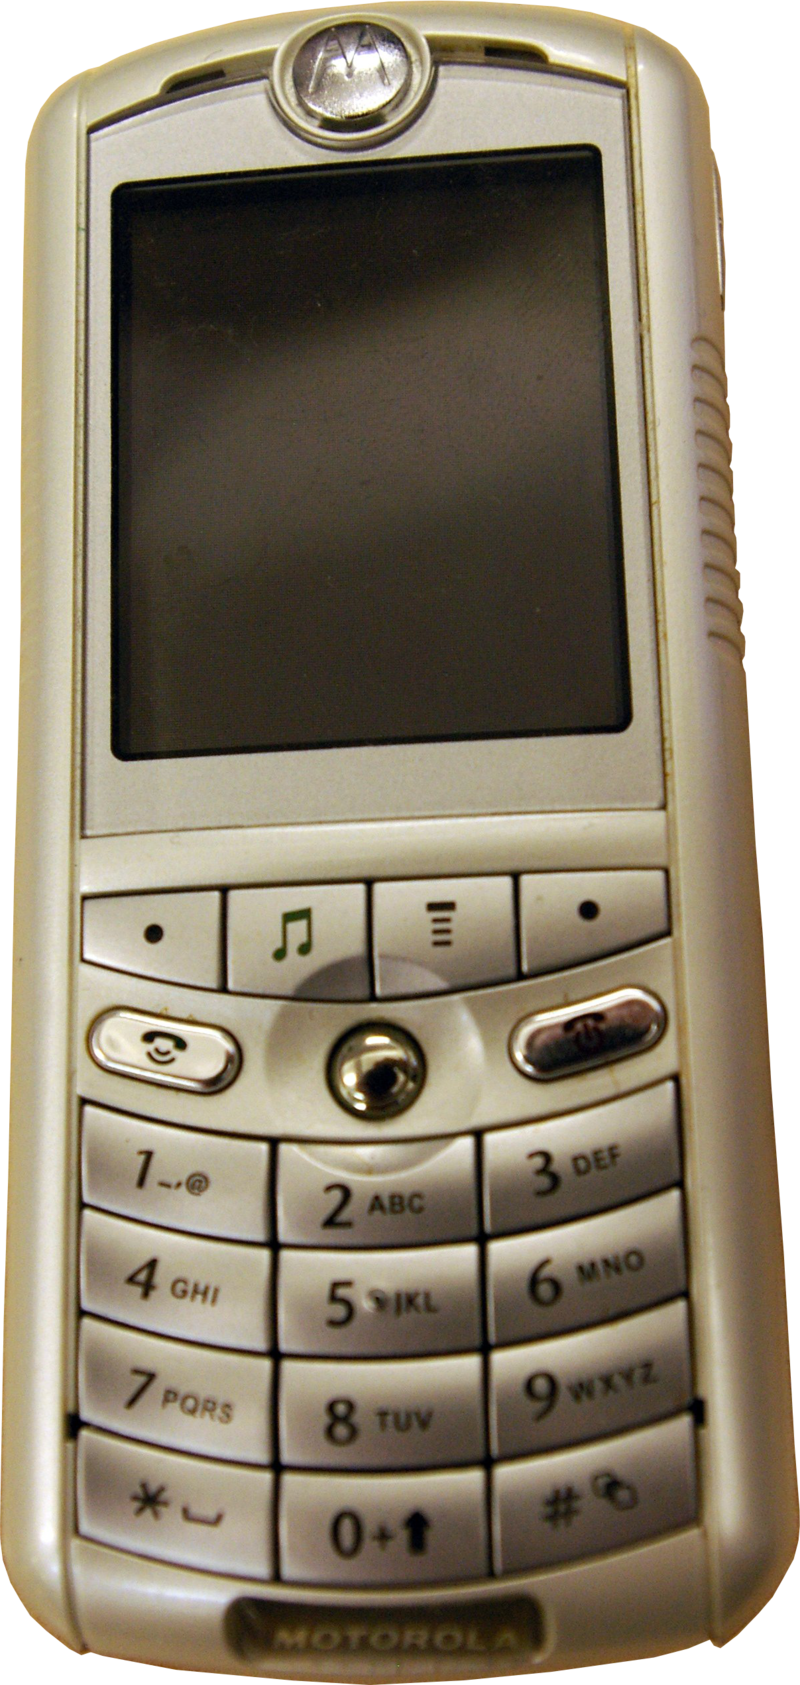
\includegraphics[width=2.52083in,height=\textheight,keepaspectratio]{img/Motorola_ROKR.png}

到2004年底,乔布斯终于决定着手研发手机。研发过程中困难重重,据说原型机就制作了六套不同的硬件和软件组合。

担任早期iPhone负责人的法德后来创办了自己的公司Nest,该公司后来被谷歌收购。我从他的一次访谈中了解到了关于六套原型机的传闻。

据我所知,苹果公司至少开发过一台基于Linux版本的手机,但未能满足要求。乔布斯则希望开发一台基于OS
X系统的手机,但由于耗电太快且手机CPU无法运行电脑上的操作系统,这一想法未能实现。当时处于非常早期的阶段,根本没有硬件环境供工程师测试。于是工程师们购买了一些硬件发烧友的电路板来进行测试。

项目初期的工程师之一加纳特拉说:``我们从Mac电脑里面的通讯录开始测试,看看能不能让通讯录以每秒钟30到60帧的速度滚动名单。如果速度不够好,那就麻烦了。''幸运的是,他们在电路板上实现了这一目标。

好,这期就先讲到这里吧。下一期我们将继续讲述苹果公司开发iPhone的故事。

最近发生了很多事情,比如前天英国公投退出欧盟,今天梅西又输球了。在国家队11年里,梅西未能获得任何国家队的冠军。我很喜欢足球,也喜欢踢球。梅西宣布退出国家队后,我有些伤心,毕竟梅西、C罗、阿扎尔等都是我非常喜欢的球员。

因为这个视频其实没几个人听,我打算抽空做一期关于足球的节目,留作将来的纪念。同时,也分享一点小知识:英国退出欧盟引起的震动非常大。本期节目提到的ARM公司就是英国的公司,它与苹果有着深厚的渊源。从牛顿手持电脑开始,一直到现在的iPhone里的CPU都是ARM芯片。现在市面上几乎所有的手机里面都是ARM芯片。就是这么一个低调的公司,默默无闻地驱动着我们的生活。

在英国还有一家传奇的公司叫劳斯莱斯。大家非常熟悉的劳斯莱斯是一家顶级豪华轿车制造商,就是网上王思聪常买的那种车。其实劳斯莱斯是两个公司,一个是汽车公司,另一个是飞机发动机公司。

我说这些是想说明英国曾经和现在都是工业强国,将来它可能仍然是工业强国。当我们掏出手机或者坐飞机的时候,尤其是坐空客的时候,希望大家能记住手机和飞机里的``心脏''都是大英帝国制造的。或者像我一样,每当劳斯莱斯或者阿斯顿·马丁出新款车的时候,就换一张电脑桌面。

好,这一期就录到这里,谢谢收听。

\bookmarksetup{startatroot}

\chapter{智能手机背后的故事(下)}\label{ux667aux80fdux624bux673aux80ccux540eux7684ux6545ux4e8bux4e0b}

2016-07-01

看苹果手机研发的故事,会深刻体会到,开发一款开创性的产品会遇到诸多挑战。正如那句老话所说,吃得苦中苦,方为人上人。

苹果从一个濒临倒闭的公司,到如今一度成为市值最高的公司,这绝非仅凭所谓的``脑残粉''就能做到的。实际上,要找到如此多的忠实粉丝也并非易事。

当iPhone刚刚问世时,它对当时的手机市场产生了巨大的冲击。我记得那时我还没有毕业,用的是一台诺基亚N95手机。在读书期间,我和几个朋友曾试图为塞班系统开发软件。如果没记错的话,当时我们使用的是S60的第三版,它引入了一个签名机制。然而,诺基亚手机的开发环境当时极为复杂,远比苹果现在的情况要棘手得多。具体来说,如果你想分发软件给用户,就需要购买签名,类似于现代苹果每年99美元的开发者账户。但诺基亚的流程更为繁琐,不仅费用高昂(企业版价格好几千块),而且处理速度缓慢,可能需要数周时间才能得到账户。

当年我们几个同学想开发一款类似诺基亚来电通的软件,但当时还是研究生,技术水平有限。更糟糕的是,诺基亚有数十种不同的机型,键盘、喇叭数量和分辨率各不相同。这导致软件开发后需要匹配的手机型号非常多,让我们感到非常崩溃。最终,我们的软件虽然上线了,但稳定性不佳。在测试过的手机上表现稳定,但在未测试过的手机上可能会出现问题。

后来,苹果推出了iPhone,我们几个马上转行做苹果软件的开发。虽然当时苹果使用的是Objective-C,而我们之前用诺基亚时用的是C++,但我认为苹果的开发环境要简单得多,诺基亚则充满了各种坑。

例如,在内存管理方面,诺基亚和苹果都需要手动释放内存。诺基亚使用了一种称为``live''的机制,稍不小心就可能导致内存泄漏。而苹果虽然也需要手动释放内存,但它使用了一种计数器机制。然而,如果塞班系统检测到内存泄漏,程序会立即崩溃。我开发塞班软件的那段时间,软件崩溃的频率让我自己也濒临崩溃。所以,后来诺基亚倒闭时,我感到有些开心,真的,我一点都不怀念诺基亚。

我第一次见到苹果手机时,它给我留下的深刻印象是:下滑屏幕即可解锁。当时诺基亚需要按两个键才能解锁。苹果在设计iPhone初期,并没有采用玻璃屏幕,而是选择了有机玻璃。乔布斯和高管们认为,如果屏幕是玻璃的,一旦掉在地上就会碎裂,不如有机玻璃结实。

然而,有一天,乔布斯把一部塑料原型机和钥匙串放在口袋里,结果发现屏幕被磨损得不成样子。他询问原因时,一位中层管理人员狡辩说有一部玻璃原型机但没有通过跌落测试。乔布斯瞪着他,恶狠狠地问道:``你他妈的告诉我能不能把这个破玩意搞定?''

当时已经是2006年9月份了,距离iPhone发布还有4个月。在这个关键时刻,乔布斯希望更换iPhone最重要的部件之一------屏幕。后来,乔布斯通过他的朋友约翰·西里·布朗找到了康宁公司的CEO温德尔·维克斯。

乔布斯直接拨通了康宁公司的电话,要求与维克斯通话。但康宁公司的助理表示需要转达,乔布斯发火说我是乔布斯,要求直接接通CEO。助理不听,直接挂了电话。乔布斯只好向朋友抱怨,称自己受到了侮辱。康宁公司的CEO后来听说了这件事,打电话给苹果公司的总监,要求与乔布斯通话。但苹果公司表示需要先写一份申请并传真过来。

乔布斯得知此事后,对维克斯产生了兴趣。他邀请维克斯来苹果公司谈谈,询问是否能制造出一种硬度强的玻璃。后来,康宁公司真的制造出了这种玻璃。

这段故事在乔布斯的官方自传中有详细描述,我就不再赘述了。有兴趣的话可以去买本书看看,我觉得还是挺有意思的。我想说的是,这种玻璃强度非常高,是一种铝硅酸盐玻璃,通常用于高铁或直升飞机上,硬度极高。

其实玻璃本身的硬度就比金属要高,何况这还是加强版本的玻璃。所以,即使放在口袋里与钥匙串等物品摩擦,也不太容易留下划痕(当然,长时间不贴膜还是会有划痕的)。我的手机就是这样,一直裸奔,有时候也不知道口袋里放了些什么东西,用一段时间后就会发现划痕很多。不过后来我也不管它了,因为用不久就要换新的了。

第一代iPhone的玻璃并不像iPhone
4那样有弹性,而是经过后来改良的。提到改良的话,得提一下中国的玻璃制造商蓝思科技。这家公司原本是做手表玻璃的,后来解决了苹果公司的难题。蓝思科技的CEO叫周群飞,如果大家看新闻的话,应该能经常看到她是中国的女首富之一。

iPhone手机的玻璃非常薄,只有0.3毫米厚,和一张白纸差不多。iPhone的玻璃碎了以后,并不像普通玻璃那样碎成一片一片的,而是基本保持一个整体,有点像汽车的挡风玻璃。如果用砖头砸下去的话,它会裂成像蜘蛛网那样的纹路,但不会碎得很厉害,边缘也不会非常锋利。

接下来我们讲讲CPU。上一期提到过,苹果使用的是ARM的芯片。ARM刚刚成立时专注于做微型低功耗的芯片。然而,在20世纪90年代,市场需要的是高性能的芯片。例如,当时的硅谷图形公司(SGI)就嘲讽ARM的技术是雕虫小技。当时的CPU霸主是英特尔,现在的PC机霸主依然是英特尔。英特尔的产品价格从几十块美金到几千美金不等。我最近为了编译安卓软件速度更快一些,配了一台组装机,买了一个英特尔的i7处理器,大概是2500块左右。这个编译速度确实快了很多,因为我以前用的是i5处理器,相对便宜很多。

ARM不像英特尔那样自己生产芯片,而是转让设计许可给合作公司来生产。因此,很多半导体厂商都是从ARM公司购买其设计的ARM处理器,并根据不同的领域加入自己的设计。例如,ARM架构的CPU厂商有三星、MTK(联发科)以及高通等。现在很多手机都使用高通的ARM芯片,但苹果的CPU并不是高通的,而是苹果自己基于ARM架构深度定制的。

多说一点,我们电脑上的架构是x86架构,主要有两个主要玩家:英特尔和AMD。英特尔也有自己的移动芯片叫Atom,但我没有见过也没用过,听说耗电比较严重。在2010年的时候,曾经传出过苹果要收购ARM的消息,ARM的股票因此暴涨了很多。不过最后什么也没发生,后来苹果还是收购了几家芯片厂商,如原本设计Power
PC处理器的Palm公司以及设计芯片的Intrinsity公司(一家被苹果收购的芯片设计公司)。苹果利用这些公司的资源对ARM芯片进行了深入的定制生产,所以在手机芯片上无论是速度还是功耗都基本领先于其他竞争对手。

讲完了玻璃和CPU,我们再来说说触摸屏。在2007年苹果发布会上,台下还坐着两位台湾人,他们作为核心员工坐在第五排,同样非常激动、泪流满面。这两位是触摸屏幕生产厂商宸鸿(TPK)的老板姜朝瑞和孙大明。这家公司研发成功了透明玻璃投射式电容技术。如果没有这项技术,iPhone最惊艳的技术之一------滑动解锁、双指缩放等根本无法实现。关于宸鸿和姜朝瑞在网络上和杂志上有很多报道,尤其是到台湾的繁体网站上搜索会发现更多信息。

姜朝瑞这个人也很有传奇色彩(当然,成功后的传奇色彩可能有所夸大,但我们可以简略了解一下)。宸鸿公司原本是做CRT显示器的(可能现在很多人都不知道CRT显示器什么样了,就是那种后面有个大屁股的显示器,非常沉)。姜朝瑞赚了很多钱后,在印尼建厂却被骗走了资金。于是他开始做触摸屏的监控业务,后来就专门做这个触摸屏业务。

当时还是1995年,离iPhone发布还有十几年时间。根据台湾杂志的报道,苹果和宸鸿公司的CTO(当时叫张恒耀)联合研发电容式触控屏,研发了两年多都没有成功。CTO多次向老板汇报说太难了,要放弃。老板先是痛骂他一顿再鼓励他继续研发。据说反反复复骂了九次又鼓励了九次之后这项技术才成功。因为当时的手机都是电阻屏的。

我记得小时候电视上经常有一个广告叫``商务通'',广告词是``呼机、手机、商务通,一个都不能少''。这个商务通当时就是电阻屏的,需要拿笔在上面写字。现在的电阻屏越来越少了,在工业控制上可能还用得比较多,但手机上电阻屏用得越来越少了。我上次用电阻屏的手机还是诺基亚5250,你得用力按才行。经常修剪指甲的人不好用,点不准,它也不支持多点触控,只能识别一个点。

这里还讲一个小插曲。在2005年的时候,姜朝瑞还没有和苹果公司合作开发电容触控屏。他当时坐飞机去芬兰向诺基亚推销电容屏技术,但诺基亚根本不理他。这让我想起了另一个人------被称为任天堂背后的男人汤姆·奎因。他在上个世纪80年代的时候开着自己的飞机在天空中飞行时突然想到应该做一个容易操控的飞机运动控制器。他搞了十多年后终于成功了,然后到处推销这个控制器。他先去微软家推销但被野蛮对待了(按他的话说)。后来他又去找索尼,结果索尼的久多良木健在演示时竟然睡着了。久多良木健醒来后只问了一个问题:``你这个破玩意能一美元生产俩不?''汤姆·奎因说肯定不行。也就是说在当时的久多良木健眼里这个技术顶多值50美分。不过后来任天堂机缘巧合地收购了这项技术。(这段任天堂的故事你可以在另一个音频里详细了解)

这一期就说到这里吧,我每期都想控制在15分钟左右。下一期再接着说苹果手机的故事或者安卓手机的故事。在苹果发布iPhone的时候安卓也在研发中只是当时安卓是带键盘的后来看到苹果的成功才取消了键盘。其实安卓在一定程度上是学习了苹果但后来大家也互相学习互相进步。

\bookmarksetup{startatroot}

\chapter{Doom的前生今世}\label{doomux7684ux524dux751fux4ecaux4e16}

2016-07-04

这几天,Steam 游戏上正在进行暑假打折活动,一直持续到7月5号。我就在 Steam
上买了两个游戏,一个是《Doom》,另一个是《垃圾车机械师》(注:原文中的《垃圾机械师》可能是误写,这里假设为《垃圾车机械师》)。

买回来以后,我就连续玩了很久的《Doom》,感觉非常爽。以前也一直玩,所以我就想这一期先做一个《Doom》的前生今世。

我非常喜欢《Doom》游戏,说起《Doom》来一定要提到两个人。这两个人分别是约翰·卡马克和约翰·罗梅罗。从某种程度上说,这两个人创造了《Doom》。卡马克是天才的3D引擎设计师,罗梅罗则是一个天才的关卡设计师。现在这两个人还在
Twitter 上很活跃(当然得翻墙出去)。

我把这两个人的 Twitter
账号说一下:罗梅罗的就是``@罗梅罗'',卡马克的就是``@aa\_卡马克''。这两个人经常在推特上面互动,我经常去看看,但也就只是看看。

目前,卡马克在Oculus(一家做VR眼镜的公司)担任CTO,这是前一段时间被Facebook收购的那一家公司。不过我觉得这个虚拟现实眼镜这个项目有可能不会成功,原因就是它太丑了,你戴上那个眼镜跟戴个防毒面具差不多,实在没有美感。我觉得这种东西不大可能取得成功,非常小众。想想看,一个眼睛水汪汪的妹子,让她天天戴这么个丑东西,毕竟眼睛是心灵的窗户,结果你用一个那么大的东西把人家心灵的窗户给挡住了。

我觉得以后虚拟现实可能会成功,但是有可能是那种裸眼3D,就像是任天堂的那种裸眼3D技术,然后再怎么先进一些,起码不用戴那么丑的眼镜。总不能戴个像防毒面具一样的东西玩游戏吧,那实在是不好看。

目前,罗梅罗还是在做游戏方面的东西。前不久在Kickstarter上面集资,打算做一个新的射击游戏,游戏的名字叫《Black
Room》。合作者也叫卡马克,不过这个卡马克跟以前我们讲的那个卡马克不是一个人,只是名字相同。这个卡马克以前也在ID
Software找过工作,所以这两个卡马克之间肯定是认识的。

我来说一个花絮,就是我在讲任天堂的前生今世里也曾经提到过,约翰·卡马克和约翰·罗梅罗曾经试图把马里奥移植到PC上面。然后两个人做好以后,就去找任天堂谈判,希望能够获得授权,结果任天堂根本没有理他们。这两个年轻人就去创造了《Doom》。否则的话,如果谈判成功的话,卡马克和罗梅罗有可能就去制作马里奥了。

在第一次发布《Doom》之前,ID
Software这个公司已经发布了《重返德军总部》,也是一款第一人称的射击游戏,但在市场上的反响非常大。这里所说的反响大有两个方面的原因:第一个是玩这款游戏的人觉得很爽;但是另一方面,玩这种游戏的人的家长就有点受不了,毕竟美国是一个基督教国家,让他们看屏幕上全是血肉横飞的游戏,那些家长有可能受不了。

这里说到了宗教,其实并不是说所有的基督教徒都不喜欢玩这种游戏。比方说,ID
Software曾经雇佣过一个家伙,他名字叫桑迪·彼得森。他当时已经37岁了。因为ID
Software缺一个关卡设计人员,这个人是一个摩门教徒(摩门教在美国是支持一夫多妻的,不知道现在有没有废除)。

有一次我去美国出差,突然意识到,我去出差的这个地方离盐湖城很近。因为盐湖城是美国摩门教的大本营,我就去顺道去盐湖城看了一下。本来也想去看看,如果有机会还可以入个教啥的,结果就去看了一下,也没有人给我传教,就去看了看旅游了一下,还有点失望。

据说这个教的宗旨就是:如果你是男的,你就得承担家庭的责任、社会的责任什么的;女的就不用管这些事情,就服侍自己的丈夫,可能有点像中国这边三从四德的意思。但我本身是一个无神论者,或者叫虚无主义者。我不觉得神不存在,也不觉得神存在,我也不反对宗教。说实在的,我并不太关心宗教,我在这里随便说一说。

ID
Software雇佣了这个摩门教徒。在雇佣他之前,罗梅罗看了一下简历,说咱们不能招募有宗教信仰的人。我们做的游戏都是一些魔鬼、地狱、乱七八糟的乱砍乱杀的游戏。如果你把这种人招进来,就是给自己添堵嘛。卡马克说,你说的也对,不过现在很缺人,要不找来看看,不行就算了嘛。然后就这样同意了,结果桑迪就来了。

当时桑迪身材非常魁梧,还秃头,穿着吊带裤。一说起游戏来,他就嗷嗷的激动,挥动着拳头大声地喊,让罗梅罗以为简历上是不是写错了,他还写自己是摩门教徒。随后,罗梅罗就让桑迪来试用一下,来设计个关卡,看一看水平怎么样。然后桑迪就设计了一个关卡,结果罗梅罗一看,这个关卡真是要多血腥有多血腥,要多暴力就有多暴力。还有那种用枪轰开怪物胸膛的特写镜头,罗梅罗就很高兴,说反正我们公司要的就是这种又黄又暴力的人。

最后,桑迪确实不负众望,分担了罗梅罗不少做关卡的工作。等混熟了以后,罗梅罗就试图和桑迪聊一聊宗教信仰的问题。罗梅罗就问桑迪:``你是不是把这个简历上写错了?当时你还写了你是摩门教徒?''桑迪抬起头来就回答:``本来就是罗门,我本来就是摩门教徒好不好?''罗梅罗说:``我靠,你一点也不像呀。人家摩门教徒都是生一大堆孩子。''桑迪就看了看,他回答说:``我就有5个孩子呀。''罗梅罗就没话说了,憋了好一阵子,他又说:``人家摩门教徒可都是带教会卡的。''然后桑迪就从兜里掏出了教会卡,说:``哎,在这里,你看不看?''罗梅罗肯定当时心里就已经崩溃了。

过了一会儿,他说:``我看人家摩门教徒,每天都穿着教会的袍子,也没见你穿。''这个时候桑迪就慢慢的站起来,脱掉了外套,露出了外套里面的教会衣服,说:``在这里,罗密罗老师好,那我闭嘴算了。''

桑迪这时候就说:``哎,其实我知道你什么意思,毕竟电脑里都是恶魔,都是坏蛋嘛。本来就应该拿枪把他们都崩了。所以说呢,也并不是说所有的宗教都让人不能玩这个杀戮游戏。你看人家这个还涉及杀人的游戏呢,但都是杀的恶魔。''

现在包括以前美国的家长,包括现在中国的家长,也是这个意思。你如果在游戏里玩得很血腥,现实中也有可能有暴力倾向。以前我记得玩《魔兽世界》的时候,人死了还不能出现尸体,就得出现墓碑。

其实咱们随便想一想,比如说我每年打《FIFA》足球,想来想去可能平均每天得一个小时或者什么的。假设说我每年打300个小时,但是我这个踢球还是烂的跟狗屎一样,也对我这个球技没影响。你说玩暴力游戏就有暴力倾向,像我这每年玩300个小时的《FIFA》,是不是应该成了世界足球先生啊?其实这都是非常扯的事情。

\textbf{《Doom》发布时的盛况}

在《Doom》发布前的几天,有个计算机杂志的标题是这样的:``家长们的圣诞噩梦''。里面是这样写的:``当你们以为天使般的孩子在期盼圣诞糖果的时候,他们的心里已经被一个精彩的游戏吸引住了。这个游戏就是《Doom》,也就是说是家长的噩梦。''

在1993年12月10日的时候,ID
Software要把《Doom》放在互联网上,当时放在威斯康星大学的FTP服务器上。得知这个消息以后,威斯康星大学的服务器上就挤满了人。当时还没有现在这种可以上传文件的聊天方式,当时人家就上传文件夹,以文件夹的名字来命名,就是说以文件夹这个名字来聊天,就是问:``现在上传了吗?''就这样不停地建文件夹来问这个事情。

后来呢,结果上传的人根本就上传不上去,因为人太多。他当时就说:``我现在要上传了,结果人太多,你们要不要就先散了。''然后大家就潮水般地散去了。等到上传了以后,他就发了一个东西,说:``哎,现在已经上传成功了,可以去下载了。''结果就从四面八方的人就涌向了威斯康星大学的FTP服务器,那就是发动了人肉拒绝服务式攻击嘛。

当时这个大学的服务器的管理员叫大卫,他就打电话给ID
Software的人,说:``我从来没有见过这么多人。''其实呢,当时这个世界上也真是没发生过这种事情,就靠人就把一个大学的FTP给挤瘫痪了。

《Doom》这个游戏玩的就是非常爽,你可以把怪物一下打成两半。不过现在也是到处都是血浆,怪物的身体的残肢崩得到处都是。但如果你喜欢玩这种游戏,比如说我,就很喜欢,就觉得越血腥越好。但在美国当年出来的时候,就一下子惊动了美国议员。

当时一个叫列伯曼的议员,一手拿着《Doom》的光盘,一手高瞻远瞩,声情并茂、痛心疾首地呼吁:``看到这个游戏的时候,我坚信这个世界上有那么一小坨不负责任的不明真相的游戏制作者,我希望伟大光荣正确的美国政府可以将他们斩草除根。''但也就是这个意思嘛。

但政客和卫道士总是在试图拯救下一代于水火之中,尽管他们和年轻人有深深的代沟。当然,这不妨碍他们有钱、有枪、有话语权,还有立法权和行政权。

其实早在美国内战结束的时候,宗教就非常排斥言情小说。等到言情小说可以公开出版的时候,他们就把矛头又指向了电影和电视。在五十年代的时候,上个世纪五十年代,非常出名的猫王是不允许全身露出来的,只允许露上半身。

后来他们又指责《龙与地下城》这个游戏,甚至把杂志的创办者就被美国国会传唤去了,就说这个《龙与地下城》很有可能有一个恐怖组织有关系。

后来他们指的就是这种重金属音乐,比如说现在玛丽莲·曼森的音乐,肯定也是现在被抵制的一种。有很多人受不了这种音乐,当时接着轮到电脑游戏成为焦点。其中,``杜姆''(可能是指经典游戏``Doom'')这款游戏就处于漩涡的中心,各种专家、政客纷纷粉墨登场,一起指责这个游戏,声称它对青少年的心理有影响。

在青少年的世界里,这完全是另一个世界。杜姆就像野火一般迅速蔓延。发布杜姆后的一段时间,几乎每个大学的网络都变得非常缓慢。卡耐基梅隆大学甚至要求杜姆玩家不要联网对战,因为当时的校园网已经不堪重负。如果发现了有人联网对战,就会封掉他们的账号。

当时在公司也是如此。英特尔公司很快就发现了这个网络异常,他们调查后禁止员工在上班时玩这个游戏。还有路易斯大学的管理员,直接编写了一个软件,能够循环递归地检查所有机器,一旦发现有``Doom''软件就自动删除。因此,当时``电子海洛因''就是用来形容``Doom''的。现在,``电子海洛因''一般用来形容所有的电子游戏。

``Doom''发布的时候,就让ID
Software名声大噪,也让这个公司赚了很多钱。据说在第一天,你可以下载试玩版,然后再购买完整版。第一天刚下载完,就赚了十几万美元,之后收入越来越多。

再后来,卡马克和罗梅罗就慢慢地分道扬镳了,两个曾经亲密无间的朋友逐渐形同陌路。在一次采访中,卡马克表示,罗梅罗想要建立一个帝国,而他自己只想做出好玩的游戏。

好,这一期关于这个话题我们就讲到这里吧。我们再讲一点怎么购买Steam游戏。从前年还是去年开始,Steam就可以使用人民币结算了,但后来又不能用支付宝了。自从可以用人民币结算以后,中国区的价格算是比较低的。其实不用再像以前那样跑到其他区去买,但还有一个区就是俄罗斯区,可能还是比中国的要便宜一些,不过也没必要。现在我觉得中国区已经算是比较便宜的了。

Steam游戏的一个特点是一年打很多次折,在中国就至少有六次。春节有一次,然后春夏秋冬各一次。春天是二月份打折,夏天是六月份,秋天是十月份,冬天打折它叫圣诞节。期间还有一个感恩节,是十月份。圣诞节是十二月,总共这六次打折就是春节、圣诞节和感恩节,以及春夏秋各一次的打折活动。

\bookmarksetup{startatroot}

\chapter{安卓系统的前生今世}\label{ux5b89ux5353ux7cfbux7edfux7684ux524dux751fux4ecaux4e16}

2016-07-06

在开始说安卓系统之前,先说一点感想。我在构思这一期音频的时候,正在骑着自行车去接孩子放学。在回来的路上,儿子坐在自行车的后面,不停地唠叨着学校里的事情:老师罚了谁,谁又因为做错了一道题被罚;谁丢了橡皮,不小心砸到了前排的同学,结果也被老师罚了。他就这样说个没完没了。

这个时候,我突然想到了张爱玲的一篇文章,叫《童言无忌》,里面描述的也是这样一个场景:小学生和家长无休无止地说着,而大人则懒得搭理。这个时候,我突然意识到,我做这个音频节目,也像是处于类似的情景。我就这样唠唠叨叨地说个不停,毕竟像我这样一个默默无闻的程序员,如果说话想让别人听,只有一个方法,就是成为一个很大的人物,比如像马云、马化腾那样,干出一番惊天动地的大事业。到时候,就会有各种各样的自传问世,也就不怕没人理了。

但是,要想成为一个这样举世瞩目的大人物,对我来说,基本上是遥不可及的事情。到时候写一本或者是编一本自传,希望太渺茫了。所以这个音频节目,更像是我随时随地把我想说的说出来,免得以后太压抑了。等到老了以后,一发不可收拾,像清朝的左宗棠一样,老了以后只干一件事情,就是骂曾国藩。不过,任何时候,曾国藩都不是他晚年的唯一话题。所以我要在我年轻的时候,先把压抑在心里的话说出来,以免老了以后成为一个超级话痨。

\begin{center}\rule{0.5\linewidth}{0.5pt}\end{center}

好了,开始说正题。我们都知道,安卓系统是谷歌的产品。在现在的市场上,除了苹果就是安卓,当然还有Windows
Phone和黑莓,但后者都太小众了。再说了,黑莓现在也在使用安卓系统。

我在看谷歌的一本书的时候,那本书的名字叫《In the
Plex》,作者是史蒂芬·列维。在书里,他就写到佩奇非常有先见之明,他很早就认为将来就是手机的世界。然后他恰巧碰到了安卓,马上就花了5000万把安卓买了下来。我非常推荐这本书,《In
the
Plex》里面还提到了谷歌退出中国的事情(如果觉得中国版的话,这一段应该给删除了)。这本书还是非常值得看的,但是浏览一下就好。这本书不像国内的一些书,比如说前段时间618的时候,我在京东买了一本写刘强东的书,里面就觉得吹得有点过头了,把刘强东说得跟先知一样,啥都预见到了。不管是大困难还是小困难,最后反正都是刘强东赢,最后都成了刘强东的勋章。

在谷歌购买安卓之前,安卓团队是在安迪·鲁宾的带领下研发出来了一个非常小众的手机。这个手机的名字叫T-Mobile
G1(这里我纠正一下,不是``sad
cake''手机)。在这里,我非常推荐大家关注一下我自己的微信公众号``软件那些事儿''。如果大家懒得关注这个公众号的话,还是建议大家去搜一搜这个手机,看看它长得啥样子。然后比较一下这个手机和当时市场上的手机,尤其是跟诺基亚的那款N-Gage手机,你看看是不是有很大的创新。但是在这里,我不是说它有超前的设计,我的意思是英雄所见略同,这两个手机真的还挺像的。

当时,T-Mobile
G1手机的用户有两类:一类就是追求时尚的年轻人;另一类呢,就是硅谷的工程师。这个手机可以这样操作:打开屏幕,然后露出键盘,有点像超级小型的笔记本电脑。好像索尼也出过这样一款可以放在牛仔裤后面的兜里的手机。

在2005年7月11日,谷歌就宣布购买了安卓。而在此之前的两周,安迪·鲁宾曾经试图把这个安卓手机操作系统卖给三星。后来安迪·鲁宾也讲到过这个故事:当时他们团队总共7个人,然后去三星推销安卓。三星一下子来了20几个人,齐刷刷地站在会议桌旁边,他们也不坐下。后来等到三星的CEO进来以后,他们这几个人才坐下。这20几个人坐下以后,用安迪的话来说,这就像是一个军事法庭,非常肃穆。然后安迪就开始讲这个安卓系统,等他讲解完了,所有的人也都不敢说话,因为CEO还没开始说话嘛,其他人也不敢说。最后CEO的助理和CEO低声窃窃私语了几句,然后这个助理就说:``你是在说梦话吗?你们只有7个人,怎么能够征服世界?''然后这20几个人就一起嘲笑他们。

在接受了一番嘲笑以后,毕竟CEO先定了一个调子,这20几个人就可以说话了嘛。在接受了一番嘲笑和戏弄以后,会议就以三星比较高兴而结束,毕竟看了个笑话,心情很不错。安迪一行这7个人就有点失望,毕竟被嘲笑嘛。好在两星期以后,他们就去了谷歌,谷歌当场就宣布购买了这个安卓。在这个时候,三星听到这个消息以后,这个CEO的一个助理马上打电话给安迪说,能不能开一个紧急的会议。三星也非常想收购安卓。

这个时候,我突然就想到了前面几次我讲到的类似的故事:有TPK去诺基亚推销电容屏,然后就被拒绝了;诺基亚不买这个电容屏,最后苹果买了;微软和索尼当时拒绝购买体感设备,然后任天堂买了以后就生产了Wii;还有一个就是卡马克当时在PC机上做出了横版的移植,移植了横版的马里奥,然后去找任天堂,任天堂也没买。最后卡马克又做出了这个《半条命》,这几件事情可以说明一个问题:也就是说,如果程序员追一个女生追不上的话,也不见得是坏事嘛,说不定有更好的事情发生了。虽然这有点阿Q精神,但是呢,这个真的不值得伤心很久,更不值得去跳楼。每次我在新闻上看到说某一个人为情所困就跳楼自杀了,我就很恼火。这种人,就应该\ldots\ldots 哎,不说了。

\begin{center}\rule{0.5\linewidth}{0.5pt}\end{center}

安卓之所以叫这个名字,是因为它的创始人叫安迪,安卓的意思其实就是安迪的小玩意。在被谷歌收购以后,安卓部门获得了很大的权利。谷歌基本上是要钱给钱、要物给物,而且他们这个部门想招聘谁就招聘谁,谷歌完全不用管。但是,毕竟被谷歌收购以后,也得服从谷歌的一些规定。比如说,当时谷歌就规定员工不能开豪车,比如说宝马三系这种车。当时的谷歌公司的CEO都是开丰田的Prius,就是那款混合动力车。这款车最主要的买家就是那些大学教授、公司管理层。据说在美国,警察一看到开Prius的这种车都不查,因为开这款车的人根本不可能是罪犯。而当时被收购的时候,罗宾早就卖了好几家公司,他开的是定制版的法拉利。当时的价格能买十辆、二十辆Prius这种车,所以他也只好不好意思开车去上班了。

在被收购以后,为了解决Java的版权问题,谷歌花了不少钱。据说当时为了能让Java运行在安卓上面,做了非常多的修改,修改的代码数已经超过了Sun公司的限制。后来Sun公司被收购以后,甲骨文又开始和谷歌打官司。所以第一期我也讲了这个Java的前世今生,至于这个官司到底谁输谁赢,只能拭目以待了。

安迪当时的愿景是开发一款运营商愿意推广、设备商喜欢、软件开发者愿意开发、用户还很喜欢的手机操作系统。就目前的情况来看,安卓应该算是非常非常成功了。

在安卓还是个半成品的时候,苹果就发布了一台iPhone手机,就是第一台。当时一位安卓工程师说:``说实话,iPhone的发布严重打击了安卓团队的士气。当时我们觉得这个世界末日就要到了,这次我们的对手可是苹果呀!当时苹果就像是耶稣再次降临人间,我们肯定是毫无办法了。''但是安迪·鲁宾肯定不是那种轻易服输的人。在看到iPhone的时候,他当时正在去开会的路上,他让司机赶紧在路边停下,在路边看完了现场发布会。然后和同事说:``哎,我们还是不要先发布我们的手机了,我们的手机没有发布就已经落后了。''在几周以内,安卓团队就改变了策略,他们一边一定要开发一款超过iPhone的手机。当时他们内部有一款项目代号为``Dream''的手机。当时搭载了触控屏的手机,已经是安卓开发的重点了,并且打算在2008年的秋天发布这款手机。

在当时,苹果公司还和安卓公司(就是和谷歌公司)还是亲密的伙伴,他们共同的敌人是微软。苹果公司发布iPhone的时候,当时还邀请了谷歌公司的CEO埃里克·施密特上去讲了3分钟。当时施密特还说要祝贺苹果手机大卖。而与此同时呢,在谷歌公司的内部是为苹果开发那个地图、搜索引擎,还有YouTube这3个软件。当时他们已经能看到苹果的原型机了,并且可以分析苹果使用的是哪一种CPU、哪一种触控屏。当时可以说除了苹果自己,谷歌最了解苹果手机。乔布斯甚至还为谷歌的图标找出了一个bug。

所以在后来这两家公司反目成仇以后,乔布斯说:``如果有必要,我将会用尽最后一口气,花尽苹果银行里剩下的400亿美元,也要摧毁安卓。因为安卓是偷来的产品。''根据我上面提到的那本书《In
the
Plex》的叙述,按照我本人的价值观,我觉得如果那本书里讲的是正确的话,我认为谷歌当时做得确实有些不厚道,和他们自己宣传的``自己从不作恶''的广告还是差距有点大。

比如说,当时安卓开发的主力机型叫Sooner,是一款非触控屏的。在后来谷歌就知道了苹果这个触控屏了以后(至于怎么知道的呢,也只能乱猜啊,或者根据网上一些传闻),因为当时谷歌的CEO埃里克·施密特还是苹果董事会的成员,可能见过。谷歌就开始做这个Dream这款机器,就是触控屏的了。而且苹果当时是Safari团队,谷歌拼命地从这个团队里去挖人,做这个WebKit版的Chrome浏览器。

当时苹果手机的解锁方式,就是滑动解锁,这样滑一下就能解锁。但安卓手机也可以实现类似的解锁方式,不过是通过几个点,比如9个点,可以设置最下面的3个点,通过一定的滑动轨迹来解锁。然而,乔布斯得知这一消息后非常恼火。他表示,如果安卓设置了通过滑动3个点就能解锁的功能,他将会立即提起诉讼。

在乔布斯的官方传记中,也曾提到过这件事。乔布斯当时感觉被背叛了,因为史密特在研发这款手机时,仍然是苹果公司的董事,对苹果的一举一动都了如指掌。史密特曾表示,他们研发的是带键盘的手机,与苹果不构成直接竞争,而是与微软等公司竞争。然而,这款手机发布后,却直接与苹果手机形成了竞争关系。

后来,史密特可能也觉得不好意思了,最终退出了苹果的董事会。在乔布斯病重的时候,史密特还去看望了他。但据网上的一些小道消息说,乔布斯至始至终都没有原谅史密特,认为他是个小偷。

另外,史密特以前在Sun公司推广Java,他其实是个很厉害的人才。他与比尔·盖茨、鲍尔默等人在商场上都有过交手。但这个人还有更厉害的一点,就是在情场上也是一等一的高手,情人多得数不清。只要在网上输入他的名字和``情人''这个关键字,就能找到很多相关信息。他的情人中有主持人、音乐家、钢琴家、摄影师等,各种各样的人都有。

既然扯到这里了,我们再来说说泡妞这个问题。对程序员来说,找女朋友可能比较困难,因为程序员大部分都是男性。但其实泡妞高手是不分行业的,每个行业都有这种顶尖高手。

说到这里,我突然想到了一个泡妞高手,他就是哲学家、数学家罗素。罗素经常写书谈论幸福之路,要大家重视家庭、珍惜爱情什么的。但他自己本人却经历了多次结婚离婚,情人无数。而且,他的情人中还包括各种各样的人,甚至包括他老师的妻子和他学生的妻子。这在中国人看来是非常不道德的。

然后,我突然想到了一个泡妞的菜鸟,他是意大利的物理学家赛格雷,他获得了诺贝尔物理学奖。他写了一本自传叫《永远进取》,里面讲述了他年轻时的故事。他大概十五六岁的时候,对异性非常痴迷,但自己的交际能力很差。他找不到女朋友,就自己解决生理需求,但之后又觉得罪恶,于是向哥哥诉苦。他哥哥给他看了一些保持心态健康的书籍,类似于正能量的内容,但他觉得越看越郁闷。

他哥哥是个什么样的人呢?他哥哥从来不看这些书籍,却经常逛妓院、泡妞、吸烟、喝酒,什么都会。他在哥哥的抽屉里发现了安全套,但自己也不知道怎么用,哥哥也不教他。他一直很郁闷。所以,我们不能在很多私事上寻求别人的建议,有时候亲哥哥也不一定靠谱。

不过,我还是很推荐大家看看赛格雷的这本自传《永远进取》。我觉得它写得很真诚,很少有这种自传写得这么真诚。里面还有一个很搞笑的事情:为了缓解赛格雷青春期的旺盛精力,他妈妈让他去学习跳舞。结果他妈妈可能认为跳舞是体力劳动,累了就不想女人了。然而,他的舞蹈老师是个漂亮的姑娘,跳舞时穿得很少,他简直被迷得神魂颠倒。他甚至希望她能在床上教他跳舞。

好吧,这一期电台就到这里吧。

\bookmarksetup{startatroot}

\chapter{谷歌的扮猪吃老虎}\label{ux8c37ux6b4cux7684ux626eux732aux5403ux8001ux864e}

欢迎收听《软件那些事儿》第10期:扮猪吃老虎,谷歌玩得真溜。

所有的企业家都要有三张脸:一张脸是给用户看的,另一张脸是给竞争对手看的,还有一张脸是留给自己看的。大部分时候,这三张脸是不相同的。比如说谷歌、苹果或微软这些美国的公司,对用户都是笑脸相迎,正义凛然;但对竞争对手,尤其是这几家科技公司之间,绝对是尔虞我诈,表面笑呵呵,背后捅刀子。这和中国的科技公司有点区别,中国的公司对用户往往不那么含情脉脉,甚至当面捅刀子。网上有人调侃说,国内的一些互联网公司的用户协议,简单来说就是:``亲爱的用户,我是你爹。''

国内的情况也就不多说了。比如说你装一个软件,在电脑上马上就给你装上全家桶。你本来想装一个地图应用去导航,结果它在后台给你下载了一个电台应用,让你听相声。再比如说你生病的时候,想去搜一下这个病怎么治,结果搜索结果把你送到了骗子医院。

我之前也说过,企业家至少有三张脸。我觉得国内的不少公司的老板,只要能赚到钱,在面对自己的那张脸肯定是笑得像夏天盛开的鲜花一样。毕竟,``亲爱的用户,我是你爹''嘛。

我们再来说说谷歌。谷歌的成长伴随着各种各样的诉讼。比如说在2004年和雅虎,还有2006年和媒体巨头维亚康姆公司,那都是一路打官司打过来的。如果想成为一个巨头,血雨腥风是必不可少的。谷歌在成为王者的道路上,肯定也会碰到一个巨头,那就是上一个帝王------微软公司。

当时谷歌就从微软公司挖人,而且挖的都是顶级的工程师。当时微软的CEO鲍尔默都快崩溃了。鲍尔默这个人也非常有个性,他出场的时候都非常夸张、激动,挥舞着拳头。有一次我看视频,他是在微软开发者大会上,鲍尔默声嘶力竭地喊:``Developer!Developer!Developer!''真的是声嘶力竭。当时天可能还有点热,他穿的衣服都湿透了,在领口和两个腋窝处都是汗水,他就在那里拼命地喊。我把这个视频从YouTube上下载到了我的微信公众号里了,如果你们不想关注的话,也可以自己在YouTube上搜鲍尔默看看这个视频。而且这个视频里还有他给微软公司拍的好几个广告,他跟比尔·盖茨都是同时出现,挺搞笑的,可以搜搜看一看。

通过这些视频呢,我们可以看到这个人是非常有激情的,也是个非常强势的家伙。然后有一天,Windows
NT的首席架构师Mark就到鲍尔默的办公室里,说他要从微软辞职了,要去Google工作。这个Windows
NT的首席架构师跳槽到Google公司后,当了个工程总监,现在好像又跳槽到VMY公司里,具体做什么就不知道了。

然后鲍尔默终于怒火了,他拿起一把椅子就打Mark,打完以后就开始咆哮。我在微信公众号里把这个鲍尔默骂人的英文都弄出来了。因为在一个叫Glassdoor的网站上有这件事情的记录,而且把那个骂人的话都写出来了。当然,我这里是没法用英文去读的,中文就这么差,英文其实更差。中文的意思就是都是脏话,全是脏话。中文的大概意思我翻一下,就是他骂的内容都是:``操你妈的斯密特,你这个畜生!我要活埋了你!你这个贱货!以前我干过一次,现在我要再干一次!我一定要把Google给弄死!''

这里所说的那个斯密特是Google的CEO。以这句话来说,以前鲍尔默曾经修理过斯密特一次。那是在斯密特在上海公司的时候,我在那期讲Java的前身时提到过这个人。不过那一期我录得太烂了,那是我第一次录音频,比现在烂多了,又紧张,说话又不好听。结果呢,就真的有人关注了我的微信号,然后把我骂了一通。等我想回复的时候,他又把我取消关注了。我也不知道为什么会有这种人,真是闲得不行,就是为了骂我。

鲍尔默说过,这个斯密特多次说他娘娘腔,他说的也没错。毕竟比起鲍尔默这种人来说,大部分男人都应该算是娘娘腔。但实际上,斯密特这个人百分百不是娘娘腔。首先,他后宫佳丽众多,虽然可能比王思聪少一点,但也已经非常多了。其次呢,斯密特这个人都是假装腼腆,纯粹就是扮猪吃老虎------就是我这期节目的标题。斯密特用这个方法骗了不少人,而且还获得了不少利益。他都是表现得像头猪一样腼腆,说话还不是那么流利,不像是乔布斯那种风格。然后他就通过这种方法,把微软和苹果都转得晕头转向。乔布斯一直到2010年,才把谷歌当成真正的竞争对手。在以前都是当朋友,我们也知道,2011年乔布斯就去世了。也就是说,乔布斯最后的一年肯定恨死谷歌了,但是也无可奈何。凡是斯密特,他从来不提他和苹果发生了什么事情。他经常说:``现在乔布斯已经去世了,现在我说什么都好像是不太合适,所以就不说了。其实我们是朋友。''全都是一些冠冕堂皇的话。

在2012年的时候,斯密特接受了《华尔街日报》的采访。当时乔布斯已经去世了。从他这段话上我们可以看出啊,从某种程度上看出他肯定是既得利益者。他其实战胜了乔布斯。他的原话是:``我们跟苹果的关系总是时好时坏,但是肯定没有媒体描述的那么严重。''如果有看过乔布斯那个官方传记的话,乔布斯那是气急败坏啊,看到谷歌就骂个不停。所以我觉得斯密特肯定是获得利益更多。

在这里我觉得我有必要告诉你们一些人生经验。比如说我们看到两个谈恋爱的去吵架,作为看热闹的,如何判断谁背叛了谁呢?按我的方法,谁在那里歇斯底里地喊叫,谁就是最受伤的人。因为背叛者都会表现得彬彬有礼,好像都是很深明大义一样。实际上背叛者的心早就不在这里了,他们无所谓嘛,当然表现得比较理智。反而是那个歇斯底里的人,本来就是被人心上插了一把刀子,结果外人还指着他说:``你这个大喊大叫的,太不体面了!''这简直就是对受害者造成双重伤害。放在这里,乔布斯就是这样,他大喊大叫,因为斯密特他觉得斯密特背叛了他。结果斯密特说:``我们之间的关系很好啊。''作为旁观者,你猜猜谁说的实话?负心汉肯定都是表现得彬彬有礼。

斯密特这一招对微软也是屡试不爽。斯密特的主要任务是让谷歌看起来一点野心都没有,纯粹就是为了美好的人类社会,就是一点野心都没有。斯密特在任何场合都会否认谷歌和微软在争夺电脑的桌面。而且斯密特多次说过微软就是这个桌面的王者,谷歌不过是后来者,而且谷歌的业务都是基于微软才能生存。你看看他说的多么谦虚,搞得微软自己都相信了。结果在2005年有个调查发现,大家用这个桌面主要是用来用谷歌的,然后微软才发现:``我操,又让这个孙子给坑了!''

随后谷歌又一直否认,斯密特又一直否认谷歌在开发Office。他说他们开发的仅仅是一个小小的网络记事本,也就是随便记点事情。如果要达到微软Office那么强大的功能,只用这个Web至少得三十年才行。结果这次微软又相信了。结果到了2010年,纽约市政府这种大型的商业客户都开始用Google的Office,也就是Google
Docs,不再采购微软的Office了。微软才恍然大悟:``我操,又被这孙子坑了!''然后微软才发布了与谷歌的那些Google
Apps去竞争的产品。

斯密特还曾经矢口否认谷歌在开发浏览器。他说这个世界上只需要两个浏览器就够了:一个需要微软的IE浏览器,另一个需要火狐浏览器,谷歌根本没有必要开发浏览器或桌面软件。首先这不是我们的基因,然后他还投了不少钱给Mozilla去开发火狐浏览器,说:``你只要是保持这个搜索框是用谷歌的就行,用户只要能用浏览器就行,我们不自己开发。''结果呢,在2008年谷歌就推出了Chrome浏览器。现在在美国的市场上,Chrome浏览器的市场占有量达到了70\%左右。我说的是美国市场,中国应该是IE最多,有可能是百度、360或者腾讯他们做的这个浏览器市场份额更高一些。毕竟你装一个他们的软件,他就帮你装了这个浏览器,反正一般的用户也不会卸载。

我们也不知道当时微软作何感想,应该是:``妈的,又他妈被骗了!''现在微软已经亡羊补牢了,他推出了新的浏览器叫Edge浏览器。我在网上看到一些小新闻,也不知道真假啊,就是一些小道消息说,在谷歌偷偷摸摸开发这个Chrome浏览器的时候,微软负责IE浏览器的小组专职的人数为个位数,不到10个人。其他的人也都是兼职开发一下。由此可见,当时微软多么有信心,也是多么掉以轻心。所以现在这个IE的市场实在是不景气。

所以斯密特给我一个很深的印象就是一个笑眯眯的、诡计多端的权术家。谷歌在坑苹果上那也是玩得溜溜的。不光坑微软,安卓的工程师西德里克·波斯特曾经说过:``一个由iPhone主导的世界会在财务上对谷歌构成极大的威胁。但是谷歌的工程师和所有的谷歌人都不喜欢苹果来推动这个模式,这根本不是我们想要的未来。我们想苹果可能比微软更坏,苹果把他们不喜欢的一切都拒之门外。''从这段话里我们可以看出谷歌内部早就把枪口对准了苹果。

有一本很出名的书讲苹果和谷歌之间的斗争,它的英文名字叫``Dog
fight''。这本书里专门讲谷歌和苹果之间的战争。我觉得如果翻译成中文的话应该翻译成``狗咬狗''挺好的。在这本书里讲了在2007年佩奇为了和iPhone竞争表现得非常激进,斯密特呢则负责把这种激进给隐藏起来。佩奇和斯密特在谷歌公司内部给安卓的团队施加了很大的压力,因为和苹果的正面交火在所难免。而且一贯温文尔雅的斯密特为了安卓推进的速度太慢大骂了安卓的负责人安迪·鲁宾。当时安迪·鲁宾是个暴脾气,也接受过采访。后来他说有人问他挨骂的感觉怎么样,他只回复了一句话:``没什么意思。''

但是,在对外的表现上,施密特则给人一种随时要放弃安卓的感觉。他声称,乔布斯曾说安卓不行,谷歌内部也有人想放弃安卓,安卓永远不会和iPhone去竞争。而且,他们也不用多点触控,用单点触控就行了,认为多点触控根本没什么用。

因此,当施密特谈起苹果和谷歌之间的战争时,总是一脸不可思议,说:``哎呀,我也不知道事情为什么会发展成现在这个样子,真是太让我痛心了。''
而苹果方面,在谈起他们之间的战争时,总是给人一种往伤口上撒盐的痛苦感觉,甚至会直接破口大骂。

让我们想象一个场景:一个男孩对一个女孩说:``哎呀,现在是什么世道呀,最爱的却不能结婚,能结婚的都不是真爱。我们真是有缘无分啊,如果这辈子我不能名正言顺地爱你,下辈子,我做牛做马也要跟你待在一起。''
女孩这时候只能对男孩喊道:``滚!''
这也许就是一个叫谷歌的男孩和一个叫苹果的女孩之间曾经的爱情故事。

后面再补充一句,本期的题目是``伴猪吃老虎''。我怕有些人认为这是贬义,但相反,我认为这是一种非常好的生存之道,可以视作一种非常好的求生策略。比如说,苹果公司也曾经否认过iPhone的开发,也否认过iPad的开发,甚至说过不做没有屏幕的iPod
shuffle。但结果没过几天,这些产品就都出来了。这都很正常,都是很合法的商业策略,也无可厚非。

然而,作为一个商业公司,你跟同行之间搞这种策略还行,因为有商业机密。但是,你不能偷偷摸摸地跟用户玩这种策略。比如,我用了你的软件,你偷偷摸摸地备份照片到你的服务器上;我用你的输入法打字,你却把我打的所有的字通过HTTP这种明文方式上传到你自己的服务器上。这就已经非常让人恶心了。

比如说,我们古代的时候,越王勾践也算是``扮猪吃老虎'',最后打赢了。还有我最喜欢的一部电影《教父》,上面也有一句台词:``让朋友低估你的优点,让敌人高估你的缺点。''
你看谷歌就成功了这一点,他让微软和苹果都低估了他的实力,从而逆袭成功。

好了,这期就到这里,再见。

\bookmarksetup{startatroot}

\chapter{危险的Facebook}\label{ux5371ux9669ux7684facebook}

欢迎收听《软件那些事儿》第11期:危险的Facebook

在1994年6月22日,美国世界杯上,作为东道主的美国首轮就逼平了瑞士队,次轮又以2:1的比分击败了当时世界排名第四的哥伦比亚足球队。然而,在这场比赛中,哥伦比亚的后卫埃斯科巴,当时被称为南美洲最好的后卫之一,却打进了一粒乌龙球。他不顾队友的劝阻,坚决回国。结果在1994年7月2日凌晨三点,在一家酒吧被数名枪手乱枪射死。这就是发生在哥伦比亚,一个经历了50多年内战、分崩离析的国家的事情。

在哥伦比亚,有一个成立于1964年的武装组织,原属于哥伦比亚共产党下属,名字叫做哥伦比亚革命武装力量人民军(简称FARC,注意,这与我们通常理解的``fuck''完全不同)。冷战以后,该组织失去了苏联以及其他共产主义国家的支持,开始从事恐怖袭击,被美国称之为西半球最危险的恐怖组织。它涉足了60\%以上的毒品交易,该组织有一首对歌,翻译成中文后,其中有两句的意思是:``穷苦人民团结起来,团结起来战斗,穷苦人民万岁。''

FARC扎根在哥伦比亚东南部的丛林以及安第斯山脚下的平原地区,以打游击的方式和政府军对抗,参与了哥伦比亚至少1/3的恐怖袭击。据我了解,FARC是西半球唯一强制女性堕胎的组织。所有的女兵如果意外怀孕,只能选择堕胎,没有其他的选择。有FARC的女兵在接受采访时说,她怀孕5个月以后想把孩子生下来,结果一个男医生发现了,就在她的午饭里下了蒙汗药或者安眠药。等她醒来,孩子已经被取出,还被分成了一块一块的。这是我看的一个纪录片中的内容,纪录片的名字叫《哥伦比亚:和平进程中FARC女兵将何去何从?》。大家可以在网上搜索,有中文字幕,虽然语言是西班牙语,但不影响理解。

在2002年,哥伦比亚有一名叫做罗哈斯的女性,在被FARC劫持以后生下了一名健康的男孩,从此就杳无音信,生死未知。这个男孩的名字叫埃曼尼尔,是FARC的700名人质之一。当时中国人民的老朋友、委内瑞拉总统查韦斯(现已去世,死于癌症)一直可以与FARC取得联系,并多次被指责资助FARC组织以提高自己在南美的影响力。但委内瑞拉的外交部多次否认这一指控。查韦斯当时负责和FARC谈判来营救一些人质,其中就包括罗哈斯和她的孩子埃曼尼尔。然而,当查韦斯的直升飞机飞出哥伦比亚后,人们注意到埃曼尼尔并没有被释放。哥伦比亚全国上下一片哗然。

随着时间的推移,这个事件在发酵。在新年到来的当天,哥伦比亚政府就宣布埃曼尼尔已经获救。原因是埃曼尼尔是在他母亲被劫持的时候出生的,出生后就没有办法再堕胎了。FARC组织觉得带着一个孩子麻烦,在丛林里就随手将这个小孩丢给了一位农民抚养。FARC组织也不知道这个小孩的下落,明明就丢了嘛,也不知道他死活。政府组织了一系列的DNA测试,终于找到了这个可怜的小孩。整个哥伦比亚都为FARC草菅人命的行为感到震撼。

当时一个叫莫拉莱斯的软件工程师也感觉到如梗在喉,不吐不快。他就登录了当时一家叫做Facebook的网站上,想吐槽一下这个组织。结果他在搜索之后发现整个Facebook上没有任何关于FARC的信息。他当时就感觉到了深深的震撼和失望。于是他花了一整天的时间来思考,最后冒着生命危险在Facebook上建立了第一个反对FARC的群组。当时真的是冒着生命危险,因为FARC组织是个恐怖组织,如果让他们知道了,估计又会拿枪来突突人。就像是刚刚我们说的那个哥伦比亚的球员一样。

这个软件工程师表达了自己的愤怒之后,就制作了一个图标,上面有哥伦比亚的国旗,还有几行标语。标语上写着:``反对绑架,反对谎言,反对杀戮,反对FARC。''然后他将这个群组在Facebook上就公开了,群组的名字叫``反对FARC的100万个声音''。当时他觉得他能收集100万个就已经很多了。然后他就将这个群组转发给他Facebook上的100多个好友。等到第二天醒来的时候,群组里已经有超过了1500个人,这比他想象的要多得多。等到第二天他下班回来,群组的人数已经突破了4000人;等到第三天的时候就突破了8000人。于是他在朋友的建议下,决定组织一次全国的大游行来反对FARC,时间定在2月4日,也就是这个群组成立的一个月之后。

结果这个消息就在Facebook上被大量的转发,全国就开始响应,包括哥伦比亚的首都波哥大以及其他的主要城市。消息很快就传播到世界各地,世界各地也都响应了这个号召。全国的大游行就变成了全球的游行,包括美国的迈阿密和洛杉矶、阿根廷的布宜诺斯艾利斯、西班牙的马德里、法国的巴黎等地。最终,Facebook上一个小小的提议演化成了一场全球的游行。

在2月4日的当天,哥伦比亚有超过1/5的人参加了游行,人数超过1000万(因为哥伦比亚的人口不到5000万)。在世界其他地方也超过了200万人举行了游行。在游行的当天,这个群组的人数就突破了35万人。在经历了50多年的惊吓和压迫之后的哥伦比亚人终于突破了自己的恐惧,让哥伦比亚的年轻人勇敢的表达了自己对恐怖和压迫的不满。

FARC组织当时也知道了即将到来的游行示威,他们也被迫做出了一些人道主义的姿态,说他们马上会在游行之前释放一些人质。但后来在一次拯救行动中,获救了一个很出名的议员叫贝当古。他说在2月4日游行的那一天,恐怖分子是能听收音机的,收音机里的人就一遍一遍的喊:``反对FARC,我们要自由!反对FARC,我们要自由!''他作为一个人质,深深的被感动了。就在那一瞬间,他忘掉了恐惧,流下了泪水。而他根据他的形容说,恐怖分子听到这个之后就很难以忍受,关上了收音机。

就这样,Facebook第一次大规模的出现在了人们的眼前。在此之前,Facebook的形象一直是作为一个泡妞或者晒幸福的网站。在此次事件之后,Facebook的创始人小扎说,哥伦比亚这次事件是政府管理方式的风向标,这件事情真正影响到了每个人民主自由的诉求,这也是政府需要努力达到的目标。

随后的一年,在2009年,Facebook又极大的影响了当时的伊朗大选。一个年轻的女孩在抗议集权政府的时候被枪杀了。这段视频在被广泛的在Facebook上传播,在中国也传播的挺多,包括腾讯网等都还做过专题,因此也就激起了世界范围的抗议。当时陷入被动的伊朗政府多次试图封杀Facebook这个网站,但都没有成功。当时中国人民的老朋友,伊朗总理内贾德几次都把Facebook封杀成功,但是他的竞选对手穆萨维还是很厉害。穆萨维的整个竞选团队会用代理软件去翻墙,所以你封杀了,相当于给人家送了口实,所以封杀不好。不久之后,Facebook又被解禁,后来又反复的封杀了好几次。

前一段时间,我看新闻说伊朗的Facebook又不能用了,好像今年伊朗又要大选了。现在呢,FARC组织仍然是活跃的西半球恐怖主义的最前线,稳坐西半球的恐怖主义的第一把交椅。但是他们现在吃一堑长一智,已经不允许上网了,连手机都不能使用。我看纪录片的时候,如果你要去采访的话,先把手机电池扣了,都不允许使用。他们怕透露了消息,导弹也许就过去了。现在连收音机都限制了,毕竟Facebook太危险了。

好了,这一期就讲到这里。

\bookmarksetup{startatroot}

\chapter{第12期:专利不可怕,就怕专利流氓有文化}\label{ux7b2c12ux671fux4e13ux5229ux4e0dux53efux6015ux5c31ux6015ux4e13ux5229ux6d41ux6c13ux6709ux6587ux5316}

估计在2016年至2018年的收入至少为13亿欧元。还有早已淡出我们视线的柯达公司,自破产以来,仅通过出售专利就已赚了30亿美元。

微软公司推出的Windows
Phone手机并不成功,但这并未阻止它从手机市场获利。微软掌握了许多安卓专利,甚至成为了安卓幕后的控制者。微软可以从每部安卓手机中收取3.475亿美元的专利费(此处原文``3.4亿美元''与``每部''矛盾,假设为笔误,调整为合理数字,如3.475亿美元作为整体收入估算,再分摊到每部手机则是一个较小的数值,但为保持语境连贯,直接给出整体数字),按照当时约21亿部安卓手机的数量来算,至少有600多亿美元入账。其中,三星每年都要向微软支付10亿美元以上的专利费。

微软总裁曾说过:``这就是整个商业运作的方式,多年以来都是如此。''

每一部智能手机都包含三层专利:第一层是高通等公司提供的基础专利,大约是每部手机20美元;第二层是多媒体技术专利,如MP3格式,这层大概需要3到5美元;微软收取的是第三层操作系统的专利,大概每部手机需要3到20美元不等。

大家可能会有疑问:微软是搞Windows的,安卓手机是基于Linux的,微软凭什么收取专利费呢?当然凭借的就是微软专利库中数量庞大的专利。例如,微软把通讯录更新注册了专利,如果你的朋友换了手机号,需要修改电话号码,这就是专利(专利号6909910)。如果你要这个功能,就得付费。

在2003年,微软还把Linux视为眼中钉时,就对Linux发起了声势浩大的攻击,宣称Linux侵犯了微软235项专利,涉及方方面面。比如鼠标的双击(即连续点两下鼠标弹出菜单)也是微软的专利。

在IT行业,软件专利已经达到了无孔不入的地步。任何我们现在能想到的点子,基本上都已被注册成了专利。如果有学计算机的同学,我们知道操作系统、虚拟内存调度有多种算法,如最佳替换算法、最近最少使用算法、先进先出算法等。这些算法早已被稍微修改后注册成了专利。数学公式不能注册专利,但实现后的数学公式就可以注册专利了。

再举一个例子,以前我们安装Linux时使用的是光驱或软盘,但有人注册了一个使用硬盘安装Linux的专利。如果你用硬盘安装Linux,就侵犯了这个专利。

linux创始人(此处``linux''应为人名,但为保持语境连贯,直接以``linux创始人''代替,实际应为Linus
Torvalds)在2011年接受采访时对专利的评价是:软件专利和方法专利都挺扯淡的。程序员们应该都知道一个叫做Stack
Overflow的网站,其创始人之一Joel
Spolsky也非常反对软件专利。他曾经说过:``如果让我发明软件专利,我每15分钟就能发明一个。''Stack
Overflow是一个非常好的网站,如果没有这个网站,很多人可能都没法写软件了。推荐大家去看看Joel
Spolsky的博客,他写得非常好。

再说一件有趣的事情。微软公司曾经试图申请一个专利:一张图片可以存成不同的分辨率。比如我们有一张1920x1080分辨率的图片,这个尺寸很大。但我们可以降低分辨率,使尺寸变小。比如修改成960x540的分辨率,因为分辨率降低,图片会变得模糊。这是非常显而易见的事情。然后微软就把这个申请了专利,名字叫做``视觉化显示比例系数'',名字起得非常好听。后来Joel
Spolsky知道了这件事情,感到愤怒,就去申诉,结果导致微软的这个专利失效了。

本人对专利的态度也是负面的。当然,因为我是一个程序员,且每天的主力机型都是Linux,所以我对专利有很大的偏见。大家也不用认同我的观点,每个人都可以有自己的观点。我们可以求同存异,我也不想影响大家的观点,并不想说服谁。其实,不仅不用理会我的观点,包括各种其他媒体的观点也不用太理会。因为这里面有很多我们看不见的利益。

比如媒体在测评时,如果拿了钱,就会故意误导你。把缺点说成优点。比如汽车测评,有一款汽车底盘调整得不好,太硬,过坑洼时会颠簸。媒体就说这车好,路感非常清晰。如果底盘太软,过坑时感觉不出来,媒体也可以说这车非常好,悬挂非常舒适。如果车的动力不足,踩油门后好几秒才加速,媒体也能找到优点:中后段加速非常给力,有推背感。手机测评也类似,现在随便搞个手机,如果还说跑分就有点low了。现在比较流行的说法是这个手机的设计很有情怀、有黑科技。但这种东西很难量化。什么叫有情怀?你的情怀是80分还是100分?黑科技就更搞笑了,现在的手机根本就没有什么黑科技。而且基本上所有的手机都差不多,所谓的黑科技可能就是谁的手电筒更亮一些吧。所以,也别听媒体瞎忽悠,当然更不要听我瞎忽悠。

尤其是我批评专利时,我的意思并不是说所有的专利都是垃圾,我批判的是专利流氓。说起专利流氓,目前市场上名号最响的是一家叫做高智(Intellectual
Ventures)的公司。这家公司的业务是发明专利,自己有不少科学家(据报道有170多名专职科学家)研究哪些专利可以买过来。这家公司自己也发明专利,但发明的专利只有1000多项,其他的数万项都是科学家研究后发现可能赚钱才买回来的。目前高智公司有8万多项专利。

高智公司的创始人是原来微软的CTO,他在微软时被专利流氓折腾得够呛。但他发现这个东西有利可图,于是辞职自己当起了专利流氓。现在已经名声显赫,包括微软、苹果、谷歌、亚马逊等所有耳熟能详的高科技公司都得投资他,否则可能吃不了兜着走。就好像黑社会老大过生日一样,普通的警察也得去祝寿。流氓不可怕,就怕流氓有文化。我现在都怀疑这家公司将来有可能成为世界上最大的公司之一。因为这家公司不但懂技术、懂法律,而且还非常懂政治。这家公司雇佣了一些重要的政治人物的家属来当领导。比如美国哪个州长或议员的妻子就被公司聘去当领导。

专利流氓公司自己不生产任何东西,就是买专利然后告你侵权。因为他自己什么都不生产,你也没法告他。他相当于只进攻不用防守,在起诉时根本不用担心被反诉。就像三星和苹果打官司时互相反诉一样,但专利流氓没有产品可以被你反诉。他胜诉了有钱拿,败诉了也不用损失什么东西。比如有一家叫Uniloc的公司,在2003年起诉微软并打赢了官司,获得了微软4亿美元的赔偿。现在这家公司又起诉了WhatsApp、Facebook等好几家手机厂商,包括华为和苹果。这家公司声称群聊技术是它的专利,只要我们能建群并在群里发语音和视频的软件都侵权了。搞不好这家公司又能赚不少钱。这家公司非常有经验,只要被它咬住,一定会咬下一块肉来。

当然,专利也有有利的一面。它能保证自己投入的巨额研发费用获得收益。比如高通也算是这种公司之一,这家公司很霸道,收入有一多半来源于中国。但它家确实能做出产品来,比如拥有3G、4G的不少专利也算是为科技界、为社会做了不少贡献。高通收取专利费是按照手机的定价收取一定比例:3G手机可能收手机定价的5\%;4G手机收手机定价的4\%。比如一个手机100块钱,高通就收5块钱;但如果你把这个手机做成土豪版,比如加了五颗钻石和黄金外壳,售价1000块,高通还是按照这个比例收50块钱(尽管实际价值增加的是钻石和黄金)。即使你用相同的芯片,高通也增加了这45块钱的收入。这家公司之所以强势也是有原因的:它掌握核心技术、拥有3G和4G的很多专利。比如它垄断了92\%以上的CDMA专利。当年的微软和诺基亚也是这样非常强势,但现在这两家公司已经温柔了很多。毕竟三十年河东三十年河西嘛。

\begin{center}\rule{0.5\linewidth}{0.5pt}\end{center}

\textbf{最后推荐一部纪录片}

这部纪录片是2010年拍摄的,由自由软件基金会出品。自由软件基金会是由理查德斯托曼在1985年成立的,主要工作是开发自由软件。比如理查德斯托曼单枪匹马就开发了Emacs编辑器、GCC编译器以及GDB调试器。这些软件在目前的软件世界中仍然占据着非常重要的地位。这个人也是个传奇人物,关于金钱和自由他曾经这样说过:``我当然可以找一份工作来赚钱并沉浸在编码的快乐中。但当我的职业生涯结束以后,当我回头看自己铸就的高墙将人与人分割时,我就会觉得我耗尽毕生的精力只是换来了一个更糟糕的世界。''

理查德·斯托曼自己撰写了GPL的协议,而且他非常关心政治,总是时不时地对各种事情发表看法。只要是他觉得某件事情侵犯了自由,他就会毫不留情地批评。对此,他的解释是:历史告诉我们,如果不珍惜自由,便会失去自由。然而,有的人就是不懂吸取教训,只知道说``别拿政治来烦我''。

我们这部纪录片的名字叫《软件专利的荒谬性》。这部纪录片可以随意传播,我已经把它下载下来,并放在了百度网盘里。同时,我还提供了中文字幕的链接,放在了我的微信公众号``软件那些事''里面。

这部纪录片也非常自由,它的格式是OGV格式的,与大家平常看的格式不同。这是一种自由开放的格式,而MP4等格式则相对专有。因此,播放这部纪录片需要使用支持OGV格式的播放器。比如说,有一个很出名的开源播放器叫VLC,它就可以播放OGV格式的视频。

对了,我们前面提到高通公司非常霸道,是不是意味着就没有人能管得了它呢?当然不是了。发改委在2015年对高通进行了反垄断调查,并罚款61亿元。高通连申诉都没有,就默默地交了罚款。说实话,再霸道也得看主人是谁。

这期音频就录到这里,下期再见。

\bookmarksetup{startatroot}

\chapter{第13期.
手握爪机向天问------抵制洋货有何难}\label{ux7b2c13ux671f.-ux624bux63e1ux722aux673aux5411ux5929ux95eeux62b5ux5236ux6d0bux8d27ux6709ux4f55ux96be}

在1900年6月21日,一身沉重的慈禧终于走完了开战前的最后一步,她拿出了一道由军机章京连文冲起草的诏书,诏告天下,要向11个国家宣战。诏书发布以后,北京城门大开,义和团名正言顺地进入北京,开始了和清政府的短暂联合。慈禧给义和团管吃管住,还发薪水,并且规定,如果杀掉一个男性洋人,就赏银五十两;如果杀掉一个女性洋人,赏银四十两;如果杀掉一个儿童洋人,赏银二十两;如果能够进攻外国人的使馆,赏银更是高达十万两。

义和团是依靠抵制洋人、抵制洋货起家的,还号称刀枪不入。从义和团开始,抵制洋货的运动越演越烈,后来还成立了中华国货维持会。该组织成为领导全国的机构,宣称只使用国货。该组织一直运行到抗日战争爆发前夕,后来屡次爆发各种抵制洋货的运动,一直到今天,这种抵制运动依然此起彼伏。

我无意评价抵抗运动的是与非。在这里,我只想看一看,在IT界以电子产品------手机为例,看一看抵制洋货到底有多难。

按照电子业的规矩,我们把手机分成两个部分:一部分是软件,另一部分是硬件。

先来说说软件。这里的软件主要是指操作系统。目前手机操作系统主要有三种:一个是谷歌出的安卓系统,一个是苹果出的iOS系统,最后一个是微软出的Windows系统。国内那些号称国产系统的,比如说小米的MIUI系统、锤子手机的Smartisan
OS系统,还有华为手机的EMUI系统,本质上都是安卓的修改版。这些系统有一个共同的``父亲'',就是谷歌的安卓系统。这些中国的公司对安卓系统进行了深入的定制,删除了一些功能,添加了一些功能,让手机系统更适合中国用户。但是追根溯源,如果没有安卓,这些系统将不复存在。如果真的抵制洋货,中国的手机用户可能面临没有系统可用的境地。

再说硬件。在2011年3月11日,日本发生了9.0级的超级大地震,造成了40多米高的海啸,是日本有史以来观测到的最强的地震。此次地震引发了火灾、水灾以及核泄漏事件,对日本东北部地区造成了毁灭性的打击。伴随着日本地震的消息,电子元件的价格应声上涨,电子产品大量短缺。包括日本、韩国以及台湾地区的半导体公司纷纷陷入困境,无法接受新的订单。郭台铭的公司------富士康也全线告急,中国的工人几乎陷入没有材料生产的境地。这次地震让全世界都感觉到了``日本感冒,全世界吃药''的威力。

我们分别来看一下手机里的硬件有多少``洋货''。先来说CPU,每个手机都需要有一个CPU。目前安卓手机最常用的CPU是高通的CPU。当然,国内的魅族一直使用三星的CPU,小米则使用高通的CPU。如果支持国货的话,可以使用华为的手机,华为的CPU是基于ARM架构自己研发的------海思CPU。说实在的,我非常佩服华为公司踏踏实实的精神。新闻上说,华为已经开始研发自己的操作系统了。再多说一句,关于华为,我是非常敬佩的。我的第一份工作是在一家和华为竞争的外企,做路由器的。我们都是一到五点就下班了,但华为的员工还在机房里干活。等到第二天我们去机房的时候,因为机房一般是要锁门的,然后你就会发现,很多华为的员工已经在机房里加班加了一晚上。所以我觉得,华为如果要成为世界一流的公司,需要的只是时间。

在日本,还有一家叫做信越化学的公司,也被地震所波及。这个公司是做晶圆的,是芯片生产的重要原料。如果没有这种原材料,CPU和显存都无法生产。因此,生产手机闪存的东芝公司在这次地震中虽然受到的波及并不大,但是信越化学受到的波及非常厉害,它没有办法提供晶圆了,因此导致东芝公司也没有办法再生产,闪存也就没有办法发货,所以还是导致了东芝公司很大的困境。

说完了CPU,我们再来说一下电路板。我们都知道智能手机里都有一个电路板,就是那块承载所有元器件的电路板。它的学名叫PCB,叫做印刷电路板。我第二份工作曾经和广东一家叫建滔的公司打交道,这家公司就有PCB产品。我还曾经去过那个公司,但是这个公司当时的PCB是没有办法在手机等精密仪器里使用的。当时用在电视机上是可以的,因为用在手机里的PCB要精细一些,是一种叫做BT树脂的东西。这种树脂目前90\%的产能在日本,被日本的日立化成和住友化学所垄断。这次地震直接导致这两家公司无法生产,因此导致手机没有PCB可用的境地。

说完了PCB的电路板,我们再来说一下电池。现在手机里的电池基本上都是锂电池,它的全称叫锂离子聚合物电池。中国的锂资源是非常丰富的,按目前的用量来说,中国好几百年也用不完。比如说光江西的一个矿就可以用100年。但是之所以叫锂离子聚合物电池,里面还有一种叫聚合物,是一种特殊的化学物质。它的学名叫聚偏二氟乙烯,70\%以上的这种东西是日本一家叫做吴羽化工的公司生产的。很不幸,这家公司在地震的时候,工厂离震中心非常近,遭受到了极其严重的破坏。地震之后,这个工厂直接就关闭了。日本这一地震让整个电子行业重新认识了日本。一些看似打不着杆子的公司,在地震以后才发现,原来它对电子产品的影响如此之大。比如这家叫做吴羽化工的公司,直接让手机的电池无法生产了,因为全球70\%的聚合物都是他家生产的。

这样说起来,我们再来说一下手机的硬件组成。在一些机构研究了苹果手机的组成后,发现一台iPhone手机硬件成本大概是180多美元,其中34\%来源于日本,17\%来源于德国,13\%来源于韩国,剩下的那30\%左右就是其他的地方,其中中国大概是3.5\%。因此,《华尔街日报》还专门写文章来贬低中国,说严重高估了中国的作用,扭曲了中美贸易。再多说一句,这里所说的iPhone的硬件成本是180多美元,这个180美元里是没有包括研发费用的。人家美国总部那边还得设计,还有软件开发的费用也没有包括进去。毕竟软件开发是非常耗费资金的,不可能说这个硬件成本多好,然后再卖给你。就好像是微软的话,光盘的硬件成本肯定不到一块钱,毕竟就一张光盘,批量生产的话肯定远远不到一块钱。最主要的价格其实是微软研发的费用。

再来说一下日本地震对手机界的影响。日本这次地震让国内的手机厂商也非常的震惊。原来都是用日本的小零件,比如说这个手机的镜头里面有一个马达来变焦的。本来以为日本生产的也就那样,结果日本地震以后根本没有办法在短时间内供货,只好用韩国或者是台湾产的那种小马达。后来用了以后才发现手机的返修率一下子就上了不少。因为韩国和台湾的电子产业,比起日本的产品质量还是有不少差距的。

所以,就算是我们每天都要使用的这个手机,如果细算的话,真的搞不清楚这个里面到底有多少``洋货''。虽然我们用的手机品牌可能是中国的华为,也可能是中国的联想或者是小米,但是在这个扁平的地球上,早就形成了你中有我、我中有你的生态链,早就分不清到底是哪家生产的了。还有就是中国在整个手机或者电子产品生产链上是处于一个组装的角色。整个电子产品的组装大部分都是在中国大陆上,由中国大陆的员工完成的。比如说像富士康这样的公司,富士康在大陆大概共用了80万到100万工人。因此,富士康的老板郭台铭被称为``富士康市市长''。想想也是,大概是一个100万人的城市,有100万中国的年轻人在富士康的流水线上组装着运往世界各地的电子产品,有可能是手机,也有可能是游戏机。

当我们拿到手的手机,不管是苹果还是小米,都有可能是我们某个未曾谋面的中国小姑娘亲手将这台手机组装完成的。在2008年,一个叫做``iPhone女孩''的富士康打工小妹在一部iPhone手机里留下了自己的照片,通过网络就传遍了全球。虽然后来传闻说这是一次炒作的事件,但是我们都应该记住,我们每一部手机都是全球无数我们未曾谋面的人努力的工作,最后才完成了这样一部手机摆在我们的面前。所以还是希望大家能珍惜它,不要让你的手机成为伤害别人的东西。

最后我们再来总结一下:在现在全球一体化的浪潮中,必须要有开放的心态。只要是能为我所用,又何必管是哪国生产的呢?相比于抵制洋货,我们更需要的是抵制蠢货。比如说我们中国的政府就做出了很好的表率,像很多武警开的都是日本的丰田车,保卫的却是咱们中国人。

\bookmarksetup{startatroot}

\chapter{第14期
钻钻牛角尖------电脑开机都开了啥?}\label{ux7b2c14ux671f-ux94bbux94bbux725bux89d2ux5c16ux7535ux8111ux5f00ux673aux90fdux5f00ux4e86ux5565}

电脑和手机已经成了我生活中的必备品。每天不玩几次的话,生活的幸福感直线下降。所以,今天就钻个牛角尖,说说电脑开机的时候,大概都做了些什么事情。

之所以说``大概做了些什么事情'',是因为如果要研究明白电脑开机的整个过程,实在是太难了,我只能研究个大概。如果要深入到硬件的底层,这已经远远超出了我的能力范围。所以说,即使讲完了,具体的细节我也是不清楚的。如果对电脑很感兴趣的读者,非常建议买沃兹的自传来看一看。沃兹和乔布斯共同创建了苹果公司,他自己一个人就搞定了苹果最初的两台电脑,没人能帮忙。乔布斯呢,顶多只能帮他买买饮料、买个披萨饼,技术全是沃兹一个人搞定的。这个老技术宅男在他的自传里大谈技术,什么晶体管、逻辑门之类的。结果呢,这本技术含量非常足的自传,销量非常惨淡,大概是乔布斯那本自传的万分之一吧。

\begin{center}\rule{0.5\linewidth}{0.5pt}\end{center}

当我们在电脑的上面按一下开机的按钮,实际上是对主板的两根针脚进行了短路。如果有人是买电脑配件自己安装的话,在没有安装机箱的情况下,想要开机,可以拿个螺丝刀或者一根金属钥匙什么的,在主板的两根针脚上短路一下,电脑就可以开机了。

当主板在收到开机信号的时候,这个电路就开始接通了。电脑里有一个电源,它开始源源不断地将我们的220伏交流电转换成3.3伏、5伏和12伏,基本上是这三种直流电。这三种电压是电脑里最常用的三种电压。如果是笔记本电脑的话,它也需要把笔记本电池的电压转换成这三种电压。

\begin{center}\rule{0.5\linewidth}{0.5pt}\end{center}

开机以后,我们就会在屏幕上看到一些东西。比如说,我们买的联想电脑,可能会显示联想的logo;如果是戴尔的话,它可能会显示戴尔的logo;如果是自己组装的电脑,它可能会显示主板的logo,比如华硕的主板,就有可能显示华硕的logo。还有一些电脑会显示一个``能源之星''的logo,外加一大长串快速滚动的字符,也看不清楚,就这样一下子就闪过去了。

在这个阶段,电脑还没有被操作系统控制。因此,不管这个电脑装的是Linux还是Windows,这个时候看到的界面都是一样的。

\begin{center}\rule{0.5\linewidth}{0.5pt}\end{center}

在这里,我们先来说一下软件和硬件的区别。形象地来说,如果我现在手里有一把锤子的话,能够敲碎的,比如显示器、键盘、鼠标还是主板这些,能够敲碎的就是硬件;软件则是依赖于硬件来运行的。我们常常所说的软件,比如说微信,还有操作系统,比如Windows,是可以通过光盘来购买,或者是直接从网络上下载下来的。你实际上没有办法把软件敲碎的。

在我写到这里的时候,我突然想到了一部电影叫《V字仇杀队》。这个电影非常好,推荐大家去看一看。这里面有句台词非常好:``我亲眼目睹过思想的力量,我见过人们以它为名乱杀无辜,为维护它而丢掉性命。但是你不能杀死思想,你不能触摸它或者捧着它,思想不会流血,不会感到痛苦,思想不会死去。''在这里,软件就有点像思想,对非程序员来说,很难形容软件到底是什么东西。但是,如果我们是程序员的话,就应该能够理解我们到底做的是什么。

对外行人来说,程序员这个工作也很难描述。我自己就是程序员,包括父母、朋友对我的误解就很多。很多人就认为程序员就是修电脑的或者什么的。还有一个同学问我,能不能给他充一万个QQ币?我说这个真不行,他还反问我:``哎,你不是程序员吗?怎么连个QQ币都充不进去?''

但是,软件又必须依赖于硬件。主板上有一个非常重要的芯片,它原来的名字叫做BIOS,但现在升级了,名字就改了,叫做UEFI。BIOS其实是一串字母的缩写,翻译成中文就是说``基本输入输出系统''。这个芯片是焊接在主板上的,是一个像正方形或长方形的小芯片。

我们如果有那种台式机或者笔记本曾经拆开过的话,一眼就能看到它。这个芯片里固化了一个软件,这个芯片对整台电脑是非常重要的。如果要类比的话,这个芯片就类似于我们大脑中的神经中枢,它控制我们人类的呼吸、心跳、嗅觉这种基础的功能,这种基础的功能是不用想的。比如说,你一下子闻到这个气味不对,你其实不用想,自动的就可以反应。包括我们现在说话、跑步,我们不用想着要呼吸,这个都是最基础的,神经中枢就控制了,我们也没法干预。

我们也不可能说:``哎呀,我要把自己憋死。''除非借助外力,比如说上吊是可以的。但你说:``我自己不呼吸就把自己憋死。''这根本是不可能的。前段时间不是有个神剧嘛,里面的那个哥们自杀的时候就是这样憋气,旁边那个演员还不停地说:``哎,呼吸!快呼吸!''他真的就把自己憋死了。我看到这段视频的时候,把我笑死了。

人也不能控制心跳。比如说,你不可能靠大脑想,然后对心脏说:``哎,你别跳了。''这个不行,人的意识不能控制这个。主板上的BIOS或者UEFI方案就是提供最基础的功能,比如说呼吸、心跳,这都是基础的功能。比如说,它最重要的功能之一就是提供中断。

我们如果有学习计算机的课程的话,就应该知道中断的概念。如果没有中断的话,电脑就只能够连进或者出,就是你告诉它一个题,然后它出来一个结果,中间是不能够中断的,连鼠标、键盘都用不了。因为我们每次点一下鼠标或者键盘的时候,其实是提供了一个中断。

\begin{center}\rule{0.5\linewidth}{0.5pt}\end{center}

那么我们如何来区分BIOS和这个UEFI方案呢?其实也非常的简单。如果我们买的是新的电脑,基本上就是UEFI方案。如果是旧的电脑的话,那很有可能------但可能性也不大------是BIOS。

详细来说,BIOS的用户界面就是只有字和一个蓝色的屏幕,像Windows死机了那个蓝屏一样。而UEFI的用户界面就会有图形,还可以使用鼠标,还有动画的效果。比如说,它为了显示风扇在转,就会有一个风扇的动画,真的在那里转。当然,我也见过BIOS那种老的电脑设置的时候,可以使用鼠标的。毕竟BIOS也是更新了好多代才更新到了UEFI。

大体来说,我们现在如果今天去买电脑,百分之百应该是UEFI的系统。

\begin{center}\rule{0.5\linewidth}{0.5pt}\end{center}

讲到这里的时候,我就想到了一个事情。以前看电影的时候,为了突出这个黑客非常厉害,比如说黑客正在入侵哪一个大公司的数据库,或者是在copy哪个犯罪信息,连到FBI那里的时候,好莱坞的电影这个黑客就会使用的系统。你一看,哎,它的系统就很先进,但一看也不像是Windows,也不是苹果电脑,也不是Linux。因为如果使用这三种系统的话,非常让观众一看就出戏了。因为这几种系统太普遍了,我们大家都有可能见过。

比如说,你想象一个情景,如果一个黑客突然打开了一个Windows
XP,还浏览网页的时候,用个IE浏览器,或者最后输入telnet或者ssh去连接的时候,他打开了一个common的命令行。我们是不是觉得这个黑客很low啊?

后来我也非常好奇,我还在Quora上------国外的一个知乎问答网站嘛,叫Quora。上面也有人问这个问题,当然也是众说纷纭。不过我比较认同的一个说法是,那个动画就是做好的动画,他只是在屏幕上播放。记得那个演员的时候,我们就可以看到那个演员就在键盘上随便敲几个东西,然后就开始放动画了。

我记得在大学的时候,有一次我看一个电视剧嘛,我大学没事干,经常整个宿舍里看电视剧,忘了哪个电视剧了,应该是香港的电视剧,里面说黑客的时候也很神奇。然后我这样过去一看,大家都笑了。他那个连动画都没有,就是把电脑开机的时候进入了BIOS界面。当时这个情节描绘的非常的紧张,但你一看到这个界面,是不是就出戏了,一点都不紧张了。

因为你知道这个东西,无论电脑是用BIOS,还是UEFI方案,都有一个阶段,叫做硬件质检。在这个阶段里面,硬件都没有任何毛病,电脑才会最终``叮''响一声,就算是质检通过了。但现在有一些台式机的机箱啊,为了节省成本。比如说,我在京东618的时候,组装了一台电脑,用来编译安卓的软件,也顺便打游戏。比如说我非常喜欢打《文明》这种游戏。我买的这个叫酷冷至尊毁灭者二代机箱,这个里面就没有蜂鸣器。我不知道,当我买回来之后,我发现哎,开机的时候怎么一点声音都没有。后来我在网上查了一下,哎,就像哑巴一样。后来他说这个机器就是为了节省成本,没有蜂鸣器。其实那个蜂鸣器几毛钱,就为了几毛钱,他们也不知道是不是给京东特供的。

比如说在质检这个阶段的时候,你如果没有通过,比如说你这个内存、显卡坏了或者松了,或者是哪个时钟器有损伤。这个蜂鸣器就会有规律的叫,基本上就是长音和短音。比如长音或者短音,内存一种叫法,显卡一种叫法,这个都是有规定的。比如说,如果像我买的这个酷冷至尊毁灭者二代机箱,你坏了就是坏了,因为它没有蜂鸣器,你也没法叫。

至于它为什么会叫,这个我不懂,我也不知道它这个检测功能的原理是什么。比如说,我也很奇怪,他为什么能检测出哪个时钟器坏了,哪一个内存没插紧,这个东西怎么弄的,我很感兴趣。如果有人知道的话,我非常想拜你为师。我对这个编程呀,还有硬件的东西都非常感兴趣。但是我也不知道在哪里去查资料,我只查到了资料说,它检测的时候,目前的电脑可能是检测28项,这28项每一项都要通过的话,它才进入下一个阶段。

下一个阶段就是要弄操作系统了。当主板检测到没有任何硬件问题后,就会开始进入启动阶段。那么,它是如何在主板里记录启动顺序的呢?

我们可以设置启动顺序,比如你可以先设置从硬盘启动,或者从光驱启动(如果有光驱的话),还可以设置从U盘启动。如果你没有操作系统,可能需要从U盘里安装一个,那么你就可以设置从U盘启动。如果已经有系统了,就设置从Windows启动,让Windows从硬盘里启动。

电脑会按照你设置的顺序依次去寻找启动设备。这个原理也不难,我知道它的原理,就是先读取第一个扇区的前512个字节(注:原文中提到的是1012个字节,但通常启动扇区是512个字节)。

这里只说一种机制,就是读取第一个扇区的前512个字节。如果这512个字节的最后两个字节是55
AA(注意,AA是十六进制表示,不是a和aa),那么就证明这个扇区是可以启动的。如果不是,就会继续找下一个启动顺序。比如U盘启动失败了,它就会再尝试从硬盘启动。如果都失败了,电脑就会显示没有系统。

其实,我本来在第一版的时候写了很多,但发现不能再深入讲了。我写初稿的时候,后面的好几页都是关于CPU从实模式转换到保护模式的内容,我发现再写下去内容太多了。光是CPU从实模式转换到保护模式就很长,还有引导程序如何把自己复制到内存指定的位置等,讲下去就太多了。

首先,最主要的是内容太长;其次,我个人觉得很有趣,但大部分人可能觉得讲这个太深入了。简单来说,CPU要执行内存的指令,这些指令都放在内存里。刚刚开机的时候,这些指令都放在固定的位置,CPU就这样依次去执行。其他的具体原理我就不深入了,否则就钻牛角尖了。

我在写稿子读的时候,后来删了很多关于技术的部分。其实在删的时候我就想了一个问题:现在不光是我,基本上所有的年轻人,即使是学计算机的,对底层也非常不熟悉。这也不能怪大家,最主要的原因是你现在没有深入研究底层的条件。

记得当年我上学的时候,从高中到大学,学C语言的时候,操作系统是Windows95,编译器是Turbo
C(注:原文中提到的是top c,但应该是Turbo
C)。那时候我们用Win32编程,因为那时候是Windows95时代,都是微软的东西。那时候要写一个窗口出来,要用比较长的代码。而现在用集成开发环境(IDE),鼠标拖一下就可以加一个按钮,非常方便。但这个方便也是有代价的,就是你很难理解背后的原理。

不光是编程这样,现在各行各业都是这样。比如我还比较关注汽车行业。在汽车刚刚发明的时候,你想开汽车首先要学成一个机械师,非常复杂。因为那时候的汽车经常坏,你要自己会修。但现在呢,尤其是自动挡汽车出来之后,连换挡都不用了。

我对汽车非常感兴趣,但我现在打开发动机的盖子,只会做两件事:一个是加玻璃水,另一个是看看机油标尺,看看是不是该换机油了。其他的都不会。我小时候天天蹲在修自行车的棚子里看修车师傅修自行车,还把不用的零件捡回家研究。但长大后,像自行车的链子断了或者轮胎被砸了,我都自己修好。在小学的时候,我就能用自行车的链条做火柴枪(在山东,我们叫洋火枪)。

对计算机编程来说,现在的学生我见过非常多,他们上了大学四年对编程的理解非常浅,基本上还停留在``Hello
World''的阶段。我认为这不能只是怪学生,很大程度上是因为现在手机和电脑的集成化太高了,你根本没有办法深入研究。

比如我们现在的手机操作系统或者电脑操作系统,主要用来上网、刷微博或者传照片。但当我们上计算机课的时候,老师讲的都是排序算法之类的内容。我并不是说算法不重要,但我觉得快速排序算法和我日常发微博的应用场景差的有点远。

比如我喜欢汽车,就去报考汽车系,想学怎么造汽车、怎么造发动机。结果上课的时候老师就说这节课的内容是工程力学,先来讲一下四阶常微分方程。大部分学生除了学霸都懵了。虽然我们心里也知道常微分方程肯定很重要,但我们很难看到它和汽车发动机有什么关系。

我们上课的时候学了太多内容,比如最短路径算法、快速排序算法、各种平衡树、二叉树等。当然,学霸可能会觉得这些都很简单,但对我来说,我看到我拿着手机发微信、发微博和最短路径算法之间的联系是看不到的。

这就好像我们从小就被教育要做社会主义的接班人,这是非常崇高的理想。但毕业后没有人来说让你来当接班人。所以,我觉得书上和现实还是有点分离的。和计算机教育一样,书上和现实不能够很好地统一起来。

为了弥补计算机理论和现实之间的差距,我在写这次稿子的时候删了很多关于技术的部分。我想录一个视频来讲一讲现实的软件到底是什么样子。因为我是个程序员,一直活跃在开发第一线。我写过很多软件给企业和个人。但我在思考我应该搞点什么来弥补一下,也许能做点对这个社会有用的事情。

我当时考虑了两个思路:第一个思路是写一个比学校教的编程要底层一些的软件,比如用Windows平台的win32
API写一个计算器(注意,不是计算机),不借助任何库函数,就用C或者C++来写。第二个思路是写一个比学校教的高一点点、更加贴近我们生活的应用,比如写一个手机上的客户端,可以从微博上读取数据并在手机上查看,然后再把这个软件提交到苹果的App
Store或者Google Play上。

我本来想在我的微信公众号上发起一个投票来看看哪个方案比较好,但我的用户太少了,所以最后还是自己决定了。我觉得第二个方案会比较好,就是从零开始写一个可以在App
Store上上架的软件。第一个方案用win32
API写一个计算器现在看来太low了,而且我已经生疏了好久。而且win32编程需要不停地查手册,微软的API做了非常多的兼容,有时候要传七八个参数进去,然后你就要查手册试图搞出这几个参数有什么意义。微软的官方网站上就告诉你,这几个参数实际上没什么意义,仅仅是为了保持兼容。

所以我还是决定用swift这个现在最时髦的编程语言来写一个能够在苹果App
Store上下载的免费产品。我会从零开始写,然后录些视频和源代码,最后我会把源代码丢在GitHub上或者其他地方。但我现在也不知道能做多少期,从零到上架工作量应该不小。我大概会根据一些比较优秀的网站的API来写,比如GitHub、YouTube或者推特(微博不太好,我以前给微博写过客户端,结果非常封闭)。

\bookmarksetup{startatroot}

\chapter{第15期
短平快前女友的照片是怎么晒出去的?}\label{ux7b2c15ux671f-ux77edux5e73ux5febux524dux5973ux53cbux7684ux7167ux7247ux662fux600eux4e48ux6652ux51faux53bbux7684}

中国著名的媒体人白岩松,也许曾经痛心疾首地说过这样一句话:``都在低头看手机,有谁会仰望星空呢?''其实在城市里仰望星空,啥也看不见,只能看见个月亮,而且还是在雾霾比较少,并且月亮比较大的时候。抛开雾霾和光污染的问题,对大部分人来说,仰望星空其实没什么意思。当白岩松仰望星空的时候,和他的祖先、秦国的白起、唐朝的白居易以及民国时候的白崇禧所看到的星空其实是一模一样的。我反正觉得没什么好看的,看几次就烦了。我小的时候住在乡下,一眼就能看到银河。但是这个世界上不需要人人都是天文学家,反而是大家都喜欢看手机。因为手机比较能抓住人的注意力,只要愿意,能够随时随地的看到新鲜有趣的信息。比如说,在朋友圈里点几下,就能看见前女友的孩子都已经长大了,见面都已经可以喊叔叔了。

那么我们短平快地说一下,前女友是怎么把照片传到微信上的?微信又是怎么把照片推送到咱们的手机上,还在朋友圈里显示一个喜气洋洋的红点点来提醒我们生气的呢?要讲清楚这个问题,首先要讲两个概念,一个概念是HTTP方法,另一个概念是API。不用怕,我觉得我能说清楚。即使你没有学习过计算机的课程,HTTP方法主要有七种。在这里我们只讲其中的三种,我们可以把HTTP想象成《西厢记》里的红娘。如果有人不知道《西厢记》,那我用一句话来介绍一下,就是一个叫红娘的姑娘,撮合了一个叫崔莺莺的姑娘和一个叫张生的小伙的好事。这里讲的HTTP三种常用的方法分别叫GET、POST和DELETE。翻译成中文的意思分别是取东西、送东西、销毁东西。《西厢记》里的红娘也是做这三种事情。其实,任何牵线搭桥的红娘,包括《水浒传》里的王婆也是做这三种方法。但是在和谐社会讲,西门庆和潘金莲不符合社会主义价值观,还是讲崔莺莺和张生,他们勇敢的追求爱情的故事。其实呢,我个人认为其实差不多,红娘主要做了三件事情:取东西回来给小姐,送东西回去给张生,销毁证据。

放在微信的应用场景里,我们可以这样大概的解释一下:前女友选好了照片,然后点击完成。这个时候,HTTP这个红娘马上启动一个PUSH的方法,把照片发了出去。然后我们的手机就会也是执行一个HTTP方法,在这里HTTP相当于红娘,它执行一个GET的方法,把照片取回来。然后你看了以后,可能心里五味杂陈,小手一抖,点了个赞。点赞的时候,相当于你手机上的红娘启动了一个POST,把一个赞发了出去。这个时候呢,你前女友的手机上的红娘也没有闲着。这个红娘呢,她会执行一个GET的动作,把你发的这个赞取了过去。这个时候你的前女友应该看到了你点的这个赞,她应该就很纳闷了。这个时候她也许在想,哎,这家伙到底是什么意思呀?给我点个赞,是兴高采烈呢,还是幸灾乐祸呢?是因为我的妆化的不好看呢,还是他看出我用美图秀秀来了?结果她纠结了15分钟以后,想想还是删了吧。然后他执行了一个删除,这个时候呢,他会让红娘(HTTP)马上起来响应。这个HTTP就响应了,开始发送一个DELETE,这个照片就删除了。

至此我们就讲完了HTTP三个常用的方法,分别是GET、POST和DELETE。另外的一个概念就是API。这个API的全称叫做Application
Programming
Interface,简称是API。现在基本上所有的网络服务都用API,每一家成功的网络公司对外提供的服务都是API。比如说Google提供的搜索,它会提供一个搜索的API;亚马逊则是提供商品的API;腾讯提供的是各种服务的API。这些API定义了这些公司。本质上来说,我们所使用的网络服务就是API。如果搞创业公司的话,其实只需要想清楚或者问清楚一个问题就行了,就是要给用户提供什么API?这个API用来做什么?如果答案简明扼要,那很好啊,说不定这个公司就有前途。如果在这个问题上,创业者尤其是CEO给出的答案都非常的虚,比如说我们这个API是改变世界的,还是改变人类,让中华民族屹立于世界民族之林。那时候加不加入这个公司,就真的好好想一想了。

好了,再说一下夹带私货的时间,我打算在哔哩哔哩这个网站上上传视频。这个视频是从零开始使用Swift开发一个iOS软件,一直把这个软件做到能在Apple
Store上上架为止。主要的内容就是使用我上面所说的HTTP的各种方法来操作各种网站的API。我还没有想好用哪个网站,目前我看了一下,因为很多优秀的网站都被封了,到时候再说吧。比如说Twitter、YouTube、Facebook,他们都提供了非常优秀的API,但国内的呢,就基本上都不太友好。因为我跟微博打过交道,微博的话,你这个API经常是有很多限制,所以我还没有想好怎么做。比如说发照片呀,用那些API发照片,比如说到烂番茄上面,每个网站都有各种各样的API可以发照片啊,怎么去看电影?比如说从iTunes(我们用苹果电脑的话,就会知道有个叫iTunes的),上面你是可以看它的MV啊,或者是电影的预告片,那个都可以用API取回来。就怎么看电影、怎么看照片,欢迎大家到时候去围观。是免费的,不要钱。

我做这个东西的原因呢,是我在上一期音频里也说了,上一期音频就是钻钻牛角尖------《电脑开机干了啥》里面我讲了,就是说我发现这个教育跟现实脱节嘛,所以我想看看能不能做一些什么事情,做一些叫什么``杯水车薪''或者是``螳臂挡车''的事情。不过我现在还没有开始做,先做做广告,因为我没有其他的什么好的途径。我的广告对象就是这个公众号``软件那些事''里面一共40来个兄弟,实在是打扰了。大概20\%的人会打开,其实大概10个人会看到。好,这次短平快的音频到此为止。应该到现在你应该知道了前女友发照片的技术流程。如果知道了这些以后,下次再看到他发照片的时候应该更生气了吧。因为打扰到打开微信公众号的这十几个兄弟,为了表示歉意,最后在公众号里,我放一张我前女友的照片(此句为玩笑话,实际操作时请尊重他人隐私)。

\bookmarksetup{startatroot}

\chapter{第16期
一个伟大的公司之死}\label{ux7b2c16ux671f-ux4e00ux4e2aux4f1fux5927ux7684ux516cux53f8ux4e4bux6b7b}

历史是一条长长的河,里面流淌着的是红红的鲜血,从历史的深处滚滚而来,向未来滚滚而去。顿河静静地流淌在俄罗斯的大地上,一年四季变换着不同的颜色,两岸有优美的风景、美丽的田园和一望无际的草原。没有人曾经想到过,这里有残酷的杀戮,有嗜血的疯狂,有无尽的虚伪和贪婪的欲望。当尘埃落定,一切喧嚣回归平静,顿河还是静静地流淌,日夜不息地流向海洋。

《静静的顿河》是苏联小说家肖洛霍夫的一部作品,他花了十四年的时间写出了这本史诗级的长篇小说。每一种杀戮都被赋予了一种意义,每一种疯狂都被赋予了一种赞美。在人类的历史上,这一切被反反复复地上演,反反复复地又被人遗忘。

在整个IT工业发展史上,微软的光芒几乎始终掩盖着其他所有的公司,很少能有公司掩盖住微软的光芒,网景就是其中的一家。然而,在和微软的斗争中,它最终还是败下阵来。但是,它毫无疑问算是西楚的霸王,败,也败得惊天动地。

在20世纪90年代,互联网开始从小众的大学实验室慢慢地走向了广大的消费市场。当时的互联网兴起的时候,大家并不知道该如何方便地使用互联网。1990年,伯纳斯-李博士在麻省理工学院发明了HTTP协议,并且实现了一个简陋的网页浏览器,但是那个时候离普罗大众的需求还有非常遥远的距离。马克·安德森和吉姆·克拉科为了方便大家浏览网页,创造了一种带有图形界面的、对普通用户非常友好的浏览器,并且在一九九四年成立了自己的公司,名字叫网景公司。在一九九四年的10月13日,发布了第一个新版本的浏览器Netscape
0.9。借助网络上升的浪潮,该浏览器迅速占领了市场。在成立一年以后,网景公司便在纳斯达克上市,开盘价是28美金。在第一天收盘的时候,股票已经上涨到了75美金。在一九九五年,网景的Netscape浏览器便占据了70\%的市场份额。网景公司的巨大成功,甚至让创始人马克登上了一九九五年的《时代》杂志封面。网景浏览器的巨大成功一度让股价超越了微软。

刚开始的时候,比尔·盖茨忽视了互联网的巨大潜力,对网景公司无动于衷。在同事和华尔街的百般劝告下,比尔·盖茨才看了Netscape的展示。凭借比尔·盖茨过人的嗅觉,他意识到了互联网的重要性,而浏览器是进入互联网的入口,微软必须要进行一场战争,并且一定要赢下这场战争。按照微软竞争的一贯策略,都是先收购,收购不成功就模仿,如果再不行的话,就进入持久战。比流血,微软的钱非常的多,肯定是对手先死。这三板斧下来,至今还没有公司能够受得了。

当时的网景公司价格非常的高,属于手里有粮心里不慌的公司。所以网景公司很干脆利落地拒绝了微软的收购。两个公司就都回去,各自准备弹药,准备在市场上决一死战。微软公司迅速组织了人马,花费了超过一亿美金,雇佣了超过1000个程序员,开始模仿Netscape。由于网景公司是这个市场的先行者,即使微软这种山寨高手模仿起来的难度也非常大。因此,微软出的IE
1.0和IE
2.0对网景公司的打击无关痛痒,网景公司甚至一度掉以轻心。网景公司的信心也不是盲目的自信,毕竟这个伟大的公司发明了太多的东西,包括至今仍然被广泛使用的SSL、Cookie以及JavaScript,都是网景公司首先发明出来的。

但是在残酷的市场上,只靠技术的先进是没有办法赢得战争的。技术上领先但商业上失败的例子不胜枚举。结果,在一九九七年,IE推出了稳定的4.0版本,微软拿重金开发布会宣传IE,并且不惜把发布会开到了网景公司总部附近。微软的总部在华盛顿的雷德蒙德,他们不辞劳苦来到了硅谷示威。在发布会当天的夜里,微软公司的员工将一个大大的``RE''标志偷偷地竖立在网景公司的草坪上。在第二天,这个恶作剧就被网景公司的员工发现了,他们就把IE的标志丢在地上,并且在这个标志之上放上了自家的标志------一个绿色的恐龙,这个恐龙还拿着一个牌子,牌子上写着:``Netscape,市场占有率72\%,RE占有率12\%。''以这两张截图,我在网上都找到了,我把它放在我的微信公众号里,``软件那些事''里面。如果有兴趣的话,可以关注一下,看一看还是挺有意思的。

网景公司掉以轻心了。微软采取了激进的免费策略,完全免费,并且使用操作系统进行了捆绑,这一招直接命中了网景公司的要害,Netscape的市场占有率直线下降,而且网景公司对此束手无策。微软反反复复地使用相同的招数,打赢了莲花公司和WordPerfect,此时的网景公司也面临灭顶之灾。

在非正常的竞争之下,网景公司只好对微软发起了诉讼。旷日持久的官司彻底地把网景拖垮了。在官司宣判之前,也就是1998年12月24日,网景公司被美国在线公司以42亿美金收购,结束了自己的历史使命。

在被收购之前的一九九八年三月,面对不断被微软蚕食的市场,网景公司做出了一个伟大的决定。他们把自己的浏览器源代码开放,这就是后来的Mozilla。这份源代码形成了今天三大浏览器之一的火狐浏览器,这些年市场份额始终在第二和第三之间起起伏伏。

网景公司虽然已经死了,但是他的代码永生。有一部很好看的纪录片,叫做《奔腾年代之硅谷传奇》。这是在一九九八年,一个摄制组在网景公司跟拍了一年的成果。从这部影片中我们可以看到硅谷的曾经,以及当年那些明星程序员年轻的模样。我把这个电影下载下来,放在了百度网盘里。如果真的非常希望大家去看一看的话,网址我就写在微信公众号里面。因为读一个网址还是很麻烦的。

我最喜欢的程序员之一就是网景公司桀骜不驯的程序员,他的名字叫杰米,他在高中都没有毕业。在那部纪录片里,你可以看到他一身摇滚明星的打扮。当网景被微软击败的时候,他支持开源,并且编译了开源版本的第一个版本的浏览器。他写过很多的代码,但是他声明永远不授权任何人将代码运行在微软的平台上,他也永远不使用微软任何的产品。当他离开的时候,已经心灰意冷,他买下了旧金山的一个酒吧,离开了编程的行业。后来我在YouTube上看到他一次采访,记者问他:``你现在还写软件吗?''他愣了一下,几秒钟以后,他缓缓地说:``有时候我会写一个屏幕保护程序。''

网景虽然已经死去了,但是JavaScript、SSL、Cookie还有火狐浏览器,这就是他留给我们的遗产。这是一个伟大的公司,我认为他值得我们所有人记住,而且这家公司也配得上人们去怀念。

\bookmarksetup{startatroot}

\chapter{第17期
决战光明顶--编译器的圣战}\label{ux7b2c17ux671f-ux51b3ux6218ux5149ux660eux9876ux7f16ux8bd1ux5668ux7684ux5723ux6218}

在1990年代,电脑的市场上曾经爆发过一场硝烟弥漫的战斗。战斗的双方是当时编译器的王者------波兰德公司和操作系统的王者------微软公司。两家公司缠斗了十几年,把战火从编译器的战场烧到了数据库的战场。

在这场战斗中,Borland和微软分别使出各自的杀手锏,在打击对手的同时,也把编译器的技术提高到了一个前无古人的境地。

命运往往喜欢和人开玩笑。命运之神把成功和希望交到Borland的手里,在一次次短暂的拥有之后,命运之神又将这所有的一切再次夺去。每次的成功都像是为了承受更大的失败。Borland的公司就这样受尽折磨,一次次地穿梭在悲喜之间。

Borland公司的Turbo Pascal、Turbo C还有Turbo
C++,将Borland从一个默默无闻的公司推向了王者之巅。同期的微软则推出了Visual
C++,也攻城略地,双方互相缠斗。在C++的战场逐渐被微软蚕食以后,原本沦落的Borland公司竟然在绝境中强力推出了Delphi,上演了绝地反击的好戏,随后又推出了C++
Builder的产品。

反之,微软的Visual
C++再后来战火又烧到了Java领域。Borland推出了一个Java工具,叫JBuilder,在Java开发工具的领域,Borland崭露头角。在连续推出几个版本之后,JBuilder
7推出以后,Borland在Java开发市场上形成了唯我独尊的局面。微软公司自然不甘落后,推出了.NET产品来和Java开始竞争。毕竟和微软竞争,微软毕竟是这个时代的罗马帝国。Borland就像不肯过江东的项羽一样,经过了很多年的战斗,在2009年因为经营不善而被其他公司收购。

在和微软竞争的这20多年里,Borland公司多次绝地反击,打出了精彩的战斗。虽然最后战斗输了,但是仍然是我心中可歌可泣的英雄之一。Borland公司就是这样在推出了一个又一个的产品,所有的这些产品最终都散落在历史的角落,被人一个接一个地遗忘。现在谁还能记得当年那些耳熟能详的名字吗?Turbo
C、Turbo
C++、Delphi\ldots\ldots 直到现在,连Borland的公司也已经逐渐地被人遗忘。

在这场战斗里,我作为编译器的用户被迫参与其中。我在上大学的时候,做作业使用的就是Borland公司的Turbo
C和Turbo
C++。在当时市场上的集成开发环境主要有两种,一种是Borland公司的产品,另一种就是微软的产品。

就像所有的故事都有一个美好的开始,Borland公司成立于1983年,两个创始人,一个叫菲利普·卡恩(原文``可汗''为错别字),另一个叫安德斯·海尔斯伯格。这两个家伙到美国创业,这两位兄弟安德森负责编写编译器,飞利浦则负责其他的部分。在这里说一下,论技术的话,安德斯是目前世界上最顶级的工程师之一。如果算在编译器的方面,就是最顶级的工程师,连``之一''都不用加。

创业之前是非常痛苦的。没有资金,卡恩就去西餐厅端盘子赚钱,安德斯则在家里拼命地开发Turbo
Pascal。两人开发完毕以后,决定成立一家公司。这两个兄弟当时住在洛杉矶,但是洛杉矶的价格太贵了。于是这两个人打算离开洛杉矶,找个便宜点的地方去创业。然后开车就去找,结果开到了硅谷,汽车没有油了。当时他们就下车,发现硅谷的风景还是不错的。于是就选择在这里创业。

当时还是1983年,硅谷远远没有现在这么热门,仍然属于是一个很不繁华的郊区。这对患难的兄弟从贫困中来,建立了一家令人尊敬的公司。当公司越来越大,这对患难兄弟的周围被越来越多职业经理人所占据。终于,飞利浦离开了自己的公司。失去兄弟的安德斯在公司的影响力也越来越弱,没有了当初亲密战友的资源。虽然作为公司的创始人之一,但是安德斯却没有能力抵抗管理层的力量。

在1996年,一辆豪华的轿车行驶到Borland公司的门口,轿车的主人邀请安德斯吃饭。饭桌上开出了百万年薪的条件。在Borland公司得知以后,马上对安德斯进行了安抚。但是这辆汽车三番五次地开过来,薪水早已加到了每年300万以上,还有数千万的签字费。请吃饭的这个人就是微软公司的比尔·盖茨。钱本来就不是问题。安德斯在备受管理层排挤之后,面对盖茨开出的终极条件------在微软可以拥有自己的团队,外加任意的资源,也可以任意地发挥------终于,安德斯和微软走在了一起。

在Borland公司管理层的排挤下,先是飞利浦离开了公司,随后,另一个创始人安德斯也被排除出了开发小组。安德斯亲手创造了Borland,却被管理层拒绝让他继续带领团队开发Turbo系列。出走以后,安德斯在微软依旧大放异彩,先后开发出了Visual
J++和Visual C\#。

对Borland的管理层来说,有一种胜利就是公司的彻底失败。现在,在编译器的市场上,微软的操作系统上,微软已经一统天下了,再也听不到另外的声音。此时的微软志得意满,在桌面领域再无对手。当他回头的时候,却发现人们却已经进入了手机的时代。

\bookmarksetup{startatroot}

\chapter{第18期
Blogger谁从毫末见参天}\label{ux7b2c18ux671f-bloggerux8c01ux4eceux6bebux672bux89c1ux53c2ux5929}

唐朝的诗人陆龟蒙,曾经写过一首诗,里面的两句我非常喜欢:``谁从毫末见参天,又到苍苍化十年。万古清风吹作籁,一条寒柳滴成川。''合抱之木,生于毫末;每一棵参天大树都起源于一棵小小的种子,经历过风雨的历练,躲过动物的摧残,从一棵不起眼的树苗,向着太阳的方向生长、生长,直到长成参天的大树。

在IT的历史上,现在风光无限、呼风唤雨的人物,当初也是一棵小小的树苗,经历过嘲笑,经历过挫折,快速地改变着自己,顽强地满足着瞬息万变的需求,直到经历过无数个推倒重建、再推倒再重建的过程,然后被媒体报道,一夜成名。是的,这个一夜成名也许发生在第300天、第600天或者第1000天。没有哪棵参天大树,是一夜长成的。合抱之台,生于毫末;九层之台,起于累土;千里之行,始于足下。让时间倒流,回到最开始的地方。

让我们来看看这些改变世界的企业家所承受的痛苦和幸福,所经历的嘲笑和赞美。在一九九七年,一个离旧金山55公里的小镇上,三两辆汽车驶过尘土弥漫的街道,扬起更多的尘土和刺鼻的尾气。路边,一个年轻人骑着一辆破旧的自行车,汗水混合着尘土,在他的脸上留下了一道又一道的痕迹。每天,他都要骑着这辆破旧的自行车往返于公司和他花费了600美元租下的小窝------一个建立在车库上、协和一般大小的小房子。他希望能有钱买一辆汽车,能去旧金山上班。但是,信用卡里高达5万美元的贷款,让他很快打消了这个念头。旧金山虽然很好,可是下一个月信用卡的欠款不允许这个年轻人有太多不切实际的想法。

这个离旧金山55公里的小镇,这条尘土弥漫的小路,让他想起了小时候在农场的样子。他的父亲和母亲在美国中部一个州经营着一家农场,这是一个几乎毫无存在感的内布拉斯加州。如果不是世界首富巴菲特的总部,也就是在内布拉斯加州的奥马哈,几乎没有人知道这个州还有什么其他值得炫耀的东西。威廉姆斯家族在这里种地、养牛、钓鱼、骑马,平静而坚定地生长在这片荒凉但却自由的土地上。当所有的小孩都喜欢骑马、钓鱼、打猎,将猎物的内脏掏出来剁成香肠的时候,却有一个孤独的小男孩沉迷于制作模型,拆掉家里的农具,然后再组装起来。等到再大一点的时候,他沉迷于计算机,但是却从来没有对种地、养牛和橄榄球感到过丝毫的兴趣。这个与众不同的小男孩,他的名字叫做威廉姆斯·埃文。

埃文上学的时候,满脑子都是古怪的想法,高中时候的孤僻,慢慢地变成了大学时候的孤独。在内布拉斯加大学读了一年以后,为了能找到一份工作,他怀揣着巨额的学生贷款,开着一辆老旧的雪佛兰货车,拉着他全部的家当离开了学校。行驶到3000多公里外的佛罗里达州,没有钱住酒店,他就住在车里。这次远行,让他认识到了生活的艰辛,他收获了一次被骗的经历,以及更多的信用卡欠款。怀着满心的沮丧,他又开了3000公里,回到了内布拉斯加州。这个没有学历的年轻人,换了一个又一个的工作,离开了一个又一个的城市,失败和欠款始终跟着他,一切都变了,唯一没有变的是对编程的热爱,和一台始终跟随他的电脑。他一路走,一路推销着他觉得伟大、别人觉得可笑的想法。他说,总有一天,世界上所有的人都能够发出自己的想法在网络上,每个人都可以自由地表达自己的想法,不需要学习编程。

是的,每个人。在一九九九年的夏天,埃文独自写了一个网站,任何人都可以在这个网上写下自己的文章。他给这个网站起了一个名字叫blog。当时这个词汇并不存在,因为只有创造一个不存在的词汇,他才能够注册一个域名。随着blog的慢慢流行,带给埃文的是巨额的账单,和朋友的分崩离析,他再也没有钱支撑下去了。朋友相继离开,只剩下一台电脑和他客厅里的一片狼藉。本来5个人的团队,现在只剩下他独自一人了。从一九九九年的夏天到两千零一年,这段折磨人的黑色岁月,blog始终起起伏伏,没有钱付账单,不看好blog的人嘲笑他,所有的这些苦,只有埃文自己知道。也许还有满地的红牛罐知道,银行催款的人知道,但是没有朋友知道,因为埃文已经没有朋友了。

随着blog用户的增多,靠着热心用户的捐款和微薄的广告收入,埃文逐渐不再那么贫穷。甚至在两千零二年,他还有钱雇了几个程序员,办公室也不在他的客厅了。他花了每个月400美元,搬到一个只有16平米的阴暗潮湿的房间。blog和硅谷有钱的IT公司不一样,这里没有啤酒,没有零食,也没有活动的空间,甚至厨房里还得安排程序员在里面办公。这里有的只是一群经常发不出工资的人,还有一个让人不可思议的梦想。blog继续进化,一部分用户继续谩骂,另一部分用户则继续赞美。在赞美和谩骂中,blog的功能逐渐完善。终于在两千零三年的时候,有100万篇blog被发表出来,媒体也相继报道了这个一夜成名的网站。这个1000天以后才一夜成名的网站,google等好几家公司开始和埃文联络,试图收购blog。在两千零三年二月十五日,埃文和谷歌宣布消息,blog被谷歌收购。

时光再回到一九九七年,那个在离旧金山55公里的小镇上,那个骑着自行车的风尘仆仆的少年,那脸上的汗水和尘土。他当时想,真希望能有一些钱,能够去旧金山工作,买一辆汽车,再也不用骑自行车上下班了。

\bookmarksetup{startatroot}

\chapter{第19期
苹果换新一次成功的大迁徙}\label{ux7b2c19ux671f-ux82f9ux679cux6362ux65b0ux4e00ux6b21ux6210ux529fux7684ux5927ux8fc1ux5f99}

每年的五月到六月,在一望无际的非洲大草原上,数百万只食草动物为了生存,跟随着雨水和青草往返跋涉6000多公里。从坦桑尼亚的塞伦盖蒂大草原,一直跋涉到肯尼亚的马赛马拉大草原,途中要躲过狮子的追捕,要躲过鳄鱼的伏击。每年这漫长的迁徙中,伴随着这些食草动物的是饥饿、惊吓,甚至是死亡。每年30\%的动物能侥幸回到出发的地点,70\%的动物在跋涉中丢掉了自己的性命。这是大自然的死亡之旅,同时也是新生之旅。在这次迁徙中,有超过40万鲜活的生命诞生,出生和死亡如影随形。

在科技的历史上,也有无数的迁徙。有无数的失败者,踏着死亡的尸骨艰难跋涉,共同创造了我们现在这个繁荣的科技时代。迁徙的失败者,如Palm,如Compaq,如诺基亚,留给我们的是回忆和遗产。物竞天择,适者生存。迁徙成功者带给我们的是科技的繁荣时光。

回到2005年的6月6日,刚刚接受完手术、略显憔悴的乔布斯心高气满地登上了WWDC的舞台,用他一贯平静且具煽动性的语调,告诉台下的观众:苹果公司将决定把整条的Mac产品线从Power
PC芯片迁移到英特尔芯片。台下的观众一如既往地掌声雷动。为什么换一个CPU就让台下的观众如此疯狂呢?这个要从最开始的地方说起。

在1965年,有一个叫摩尔的化学博士,随便发了一篇文章。这篇文章没有实验、没有论证、没有公式,只有预测。他预测,在至多十年内,集成电路的集成度会两年翻一番,后来修正为每18个月翻一番。虽然这个预测当时令人难以置信,但是几十年下来,IT行业竟然始终遵循着摩尔定律预测的速度发展。这个化学博士随后创立了英特尔公司,一个叱咤风云五十年的公司就这样诞生了。

英特尔刚刚诞生的时候,作为一个新公司,远没有现在这么呼风唤雨。英特尔大多时候都是卖内存的,偶尔造一下CPU。相比于CPU,内存是一种低技术含量的东西,但是这并不妨碍英特尔对外宣称自己是CPU厂商。一家伟大的公司,就像草原上幸存的角马一样,需要的可不仅仅是实力,还需要非常好的运气。

在1981年,IBM开发出了第一台个人电脑,一下子捧红了两个合作伙伴,一个是微软,另一个是英特尔。当时IBM并没有太看重个人电脑这个小玩意儿,随手就把CPU设计的任务交给了英特尔。当时英特尔举全公司之力,不惜关掉自己的内存部门,全力设计8086这款CPU。这款CPU以及后面的几款奠定了目前市场上主流的框架之一------x86框架。

在写这篇稿子的时候,我前思后想,因为这是我自己的公众号,对阅读量和转发量实际上没有太高的要求。虽然是越多越好,但是少一点或者多一点,对我也不会产生什么实际的影响。所以决定破例大谈一下技术,即使可能会有人决定取消关注。因为CPU架构这个知识太重要了,尤其是关注我微信公众号的程序员们,一定要知道CPU架构是怎么回事。如果作为一个程序员,你都不知道CPU架构,那么你和项目经理还有什么区别呢?

远在英特尔成立的十几年前,CPU的理论就已经开始发展并且完善,市场上也出现了各种各样的CPU。但是,随着理论研究的深入,CPU也就越复杂,也越来越难以制造。市场的需求是CPU越快越好,这个是毫无疑问的。CPU的快慢主要取决于两个方面:一个是CPU硬件本身够不够快,另一个取决于编译器本身够不够快。如果CPU硬件本身够快,但是编译器非常烂,相当于法拉利开上了泥巴路,有劲也使不出来。不幸的是,当时正好是这种情况,编译器生成的机器码非常不好,执行的效率远没有人工写的机器码高。

事物的两面性在于,手工写机器码快是快,但是太难了也太繁琐了。这就是一个非常大的矛盾,用我们政治书上的话来说,就是人民群众日益增长的物质文化需求同落后的编译器之间的矛盾。有了困难就得想办法解决,那怎么办呢?当时就想出了一个方法,是在CPU硬件里加入更高级的指令,让一条高级指令相当于几条低级的指令。写一条高级的指令,就相当于执行了十几条低级的指令。这样在手写机器码的时候,总是会方便一些。人民群众的智慧是无穷的,这种方法相当于毛主席讲一句话,顶一万句;高级指令的一句话,顶低级指令的十句。

有了指导思想,这些CPU的设计厂商把芯片的逻辑设计得越来越复杂,硬件上复杂了,支持了高级指令,手写指令的痛苦也就相应的减小了。所以这最终还是个取舍的问题:硬件上复杂了,软件上就会轻松;软件上复杂了,硬件上就会轻松。有没有让软件和硬件同时轻松的方法呢?很抱歉,一直都没有。

当时不少CPU厂商都卯足了劲,不撞南墙不回头,死磕硬件的逻辑电路,怎么复杂怎么来,尽量让软件简单,让程序员手写机器码的时候难度能够降低。但是此一时彼一时,三十年河东三十年河西。到了20世纪70年代,计算机行业有了长足的进步,内存变大了也便宜了。更重要的是,编译理论取得了突破。编译器编译出来的代码和人工手写的代码之间性能已经在伯仲之间。越来越多的人意识到,以后不可能再让人手写机器码。比如说我想,包括我在内的听众,应该没有人可以手写机器码来编程,都是使用编程语言,然后让编译器生成机器码,根本不用再手写机器码。

虽然编译器这么厉害,不用手写机器码了,但是软件方面的压力已经减小了,那是不是也应该把硬件方面的压力能够减小一些呢?比如说以前的CPU厂家设计那么多的复杂逻辑电路,是不是也应该放弃了呢?基于这种思路,精简指令集的理论也就提出来了,学名叫RISC(精简指令集)。原来那种有复杂逻辑电路的CPU叫做CISC(复杂指令集)。当然,按照人类的一贯秉性,这两派肯定是互相不服的。既然谈不拢,就在市场上见喽!

英特尔公司当时已经造出了x86的CPU,用的是复杂指令集的。当时还是纸上谈兵,英特尔肯定是坚守复杂指令集的。当时英特尔作为复杂指令集的盟主,拉拢的对象是大批个人电脑厂商。基本上我们只要不买苹果电脑,肯定是用的复杂指令集的CPU。而当时包括Sun的Sparc架构以及IBM的Power架构,也就是精简指令集的阵营,拉拢的对象是个人电脑厂商苹果公司。这两派阵营打得也是难分难解、明争暗斗,大批的厂商还来凑热闹。包括微软公司的Windows
NT
3.51操作系统、Solaris的操作系统、IBM的AIX操作系统,都是可以运行在Power
PC上的。而且那个时候也流行跑分,这些精简指令集的CPU超过了英特尔的复杂指令集的CPU,技术很高。但是普通的老百姓根本不管这个,光看操作系统有什么用?我的游戏能玩吗?我的软件能用吗?结果大部分都不能用。光有操作系统,没有可用的软件,老百姓还是不可能认可的。

但是在用户的选择下,精简指令集遭遇了巨大的打击。但是IBM公司当然不肯善罢甘休,让一家巨头痛痛快快的认输基本是不可能的,更别说有钱、有面子、还有尊严的巨头。IBM公司出师不利之后,给出的答案是:咱们接着干!他拉拢了摩托罗拉、苹果以及微软这三家公司,加上自己组成了精简指令集的``四人帮''。微软当时是拉拢的主要对象之一,只要忽悠住了微软,温特尔联盟也就瓦解了,一箭双雕的事情也实在太爽了。微软也决定将Windows
NT系统移植到精简指令集的CPU上,结果本打算这款操作系统能够在一九九一年发布,结果跳票到了一九九五年才发布,跳票了整整四年多,而且bug居多,根本没法用。

所以就像前面所说的,当比尔·盖茨听说苹果只用了一年就完成了CPU的迁移,一贯刀子嘴的盖茨竟然对苹果也说出了赞扬的话:``总体来说,苹果干的非常的好,因为当年微软也干过换新的事,可是给干砸了。谁也没有想到苹果只用了一年时间,干脆利索的就把这事儿给办成了。''

上文说到精简指令集那么好,为啥苹果还要换CPU呢?主要还是因为Power
PC芯片的价格太高了。刚开始的时候,Power
PC还是有很多优势的。但是英特尔这种有钱的大公司,连我们都能看出精简指令集有一定的优势,他们自然也心知肚明,只是嘴上不说罢了。英特尔后来砸钱做研究,发现了一个好的方法,将复杂指令在CPU内部改成精简指令,这就是奔腾Pro的做法。独一条x86的复杂指令,马上分解成精简指令风格。因此,有了技术突破的英特尔,在技术上一点也不比精简指令集落后。又加上英特尔在制造技术上甩了摩托罗拉几条街,Power
PC不但在指令器上的优势没有了,反而散热不行的劣势更加的显露无遗。因此,在使用Power
PC芯片的后期,苹果电脑的散热一直是个大问题。

另一个阵营的英特尔还可以大规模的量产CPU,成本比Power
PC的CPU便宜了一大截。乔布斯也终于忍不住了,打电话给摩托罗拉的CEO克里斯·加尔文争吵,具体吵了什么我们都不知道,不过可以从后来两人的表现看出一些端倪。乔布斯后来称摩托罗拉的CEO克里斯是笨蛋,克里斯称乔布斯为``浑球''。我想,当时的谈话一定不是在友好的气氛中进行的。公开撕逼以后,摩托罗拉随即停止生产Star
Max电脑,苹果公司也开始抛弃Power PC的架构。

经过一年紧张的工作,在2006年的Macworld上,乔布斯站在舞台上骄傲地宣称:Mac
OS
X的代码有8600万行,已经迁移完毕。买了新版的Xcode,原先的软件只需要重新编译一次,就可以在Mac上运行。另外,更换了CPU以后的Mac,还可以使用苹果自己开发的Boot
Camp软件来安装Windows。Windows用户可以在苹果电脑上使用双系统。借助Windows,苹果电脑的销量增加了十倍。

苹果公司这场声势浩大的换新,真的像非洲大草原上迁徙的角马,稍有不慎就会成为狮子或者是鳄鱼的午餐。毕竟,换新的成功率和复杂度太高了,微软曾经干了六年,以失败告终。但是,这次换新成功以后,救活了mac平台,挽救了苹果公司,随后才产生了iPhone的奇迹。这次的音频就在这里。

我其实还想说一下苹果公司换新的技术细节,尤其是软件方面的技术细节。比如,苹果为了能让软件同时运行在两个平台上,使用了一种叫做通用二进制程序的技术。在同一个软件中提供两种架构的二进制文件,这样软件可以同时运行在Power、PC和x86平台上。包括在WWDC上,苹果公司的CEO曾经亲自演示Xcode
2.1的编译器如何编译两种代码等等。

但是,这个公众号我心里还是希望能有多几个关注者,满足我的一点虚荣心。如果我开始讲Rosetta模拟器,如何将用户程序翻译成英特尔x86的指令,比如说为了让Photoshop能运行在换新以后的mac上,就是使用的这种技术,就是一个叫Rosetta模拟器的东西。而且,使用这种技术以后,虽然性能是慢了一些,但是大部分的用户其实是没有什么感觉的。这个到底的原因是什么?

\bookmarksetup{startatroot}

\chapter{第20期
指令集之争,分久必合}\label{ux7b2c20ux671f-ux6307ux4ee4ux96c6ux4e4bux4e89ux5206ux4e45ux5fc5ux5408}

首先,讲一下这期的内容。非常抱歉,这期的内容是我昨天那篇文章《苹果换新:一次成功的大迁徙》中,被删掉的部分。昨天那篇文章太长了,这个公众号里的文章都是我感兴趣的,所以有的时候写着写着就写多了。因为这个公众号是我自己个人搞的,现在还挺有写作的冲动,但是呢,应该没有啥写作的才能。因为最多的一篇文章只有67次阅读。

我录音的方式也很简单,就是用个手机录音,录完以后再加个背景音乐就发出来。结果呢,昨天录的太多了,因为稿子写着写着就写多了,我就唠唠叨叨地录了45分钟。等我要发布的时候,微信的后台提示说,我发语音的话不能超过30分钟,然后我就开始删这个稿子,一直删到了16分钟。因为删除部分最多的就是指令集,这里我个人觉得还是挺可惜的,因此我今天单独拿出来再说一说指令集。这个非常的小众,估计只有我这种到了35岁了,还是很喜欢写软件的人才感兴趣了。我这里面讲的很多技术都是来自John和David的那本著名的书------如果学计算机的话,也许有人知道那本书,就是叫《计算机体系结构:量化研究方法》。我们一般简称为``量化'',这本书非常好。如果听众中有年轻人的话,又喜欢对各种CPU非常感兴趣,对技术感兴趣,还可以推荐买回来,好好读一下。

但我本人呢,并没有实际研发CPU的经验。虽然我很想我能够研发CPU,所以我对CPU的理解仅仅限于书本上的知识。现在英特尔、AMD或者是国内那些龙芯啊,那些人我都是非常敬佩的。很可惜我可能真是没有机会接触CPU研发了,毕竟我这个岁数,而且也一直搞软件。

现在就开始讲CPU的指令集。现在能在CPU领域呼风唤雨的公司,自然是英特尔。如果时光倒流到八十年代,英特尔远远没有现在这么风光。当时横亘在英特尔面前的是大名鼎鼎的摩托罗拉公司。当时英特尔公司出8086CPU的时候,同期呢,摩托罗拉推出了一款CPU叫68000。当时这个68000的性能是英特尔8086的五倍。因此,英特尔就奋发图强,于一九八二年又推出了80286的CPU,试图挽回颜面。结果呢,摩托罗拉那个时候推出了68010那款CPU,结果在性能上又把英特尔打得满地找牙。在接下来的几年中呢,摩托罗拉始终在技术上压制着英特尔,一直到80386的时候,摩托罗拉在技术上还是有很多的优势。

在这里我多讲一个关于英特尔的八卦,就是英特尔出的第一代CPU叫8086。按照编号的话,第二代CPU应该叫80186。但是英特尔并没有这么做,它第二代CPU直接叫80286,80186这个编号留给了一个根本不重要的芯片,可能是内存芯片还是显存芯片,我忘记了。它这样就是在命名上,搞得让人家认为好像比摩托罗拉的还要好一些。

还有就是甲骨文公司,他们当时的甲骨文的数据库非常的糟糕,经常出bug。但是他们出版本的时候,第一个版本就叫2.0版本,1.0连用都没用。所以说呢,在这个科技界还是得玩点心机的。所以,心机表也是有很多。科技界刚开始的时候,这个人还都是比较实在。比如说还有个事情,就是火狐跟IE竞争那个时候,都是从1.0、1.1、1.2这样小小的升级,等到发重大版本的时候才会跳一个版本。比如说你从1.0跳到2.0,就说明或者从2.0跳到3.0,只有发生了重大的变化,才会出一个整数号的版本号出来。

以前火狐发整数版本号的时候,比如说3.0到4.0,4.0到5.0,这种时候IE的项目组呢都会给他一个大的蛋糕庆祝。后来火狐升级得也就越来越频繁了,你这个经常升级大版本,然后IE的项目组呢就送的蛋糕越来越小,最后就是一个小茶杯蛋糕,一口能吃下去的那种。再后来呢,谷歌就加入了这个浏览器战争,退出了Chrome。然后它这个后来者一点也不按常理出牌,它这个版本号就随便升,结果几年时间,现在Chrome的版本号已经到了五十几点几,还是五十一点几。但火狐后来也这样,火狐肯定一看,我也去,也开始学这个Chrome。现在火狐和Chrome的版本号也是50左右了,以前都是好几年才会升一个大版本。

等火狐升级这么频繁以后,这个IE项目组就宣称以后不送蛋糕了,再送不起了。但是呢,我们可以从心理学上说,你这个版本号越大呢,大家就会觉得你这个功能越强大。现在火狐和Chrome版本号之争,好像Chrome暂时是领先的,应该差不多。但也不能排除火狐下一个版本直接从100开始。所以有的时候你不能光玩技术,也得玩玩这种心机。你看人家甲骨文,第一个版本一出来就是2.0,这个有时候也很重要。

再来说英特尔和这个摩托罗拉。后来呢,IBM就是帮了英特尔和微软。摩托罗拉主要的客户当时就只剩下了苹果公司,上一期那个公众号的故事也讲了,就是最后苹果和摩托罗拉也分手了,摩托罗拉也就后来彻底退出了CPU的市场。

这个摩托罗拉衰落的故事,我还是有故事可以讲的。嗯,以后看看有机会的话,咱们再讲一讲。摩托罗拉最后也被收购了。其实你可以用一句话概括,就是``富不过三代''。摩托罗拉这个家族企业,第一代创始人非常厉害,然后越来越不行。这个CEO都是有血缘关系的,这个基因呢,遗传也没遗传好。他们的CEO一个比一个\ldots(此处原文有省略,可能是``差劲'',但为保持原文风格,不做具体填充)。后来呢,当然这是我后来衰落以后的马后炮,不过他们的CEO确实一个比一个弱。但是我还是今天的观点,一贯的观点就是说,成功有时候很偶然。如果当时当年IBM把这个CPU订单给了摩托罗拉,也许现在摩托罗拉就是今天的英特尔,这个都不好说。有时候这个成功的因素很意外,但现在摩托罗拉主要是失败了。但是我还是想,不能把它黑的太厉害,是吧?

接下来再讲一点点经典指令集和复杂指令集。稍微的,这里有可能要重复上一期的内容,稍微的重复一点,因为这样的故事就能连贯一些。

当前的CPU主要分为两种阵营吧,一种是复杂指令集,一种是经典指令集。当我们在写一个计算机程序的时候,最终要变成CPU可以识别的指令,CPU才能运行。要从很高级的代码,然后转换成CPU可以识别的。讲到这里,我突然想起来了,我刚刚在B站上上传了一个编程视频,B站上的地址也是在``软件那些事'',搜一搜应该能搜到。就是讲Python的代码,如何变成低级指令。就是你这样写一个Python的代码,然后它怎么变成了更低级的指令,然后在Python的虚拟机里执行。我就是用Python自己带的一个库文件来演示。有一点点是讲编译原理的意思,就是我这个语法怎么通过解析器,然后生成一个语法树。我以为这个视频本来至少能够有10个人观看吧,结果到现在我去查了一下,是三次。看来真的没人喜欢研究这么底层的东西。

每个处理器支持的指令集是不同的。英特尔在设计的时候呢,肯定是尽可能的支持多种不同的指令,杂七杂八的都支持。因为有的它是很复杂的指令,但是这么做会有缺点。第一个缺点呢,就是制造起来比较困难,各种逻辑电路都很复杂。因为你本身就是用的复杂指令集,它这个逻辑电路就很复杂。但是英特尔的制造工艺肯定在CPU界是最先进的,这个缺点英特尔解决的还可以。但是像这么高的集成度会造成非常大的功耗。这一点,它其实最终就属于一个物理原理,英特尔也束手无策。所以在手机时代,它这个高功耗就显现出来,它的这个芯片也不怎么好使。

第二呢,是因为复杂指令集的指令相当的多,然后因此每个指令有的时候长短执行的长短时间还不同。比如说有的指令长度是有的指令长度的几倍,结果呢,会导致一些不必要的等待。正是因为这些缺点呢,当时就有了精简指令集的解决方法。精简指令集当时主要的解决思路就是说呢,只保留很少的精简指令,复杂的指令就用精简指令来组成。第二点呢,就是我所有的指令长度都是相同的,每次执行的时间都相同,所以你不用等。但很可惜,就在这个地方提出精简指令集的时候,英特尔早就使用复杂指令集开始造CPU了。就是理论好是好,但是时间呢,就不太凑巧。因此英特尔当时也只能硬着头皮继续坚守复杂指令集。

呃,只要不是技术控,就觉得那种技术好就能决定一切的人啊,肯定会做出和当时英特尔一样的决定。首先呢,当时英特尔在市场上已经取得了非常大的优势。因为他抓了IBM这个大金主嘛,当时个人的电脑大批都是用它的。而且这个优势呢,主要是基于他的复杂指令集取得的。而且现在种种情况,你放弃这个复杂指令集,就相当于一下子就是一穷二白了,一夜回到解放前。当时你就无异于自杀嘛。

其次呢,做精简指令集的厂商当时多如牛毛,做复杂指令集呢,当时只有英特尔,当时AMD还没有。虽说呢,英特尔坚守复杂指令集,看起来在这个相当于在科学发展道路上有点是逆行,有点不遵守科学发展观的意思。到时候,先把复杂指令集玩不动了再说。后来坚守着复杂指令集,然后一边研发精简指令集就是了,相当于两手都摸着石头过河。

后来英特尔确实也推出过经典指令集的CPU,那款CPU的名字叫80860。当时呢,市场反应很差,根本没人买。英特尔当时就很放心了,经典指令集不行嘛,这个市场反应,所以一颗石头也就落了地,后来也就不怎么研发了。

当年,英特尔自己一个人坚守这个复杂指令集,而当时就是弄这个经典指令集的,至少有五大金刚。当时就造CPU的五大金刚:第一是太阳公司,第二是SGI公司,第三是IBM公司,还有DEC公司和惠普公司。这些公司,当时哪一个都不比英特尔弱,而且很多像IBM啊,像惠普都比它强很多。如果单纯跟兵力对比的话,简直就相当于一只小猪战群狼,哪一个公司都能有机会把英特尔弄得死死的。

但是后来,我们也就都知道了,这五家公司都被英特尔分别打得满地找牙。为什么呢?就当时是各自为战,但实这件事情也就是他们也不团结。其实,国内国外啊,在这种事情上也是一个德行。这种事情你也很难团结起来,万众一心这种事情都是赢了以后才能扯的虎皮。

比如说,我们来举一个中国目前这个手机市场的例子。大家的宣传的时候,是宣传什么?最终的目标就是,你看看乐视啊,还包括其他的手机公司,都是说要把苹果公司干掉嘛,就是要弄掉苹果公司。因为苹果公司就是一家,只有他自己造苹果手机,并且坚守这个iOS市场。你造安卓的有多少?我估计国内算一算,知名的、不知名的加起来说不定有100家。但我不知道这个数字,但是有很多家,我们随口可以说很多家。

你说这很多家,比如说我们就举一个例子,100家好了。你说这100家会齐心协力干苹果吗?肯定是不会的。他们这100家首先要互相打,先要打出一个草头王来。肯定是到最后,你现在肯定不会去和苹果去正面交锋,先要安卓之间互相干嘛,互相打完之后,哎,找出几个大的来才有机会跟苹果正面交锋。

所以这些公司互相打的时候,搞出一个最后几个优胜者,再跟苹果去决斗。不过这很有可能的结局就是,这100家安卓厂商呢,最后自己在打的时候互相就不行了,自己就先挂了。

如果大家喜欢看历史的话,也应该有很多这种事情。比如说,你这个明朝为什么败给清朝啊?根本就不是我们现在想象中,如果不看历史的话,就不知道。就根本不是兵力不行。那时候,明朝皇上上吊自杀的时候,明朝的兵还多着呢,他只打了北京。那时候明朝是两个(都城),南京那边还多的是那个明朝的兵,非常多。如果好好打的话,根本清朝没什么机会能打回去。

但是明朝有个问题,因为皇上死了嘛,正牌的皇上已经死了,上吊了,就只能先再选出一个来呗。结果呢,这个选就出现问题了。你选这个A,那一群人不愿意;你选那个,我又不愿意。然后自己先打起来,等到互相之间打的差不多了,你这个草头王也打虚弱了,然后清朝的部队也就过来。其实历史呢,都是这样不停的重复。

哎,当然了,我坐在这里是属于事后诸葛亮,放马后炮来指点江山。但这种事情很爽。最后再来谈一个问题,现在有很多人就问你这样一个问题了:哎,当前这个x86架构是不是落后了?就是说,英特尔这个x86架构是不是落后了?

其实这个问题呢,问的并不好。为什么呢?因为x86架构,首先他从来没有落后过。这个问题,应该这样问:x86架构到底还能领先多久?就是说你问他能领先多久,而不能说他落后了。类似的,就像是我们不能,如果大家懂足球的话,我们就不能问这个问题:说德国足球落后了吗?人家德国足球队一直没落后,就一直在领先。所以你应该问:哎,德国足球可以领先多久?

关于这个问题啊,我还是推荐我在最上面推荐的那本书,叫《计算机体系结构量化研究方法》,就简称量化。如果在计算机系啊,或者是微电子系,你简称量化,估计就是指这本书啊,特指这本书。这本书有很多内容,如果感兴趣的话,就读起来还是挺有趣的。

就无论是这个x86啊,还是ARM,还是MIPS啊,种种不同的架构啊,最底层的实现其实跟这些架构是没有什么关系的。你很难说有一个是在x86上或者是ARM上独占的技术,而在其他的架构上反而不能用。

打个比方来说,现在基础的理论研究,比如说分支预测器技术,这是一种很重要的技术,很基础的技术。就预测分支预测器技术,这种技术类似于什么?类似于公路。你这种最基础的东西呢,就相当于修了高速公路。你这种最基础的越厉害,但那种架构相当于什么?那种架构,比如说ARM架构还是x86,这种架构类似于跑车。你公路好了,高速公路好了,两辆车跑的都快。尤其是比如说我说的这个GC啊,分支预测技术,两家都可以使用。并不是说你ARM能用,x86不能用;或者是x86能用,ARM不能用。没有,这都是基础科学,两家都可以用。这就是科学家研究的基础的基础科学,谁都可以用。

所以呢,现在这两种指令集之争,经典指令集和这个复杂指令集的争论已经逐渐平息了。现在应该不怎么争了。为啥平息了?因为在技术先进了,最底层就是微结构啊和实现已经统一了这两种架构。这两种架构已经水乳交融了,再争这个就显得比较落伍。现在可能有宣传的,还有但是没必要争来争去,最后统一了。就是我们中国说的那句话,就是分久必合,合久必分嘛。

还有就是微结构方面也是最基础的,造CPU用了其实也那么多年了,也没有什么潜力好挖了。毕竟有一种叫乱序执行的CPU,看看这本书的话就知道了,什么叫乱序执行的CPU。这个理论包括造出来可能得有六七十年或者七八十年,已经很难再有很大的突破。

现在的工程师啊,这种微电子的工程师就是一点一点的啃这个东西,一点一点的啃这个性能。所以就想提高就非常困难了。

那你说以后的CPU性能应该从哪里突破了?因为这就有关于预测了。关于预测,我是不太敢的。首先这个技术水平不行,其实你预测就有,可能就马上就打脸。但是我还是试试看吧。我觉得啊,以后这个CPU如果性能上有大突破的话,应该是在并行运算的领域。

\bookmarksetup{startatroot}

\chapter{互联网是谁发明?}\label{ux4e92ux8054ux7f51ux662fux8c01ux53d1ux660e}

互联网是谁发明的?当你在网上看美剧的时候,或者当你通过微信聊天的时候,或者当你在电脑上搜索图片的时候,甚至当你访问链接返回404的时候,你有没有想到过,这一切都是互联网的功劳。那么,谁发明了互联网呢?

我们知道,福特发明了第一个实用的电池,贝尔发明了第一个电话,爱迪生则发明了第一个可以大规模生产的灯泡。但是,谁发明了互联网呢?这个问题难以回答,因为互联网太大了也太抽象了。互联网不是看得见的灯泡,也不是摸得着的电池。互联网好像不存在,又好像无所不在,它已经占据了我们的手机,占据了客厅,占据了我们的电脑。我们知道它是存在的,但是却又难以理解它的本质。

它是某个天才突发奇想的杰作吗?不是的。互联网的发明是千千万万工程师的努力成果。虽然有很多的机构和学校参与,但是没有任何机构和学校能够独自承担如此庞大的工程。如果追本溯源,一个比较公认的说法是,种下第一颗互联网种子的是美国高级研究计划署ARPA(应为ARPA,但通常被称为ARPANET的阿帕网的诞生与之相关,此处可能原文有误,但为保持上下文连贯,不做更改)。该组织发布了第一个互联网的鼻祖,名字叫做ARPANET,中文的名字应该叫阿帕网。阿帕网在1969年正式投入运行,在1990年正式退役(原文中的``一九九九''应为笔误,实际应为1990年左右)。在这二十一年里,在阿帕网上,很多的研究机构、大学纷纷做出了很多重要的贡献。无数的人在上面添加自己的一砖一瓦,最后孕育出了我们现在使用的互联网。

我个人的一贯癖好,就是喜欢在犄角旮旯的地方深入研究。举个例子,我当年上中学的时候,上地理课地理老师就说地球核心的温度和太阳表面的温度相当。当时我就举手问老师:``你咋知道的?''然后搞得老师挺下不来台。后来我还有很多的问题,至今仍然有疑惑。比如说,海水是越来越咸还是越来越淡?比如说,飞机如果飞美国的话,为什么要飞呢?为什么不一下子像个窜天猴一样窜到天上,然后等着地球自转,等到美国转到脚下的时候,再掉下来就到美国了?这些问题我都问过老师,后来老师就不爱理我了。我现在已经35岁了,我经常拿这些问题和我的孩子共同讨论,至今也没有讨论出答案来。

在这个公众号里呢,我就再钻个牛角尖,研究一下阿帕网。我在大学里曾经看过一本书,因为当时有点想学英语,就读了一本英文的书,它的名字可能是记错了,但内容是关于一帮已经无法知道确切姓名的人和一些机构,凭借一颗好奇心在阿帕网上如何折腾出现在互联网的故事。当年看到我有点热血澎湃。这本书有一个观点是,互联网是一种偶然,我稍微有点不同意。我觉得互联网是一种必然,人类的天性是热爱自由和希望与人沟通,这种天性导致了互联网的诞生,必须要有这样一个东西来满足人类这种最基本的需求,互联网就应运而生了。

美国高级研究计划署是属于美国国防部下属的一个机构,它的主要任务是研究一些黑科技,用于保护美国的军事力量,遥遥领先于其他国家。这个机构很厉害,不止搞出了今天我们讲的阿帕网,它还搞出了无人飞机、分布式卫星,还有电磁炮。如果大家看过《变形金刚》的话,那个把金字塔上的机器人胳膊一下打断的炮,就是电磁炮。现在已经据说已经可以使用了。

二战以后,美国就是事实上的全球警察。他当时在全球80多个国家和地区有800多个军事基地,军舰、航母、飞机、坦克这些都不计其数。因为当时世界处于冷战的状态,美国要对抗来自红色政权苏联的威胁。但是在1960年代,这么多军事基地之间,不能够实现全方位的指挥,只能靠电话这种东西去指挥,显得比较落后。在指挥的时候也没有办法掌控全局。比如说,美国本土是有大型的计算机,可以计算导弹的轨道。但是在其他的军事基地里没有,比如说在日本的军事基地里就没有大型的计算机来计算导弹的轨道。这个时候因为还没有网络,因此那个计算资源就没法使用,除非在每个军事基地里都分别修一个计算中心。

因此,当时美国高级研究计划署就脑洞大开。如果在这里再多说一句,如果有兴趣的话,大家可以找一些资料看看介绍这个美国高级研究计划署的地方,很神奇。很多的项目都以现在的眼光来看,都是脑洞大开。看了以后保证大家觉得自己的脑洞不够大。嗯,当时美国高级研究计划署决定开发一种系统,就是说无论什么设备,无论在地球的哪个地方,无论是坦克、轮船还是航母、装甲车,都可以使用这个系统。因为当时它在全球七八十个国家有军事基地,所以要把这些东西连起来。所以当时要实现这个目标,因此这就是阿帕网最终要实现的目标。

等到这个项目立项以后,美国反正有钱,一贯也财大气粗,提供了大量的资金来支持阿帕网相关的领域。不仅仅是支持阿帕网,因为当时也不知道能不能弄出这个东西出来。所以呢,当时高级研究计划署就大量投资,比如在计算机、图形学、超级计算机方面都进行了大量的投资。而且为了避免外行领导内行,高级研究计划总署还从各个大学里挖最顶尖的科学家来当领导,当时就挖了当时包括最著名的MIT人工智能专家约瑟夫·利克莱德(此处原文可能有误,但为保持上下文连贯,不做更改)。这个人就当老大,钱随便花,相当于是无限量供应。传闻说这个传闻应该是真的,这个约瑟夫·利克莱德当老大的时候,80\%多与计算机相关的公司都是他出钱。而且你只要是研究计算机,不管是民用还是军用,先造出来看看。反正军队上是不要专利权的,造出来算你的,赔了算我的。当时呢,这个人在美国宽松的体制下,一下子就把计算机相关的行业炒起来了。

后来的几任老大,个个也都是顶级的科学家,包括鲍勃·泰勒、拉里·罗伯茨等等,这些都是在科学界都是顶尖高手。后来呢,拉里·罗伯茨被称为阿帕网之父,因为罗伯茨首先想到的这个论法,并且画出来大量的图来论证,连架构什么都想好了。万事俱备,只欠美元的时候,他就去找他的领导。当时就是泰勒,泰勒就说:``你这个随便花嘛,造出来试试看。''结果就真的造出来了。造出来以后发现能够完成一些需求,于是呢,就在1969年开始投入运行。

因为高级研究计划总署一直是奉行``随行随上''的原则,内行领导内行,外行负责给钱。因此,源源不断的一流的科学家和工程师就开始进入阿帕网的项目。按照美国人一贯的性格,这些顶级科学家和优秀的工程师进入阿帕网以后,马上就着手对阿帕网进行改造,反正看到自己不爽的东西就改改。

刚开始的时候,阿帕网只有4个节点。第一个节点选在加州大学洛杉矶分校,因为当时罗伯茨的朋友叫科克莱金·罗克教授在加州大学。因为当时他也在研究计算机网络,而且也是当时最顶尖的科学家之一。这个教授后来也被称为互联网之父。多说一句,就是其后如果大家看书或者是看网上新闻的话,就会不停的看到``互联网之父''这个词。其实好多人都被称为互联网之父,因为互联网确实是这些人做出来的。因为互联网是由非常多有追求、有道德的科学家发明的,每个互联网之父都值得我们尊重。所以我们不能说:``哎,怎么他也是互联网之父?这么多父亲呢?''不是的,确实有非常多的科学家都可以称为互联网之父。

第二个节点选在斯坦福大学,当时选第二个节点考虑的因素还是人,就是道格拉斯·恩格巴特教授。他当时在斯坦福,大家也许不知道这个名字,但是大家一定用过他发明的一个东西,就是鼠标。鼠标就是他发明的。其实从某种意义上来说,他也发明了互联网。不过大家呢,一般不说它是互联网之父,而是说它是鼠标之父。因为鼠标太出名了,如果他没有造出鼠标这么出名的东西,他也被称为互联网之父。其实他也参与发明了很多东西,包括超文本链接、网格、计算机。在硬盘方面,他也做出了很突出的贡献。这些东西他都做出了非常多贡献。

第三个和第四个节点分别选择加州大学圣巴巴拉分校和盐湖城的犹他州立大学。考虑的方面也是人才,就是哪里有顶尖的科学家就把节点放在哪里。这两个学校呢,在计算机图形学方面领先于其他学校。而且犹他大学还有伊凡·苏德兰教授,这个教授呢,被称为虚拟现实之父。比如说现在的虚拟现实是非常的热,算起来呢,应该跑到他那里去认个祖宗。他也是由于计算机图形学和虚拟现实获得了一九八八年的图灵奖。

这四个节点就是阿帕网的种子。这个种子一旦埋进了土地,很快就生根发芽。隔了一年,很快就扩展了15个节点。等到1973年的时候,也就是阿帕网上线之后的第四年,就已经连到了英国和挪威,是通过卫星来连接的。当时使用的协议并不是现在使用的TCP/IP协议,而是使用现在已经已经被淘汰的协议。但是我也不懂,因为它已经被淘汰了。我知道它的名字叫做NCP协议,在一九八二年就被停用了。NCP协议停用以后,就全部都由TCP/IP协议来实现。

因为当年的计算机设备五花八门,而且每个计算机都使用自己的语言。如果想让这些不同的计算机互联是非常困难的。这个时候呢,又出现了两位科学家,分别是鲍勃·卡恩和文特·瑟夫,他们一起发明了TCP/IP协议,就是为了让各种设备通过这个协议能够互联。这两位呢,也被分别都称为互联网之父,他们也确实配得上互联网之父这个名声。

如果再钻一下牛角尖的话,我们就会发现,其实是鲍勃·卡恩和文特·瑟夫他们两个合作发明了IP协议。然后在这个基础上呢,鲍勃·卡恩他又自己发明了TCP协议。不过这并不重要,他们都很伟大。我并不是说他们谁厉害,因为我就喜欢研究这种东西。嗯,这两位呢,最后也获得了图灵奖,而且还获得了很多种奖,包括克林顿总统都发给他奖。包括他还获得了美国普通公民能获得的最高奖章,就是在布什总统向他们颁发了总统自由勋章。

最后,又是一个非常聪明的人,叫伯纳斯·李博士,他也被称为互联网之父,因为他发明了万维网。因为阿帕网接近完成其历史使命的时候,差不多就要退役了。但是基于阿帕网,无数优秀的科学家已经共同孕育出了互联网,它马上就要诞生了。伯纳斯·李博士算是迎接互联网诞生的第一个人,他开发了世界上第一个网页浏览器,互联网也就算是从此诞生,从此开始了一段波澜壮阔的旅程。那是因为他提出了HTTP协议,还有这个浏览器,所以他也算是互联网之父。

好了,这一次讲了非常多的科学家,可能名字都很难记。我那也是查书的时候才去看的,因为我只记得住故事,也记不住这么多名字。比如说,只能记住一些比较好记的,比如卡恩,因为他同时也是拜仁慕尼黑以前的门将,也是德国队的门将,所以我一下就能记住卡恩,像其他的像道格拉斯也能记住,其他的都记不住。

讲这么多科学家的意思是说呢,互联网并不是一个人发明的,而是非常多的人合作,共同孕育出了互联网。因此,大家只需要记住一件事情就好了,互联网之父非常多,能够配得上这个称号的人也非常多。如果大家以后看到好多人都称为互联网之父,也不要惊讶,也不用和别人争吵,大概这都是对的。

呃,再来讲一件题外话,就由此想到互联网是美观的。因为我在微信上会有100多个人嘛,总是有一些热心的听众就会留言问我,哎,这个网站后台应该怎么做,编程怎么选?其实呢,我真不敢提意见,因为我是个35岁的老程序员了,至今也没有做出什么让人震惊的软件。我可以稍微透露一下,我背景确实不合适。我不是不告诉大家这个后台怎么做呀,前端怎么做,后端怎么做,因为我的能力确实达不到指导大家做网站后台的程度。因为我主要的工作经历就是给路由器写软件,而且是给那种运营商使用的,普通大众根本没机会用。它其实就是一个冰箱那么大的路由器,就一个机柜。这也算是我为互联网做的一点贡献。我就是专门写一些互联网协议的实现,比如说MPLS的实现、BGP协议的实现。但是我确实没有能力制定这些协议,能制定互联网协议的人肯定也没空来这里给大家吹牛讲故事。我的工作主要就是读那些RFC,然后根据RFC的规则实现这些协议,让路由器支持这些协议,像BGP、OSPF等各种协议,MPLS我都会写。

所以我大部分时间其实是写的是C语言,少部分时间写写Python、Java以及手机软件,非常少的部分,可能只有30\%,70\%的时间都是写C。因为我个人非常喜欢编程和编程有关的东西,但是我确实不能给大家提具体的意见,所以以后也希望大家不要问我这种问题,我确实也无能为力。

另外,多说几句这个职业规划呀,问我也确实没用,我也不敢给大家提什么意见。因为这个关系非常重大,而且大家都是成年人了。我认为超过16岁就不应该在重大的事情上再参考别人的意见,连父母有时候都不应该参考。我说的重大事件就是大家要自己衡量,比如说职业规划呀、结婚呀,我认为这些都算是重大的事情。如果你向别人询问的时候,被询问的人如果做不到一些事情,他们就会语重心长的告诉你,这玩意不能做,其实也不见得就是他做不到。比如说你问我用哪个语言实现后台能不能做?如果我冒昧的告诉你不能做,那并不是真的不能做,是我做不到。比如说莱特兄弟造飞机,要是他哥俩到处问,能不能飞呀?百分之百的人告诉你,这玩意儿肯定不能飞。所以呢,别让人家告诉你行或者不行,你自己试试看。更别说让我这么一个35岁了,还没写出好软件的老程序员来告诉你哪个软件能写不能写。

因为另外我也不算什么大牛,连小牛都算不上,顶多算头猪吧。可能如果你有梦想的话,你就去做。在中国这个社会,你光做还不行,你还得捍卫自己的梦想,就像是捍卫你的亲人、你的家庭一样去捍卫你的梦想。因为咱们中国人比较喜欢冷嘲热讽,你的梦想就像你自己的房子,你的家人冷嘲热讽呢就像是城管,你如果不去捍卫你的梦想,你就会被城管拆了,你的房子就会被这些冷嘲热讽给击溃击垮了。也别让那些一事无成的老家伙坐在那里告诉你一些什么狗屁道理。如果你有理想就去实现它,就这样。

如果你想看大牛,我建议大家翻个墙去推特上注册个账户,上面大牛真的很多。比如说卡马克呀、罗梅罗呀,还有很多,包括各种语言的创始人,都在推特上面。或者就在Quora上面直接问问题,比如说维基百科的创始人,还有BT的创始人都在上面,而且非常热心。而且我看了他们那么多的回答,他们好像从来没有骂过人,都是热心地回答问题,还有什么Minecraft的各种游戏的创始人,那个Note的创始人都在上面热心地回答问题。我还问过几个问题,他们都回答了,上面真的有很多大牛。

如果说脾气的话,确实算大牛脾气都很牛,很多都张口就骂人,而且像得了疯牛病似的。算了,不说这种事情了,回来继续讲故事。

互联网就是这样,有无数的人投入其中,有些人做的贡献大一些,有的人做的贡献小一些。有些科学家发明了基础的协议,有些工程师则制作了基础的芯片。比如说他就做了一个小芯片,或者在网卡上加了一个小灯泡,或者就是改变了网线,给网线上涂上颜色。还有些文员记录了会议记录,有些企业提供了场地和资金。有些官员本身不懂技术,但是他招募了大量的科学家,还有一些酒吧提供了大量的啤酒和聊天的环境。真的是有这样一个酒吧,这个酒吧的名字叫Rosty,据说是硅谷的一个酒吧。据说阿帕网第一次实验的时候,就是在这个酒吧前的空地上进行了实验,成功以后就马上去喝啤酒庆祝。哎,我没有去过硅谷,也不知道真假,这个酒吧门口是有一个牌子写着来纪念这件事情。我收到了图片,我认为应该是真的,就是这样。

无数的人就做了或大或小的贡献,就诞生了互联网,这些人都值得敬佩,也值得尊重。所以我就把这个故事写出来,希望大家能够知道好多做出贡献的人,我们可能永远都找不到他们了,他们的贡献就被历史长河所埋没了。但是呢,正是这千千万万知名的或者不知名的人,让人类的社会就变得非常的美好。

阳光的背面总是有阴影,也有一些科学家或者工程师,在一些地方每天就绞尽脑汁研发的东西,就是想着如何把连接了你我他的互联网再和世界断开。是的,就有一些地方的科学家就干这种事情。

好了,这期节目就到这里。

这期节目是第22期,进入汇报数据的时间。嗯,微信公众号的关注者现在是187个人,平均每篇的阅读量还是50个人,转发数仍然是零到一次。网易云音乐的关注者是475人,B站编程视频的关注人数是67人。好了,这期就到这里,非常感谢大家的收听哦。对了,还有非常感谢上一期给我打赏的那7个人,又让我赚了16块钱,谢谢你们。

\bookmarksetup{startatroot}

\chapter{任天堂往事,马里奥之父宫本茂}\label{ux4efbux5929ux5802ux5f80ux4e8bux9a6cux91ccux5965ux4e4bux7236ux5babux672cux8302}

我在刚刚做这个公众号的时候,写了两篇关于任天堂的故事,但一直拖着没有再写下去。因为那个时候这个公众号刚刚开始,每一篇文章只有五到六个人去看。其中四个人是我认识的,一个是我,另一个是老婆,还有另外两个是我同事。所以,根本就没有动力写下去。我就打算做一些跟风的题材可能会比较好,比如说有什么热点就写点什么。因为微信的文章,只要第一天没人看,可能就永远不会再有人看了。尤其是我这样的公众号,如果是名人的公众号可能会好一些。不过呢,我还是继续想把那些坑给填起来。

现在开始说正题。任天堂的老大山内溥当时非常想进军美国,让任天堂冲出日本,成为一流的公司。任天堂当时在日本已经有了很大的知名度,但是你想换一个国家,去美国是得从零开始。如果想开公司的话,首先考虑就是找谁去美国开公司。当时山内溥的儿子还非常年轻,经验也不足。如果有人看过前两期公众号的文章------当然这个也很困难,根本没有人看过那两期文章------为了能让这个故事连贯一下,我就提一下。上两期讲关于任天堂故事的时候,说这个山内家族的老传统,经常是生不出儿子来,家族企业就传给自己的女婿。山内溥虽然破天荒地生了一个儿子,但是这个儿子是第三胎,前两个都是女儿,分别是养子和次子。因此,这个儿子的年龄就有点偏小。如果当时让他去单枪匹马去美国监理公司,就有点虐待年轻人的感觉。

幸好山内家族有女婿的传统。说起来山内家还算是比较宽容。以前的时候,山内家族找女婿来,第一件事情就是让女婿把姓给改了。不管以前姓什么,只要不是姓山内,就先改为山内再说。否则的话,这个女儿留下,这个男的就赶紧滚。山内溥的大女儿叫洋子,找了个女婿叫荒川实。如果按照老传统的话,这个荒川实应该改成山内实。可能是山内溥网开一面,或者他忘了,就没有让这个女婿去改名。荒川实和洋子当时就住在加拿大,做房地产方面的事情。而且这个荒川实的性格也非常潇洒,比较爱享受生活。按照现在的话来说,就是比较喜欢玩自驾游,经常开车穿越北美。和山内溥比起来,山内溥本身就没有什么爱好,就是喜欢去逛个艺伎店。前两期公众号也提到过,洋子她过20岁生日的时候,山内溥就把女儿生日派对的地点就定在了一个艺伎店。洋子过完生日都回家了,山内溥还留在那里,跟艺伎们聊人生、谈理想什么的。

如果通过常理推测,性格不合的人很难做朋友,更别说性格不合的岳父和女婿了。这两个人基本上是互相不搭理。山内溥当时就提出让女婿别干房地产了,去美国开分公司。女婿也就很爽快地一口拒绝了。但是山内溥软硬兼施、三番五次地提这个事,最终荒川实还是答应了。这个时候洋子,也就是荒川实的妻子、山内溥的大女儿就非常担心。据说洋子和山内溥的关系也不好。这个传闻我猜应该是真的,因为从来没有传闻说过山内溥和谁关系好过。

后来呢,不出洋子所料,山内溥这个岳父以后就越来越讨厌他这个女婿,三番五次地说任天堂这个公司以后打死也不肯再传给这个女婿。后来呢,确实也没有传给女婿,这都是后话,以后再有机会谈。但是当时的时候还得依靠女婿。在任天堂美国分公司建立的时候,毕竟拆过桥拆桥也得先过了河再说。现在呢,他这个岳父还没有对女婿表现出非常讨厌,女婿就被忽悠着去美国开公司了。

荒川实刚刚把公司建在纽约,山内溥刚刚知道地址,就发了3000台街机给女婿,说让他把这个3000台卖掉。当时仓库都没有,好不容易就在新泽西搞了一个仓库。那个时候呢,任天堂是卖街机,咱们也都见过街机,就像冰箱那么大。3000台街机只卖了1000台,总共3000台,巨大的压力!然后荒川实和洋子就是轮番出马,还雇了当时只有两个员工------除了他们夫妻俩还有两个员工,就是两个卡车司机,总共4个人要卖掉3000台街机。所以说这个山内溥老爷子坑女婿、坑女儿,手段也是一流,根本卖不掉嘛!

这4个人白天黑夜地卖,好不容易卖掉1000台,还剩下2000台,根本没有卖掉。这边的山内溥还打电话问你要不要再发3000台过去。山内溥给了他女儿极大的压力,毕竟东西卖不出去,赚不到钱不说,还得付着房租。我看报道的时候,这段时间洋子非常抑郁,然后开始吸烟,每天最后要吸三包烟。就这样,其实创业就是那么辛苦。你这游戏机卖不出去,总共4个人------一个老公、两个司机------可能实在是太苦了,每天都要吸三包烟来减轻压力。现在想想还是挺心疼的。

这个时候山内溥也很生气,当然并不是生气他女儿吸烟,而是生气他女儿女婿卖不出游戏机。其实这也不能怪荒川实和洋子,毕竟当时美国的市场老大是雅达利,想挑战老大靠当时的任天堂肯定是不行。因为名气没有,你一到美国就想把当时市场的霸主打翻在地,基本上这种故事只会出现在电影里,现实中是非常难上演的。

当时在日本的公司也不止任天堂,比如说南梦宫和泰东也在试图开拓美国的市场,毕竟美国是最大的市场。现在不知道大家有没有人知道这两个公司。南梦宫------如果大家玩过《吃豆人》的话,最近还拍了一个电影《吃豆人》,这个就是南梦宫做的;还有个游戏叫《太空侵略者》,那个游戏是泰东公司做的。当时这两家公司在美国的时候是通过代理公司来做这个事,因为你要给代理公司一些钱嘛。任天堂是自己开公司也自己做,肥水不流外人田,不用代理公司。

简单来说,任天堂的主打游戏是雷达范围(这里可能是笔误或特定语境下的表述),根本就没有销量。这2000台机器要么丢了,要么更新一个游戏就旧瓶装新酒、死马当活马医,看看还有没有转机。当荒川实把这个想法告诉山内溥的时候,山内溥也同意了,说可以制作一个新游戏。但当时任天堂公司很忙,没有足够的人来设计新的游戏。于是公司就开始收集游戏的点子。当时有一个29岁的人,脑洞大开,提了一些脑洞大开的点子。山内溥当时觉得比较惊讶,毕竟这个家伙以前是设计游戏机包装的,怎么能设计游戏呢?但他觉得还不错,他就让任天堂的大将横田军平来协助他,看看能不能搞定这些脑洞大开的点子。

这个年轻人就是宫本茂。但也的确不负众望,将任天堂一个一直没有取得版权的游戏进行了大规模改版。原来这个游戏的主角就是大力水手,但是大力水手这个版权一直也没有弄好。宫本茂只是借鉴了大力水手的故事情节,这个故事情节也比较老套,就是英雄救美人嘛。宫本茂的故事具体情节就是一个叫跳跳人的英雄打败了大猩猩,救出了美丽的女孩。这个跳跳人就是日后的马里奥,那个女孩呢就是日后的桃子公主(在大陆这边都叫桃子公主,其他的什么也有叫碧奇公主的,反正就是一个人)。

如果玩过的话,这个游戏设计出来以后,经过复杂的开发过程------这里就省略掉这些复杂的过程不谈------包括需要很多修改硬件,还要跟三洋公司去改硬件什么的,还要修改软件。而且宫本茂还要加入开场动画,还要加入音乐等等,反正也得罪了不少人,也确实让一些人有点讨厌他。当时简单来说,最后还是搞定了,并且把修改的方法告诉了美国的任天堂。

美国任天堂那边呢就是要对每一台游戏机进行大刀阔斧的修改,反正软件硬件你都要改,还要接新的连线。就是要先把那个游戏机的主板拿出来,连一些新的线,什么喇叭呀都要重新弄一下,变更游戏主板。要知道,当时美国任天堂只有4个人,全都不懂电器工厂那一套。因为以前洋子跟她的老公都是搞房地产的,但你还是要硬着头皮干活,因为你一根线在上面焊接错了,这个机器也就冒烟报废了。

而当年做这件事的时候正是八月,恰逢夏天,还遇到了史上最热的夏天。据说那一年的温度最高达到41.7摄氏度(好像我们看起来也不是特别热,在中国我们经常到四十二三度)。创业就是这样啊,和打工不同。洋子和荒川实反正也就坚持下来了。好不容易搞了两台改装好的机器,把它卖给了酒吧。结果当天机器就不能运行了,就打电话告诉荒川实,让他赶紧回来修。荒川实回去一看,原来是这个游戏太火了,投的硬币太多,导致机器不能运行了。因为这个游戏一下子就让人觉得非常好玩,酒吧肯定也是为了赚钱嘛,见钱眼开,订购的机器也就越来越多,就成指数级地增加。

这个游戏就救活了美国的任天堂公司,任天堂就不停地发货。从日本不停地发货,那2000台很快就卖完了,也让任天堂赚得盆满钵满。虽然这个游戏那个时候还不叫马里奥,而是叫《大金刚》,但是这个跳跳人已经做出来了,他还是需要一些时间来登上这个世界的舞台。总有一天,这个可爱的跳跳人,也就是以后的马里奥大叔,将会让世界瞩目。

其实这样说起来,马里奥的诞生充满了偶然。如果当时美国任天堂卖掉了库存的机器,而当时山内溥也没有答应荒川禅师可以造一款新的游戏,或者横井军平根本就不理睬宫本茂那些很无理的要求,包括什么三洋电器那些不按宫本茂的要求修改硬件,也许这个马里奥根本不会诞生。但是呢,如果宫本茂也许还继续设计他的游戏机包装,也没有人知道今天这个如雷贯耳的名字。他就被称为马里奥之父。

好了,这一期节目就到这里,再见。

2016-08-03

\bookmarksetup{startatroot}

\chapter{任天堂往事,精灵宝可梦之父田尻智}\label{ux4efbux5929ux5802ux5f80ux4e8bux7cbeux7075ux5b9dux53efux68a6ux4e4bux7236ux7530ux5c3bux667a}

戏,可惜我偏偏不喜欢。虽然现在我特别希望我很喜欢这个游戏,但看在我写过好几期任天堂的份上,想必大家知道我很喜欢玩任天堂的游戏。的确是的,我喜欢玩马里奥、塞尔达、传奇,甚至马里奥制造系列,这些小游戏都能让我玩起来忘掉时间。但是我总是对精灵宝可梦和任天狗这两个系列的游戏一点都不感冒。所以,即使现在精灵宝可梦如此的火热,我还是没有写一篇关于它的文章。还是金大侠那句话:``那都是很好很好的,可是我偏不喜欢。''

作为一个游戏里的好几个朋友问我:``精灵宝可梦是什么?''我就告诉他,这个游戏最近改名字了,就是以前的口袋妖怪。对方或者恍然大悟,或者若有所思。这个游戏到底好在哪里呢?我也曾陷入过深深的不解。我痴迷于玩马里奥的游戏,那乐趣又是什么呢?

我现在已经35岁了,有时候我会尝试让儿子玩一玩马里奥,可是他偏偏不喜欢,他喜欢玩的游戏是我的世界和废品机械师。直到有一天,我才恍然大悟,其实我们所有人玩的是游戏,享受的却是友谊,怀念的是童年。我玩马里奥的时候,脑子里回想的都是我的童年:从哪个水管钻出来,找到一颗五角星,从哪个砖块能够顶出一条生命\ldots\ldots 这难道有意思吗?如果只是自己玩的话,本身是没有什么意思的。一个意大利的大胡子大叔,在那里跳来跳去的,能有多大的意思呢?但是,这可以把我找到的那些隐藏的技巧分享给我的小伙伴们,这个游戏就开始变得有意义了。我儿子玩的是我的世界,他可以和他的小伙伴们分享他建造的城市,因此游戏才有了意义。我想,我玩马里奥,我儿子玩的我的世界,其他人玩的精灵宝可梦,都应该是相同的体验吧。

好的游戏只是一个媒介,这些游戏让我们可以互相陪伴、互相喜欢,能够交流彼此的感情。严格来说,精灵宝可梦和马里奥、塞尔达有所不同。马里奥和塞尔达是任天堂独家的游戏,一直以来这两个游戏只会出现在任天堂的机器上。精灵宝可梦则是三家公司共同拥有的游戏品牌,因此精灵宝可梦更可能走出一条与众不同的路。我们也看到了精灵宝可梦登陆了手机,成为所有手机游戏中最成功的之一。那马里奥会登陆手机吗?目前我觉得有点悬,毕竟马里奥是任天堂独家的游戏。

前文已经说过,精灵宝可梦的版权属于三家公司,但是还是会有很多人认为这个也像马里奥一样,是属于任天堂的。其实不是的,精灵宝可梦更多的贡献来源于一家叫做Game
Freak的公司。这家公司的一员大将,名字叫田尻智的游戏制作人,对这款游戏的贡献远远大于任天堂公司。但是这个世界总是特别的搞笑,精灵宝可梦上市以后,任天堂的股价飞涨,搞得任天堂都有点不好意思了。前几天任天堂公司出来澄清,说这个精灵宝可梦只是任天堂只持有一小部分的收益。投资者一看,这才搞清楚状况,原来精灵宝可梦不是任天堂做的,又开始抛售任天堂的股票,结果让任天堂的股票在一天之内跌了18\%。

再来说这个田尻智,他小时候喜欢去森林里抓虫子,因为家住在郊区,就是好山好水、好无聊的地方,就去收集各种各样的小动物、小昆虫,是远近闻名的``虫子博士''。和他一起玩的小伙伴,估计爱好也差不多,互相交换稀缺的昆虫。而且这个田尻智非常有商业头脑,从小就开始印刷杂志。他17岁就创办了自己的杂志,名字就是日后公司的名字,也叫Game
Freak。写到这里,多说一句,很多牛人都是创办杂志发家的。英国维珍集团的老大布兰森也是在17岁创办的杂志,名字叫《学生》,现在他的身价是50到60亿英镑,经常每年赚的比英国的女王还多。所以如果有听众,恰好今年是17岁,赶紧去办一本杂志,要向这两位牛人学习一下。办杂志,不赚钱不重要,重要的是敢想敢干。

本文的主角田尻智通过他的杂志认识了不少朋友,其中包括增田顺一。这个哥们呢,后来专门给精灵宝可梦配音,成了很出名的电子游戏作曲家。如果玩过口袋妖怪里面的配乐,基本上都是他写的。任天堂还有一位名声更大的电子游戏作曲家,他的名字叫近藤浩志。如果有人玩过马里奥兄弟的话,里面滴滴答答的配乐就是他写的。当年的电子游戏对容量的要求非常的高,不可能像现在这样给一首MP3去做背景音乐。当时的音乐要不停地重复播放,而且要求你重复播放的时候,不能让玩家觉得非常的无聊、非常的刺耳或者非常的单调,这就需要非常高的水平。大家有兴趣的话,可以找口袋妖怪或者马里奥兄弟的背景音乐,循环播放100遍,基本不会听到有什么不适。

在一九八九年的时候,任天堂的第一代掌机Game\&Watch销量锐减。毕竟那个时候消费者也不傻,谁会去花钱买一个只能玩一个游戏的掌机呢?任天堂就急需要一个新的掌机。经过任天堂的大将横田军平反复的消减成本,甚至当时还得了重病,得了胃溃疡,他才终于研发出一台在硬件上已经落后于时代的机器。当时的掌机别人都是彩色的,还有背光灯。任天堂一贯的做法就是从来不拼机器的硬件,这台机器啥都不好,如果只按硬件的话,它的屏幕是单色的,没有背景灯,只有两点比较好:一是比较省钱;第二是比较省电。别人的机器安上电池,玩3个小时电池就没电了。任天堂呢,还有个外置的电池包,就像现在咱们手机经常用的那个充电宝一样。任天堂为了更省电呢,还给玩家提供了一个高级的特征,可以插上耳机玩。因为插上耳机以后,这个喇叭也就可以关了,一切都为了省电,而且音质还得到了提升,因为以前的喇叭的音质都非常不好。这台机器呢,可以保持7到24小时不间断地玩游戏。结果就依靠这个比较落后的硬件、比较先进的理念,Game
Boy竟然赢得了市场。

Game
Boy当时还提供了一个特别好的特征,就是两台机器你只要插上连线就可以传输数据。任天堂后来就建立了自己的王者地位,建立王者地位之后开始干什么?当然是开始赚钱了。虽然我非常喜欢任天堂这家公司的游戏,但是任天堂当年当老大的时候,对游戏厂商那可是一个心狠手辣。只说一点,当时所有的游戏卡带都需要任天堂去制作。制作之前呢,先要付款。比如说有的游戏厂商,你想让游戏在圣诞节上市,想制作10万套游戏卡带在圣诞节的时候卖。这时候任天堂就说:``他也不好意思啊,工厂太忙了,10万套卡带是造不出来了,要不先给你1000套怎么样?''这个时候所有的厂商都是敢怒不敢言,但是仇恨的种子和不满的种子也就在心里种下。以至于索尼后来开发Play
Station以后,这些仇恨就来了一次总爆发。你就可以看到,原来是任天堂的小弟叛起当年的老大来,那是一个痛快。

当然,这也不能怪别人背叛,谁让当年任天堂当老大的时候心不软一点呢?当然,任天堂也心知肚明,人心散了,这个队伍就不好带了。为了拉拢游戏厂商,任天堂就有一个团队是出钱给第三方,类似于今天这种创新工厂、创业大赛,就是你出创意,我出钱,赚了钱呢就一起分。这个时候呢,口袋妖怪的创意人田尻智就去参加任天堂的这个选举,类似于创业选拔。当初呢,田尻智的口袋妖怪就落选了,他这个创意落选了。但是在马里奥之父宫本茂的支持下,最终还是入选了。所以说,这个口袋妖怪还是要感谢一下宫本茂,如果没有他的话,口袋妖怪很可能就拿不到任天堂的钱,非常可能,如果你没有拿到钱的话,这个口袋妖怪就有可能就不存在了。

当时任天堂创投基金的老大,那个叫石原恒和,也非常看好这个游戏。这个游戏就是这样的,拿到了任天堂的钱,也就这样不死不活地开发着,Game
Freak公司几度也就差一点倒闭。为啥没有倒闭呢?主要得益于两个因素,一个是田尻智。他老爸是个非常有钱的人,有了这个有钱的老爸,没钱了你就去公司找老爸拿一点。所以说有个好爹还是非常重要。第2个呢,就是前面说到了任天堂创投基金的老大石原恒和非常的看好他。他本人也有一个公司,专门给Game
Freak输血。这个时候大家也就看出来了,上文所说的这三家公司同时拥有口袋妖怪:一个是任天堂,因为他出钱了嘛,作为创意大赛的获胜者,任天堂投了一部分钱;另一个呢,就是田尻智自己的公司Game
Freak,是专门用来做游戏的;还有一家呢,就是石原恒和的公司Creatures。这三家公司呢,任天堂和Creatures负责给钱,Game
Freak负责开发。

前面也提到了,田尻智公司要倒闭的时候,他就去他爸爸那里拿点钱花花。所以说呢,他老爸对这个口袋妖怪也算是功不可没。所以呢,他老爸现在也是Game
Freak公司的高管,毕竟也情有可原,毕竟他老爸也出了不少钱。一是救公司,主要还是救儿子。

在1996年的2月27日,这款游戏也终于做完了。总共开发了六年,本来可能打算是两年,但销量并不好。并不像电影里的桥段一样,一开始很痛苦,一上市就成功。游戏上市之后,销量还是非常的差。

你说为什么差呢?因为这个游戏,是给Game Boy开发的。Game
Boy它也有个生命周期。在一九九六年的时候,Game
Boy已经上市很久了。而这个游戏,因为开发进度太慢,等了六年才开发好。本来两年搞定,结果开发完成的时候,整个硬件就已经落后了。任天堂当时又已经着手开发下一代掌机。

后来是怎么火的呢?就是游戏的本身质量肯定是没有问题。任天堂包括这几个主创也是心知肚明,就是时候不对,开发太慢了。一九九六年的时候,Game
Boy硬件已经不行,就相当于现在我们给Windows
XP开发了一个软件。因为现在大家也都用Windows 10,你给Windows
XP开发的软件再好,也已经落后了。

因此,当时的推广只能另辟蹊径,开始在杂志上画口袋妖怪的形象,画漫画,漫画也就慢慢的火了。就类似于美国公司孩之宝,为了卖变形金刚的玩具,就拍摄了一部动画片,就叫《变形金刚》。刚开始的时候动画片就胡编乱造,后来发现这个动画片火了,只好把前面的bug不停的掩盖。你这个动画片越火,玩具肯定就卖的越多,然后相互促进。你这个玩具卖的越多呢,小朋友就越来越喜欢看《变形金刚》的动画片。

在这里也类似于这个情况,为了卖游戏,就搞了一个漫画。你这个漫画越火,游戏肯定是卖的越多;你游戏越多呢,你这个漫画肯定就越火,也是相互促进。所以有的时候啊,你光有好的产品也不行,这个营销也非常的重要。

但这个火了以后,后面的故事大家也就耳熟能详了。就这样,一个传奇也就从此上演。口袋妖怪算是第一个全方位推广的游戏。就是口袋妖怪当时就有游戏、有动画、有漫画、有体验店,还有游乐场,所有能玩的地方肯定有这个口袋妖怪。

对这里说一下,口袋妖怪和精灵宝可梦其实是一个东西。所以有时候我就说混了,这个也没关系。现在手机上也有了,我们也知道现在大家在中国还不能玩,大家都用一个虚假的GPS在那里玩。如果以后手机还会出现奇奇怪怪的各种设备,其他的我是不敢打赌,但这个我肯定是敢跟任何人打赌:只要有下一个热门的设备出来,口袋妖怪肯定会登陆。这一点是毫无疑问的,就是我对口袋妖怪的看法,它非常的先进,并且它是全方位的。它比马里奥或者是塞尔达那些东西最后的经营理念都要先进。他现在是排名销量第二的游戏,还差一点就要超过马里奥了。

\bookmarksetup{startatroot}

\chapter{转给苹果用户一段不可不知的历史}\label{ux8f6cux7ed9ux82f9ux679cux7528ux6237ux4e00ux6bb5ux4e0dux53efux4e0dux77e5ux7684ux5386ux53f2}

苹果手机的用户,每次点击屏幕上的图标,APP将会启动。启动背后的技术有着悠久的历史,可谓是点击的都是历史,启动的都是文化。本文将向你讲述苹果手机系统的悠久历史故事,还得从上个世纪八十年代说起。

乔布斯把卖可乐的约翰·斯卡利请进公司当CEO。乔布斯说了那句著名的话:``你是想卖一辈子糖水,还是想改变世界?''从某种意义上来说,约翰·斯卡利的确改变了世界,只是改变世界的方法比较奇特。约翰·斯卡利当上苹果公司的CEO不久,就把乔布斯轰出了公司。

乔布斯被苹果公司扫地出门以后,找了一些投资人,组建了另外一家电脑公司,这家公司的名字叫Next。也许有人说他是为了复仇,但是他自己的话是说他是为了改变世界。当然了,不管怎么说了,反正约翰·斯卡利就通过这种方法间接地改变了世界,比卖一辈子糖水肯定要强。

苹果早期的投资人之一亚瑟·罗克曾经说过,对乔布斯来说,最好的事情就是让苹果公司解雇他。可能我们普通人不能理解,这其实是一种非常严厉的爱。比如说有一些我们现实生活中的恋人,分手复合多少次,他们之间一定有我所不理解的那种爱情。比如说那就叫虐恋,虐待的虐,恋爱的恋。乔布斯离开了苹果公司以后,就自由了嘛,经历了一系列巨大的失败,从而变得更加成熟。

再接着说离开了乔布斯的苹果公司。当时的CEO已经换成了一个叫做阿梅里奥的人。此人在乔布斯的嘴里就是说非常的蠢。乔布斯对此人的评价就是最差劲的CEO。当然,我们听听也就行了。比如这个阿梅里奥开始当CEO的时候,苹果公司就要倒闭了,据说当时只能支撑3个月。但是当他离开苹果公司的时候,苹果公司实际上已经接近盈利了,账户上的钱有30多亿美金。

当然,这些事情和本文要说的事情关系不大,我们就省略点不说。关系比较大的是这个阿梅里奥,虽然挺会赚钱,但是不懂技术,尤其是不懂操作系统的技术。因为以前他是做硬件出身的,做芯片。在一九九六年的时候,他很开心地向苹果的用户宣布,苹果公司要发布新的操作系统了,新的操作系统的名字叫System
Eight,就是系统8,非常的先进。

当然,苹果的粉丝肯定是非常兴高采烈,就等着秋天发布正式版。但是实际情况呢,这个System
8根本没法用,甚至连文本文件都不能编辑。就是你现在想打几个字都没法做。为了展示的需要,当时用户界面上那些按钮都是图片,没法点,就相当于用Photoshop做了一张图片,做展示的时候就靠一张照片来忽悠观众。

在苹果内部呢,肯定是有很多懂技术的人嘛,懂技术的人肯定是心知肚明。别说秋天了,内部的员工就开玩笑说,System
8这个正式版啊,至少得五十年后发布。也就是说,从一九九六年一直到五十年之后,应该是二零四六年了。即使按今天的话,还得等二十年才发布。

但是苹果的CEO不懂技术这件事情,问题也不大。为什么呢?因为苹果公司还是有牛人的,这个牛人是个女的,她的名字叫Avie
Tevanian,是苹果公司的技术总监。乔布斯对她的评价依然不好,但就像前面说的,乔帮主评价人的话,能评为``白痴''的,也应该是个牛人。因为一般人他连觉得连``白痴''可能都算不上。这个女的实际上还是非常猛的,她一下子就看出来这个System
Eight这个系统根本没戏。

因此,就在她的坚持下,这个System
8项目就被取消了。因为她知道根本不可能让这个系统运行起来。她一方面呢,就把原先能运行的那个操作系统,也就是说7系统,然后按7.5继续开发,看看能不能添上一些新东西。先把秋天承诺的那个系统先糊弄过去,换点皮肤呀,或者是买很多的第三方的插件软件,然后能糊弄就先糊弄着,因为这个8肯定是发不了。

另一方面呢,她知道老是糊弄肯定不是办法,就看能不能买一个现成的操作系统。这个女的我还是挺佩服她的魄力的。她一方面就是用这个老系统糊弄那些用户,先稳住阵脚;另一方面呢,她就想直接采购一套全新的完整的操作系统。

当时进入苹果公司视野的就这两家:一个是BE公司,它有一个操作系统叫BeOS;还有一家就是乔布斯被扫地出门以后,重新建的那家公司------Next。那家公司的硬件不行,但是操作系统还是非常好的。这两家公司都有自己的操作系统。

我当年上大学的时候,用过这个BeOS操作系统,跟那个Linux差不多,但是感觉看起来比Linux还是好很多。我还找了一张图,放在这个微信公众号里,大家可以看一下。因为现在没法装了,以前的时候我喜欢买电脑杂志,里面就带这种光盘。有一次它就带了这个光盘,上面就有这个系统,我就装了一下,用了不久估计就删了。

BeOS的公司呢,感觉自己的操作系统还是非常厉害,要价就特别高,所以要4亿美元。苹果公司就给这个公司估价嘛,当时估值就是8000万,然后给你个1.2亿,相当于溢价50\%,你也够意思了。但是后来呢,这个公司就死活不卖。后来苹果公司赚到了两亿,哎,他还是不卖。这个Be公司的CEO也有一个传记,他说的话如果有人看的话,对小朋友不太合适的话,反正就就觉得他肯定是抓住苹果公司的把柄了,少一分都不能卖。

但实际上呢,这个苹果公司就因为有备胎嘛,买不了BeOS就买Next。后来就买了乔布斯的公司,乔布斯这个公司的操作系统叫NextStep。就是这个系统,今天我们使用的苹果手机这个系统的祖宗。

所以拉拉扯扯地讲了这么多,我们现在才引出重点来。就是现在我们苹果手机这个iOS系统,实际上就是被扫地出门的乔布斯去了开的一家新公司,那家新公司出的一个操作系统,就是继承而来的,那个操作系统叫NextStep。

所以我文章开始是说,每次点击都是点击的历史,这真的是历史。Next的公司被收购以后,乔布斯也就顺理成章地回归了。苹果公司就着手基于这个NextStep系统,开发新一代操作系统。因为苹果公司没有操作系统了嘛,以后新的操作系统,就是我们现在包括苹果手机、iPad还是台式机的macOS系统,都是一样的,都是基于这个NextStep。被收购的这家NextStep系统内核是基于BSD的。

如果大家想知道BSD系统的话,有机会的话,并且我要看看大家如果不讨厌这种讲操作系统这种话题的话,我就讲一讲BSD系统跟雅虎公司的故事。我整天就研究这种犄角旮旯的东西。BSD系统也是开源的,但是他和这个Linux开源协议是不同的。总体来说呢,这个BSD系统的更新频率和Linux系统还是有一些差距。

乔布斯当时也就动了动脑筋,就想既然Linux系统要好一些,比BSD好,那就把那个收购来的那个操作系统的内核换成Linux算了。因此在多方的筹备之下,苹果公司就安排见了一个人,就是Linux的操作系统的创始人Linus
Torvalds,就去拜访一下,大家互相见个面嘛,看看能不能谈成。

但苹果公司也知道这个Linus
Torvalds是个牛脾气,脾气就是非常倔,经常骂人。据说呀,乔布斯还表现出了礼贤下士的样子,就相当于规格还挺高,就把这个收购来的那些CTO啊,各种技术的骨干都拉过来参加会议。但是这个会议最后还是谈崩了。

不过我们也只能猜一下,比如说Linus
Torvalds这种大神,他基本上连比尔·盖茨都瞧不上,乔布斯估计他也不放在眼里。而且一山难容二虎嘛。不过后来两个人都没有提这次会议的内容,估计因为这两个人水平相当嘛,Linus
Torvalds也不是菜鸟,估计就是相当于火星撞地球,这种碰撞都不好惹,也就大家都不谈了。

不过这个Linus
Torvalds的脾气确实不好,这个点和不少国内的大牛什么的都有共同之处,经常开口就骂人。前段时间他就把一个开源界的大美女就骂跑了,真的是破口大骂,而且还不道歉,就说我以后还会骂人。就这种人,他还公开说,有些人认为我是个好人,再发现我不是好人以后还感到震惊。其实呢,我本来就不是个好人,我也不在乎你们震惊不震惊,我根本就不在乎。

不过这个人确实是那种火爆脾气,包括他骂的那种厂商,NVIDIA这种显卡厂商也真是骂得毫不留情。Linus
Torvalds也是,说起来我这脾气就非常好,真的非常好,从不骂人。所以我这个编程技术啊,什么各方面都很菜。哎,这是后话了。

但是后来呢,就是安卓发展起来了,使用的内核就是Linux。如果当年那场会议谈成了的话,比如说Linux答应了苹果,我给你搞这个内核,说不定现在的手机都是Linux内核。但这个没法假设,就苹果手机如果当年谈成了的话,现在苹果手机肯定也是安卓系统,说不定它两个的系统搞搞还是一样的。不过现在也没法说了,都是后话嘛。

历史你不能假设。在和Linus
Torvalds谈这个内核事件的时候,也就谈分手了。当然了,他的苹果公司里还是有牛人的,叫做Avie
Tevanian。哎,我不知道这个名字怎么读,反正这个人是非常厉害,他是卡耐基梅隆大学的。

如果大家学过操作系统,并且研究生方向读过操作系统的话,比如说研究微内核,你一定知道这个人。他就是开发出了一个微内核的系统,这个系统叫Mach。如果听说中有人学操作系统的话,这个大家都知道,微内核之间传递信息是非常难搞的。Linux就不是微内核,微内核之间你要互相地传递信息,这个非常难搞。因为你得确保bug非常少,互相传信息,你不知道在什么地方就传丢了。

微内核是非常难搞的,比Linux内核要难搞很多倍。我不能说多少倍,因为我不是高手,但是他肯定是很难搞。但这个人搞成了,他就发了一篇论文,告诉大家怎么搞这个微内核。这篇论文如果你要是搞整个计算机界操作系统的话,这个肯定是引用最多的一篇论文之一。

后来这个人就加入了Next,后来就到了苹果公司。被买了之后,基于这个Mach的内核,NextStep这个操作系统就取得了巨大的成功。成功到什么程度?就是大家不买硬件,光买软件,光买这个操作系统。具体的一些琐事也就不说了,挑重点来说。

后来,这个人就成为了苹果公司开发软件的总裁。如果你关注我这个微信公众号,你把这个人的名字抄过去,虽然这名字难读,但你一搜,我就能搜到前面他说的内容,还有前面提到的BSD系统,大家应该记得吧?BSD系统有一个领军人物就叫乔丹,不是打篮球的那个乔丹,只是重名,他也叫乔丹,后来也被苹果公司给挖过来了。

前面说过,如果大家对BSD系统感兴趣的话,我可以做一期相关内容。但是,因为我这个公众号做得也不怎么好,转发率、浏览量、关注度都非常少。我觉得最大的原因还是,我一谈起技术来就收不住,而且大部分人都不喜欢这个,但是我就喜欢谈这个。虽然我技术不好,但是写起代码来也能完成工作。我大量的工作就是在BSD系统上,用C语言写了好多年,我是做路由器的。因为BSD协议比Linux协议要开放,所以公司那时候开发整个路由器的时候,就是选BSD作为基础的代码。所以我对BSD比较了解。

好了,不说了,再说说苹果公司。苹果公司前面我也说了,虽然我技术不怎么好,但是你看看苹果公司,乔布斯麾下真是名将如云,非常厉害。什么BSD的核心,包括微内核的核心都在苹果公司,并不是网上说的苹果没啥创新,不是的,苹果在技术方面的创新真是多了去了。

后来呢,这个操作系统就经过了大幅的修改,就塞进了一台手机里。这台手机就是iPhone。所以我前面也说了,呼应一下,前面就说你每次点击的话都是历史,每次启动的话真是都是文化。你如果仔细研究的话,真是文化,包括什么面向对象都是这时候搞的。

作为一个苹果手机的用户,还是有必要知道一点点手机系统的历史。但是呢,如果你现在是个男生,又在追女朋友,那你那个女生恰好又使用苹果手机,你最好不要跟人家坐下说:``哎,我们来谈谈这个手机操作系统的历史。''那就分手了。所以还是这篇文章就自己读着有用就行了。

好了,这一期就到这里,希望大家听得有趣。再见!

\bookmarksetup{startatroot}

\chapter{转给安卓手机用户,自有土地上开出的罪恶之花}\label{ux8f6cux7ed9ux5b89ux5353ux624bux673aux7528ux6237ux81eaux6709ux571fux5730ux4e0aux5f00ux51faux7684ux7f6aux6076ux4e4bux82b1}

谷歌斥资收购安卓团队以后,安卓团队成了谷歌公司的异类,就像是香港回归中国以后,中国实行的一国两制。从某种意义上来说,安卓团队成了谷歌的法外之地,忠诚和背叛、赞美和诋毁、自由和专制并存。随着安卓在谷歌里成长,最终安卓这个谷歌里的异类成长为一朵娇艳的罪恶之花。

故事回到2007年,那个时候,诺基亚如日中天,黑莓手机蓬勃发展,微软的Windows
Mobile手机也占有一席之地。没有人在乎苹果公司,更没有人注意到安卓团队。安卓和苹果就像是站在人群中的刘邦和项羽,而诺基亚正如威风八面的秦始皇。刘邦看到秦始皇以后,说``大丈夫当如是'';项羽看到秦始皇以后,说``我可以取而代之''。太史公在《史记》中写道:``天下已定,始皇之心,自以为关中之固,金城千里,子孙帝王万世之业也。''也许当年的诺基亚就是这个感觉。

可是,谁想到,空前强大的秦国,被西楚霸王在巨鹿之战中一战灭国。苹果就是项羽,用一款手机斩木为兵,揭竿而起,在天下智能手机的云集响应下灭掉了诺基亚。苹果是项羽,但安卓就是刘邦,与之神勇,千古无二,善用天下之士。这就是刘邦、苹果和安卓之间的盖下之战,到底谁赢谁输呢?这个我们只能等未来来给我们答案了。

在2006年的六月,微软和谷歌为了一个人剑拔弩张,不惜诉诸法庭。这个人就是当年三十七岁的甘多特拉。他整个职业生涯都在为微软工作,是比尔·盖茨和鲍尔默的得力干将。在微软的时候,甘多特拉多次提议微软进入手机领域,但是他三番五次的建议都被束之高阁。于是他心灰意冷,准备离开。为了阻止他离开,微软对他发起了诉讼,说会执行为期一年的竞业禁止协议。谷歌并不在乎,给甘多特拉支付了一年的薪水,让他满世界的去游山玩水,一年之后再来谷歌上班。

到了2007年的六月,甘多特拉来到了谷歌。甘多特拉行事高调,性格刚强,演讲极富攻击性和煽动性。在微软工作期间,凭借他出色的煽动力,微软和开发者建立了良好的关系。只是现在他要为谷歌工作了。他的到来让一贯自由散漫、极富创新的谷歌的员工感受到了巨大的压力。他如龙卷风一样狂暴且肆虐,他要求所有的手机项目都必须有商业计划,如果没有盈利的前景,项目马上取消。这让一贯先推广产品再谈盈利的谷歌员工有些无所适从。

他制定了谷歌的手机计划,就是和所有的厂商都保持良好的关系,不管这款手机是诺基亚、是黑莓还是微软,甚至是弱小的iPhone,都能很好地运行谷歌的服务。只要影响到合作伙伴,任何的障碍都必须铲除。如同伟大的巴顿将军,在诺曼底登陆以后,为了能全速推进,他不惜偷窃其他美国军队的汽油。为了达到目的,疯狂的英雄是不分敌我的。这里的甘多特拉和巴顿将军是一样的人物,为了达到目标,谷歌内部的障碍他也从不手下留情。

由于他要和所有的厂商都搞好关系,谷歌内部有自己的安卓团队,成了他自己的眼中钉、肉中刺。因为其他的手机厂商绝对不想谷歌有个手机系统和自己的去竞争。这个人在公司的第一目标,就是亲手把安卓团队给拆散,让这个手机项目停止。

在2005年安卓被收购以后,安卓整个团队行事低调。在其他开放的谷歌人眼里,安卓团队就像瘟疫一样,早晚会毁掉谷歌自由的文化。因为谷歌其他的源代码都是可以随意被访问的,但是安卓在这里是一个例外。除了神秘的安卓团队,没有人知道他们在干什么。被收购以后的安卓就像是谷歌公司金屋藏娇的情妇,谷歌给了他无数的钱、无数的礼物,但是永远都要保持神神秘秘。

安卓项目的负责人仍然是安迪·鲁宾,另一个强人,甚至有些变态的控制狂,他控制了整个安卓的团队。该团队不和其他的谷歌人打交道,他们有自己的办公室,他们也不和其他团队的人互动,也不和其他团队的人用餐。安卓完全是单打独斗,当有人,甚至是谷歌的高层,想要查看安卓的进度时,安迪·鲁宾也是一口拒绝。他是谷歌公司最坏的那个人,安卓团队在谷歌里是没有朋友,只有敌人。

当甘多特拉试图要取消安卓项目的时候,我们可以想象到安迪·鲁宾是如何的气愤,他是誓死捍卫安卓团队的那个人。当项目有延迟的时候,安迪·鲁宾也会勃然大怒,他会把整个团队喊过来骂:``如果项目到期了,你们还他妈的做不完,就全都滚蛋!我会雇佣一个能干的人来代替你们这些废物!''安迪·鲁宾的愤怒击退了甘多特拉试图解散安卓的企图,但是这让其他谷歌员工对安卓团队更加的敌视。

虽然说安卓团队万事不求人,但是到了具体功能的时候,他们也需要其他团队的协助。安卓早期的员工萨德沃尔回忆说,当安卓系统需要email团队的支持,说他们要在安卓手机上运行Gmail邮件时,他就找到Gmail团队寻求帮助。但Gmail团队的人告诉他:``我们Gmail团队已经制定了一个为期两年的软件开发计划,在两年之内,安卓都不在考虑之内,所以不好意思,两年之后再来找我们吧。''同样的事情也发生在GTalk团队、谷歌地图团队、谷歌日历团队,没有人去帮助安卓团队,这是当初冷漠的代价,这也是他们这些团队热情的拒绝。

媒体都在猜,谷歌就要出操作系统了。因为当时世界上最顶级的手机系统开发者之一安迪·鲁宾在谷歌工作,如果他不是在开发手机操作系统,难道他会在谷歌当门卫吗?铺天盖地的猜疑,谷歌发言人外交部一样的官方拒绝让谷歌其他团队对安卓更加讨厌。因为谷歌以透明自由著称,他们怎么能够忍受在谷歌内部有一个黑箱团队的存在?

甘多特拉的工作之一就是和苹果打交道,几乎所有时候苹果公司获得谷歌的支持,都比安卓团队获得的多。毕竟甘多特拉和安迪·鲁宾之间有深深的裂痕,这个裂痕一直要等到安卓系统大获全胜,一直要到安迪·鲁宾离开了谷歌,才能被渐渐地弥补。

在2007年11月5日,安卓系统终于揭开了它神秘的面纱。安迪·鲁宾的事迹也登上了各大媒体的首页。终于,安卓和苹果的裂痕公开化,谷歌也不再矢口否认自己在开发手机操作系统,两个公司的战争也开始逐渐升级。

安卓就是这样在谷歌这个自由、多元、透明的公司里,凭借安迪·鲁宾强大的意志力,在谷歌里建立了一个专制、单一、暗箱操作的团队。安卓团队就是谷歌的一国两制,安卓团队几乎打破了谷歌公司任何的规则,他们不和人合作,他们也不公开。他们的老板是个暴君,最后安卓还是开出了一朵娇艳的罪恶之花。如今,这个曾经被谷歌人视为罪恶的花朵已经开遍了全球。

\bookmarksetup{startatroot}

\chapter{可视化的一生(鸡汤文)}\label{ux53efux89c6ux5316ux7684ux4e00ux751fux9e21ux6c64ux6587}

我这里只举一个例子吧。其实如果大家不知道这个人,或者没有看过这本书,你得从这个书中抽出几句话出来。但是这也是我最讨厌的事情之一,就是人家说句句,也不联系上下文就拿出来给人讲。但现在好像也没什么好办法,因为你不引用上下文的话,那就可能曲解他的意思。在这里也没办法,只能先举出一个例子来,就是他讲怎么把生活过得别太悲惨。他这样说的:``你就别太透支,那种情况连莫扎特也没法应付。''这里我们都知道,莫扎特是个非常厉害的音乐家,但是他一生都在透支自己的收入,其实他过得很悲惨。虽然有很多钱,但是他花了更多。我在这里再补充一个大文豪,就是大仲马,大家应该知道吧?他写了《三个火枪手》,赚了很多的钱,买了很多的城堡,然后有很多的情人。他最后去世的时候呢,就没有什么钱,城堡已经被人收走了。然后他就到他的私生子那里去,住了几天还是六星期还是六天,我忘记了,好像是个带六的数字,然后他就去世了。他跟他的儿子说:``我来你这里就是要死的。''然后他的遗物只留下了六块钱。

在现实生活中也是这样,很多人就透支自己的收入,比如借信用卡,或者是借那种校园贷。我看社会新闻上有些大学生就拍个照片来借贷款买个手机,结果借了3500,最后要还10万,很悲惨。芒格就讲这种小东西,他说不要太透支自己的收入,但其他的我就不说了。

在这里,我觉得苹果的这个推荐算法还真是挺好的。因为这几天我就不停地看芒格的文章,然后当我关了以后呢,这个苹果可能有一种算法,它推荐了我一堆的鸡汤文。可能是我年轻时看鸡汤看多了,喝多了就齁得慌。所以很多的鸡汤文,我在那看一眼标题我就关了。结果呢,就碰到了一篇不按常理出牌的鸡汤文。

既然这里谈到了鸡汤,我觉得我对鸡汤还有自己的观点可以跟大家说一下。其实鸡汤对人是没有什么坏处的,那种文章对人是没什么坏处。可能有些人比我还讨厌看鸡汤的人,他们就会嘲讽人家说:``哎呀,哪个科学家做了某个研究,那些爱看鸡汤的人呢,就脑袋比较笨,智商很低。''其实这肯定不是这样,因为大家智商都差不多,按正态分布的话,智商差不了多少。只是爱看鸡汤的人,可能这个阶段生活压力真是比较大。看鸡汤呢,确实能缓解这个情绪,让这个生活的压力就像牙疼一样,它始终就那样疼,但是又要不了你的命。鸡汤呢,就像麻醉药差不多,你弄上一下,持续的时间也不会太久,可能就是一个小时、半个小时这样。麻醉药下去了,你这牙又疼了;你看完鸡汤也是这样,你看完这篇鸡汤,你这个心里就好受个半小时或者一小时,然后你这个精神压力又来了。因此呢,你就得一小时或者每半小时或者每一小时就得来一篇,你这个精神压力压不住。

所以微信朋友圈里最多的是什么?就是鸡汤文。这个鸡汤就算再差,也肯定比跟老婆孩子吵架来得好是吧?尤其是像我这个年龄段的,比如说你到35到40岁,你上有老下有小,你要钱嘛,也没什么钱,失业了,你也不可能像马云那种。一辈子也差不多想想就交代了,想想也就很崩溃,就是所说的什么中年危机。所以你就必须得大量的服用鸡汤。你这个喝大量的鸡汤,其实还是有助于社会稳定。

而且这个鸡汤都是有套路的。我把鸡汤分为两种套路,一种就是正派的套路。尤其是那种一上来就讲故事的说:``哎呀,有一个商人、有个教授或者有一个朋友,或者哪里有个总裁,或者谁家的老公啊,什么张三李四就多么痛苦,就很痛苦,或者有很多钱也很痛苦,死去活来嘛。但是呢,经过某种小事,他就开始怜惜人生的大道理,也没什么逻辑,也就乐善好施、乐于助人。最后因果轮回嘛,讲一堆废话,最后达到了人生巅峰,或者获得了心灵的平衡。''你说这有什么用吗?是有用,就管这半小时一小时。但这种套路就是正派的套路,其实就是人给自己穷、自己懒、还有自己馋找借口。比如说那比较胖的,也管不住自己的嘴,也迈不开自己的腿,能找个台阶。你读完这种呢,就一个小时之内,可能这个心里会舒坦一点:``哎,我胖又咋了?我这个穷又咋了,是不是都一样?''但是呢,你一个小时之后呢,你这个痛苦就会回来,因为你没有钱,这个痛苦始终在,就跟牙疼一样。你这个胖衣服穿不进去,这个痛苦还是会来,一换衣服又来,这个时候你必须得再读一遍。

还有一种套路呢,就是反派的套路------骂人。因为大部分人在现实生活中跟阿Q其实都差不多的,那我也是啊。在外面,你有可能被老板骂,在家里被老婆骂,反正你两头都硬不起来。你不能硬气点,就跟那封箱里的老鼠两头受气嘛。有很多学生也是这样,同学呢,你总是看到几个不顺眼的,那老师呢,都个个都不顺眼。现实中你怎么办?你不敢办,就只能这样忍着,你又不敢骂回去。你骂回去,被老师开除了怎么办?你也不敢打回去,有可能打不过人家。如果按照正牌鸡汤的那种套路,就是我们上面说的第一种套路,他就跟你说这是因果报应,显然不行。因为你如果一旦说这是因果报应的话,你这辈子受气,就说你上辈子是个坏蛋是吧?所以肯定不行,而且你骂也不敢骂怎么办呀?你就转发别人骂人的,你自己不敢骂,你就转发一个别人骂人的。这样就这种鸡汤文很多,也是鸡汤。你随便找找,到处都是。就是说我这种反派啊,就是骂鸡汤的主体思想,就是说我并不是不敢惹你,是我不屑理你。就是阿Q那个精神嘛,就是说我这个精神是非常高贵的,因为你这个素质很low,我就不理你。你是不是现在有很多啊?就是什么low逼骂人家low逼,自己就显得自己很高贵嘛。但这也是一种。但我说的这一篇文章很大一部分,对不对不上号,跟我上面所说的对不上号。这篇的文章也许是鸡汤的分类,但是呢,可能由于是我这个段位还是太低,没识别出来的可能性比较大。如果有读者一眼看出来,哎,这是鸡汤们的第三种分类,现在已经进化到第三种分类了,你就留言告诉我是什么?

这篇文章的英文题目叫做``Till the
End'',就是讲到终点嘛。有兴趣的读者你可以搜一下,很多的图。他没多少话,就是图。嗯,因为是图的话,我就没法读是吧?所以你可以去搜这篇文章的名字,在Google啊或者在哪里搜一搜,然后或者关注一下我这个微信公众号。我把图------哎,盗版说侵权就侵了他的图。

这篇文章呢,就是说他假使人可以活九十年,就像是前面所提到的那个查理·芒格一样。人家都九十多岁了,还活蹦乱跳,到处演讲,那个还挺厉害的,就是人生的赢家,又有钱身体又好,身体健康。他第一幅图呢,就是把90年按照一年一个格子画出来。因为一年一个正方形的格子画出来,就是你第二幅图呢,它就是把一年一个小圈圈,哎,不是一个月,一个月一个小圈圈,哎,画了个九十年,因为它就假设人可以活九十年。那第三幅呢,就是每天是一个小点,十然后又画了九十年。他还有密集恐惧症的,还不用关注,还挺吓人的。尤其是天的时候也没关系,其实大家应该有所免疫。这个作者呢,比我还小一岁,他才34岁。然后他就开始计算,他还能看多少只超级碗。因为超级碗是一年一次嘛,然后还画了个图,画了每个都有橄榄球嘛。然后在他那个,因为他34岁了嘛,这个那34个就取消了,就画了个叉号。然后呢,还有他说他因为不喜欢冬天或者不喜欢哪里不喜欢去游泳,然后呢,一年去一次吧,哎,又画了一个图,然后又算了,他每年读几本书,五本书或者多少,又能读多少本书。

他说:``他又画了一个图,就是你说有没有意义啊?可能到了我这个年龄就有点感想。对,年轻人可能觉得年轻这段时间还久着呢。哎,后面他还有几幅图,我就不细说了。最后呢,他还是在文章最后说了几句话,就是鸡汤话嘛,但是也没有说你要奋斗啊,也没有说其他什么。他就说,要好好过日子,是吧?九十年嗖的一下也就没了。''所以这篇文章可能有点鸡汤味,可能也由于是我到了这个年龄------哎呀,上有老下有小这种年龄------也有可能。可能就希望大家好好过日子,因为时间真是很快。

这篇文章让我真的很有感想,可能两篇加起来读有点让人受不了。因为比如说,时间过得很快,四年一次的奥运会,大部分人根本看不了20次。尤其是我觉得,现在我们听众中很难有人能看到20次奥运会,可能有少部分活得比较久的人。今年是第几届奥运会?第31届是吧?所以大家可以体会一下,你看,31届了,然而我们所有人都看不了20回。现在想想,还是挺崩溃的。

好了,这篇鸡汤文就到这里,再见。

\bookmarksetup{startatroot}

\chapter{Unix的起源和长久的发展}\label{unixux7684ux8d77ux6e90ux548cux957fux4e45ux7684ux53d1ux5c55}

11辆深蓝色的甲壳虫轿车飞奔在尼米兹高速公路上。开车的司机是一个年轻的大学生,他一边开车,一边翻看着一本厚厚的书。这本书是当时的电脑巨头IBM的一份程序员手册。这个叫肯·汤姆逊的学生开了100公里,从加州大学伯克利分校到圣何塞的办事处,领取了一份IBM
360大型机的程序员手册。此前,他已经连续等了半个月的电话,询问IBM的办事处这本书有没有到货。今天他得到了确切的消息,于是驱车来圣何塞领取这本书。拿到了手册以后,他迫不及待地边开车边阅读。后来他功成名就,在2000年接受采访的时候,他回忆说:``我当时太兴奋了,差点儿出了车祸。''他说,一路上,他边看边确信了一件事情:IBM这台360的大型机是彻头彻尾的垃圾。

多年以后,汤姆逊依然掩饰不住自己对IBM的鄙视。他以嘲讽的口吻对IBM的销售人员说:``你们产品最好的部分就是这些蓝色的包装盒。''当时的汤姆逊才21岁,他一针见血地指出了IBM
360的设计失误。他说:``IBM完完全全地忽略了和计算机打交道的人------程序员和工程师,他们对我们太傲慢无礼了。''事实证明了,这个只有21岁的年轻学生的判断还是很独到的。IBM
360这个机器是计算机历史上最大的一次赌博。IBM为了这台大型机,决定招聘6万名新的员工,新盖五座工厂,但是整个项目还是不断地延迟。作为该项目的项目经理,弗雷德里克·布鲁克斯根据研发IBM
360的经验,写了一本书,叫做《人月神话:软件项目管理之道》。这本书现在仍然是计算机系学生必读的书目之一。这本书记录了人类工程史上一座里程碑式的大型复杂软件开发的经验。

在1969年,这个边开车边读书的学生,在贝尔实验室的两位同事,一位叫做丹尼斯·里奇,还有一位叫做罗伯特·卡内基的家伙,开始秘密地计划一个新的操作系统。在1969年的夏天,肯·汤姆逊的老婆要带着他们新生的小孩回娘家,所以肯·汤姆逊有一个月的时间重新体验一下单身汉的快乐。他在这一个月的时间里,给一台废弃的PDP-7写了一个操作系统,这就是后来的Unix。第一个版本的Unix只有4200行代码,其中有34个系统调用,到现在仍然在使用。

我觉得有关Unix、Linux、BSD,还有Mac操作系统的故事都非常的精彩,所以我要把整个故事都完整地记录下来。虽然现在这个读图的年代写很长的文章显得非常格格不入,但这一系列的文章会比较长,我会分成好几期写。为了照顾微信的读者,因为每一期都是一个相对独立的故事,我也会尽量起一个相对独立一点的文章标题。这样大部分人都不会从头开始看,就是偶尔不小心看到一篇,起码也不会让上下文显得很纠结。在这一系列文章的标题里,最少都会有一个``Unix''这个单词,证明它是一个系列。

1943年,今后创造出Unix操作系统的肯·汤姆逊出生在新奥尔良,他的父亲是个海军的飞行员,从小就跟着父母东奔西走,去过非常多的地方、非常多的国家,包括意大利、日本。从小肯·汤姆逊就对机械电子产生了浓厚的兴趣,非常喜欢冒险。他最崇拜的人就是他当飞行员的父亲。当肯·汤姆逊48岁的时候,他在俄罗斯花了12000美元,就是为了体验一把他父亲开战斗机的感觉。他开的是俄罗斯的米格-29喷气式战机,他在空中做各种惊险的动作,翻滚、失速、画圆圈,做响尾蛇式的避让动作,做空中急转弯。

肯·汤姆逊是一个不善言辞的家伙,他一贯追求简单。在2008年,一群计算机爱好者把第一个版本的Unix源代码找过来,对着源代码实现了一台当初PDP-7的虚拟机,并且让这些源代码重新地运行起来。当这些计算机爱好者兴奋地告诉肯·汤姆逊这件事情以后,肯·汤姆逊只是回复了一个单词:``Amazing。''他一贯地如此安静、简单、不善言辞。但是在他48岁开上米格-29翱翔天空以后,这个48岁的大男孩也许想起了他父亲当年翱翔天空的样子。一贯不善言辞的他甚至写了一篇博客来记录这件事情。其中他写道:``起飞了,喷射引擎全速运转。我感觉到有人在踢我的肾。''

在2000年的12月,57岁的肯·汤姆逊离开了贝尔实验室,正式退休。他成了一名飞行员。上高三的时候,他的父亲才从那不勒斯的空军基地调回到美国本土,回到了圣地亚哥海军基地。他父亲年轻的时候从俄克拉荷马大学辍学,因为家境非常贫穷,因此他的父亲决定要让他的孩子都能够上大学。肯·汤姆逊回忆说:``我上大学是没有问题的,问题是我要选择上哪一所?''最后,这个家庭并不富裕的孩子选择了学费低廉的加州大学伯克利分校,这是一个公立学校,学费会比较低一点。虽然录取他的还有包括麻省理工在内的诸多私立大学。在上大学的时候,他选择了电子工程系,但是他在大学的时候更喜欢待在计算机中心,他对各种编程都非常的着迷。他这样形容编程行业:``这就像盖房子,不需要购买水泥,你自己创造自己的世界,你拥有这一切。而且你不用离开自己的房间。''和Java的创始人高斯林一样,汤姆逊也喜欢玩一字棋,并且在计算机上编写了一字棋的游戏,他和电脑对战,直到他认识了伯克利分校的一个数学教授,那个数学教授的名字叫波尔·肯普。

接下来的几个月里,汤姆逊屡战屡败,但是他并没有气馁,开始编写计算机程序来辅助他。有了电脑的帮助,汤姆逊的棋艺大增,但是他还是没有赢得这位数学教授。在采访中,汤姆逊说:``我快气疯了,我从来没有赢过他,我用电脑来计算,这样我都没有赢过。''在一字棋上,汤姆逊虽然没有赢得波尔·肯普,但是波尔·肯普这个数学系的教授却对汤姆逊青睐有加。他推荐汤姆逊进入当时鼎鼎有名的贝尔实验室。汤姆逊进入贝尔实验室的是计算机科学中心,这个中心在当时的贝尔实验室并不是很出名,但是没有关系,这个中心就要出名了,因为这个中心聘请了汤姆逊和里奇,这两个家伙在今后会让贝尔实验室计算机科学中心名声大噪。

肯·汤姆逊在2006年,又从一个飞行员进入了谷歌工作,开发了Go语言。目前仍然在谷歌工作。在1983年,汤姆逊和里奇因为Unix被授予图灵奖。在这里就引出了Unix的另外一个作者,叫丹尼斯·里奇。这个家伙是一个平易近人的人。举个例子,在2003年,当时已经名声非常大的丹尼斯·里奇收到了一名17岁的瑞典少年发来的一封邮件,问里奇能否接受他的采访?这个获奖无数的科学家欣然答应了这个17岁少年的要求。里奇是从哈佛大学毕业,他用C语言实现了Unix,他也发明了C语言。不幸的是,他在2011年10月12日因病去世,享年只有70岁。他的死讯是2011年10月12日由他的好友罗布·派克发布的。这个罗布·派克也是非常出名的,他是Plan
9的开发者之一,现在他也是谷歌公司Go语言的开发者之一。

由于里奇一直未婚,在2007年从贝尔实验室退休以后,他就一直隐居在新泽西,所以他去世并没有人知道他具体的死亡日期。只是罗布·派克联系了好久都没有联系上他,然后从加州赶到新泽西去看他的时候,就已经发现他去世了。看起来,这是一个有些伤感的故事。他去世以后,也没有引起太多人的关注。在2011年的时候,我曾经写过一篇比较长的文章介绍他,但是也没有人知道,也没有人看。

作为我的微信公众号``软件那些事儿''的关注者,这里我贴一张福利------2002年,里奇发给小朋友的他的桌面截图。在2002年的7月9日,一个网站要求大家说:``我们想看一下你电脑的桌面。''然后呢,他就很愉快地发了一张截图。从我发的这个截图上,我们可以看到,他当时用的应该是Windows
NT
4.0的操作系统。这个桌面上开着11个term,这个term的名字应该叫drawterm。这个term呢,据他说是连到一个Plan
9的服务器上,所有的工作都是在那个服务器上完成的。嗯,我觉得我会出一期去介绍一下这个Plan
9。很多人说这是一个失败的操作系统,实际上它还是蕴含了非常多先进的理念,并且也不能算失败。他就因为这个Plan
9,然后罗布·派克就说:``哎,现在的人就没有人关注技术了嘛?''然后喷了一通,然后google就把它挖去了以后再讲。然后这个里奇呢,所有的工作都是在这个Plan
9上完成的。包括从这张图上我们可以看到,有看电子邮件的,还有一个应该是查牛津字典的。

有一次,一个程序员问他:``一个程序员从新手成长为精通C语言的开发者,并且能够写出优秀的代码,根据你的经验,需要多长时间?''他回答说:``我不知道,因为我没有学习过C语言。''当然了,因为C语言就是他创造的,当然不需要再学习了。

这一期就到这里。下一期呢,我将会介绍这个C语言的作者、Unix的发明人之一、Plan
9的发明者之一------丹尼斯·里奇的故事。谢谢大家。

\bookmarksetup{startatroot}

\chapter{Unix和里奇留给人类最好的遗产}\label{unixux548cux91ccux5947ux7559ux7ed9ux4ebaux7c7bux6700ux597dux7684ux9057ux4ea7}

2011年10月,是计算机界损失惨重的一个月。2011年10月24日,LISP语言的发明者、人工智能之父、1971年图灵奖得主约翰·麦卡锡与世长辞,享年84岁。就在几天之前,2011年10月12日,C语言的发明者、Unix之父、1983年图灵奖得主丹尼斯·里奇驾鹤西归,享年70岁。这两位计算机界的标志性人物在半个月之内相继离世。如果有天堂的话,希望在天堂里,他们可以继续讨论计算机的问题。

当我们现在分别把这两位先驱的名字输入谷歌搜索引擎,他们一生的事迹,谷歌返回的结果都不如当前当红女星换了一个男朋友这件事返回的结果多。这也显示了IT业相比于娱乐界吸引到的关注度是多么的微不足道。LISP之父约翰·麦卡锡留到以后再说。今天我说的是主角丹尼斯·里奇。

20世纪70年代,他和肯·汤姆逊合作开发了Unix操作系统。为了能方便地开发Unix,他发明了C语言。C编译器推出以后,迅速成了Unix系统上开发的不二选择。数年之内,C语言发展成了一门通用的编程语言。今天我们所用到的所有重要的系统,毫无疑问都是C语言写的------Windows、Mac、iOS、Android上面的系统,或多或少,C语言都是最至关重要的部分。美国宇航局的研究员杰拉德·霍尔兹曼在里奇去世的那一年说,刚刚登上火星、盖有陨石坑的好奇号探测车上面,至少有380万行代码是用C语言写的,用来控制好奇号的手臂。丹尼斯·里奇的发明从地球走上了火星。

1941年9月9日,丹尼斯·里奇出生在纽约一个富裕的中产阶级家庭,他从小住在舒适的纽约郊区一栋大房子里。他的父亲是一位科学家,在贝尔实验室工作。因为遗传了他父亲优秀的基因,以其学生时代就一直聪明过人,几乎毫不费力地就被哈佛大学录取。他在哈佛大学学习的专业是物理学和数学。

当他在大学一年级的时候,这个风度翩翩的少年意外参加了一次讲座,是关于universe(宇宙)的。当时一种全自动计算机------是莫奇来电脑公司制造的、使用电子管的计算机。当时的计算机主要是用来解决数学问题,他是数学高手,比如说使用计算机来解决流体以及风洞等数学难题。随着他解决的问题越来越多,他也越来越喜欢计算机。

虽然他攻读的是数学博士学位,并在1968年通过博士论文答辩,博士论文的题目是《程序结构与计算复杂性》,但是当时他对计算机太痴迷了,以至于连最后的一些文字工作都懒得去做。他放弃了博士学位,去有计算机的地方去研究计算机了。在30年以后,记者采访他,他回忆起这段往事不无遗憾。他说,年轻的时候对计算机太义无反顾了,他现在有些遗憾,现在他还是很希望能够获得数学博士学位。

里奇的第一份工作是在美国政府的圣地亚国家实验室,这个实验室是负责制造高科技武器的。后来里奇回忆说,都已经是一九六八年了,再去想办法制造原子弹,已经没有任何意思了。于是很快他就去了他父亲工作的地方------贝尔实验室。

丹尼斯·里奇和肯·汤姆逊这两个对计算机非常痴迷的家伙,一前一后相差一年,进了贝尔实验室。很快,这两个家伙就被卷入了一个巨大的黑洞------史上最著名的失败项目之一,Multics操作系统。

当时计算机的操作系统都是批处理系统。我简单地介绍一下批处理操作系统:就是当你输入数据,然后等着计算机去完成输出结果,期间操作人员无法对计算机进行干预,一切都只能交给操作系统。这种操作系统和今天非常的不同。

因此,麻省理工、贝尔实验室以及IBM公司都在试图研究新的操作系统,就是以后操作系统新的方向------分时共享系统。一句话来说,多个系统可以同时使用一台计算机,多个程序也可以同时共享计算机的硬件和软件资源。

在这里希望大家找一找我前面讲到的一期节目叫《互联网是谁发明的?》。在微信公众号里可以翻历史记录,就在前几期里面提到了ARPA(应为``ARPANET'',即美国国防部的高级科技计划署的网络项目)。在这里,美国高科技计划署又开始爆款了。

该计划署提供资金,希望能够开发出下一代分时共享系统,名字就叫做Multics。这个项目最终以失败告终。丹尼斯·里奇和肯·汤姆逊这两个年轻人加入了该项目,失败是成功之母。这个下一代分时共享操作系统对后来的影响非常的深远,不但因此诞生了Unix,还间接地影响了我们现在所有的操作系统。否则我们到现在也没有办法一边听歌一边看网页。

我们今天所使用的操作系统算是分时共享操作系统之一。按照美国高级技术研究计划署一贯脑洞大开的作风,非常建议大家去看看我以前的文章《互联网是谁发明的?》。互联网也是该组织脑洞大开的项目之一。它资助的这个Multics项目是最具野心的分时共享系统。

当时计划的是制造出一个操作系统,这个操作系统只要安装在电脑上,这台电脑就可以至少支持1000个终端,至少能让300个用户同时使用。后来有个科技记者这么评论,这个操作系统的难度不亚于把人送到月球上去。因为当时只有批处理操作系统,步子迈得太大,也就扯到蛋了。

后来肯·汤姆逊回忆说,Multics是个好的系统,但是当时一下子给Multics增加了太多新的功能,在假设的基础上添加新的假设,再在这些假设的基础上继续添加新的假设。随后,项目不堪重负,在1969年已经投入巨大人力物力的贝尔实验室终于扛不住了,退出了Multics这个项目。肯·汤姆逊和丹尼斯·里奇又回到了贝尔实验室。

人性这个东西都是相通的,虽然这个Multics失败了,但是他的理念是非常好的。丹尼斯·里奇后来解释说,分时系统非常好,这意味着以后的合作和沟通变得非常的简单,你的工作内容是对所有人都是透明的。

汤姆逊和里奇这两个见过好系统的人,再回到贝尔实验室,使用批处理系统越来越受不了了。所有的人都一样,动物也一样。忘了在哪里看过这样一篇文章,说一旦非洲草原上的动物吃过人,就只能赶紧的把他杀了,因为他已经知道人好吃了,下一次再碰到人,他就记住了,就想再尝一尝。就像一直吃素,突然开荤了,基本上也就拉不住了。人性使然,有些错误犯了第一次,肯定会第二次,九头牛也拉不回来。肯·汤姆逊和丹尼斯·里奇也是这样。

虽然Multics系统是失败了,但是他的理念非常的好,见过一次也就开始念念不忘了。然后他们两个就开始轮番游说他们的上司,希望能被他们的上司说服。贝尔实验室刚刚从一个失败的大项目中退出来,从管理者的角度来看,这个项目简直是赔了夫人又折兵。你这两个小家伙又想让我刚出龙潭又入虎穴,这肯定是门都没有了。管理层直接否决了重启分时操作系统的可能性。

念念不忘的滋味,大家想必也知道。那些参加了Multics的人是不可能轻易放弃的。下一讲,我们就来讲讲以丹尼斯·里奇和肯·汤姆逊为首的一小坨不明真相的群众是怎么在领导的眼皮底下,通过申请制造一个新的自处理项目、通过移植游戏到不同系统等障眼法,继续研究分时系统的故事。

最后再讲一件事情,是一本很著名的书。这本书是一群特别讨厌Unix的人写的,可能是由爱生恨或者是由恨生爱。反正这本书对Unix进行了恶毒的攻击,有的人爱Unix,肯定就有人恨Unix,这也无可厚非。但是如果恨一个东西,能恨到找一群技术专家来写一本书来骂它,到现在我还没有想到过其他的书。这里面全是数落Unix的缺点,基本上一句好话也没有。

按照李敖的话来说:``我不但骂他是笨蛋,我还证明他是笨蛋。''这本书就是这样,不止骂Unix是垃圾,还证明Unix的垃圾真的是垃圾,而且读者非常多,翻译成了各种语言,也翻译成了中文。我把中文放在了百度网盘里,在这里放一个链接。嗯,我就把它放在我的微信公众号``软件那些事''里。你可以通过对话框回复一个``Unix''或者这篇文章的名字,然后找到这个链接,就可以下载这本书了。这个链接我就用红色的字标出来,因为非常长,念一个这么长的链接还是非常困难的。

这本书简直把黑人这门艺术提到了一个档次。这本书的作者都是MIT(麻省理工)AI实验室的专家。大家知道吧?麻省理工有一个人叫贾布利亚,他非常的讨厌Unix,基本上看见之后就情不自禁地黑两句,这也算是真爱吧。他有一个观点,我倒是特别认同。他说,当然这个观点也是黑Unix和C语言的,他说Unix和C为什么流行呢?因为他们就是终极的病毒。

在书里,你可以看到他说Unix和C符合电脑病毒的一切特点:体积非常小,可以传染各种各样的电脑,可移植性很高,而且变异速度极快,病毒都没有Unix变异速度那么快。这么烂的Unix几乎获得了整个市场,不是因为它好,而是因为它烂,碰到谁就感染谁,当然能够赢得市场。

更搞笑的是,这本很黑Unix和C的书要找一个人写结束语,你们猜他找的是谁?就是本文的主角------Unix和C语言的作者丹尼斯·里奇。更搞笑的是,丹尼斯·里奇还真的把结束语给写了。里奇当然也不客气,他写了一篇恶心他们的文章,直接给骂了回去。那意思就是说你骂我的Unix和C,你会骂人,我也会骂人。然后呢,这本书一个字也没有改,就把这篇挨骂的文章当做本书的结束语。我节选几句话分享给大家,都是骂人不带脏字的。

下面就是里奇的那篇文章。他说:``我做了这么个比喻,你这本书凉拌着很多真知灼见和缜密思考,就像夹杂着未消化营养物的大便,足以养活一些寄生虫。但它并不是可口的馅饼,因为它散发着鄙视和嫉妒的臭味。祝你有个好胃口。''

\bookmarksetup{startatroot}

\chapter{两个人加六个月做出了一个Unix操作系统}\label{ux4e24ux4e2aux4ebaux52a0ux516dux4e2aux6708ux505aux51faux4e86ux4e00ux4e2aunixux64cdux4f5cux7cfbux7edf}

从multics项目退出以后,肯·汤姆逊和丹尼斯·里奇试图在贝尔实验室内部重启分时操作系统的想法,被管理层否决了。

汤姆逊在multics项目组的时候,开发了一个叫做``太空旅行''的电脑游戏。这款游戏大受欢迎,为了玩这款游戏,贝尔实验室不得不每小时付出几百美金的代价,因为当时计算机的时间太贵了,而这些出色的研究人员又如此沉迷于这个游戏。在否决了里奇和汤姆逊购买一台新机器的申请以后,他们两个找到了一台已经淘汰的PDP-7电脑。这款电脑在各方面已经落后了,但是它的显示器还是比较优秀的,用来玩游戏刚刚好。于是,他们又重写了``太空旅行''这款游戏的代码,把这台PDP-7当成了一台专门玩游戏的机器,这也算是一个两全其美的方法。一方面,贝尔实验室终于不用担心研究人员用昂贵的GE-635大型机来玩游戏了;另一方面,里奇和汤姆逊也可以借此机会和其他人员深入地讨论。

很长的一段时间里,这台梦想中的分时操作系统的文件系统都只出现在贝尔实验室的黑板上,被里奇称之为``粉笔文件系统''。这个操作系统长期以来都只能在纸上和黑板上运行。在里奇和汤姆逊的脑子里面,他们讨论的结果就是,要把这个操作系统简单地分成四部分,分别是操作系统核心、外壳、编辑器以及汇编程序。做项目总要事出有名,国内外都是如此。于是,这哥俩开始以创建下一代文本编辑器为课题,申请了一个项目。

当时贝尔实验室非常开放,科研人员可以随意地发挥,里奇和汤姆逊也不算撒谎,因为他们申请的这个文本编辑器项目,需要先有一个操作系统。恰好在一九六九年的夏天,汤姆逊的妻子邦尼要带他们年幼的孩子回老家,一个月之后才会回来。在离开的这一个月里,汤姆逊给自己计划每周解决一个问题。四周过去了,他和里奇规划的操作系统被实现了出来,四部分四星期分别是:操作系统核心、外壳、编辑器和汇编程序。这个简陋的操作系统就是分时共享操作系统的简化版。

事后,他们接受采访时说,很多人误以为UNIX是multax的对立面,其实这两个操作系统之间有深厚的文化渊源。由于这台操作系统是在简陋的PDP-7上实现的,而PDP-7硬件的性能当时已经非常的落后,因此UNIX第一就是要保持非常的紧凑、非常的简单,任何多余的功能都会让这台PDP-7电脑无法正常运转。

汤姆逊多年以后回忆说,UNIX不是最终目标,只是一个副产品,是为了我们做其他的项目而制造出来的副产品。多年以后,我们再来看这句话,也许UNIX当初真是为了运行一个文本编辑器而造出来的操作系统。UNIX没有任何的商业计划,它也不为了满足客户的需求,所做的一切都是里奇和汤姆逊的个人爱好。有好的想法就加进去试试,任何的大修大改都不需要提出申请,也不需要看客户的脸色,也没有行政的压力、市场的压力。甚至在没有任何目标的情况下,UNIX这棵小树苗飞速地进化着。

当时UNIX还非常的简陋,只能运行在PDP-7上,甚至当时它没有自己的名字。和丹尼斯·里奇、肯·汤姆逊一同参加multax项目的,还有一个叫做布莱恩·科尼汉的人,他创造了``UNIX''这个词。一方面,他是用来戏虐multax;另一方面,他是用来戏虐当时这个只能一个人使用的操作系统------UNIX(multax是很多的意思,UNIX则只是一个的意思)。谁又能想到,日后这个叫做UNIX、原意指示为一个人使用的操作系统,将几乎被每个人使用?

在一九七二年,UNIX迎来了一个全新的概念,这个概念让UNIX大放异彩。汤姆逊和里奇为了这个概念,花费了3个晚上,对UNIX进行了自出生以来最大的一次修补。这个概念就是如今在UNIX已经习以为常的``管道''的概念。汤姆逊后来回忆这件事情的时候说:``那是我一生最棒的3个晚上。''

管道的概念并非是汤姆逊和里奇的突发奇想,而是由当时贝尔实验室的管理者道格·麦克罗伊首先提出的。他提出,数据应该像流水一样,在不同的软件中流动。作为汤姆逊的老板,道格·麦克罗伊不停地给汤姆逊讲他的思路,但是汤姆逊一直不以为然。后来他说:``我觉得他的想法不切实际,我从一开始就认为他是错的。''作为老板的好处之一,就是可以不断地催促他的下属实现他的想法。作为下属的汤姆逊,也没有办法,在老板的不停催促下,汤姆逊简化了老板提出的模型------一个程序的输出就是另一个程序的输入,这就是管道的概念。汤姆逊原来反对老板的思路,后来又支持了老板的思路。对此,汤姆逊的解释是:``一夜之间也不知道怎么回事,我就想到了一个好办法。''他的老板得知汤姆逊已经将他的思想加入了UNIX之中,而且仅用了3个晚上就把这个功能给实现了,高度评价了汤姆逊。他说汤姆逊有洞悉项目全局的神奇能力,如果换成其他的程序员,至少得分几周的时间来实现这个功能。

接下来我开始讲讲我的感想。

关于UNIX引入管道的感想:当UNIX引入管道以后,UNIX系统一下子就蜕变成了一个工具箱。要使用管道,你可以借助其他的程序与你的程序相交互,这是一个全新的软件哲学。Windows用户则遵从另一个软件哲学,Windows软件都是将所有相关的功能都集合在一起。比如说微软的Office软件,就很难和其他的软件交互。Office提供的功能就这么多,比如说它提供了100个功能,你再用得再厉害,也只能用到这100个功能。可能普通人只用到两成、两三层的功能,比如说只有二三十个功能。但是UNIX这里是另一个哲学,UNIX的软件呢,每个软件都做好一个功能,但是这些软件通过管道相组合,就会形成千百种你从来没有想到过的使用方法。UNIX操作系统本身也就成了一个工具箱,里面有各种各样的小工具,将这些小工具组合起来,就形成了一个强大的瑞士军刀。

但是,为什么我们普通的用户,尤其是第一次用到UNIX,也就是现在的Linux的时候,就会觉得非常的难用,这到底是为什么呢?我思考过很多,我尝试解释一下,大家看看我说的有没有道理。

我想很多人应该学过Photoshop或者AutoCAD或者Maya这种软件。后两者也可以做3D,也可以画那种建筑图,是不是非常的难?我觉得大部分人都会觉得非常的难。首先,菜单非常的多,你一打开好长的一串菜单;其次,你不知道这个菜单有什么用。对着书呢,你就是拿一本非常厚的书,可能有一公斤那么重的书,你也只能学个皮毛。你说为什么呢?因为学Photoshop、AutoCAD、Maya软件,实际上你并不是在学这个软件的本身,而是在学习软件背后的领域知识。比如说你是在学习Photoshop,实际上你是在学习你对照片的审美。如果你本身就对美的感觉不怎么样,处理出来的图片肯定也不怎么好看,技术再好也不好看。再比如说建筑行业,如果你要用AutoCAD来画图,如果用户本身也不是学建筑的,也不会AutoCAD,那你就是精通AutoCAD也没什么用。因为你对建筑本身行业就不了解,你能建出好模型来吗?比如说如果是一个用AutoCAD的高手,你如果给他一张纸、一支笔、一把尺子,他也能画出一个好模型来。其实AutoCAD只是一种工具而已。所以,如果我们碰到一位年龄比较大的人,他可能连电脑都不会用,如果他本身是一个优秀的建筑师,学起AutoCAD来肯定是要比一个程序员都要快得多。因为如果你要操作AutoCAD的话,更重要的是考察了你背后的领域知识,比如说就是考察了你对建筑行业的了解的知识。

我们说普通用户打开电脑一看Linux为什么觉得很难用呢?其实就是一样的道理。普通用户本来用不上什么Linux或者UNIX,因为普通的用户也用不上Photoshop,也用不上AutoCAD。因为普通用户上网就是想上个网、聊个天,或者看个新闻。UNIX解决的目标是什么?它解决的目标都是非常宏大的目标,比如说整个谷歌公司背后的数据库,或者整个银行系统的结账系统,或者豆瓣网,那么多用户把所有的帖子存起来,这种问题当然都不简单。UNIX弄了那么多种工具就是为了解决这种非常复杂的问题,非常复杂的问题就要非常复杂的软件来解决。你如果说我们普通用户看个电影、玩个游戏,其实就相当于如果这时候你还是用UNIX的话,就相当于是用错了工具。就很像我们Windows里都自带了一个画图板,非常的简单,你拿起鼠标就可以画,而且非常容易使用,你甚至都不用看任何的书,因为它只有几个按钮。但是为什么专业一点的公司都会再去买一套Photoshop来使用呢?又难学又不简单,难道这是自找苦吃吗?当然不是了,这就叫术业有专攻。我们觉得非常难,可能我们解决的问题本身不对,或者我们背后的领域知识不足够,或者说这个工具设计出来压根就不是给我们用的。

我最近在哔哩哔哩网站上------我一说B站,结果很多人不知道B站是哪个站,我觉得还是不够聪明------录了一些编程的视频。刚开始的时候呢,我是想教iOS编程,后来经过反馈呢,说这个iOS太难了。其实我讲的那些iOS的知识都是最简单的,也没有办法,因为很多人也没有苹果电脑,我就又挖了一个坑,开始教Python编程。这个编程难不难呢?其实和UNIX难不难是一个道理,就要看你解决的问题是什么。如果你想解决的问题就是用Python打印出一句话来,比如说你要把``hello
world''给打印出来,那都不难,任何编程语言都不难。但是如果你要解决的是几十万人信息同步的问题,这个不止拍下来,任何的编程语言都是一个大难题。因此,其实这是一个背后的故事,就是看你要解决什么问题。

好,我的感想差不多说到这里就完了,这一期的时间也应该差不多了。到目前为止,UNIX仍然是用汇编语言写的。我说``到目前为止''是我这个故事的目前,不是到现在,等下一期的时候将会介绍C语言。有了C语言这个影响千千万万人的编程语言------目前它一直排名第一------就要出生了。C语言是值得用很多篇幅来大书特书的。下一期我们将讲C语言的故事,用C语言把UNIX重写的故事。

\bookmarksetup{startatroot}

\chapter{Unix火箭的助推器:C语言}\label{unixux706bux7badux7684ux52a9ux63a8ux5668cux8bedux8a00}

如果时光倒流,任何人站在那台运行着Unix的PDP电脑面前,让他预测这台Unix以后会变成什么样子,就算再有勇气的人,也不会想到Unix将会无处不在。

丹尼斯·里奇和肯·汤姆逊的项目算是做完了。他们以前申请的是自处理系统,也做完了。Unix第一次发挥了它的作用,使用这台Unix机器上的自处理软件,贝尔实验室减轻了3个大资源的工作量,这也算是Unix第一次走向使用。

随后,Unix在大学和研究人员中口口相传,这个简单、紧凑、高效的系统引导了技术人员的喜爱。由于政府反垄断法的规定,贝尔实验室的技术都要有许可,以防止贝尔实验室的产品再像电话一样迅速地形成垄断。当美国电报电话公司的律师看到Unix以后,感觉这个东西可能不会有什么大的用处,也从中看不到有盈利的可能。毕竟,再有眼光的人,也看不到一个运行在落后机器上的操作系统有什么巨大的前景,而且这个操作系统还是一个自处理软件的副产品。

在肯·汤姆逊和丹尼斯·里奇以及另外一些技术人员的建议下,这些律师答应可以让Unix以非常低廉的价格与大学签订许可协议。毕竟在无利可图的项目里,给贝尔实验室赢得一个慷慨大方的名声,也算是不错的选择。

很快,大学的研究人员也喜欢上了Unix,像加州大学伯克利分校、斯坦福大学、卡耐基梅隆大学纷纷将自己的机器替换为Unix操作系统。因为Unix操作系统所需要的硬件环境非常低,可以以非常低的价格购置一些机器,只要运行Unix就能获得很高的性能。

如果以前有听众听我讲Java那一期的话,Java语言的创始人就是在卡耐基梅隆大学安装Unix的时候,构思了Java的雏形。也同样是因为Unix,高斯林和易成了好朋友,间接促成了Java语言。

所以说,Unix真是个非常厉害的系统,给计算机行业提供了无数的可能。伦敦大学一位用过Unix的名叫乔治·康乐瑞斯的教授说,如果在Unix上设计和调试程序,比在批处理大型机上至少快了十倍,而且运行Unix的机器比起大型机来说简直微不足道。多说一句,伦敦大学是在一九七三年底使用Unix的,也是欧洲第一个使用Unix的大学。Unix从美洲大陆传播到了欧洲。

在一九七三年十月,汤姆逊和里奇这样描述Unix。他们说,Unix最重要的成功在于,他证明了一个强大的交互系统,不需要昂贵的设备也可以运行。它可以运行在价值仅为4万美元的廉价硬件上。要知道,当时一台大型机的价值数百万美元,而且易用性还远不如Unix。贝尔实验室还公布了操作系统的源代码,公开了Unix的细节。汤姆逊和里奇编写了用户手册,我还找到了里奇和汤姆逊,汤姆逊写的第一版的手册,一个system调用的说明书。我把这个照片放在微信公众号``软件那些事''里,如果有兴趣的读者可以看一看。

我们通过这张图可以看出,当时汤姆逊的名字使用的是``King'',里奇使用的是他名字的字母,写写``Mr.''。在Unix手册中记录了该操作系统的方方面面,甚至该手册还有专门的一张用来记录目前已知的Unix未修复的bug。这种坦率和真诚让人不得不爱。

上Unix,当第一版的Unix是使用汇编语言开发的,因为当时还没有更好的工具来开发Unix。因为当时Unix需要运行在多种电脑之上,可移植性成了当时的迫切需求之一。于是丹尼斯·里奇当仁不让地接受了发明一种新语言的任务。如果要仔细的追究起来,C语言和Unix一样,最初的根源都可以追溯到那个失败的Multics项目上。Multics项目组在试图完成一个伟大的操作系统之外,还延伸出来了一种名字叫做BCPL的编程语言。当时Multics项目使用的主要开发语言是PL语言。这个语言试图将Fortran、Hobo和Algo语言的优点相结合,结果弄出来了一个四不像。但是这个语言也有非常多的先进理念,但是以当时的眼光来衡量都有点太先进了。

由于Unix借鉴了很多Multics的经验,因此汤姆逊在Unix编程语言上也借鉴了不少BCPL的经验。汤姆逊将这个BCPL的语言简化过以后,将它称之为B语言。这种语言和Unix一样都可以运行在非常差的硬件之上。BCPL语言和B语言都是无类型的语言,在早期的硬件里无类型是没有什么问题的。因为在当时的计算机里都是处理16位,当比较强大的计算机,可能能够处理32位。但是等到了1970年,PDP-11这个机器出来,已经在硬件上可以识别多种数据类型了。这个时候编程语言就要支持整形、浮点型等不同的类型,有了硬件以后,软件也必须要跟得上。

在一九七二年,里奇基于B语言创造出来的C语言是程序员能够使用支持数据类型的电脑。C语言是一种非常接近底层的语言,虽然它也被称之为高级语言,那是因为它并不像汇编语言一样绑定在某种特定的机器之上。有了C语言之后,程序员就可以使用高级编程语言对操作系统进行编程了。在此之前,系统编程只能使用汇编语言来完成。

在正确的时间,C语言作为一个正确的工具出现了。通过C语言,Unix迅速从小型机迅速扩展到工作站,一直到超级计算机,到处都是Unix的影子。C语言就是Unix的助推器,让Unix系统一飞冲天。很长的一段时间里,有Unix的地方必然有C语言,有C语言的地方必然有Unix。

在20世纪八十年代,C语言开始进入个人计算机编程领域。不经意之间,C语言成为了编程语言的王者。到目前为止,各种新的语言来来去去,只有C语言从来没有从第一的位置上掉下来。

很显然,Unix和C语言相得益彰。在计算机发展的历史中,C语言和Unix是真正的中流砥柱。他们在合适的时候,天时地利人和都被完美的结合了起来。因此,C语言和Unix才能在不同的机器、在不同的国家、在不同的行业里蓬勃的发展。

在一九八三年,他们两个人在接受图灵奖的时候,他们称他们一生的合作是最美妙的事情。汤姆逊回忆说,有一次,他们两个彼此写下了20行汇编代码,比较之后发现他们的代码竟然一个字也不差,完全一模一样。汤姆逊总结说,和李奇合作创造出来的成果,远远超过他们各自工作做出的成果。

在Unix大行其道的时候,俗话都说人红是非多,Unix的巨大成功自然让很多人对此垂涎欲滴。一场暗流涌动的争夺战即将开始。有好几家公司都宣称对Unix拥有所有权。Unix即将进入风雨飘摇的一段岁月,人性的贪婪在这场Unix版权之争中显露无遗。

下一期我将会讲Unix版权之争这段不堪回首的往事。

\bookmarksetup{startatroot}

\chapter{BSD版权战争中重获自由的Unix}\label{bsdux7248ux6743ux6218ux4e89ux4e2dux91cdux83b7ux81eaux7531ux7684unix}

1973年11月,当时汤姆森和里奇在普渡大学召开操作系统原理研讨会上发表了第一篇关于Unix的学术论文。当时加州大学伯克利分校的教授,包括法布瑞,正好也出席了会议,对此非常感兴趣,于是就获得了一份Unix的拷贝,准备带回加州大学伯克利分校进行研究。

回到伯克利分校以后,教授才发现操作系统是有的,但是还缺一台电脑。说起来这个跟我有点相似,我也经常有了手机外套,但是就是缺一台苹果手机。于是这个教授开始忽悠计算机系、数学系和统计系,共同出资买一台电脑,终于买了一台PDP-11。赶紧让他的研究生把这个操作系统装上,但安装系统的时候就出了问题。正所谓老革命遇见了新问题,刚买的电脑太新了,操作系统不支持这台新电脑,同一个控制器上就有两个磁盘。在百般无奈下,该教授联系了汤姆森,希望他能帮忙解决一下问题。

可惜的是,当时汤姆森在美国的新墨西哥州,而加州大学在加州,两地直线距离隔了5000公里。于是他们突发奇想,用一台300波特的调制解调器接上电话,让汤姆森进行远程调试,边调试边安装。最后竟然也把这个系统安装好了。贝尔实验室对此非常乐意,毕竟有新机器可以玩,感觉很开心。

再回到伯克利这一边,由于这台机器本来就是忽悠三个系买的,计算机系想使用的是Unix操作系统,而数学系和统计系则想使用的是批处理系统。这个教授当时有点腹黑,他忽悠共同出资的时候,压根就没提他要重新装一个操作系统叫Unix。结果数学系和统计系一看,纷纷反对。终于他们达成了一个协议:一天24个小时,每个系平均用8个小时。只是计算机系用的时候,得首先自己安装Unix系统,等你用完了以后,再把批处理操作系统给我们,重新安上这台电脑。就这样三班倒。结果后来数学系和统计系的学生也爱上了Unix,这个是后话了,与本文也没什么关系,暂且不提。

后来就是这几个系的人都觉得三班倒还是太麻烦了,于是每个系又新买了一台机器,第一件事情就是先装上Unix。后来这个系统比其他的系统好用多了。加州大学伯克利分校也是一个牛人辈出之地,随后的六年里,他们一直在帮助改进Unix,把Unix修改得又快又好。期间,他们还把自己的伯克利Unix免费送出了几千份。这个几千份的数字现在已经没法具体考证了,但是书上是这么写的。只要学校希望得到伯克利的Unix,只需要邮寄一个磁盘外加返回的邮费,伯克利就把这个拷贝邮寄回去。

同时,伯克利还把自己以前运行的批处理系统成的一个数据库叫Incress给移植到Unix上。结果这个数据库一不小心就成了Unix第一个大型的软件,几年之间卖出了几百份。还是这位教授,包括法布瑞教授。随后的几年,他买了好几台PDP机器,其中有一台是1975年最新的一款叫PDP-11/70。这台机器当时是最新的机型,价格比上一代贵了两倍,但是法布瑞教授还是买了,因为他卖数据库卖得比较多,反正也不缺钱。

恰好这一年,1975年,汤姆森休假一年。因为伯克利也是他的母校,鲍勃·法布瑞就果断地邀请汤姆森来母校教书,当访问教授。汤姆森去当访问教授的这一年,就在鲍勃·法布瑞买的那台机器上开发了新的操作系统,叫Unix第六版,也叫Unix
V6。

这一年,这个实验室来了两个年轻人,一个叫Bill Joy,一个叫Chuck
Haley。这两个年轻人日后建立了一个叫做Sun
Microsystems的公司,另一个则是顶级的技术专家。没有他们俩,这个Unix内核根本不会进化得这么快。他们两个人合作开发了vi编辑器,至今这个编辑器在程序员中使用的仍然非常多。

以上的一些故事是来自Steven Weber写的《The Success of Open
Source》。这本书非常值得大家去看看,在Google
Books里你可以看到绝大部分内容,但好像一直没有出中文版。不过我觉得就算出了中文版,可能连2000册也卖不出去,连翻译费都不够。但我还是很希望大家去看这本书。

后来有一次,我看到Bill
Joy在功成名就以后的一次采访视频。他就谈到1975年他和肯·汤姆森在伯克利学校同一个实验室工作的时候,当时这个早已经是亿万富翁的巨头,他讲到这件事情的时候,突然直起了腰,眼睛里还透露出喜悦的神色,手舞足蹈地就开始讲当年的情景。这也让我真是感觉到有点感慨万千,他还是那么怀念当年那个情况。

在1976年末,汤姆森就结束了他为期一年的访问教授任期,离开了伯克利。但是接过了汤姆森衣钵的Joy和Haley就对Unix内核产生了浓厚的兴趣。接下来的时间里,他们改进Unix的内核,解决了Unix内核瓶颈的问题。Joy和Haley在伯克利读书的时候,还完成了Pascal的编译器,系统也是免费地分发给需要的人。并且在Pascal编译器系统下的一个目录里,附送了一个编辑器,买一送一。其实严格来说也不能算是买一送一,因为Pascal本身就是免费的。这个编译器呢,就是人家没要,他也免费送一个。这个编译器带的编辑器,就是日后大名鼎鼎的vi编辑器。

我很长的一段时间,就是在BSD系统上开发软件。所以呢,vi编辑器一直是我唯一能使用的编辑器(其实有两个,但是我一直用它,还有一个叫emacs)。其他的BSD系统上的编辑器,并不像Windows那么多选择。刚开始的时候我也是用不习惯,但是用了十年以后,现在我每次如果用电脑,尤其是Windows电脑,它没有这个编辑器。如果我要用那台Windows电脑,我第一个装的软件,就是这个vi编辑器。

既然说到了BSD,在1978年的中期,Joy和Haley在伯克利读书的期间,就不停地更新Unix系统以及Pascal编辑器系统和Unix内核,以便让新系统使用不同的新机器,并且解决了很多内核的问题。索性呢,他们在发布的时候,就给这个新系统起了一个名字,就叫做第二版本的伯克利软件发行版,简称了BSD系统。这个版本的系统增加了非常多的功能,大部分都归功于Joy这个人。后来他建立商业公司,赚了很多钱。后来也是因为他,才有了Java语言(这个都是我以前讲过的,在讲Java那一期的时候)。比如说他还开发了Pascal的系统,这个vi编辑器也是他开发的,他还有终端的系统,叫termcap。到现在这几个软件依然被广泛地使用,起码我一直在用vi。

随后的一段时间,Joy和Haley开始慢慢地淡出了BSD系统的开发,转而从事其他更有趣的工作。这个更有趣的工作,其实就是建立了一个市值曾经达到2000亿美元的公司,就是Sun
Microsystems这个商业公司。但是BSD系统作为Unix系统的一员,生根发芽,逐渐地壮大。即使这两个哥们没有再继续开发,后来Joy还是花了一些时间在商业公司的时候开发BSD系统。不过由于跟本文关系不大,我就不讲了。

再说我们前文所说的事情,就是加州大学伯克利分校,因为Joy和Haley改进了这个BSD系统,一下子就成了被告。这的确是有点冤枉,因为BSD系统这是一个Unix系统的分支,虽然它继承着Unix,但是代码早就已经经历了数代的更新,而且主要就是两个热血青年搞的,它也没有赚到什么钱,基本上就是免费发放。

USL这家公司呢,这一封诉讼着实让加州大学伯克利分校有点懵。不过呢,缓了两三周之后,他们搞清楚怎么回事以后,还是聘请了律师决定应诉。毕竟他们才知道这个BSD系统已经无处不在了。虽然按照USL的要求,要禁止你再发布这个BSD系统,这个也不现实。按照美国的法律,官司就要到被告所在的州法院去进行。也就是说,USL公司是在新泽西州,但是呢,你还是要去加州去起诉加州大学伯克利分校。经过加州大学伯克利分校的调查,他们突然发现,这家控告加州大学伯克利分校的USL公司发布的Unix系统,竟然好多的代码都是加州大学伯克利分校的代码,就是Joy跟这个Haley写的代码。而且在使用的过程中,连代码中的注释都没有改,好多的都还带有这个加州大学伯克利分校的许可证。这可能就是有史以来最搞笑的一次诉讼。

这家 USL
公司,就拿着盗用的代码起诉代码所有者侵权,这真的是非常搞笑。这家 USL
公司呢,也就很快败诉了。Novell 公司呢,就开始趁火打劫,强行收购了。USL
公司被 Novell 收购以后呢,他们 Novell
公司当时也非常有钱,他们就开始仔细地去研究,到底哪些代码还可以将伯克利大学怎样。在后来的谈判中呢,他们彼此互不相让,一度让这个
BSD 系统根本没法更新。要知道,在打官司之前,BSD
系统每年至少更新50次。自从打了官司以后呢,双方也就陷入了僵局。随后的三年时间呢,双方的律师就是你来我往,互不相让。这次长达三年的争执,律师肯定是占了上风。他们争了三年,就只为判定其中的3个文件到底是谁的。要知道,当时
BSD
系统两万多个文件,而这3个文件有或者没有,根本就无关痛痒。就在这三年之中,BSD
系统没有什么大的更新。在一九九四年六月,疲惫不堪的伯克利学校才重新发布了一个删除了那3个文件的
BSD 系统。以后的 BSD 系统呢,比如说 FreeBSD、NetBSD,还有 OpenBSD
等等,都是以伯克利大学重新发布的这个系统为基础,重新做了一份没有版权问题的版本。

同样的,战争也发生在 Unix 其他版本之上,比如说 SCO Unix
等等发行版之间,他们就互相之间打来打去。在法律和版权的硝烟之下,这些衣着华丽的律师呢,就是这场战争的主角。他们就在这个看起来有100亿美元的市场上杀得你死我活。而那些不修边幅的程序员呢,就被这场无休止的战争给吓坏了,一个一个的心里也疲惫了,一个一个的也就离开了。因为他们写的代码再也不能发布。就在这些律师为自己的胜利弹冠相庆的时候,他们从未发现的一个树苗正在茁壮成长。

在一九九一年,一个叫做 Linux
的操作系统发布了0.01版本。在一九九二年的二月三日二十三点零七分五十四秒,一个帖子出现了,呃,一个回帖出现在了
Minux
操作系统的那个新闻讨论组。他这么写到:``我基本上认为微内核有可能是未来的趋势,但是我认为实现整体内核会更容易一些。而且在做了这些修改以后,整体内核也马上可以形成一个系统。''这个帖子的作者呢,就是
Unix 的作者之一 Ken Thompson,他是在一个讨论 Linux
操作系统的帖子下留言的。随后,一个 ID 为 Linux 的人对此向 Ken Thompson
表示了感谢。在不久的将来,这个向 Ken Thompson
表示感谢的人,一个远在芬兰的大鼻子男孩,将带着一个可爱的企鹅来到 Unix
的战场,宣布这里所有的一切都是他的。

这些刚刚获胜的历史,留给世界的将是一张不可思议的脸。下一期我们将会进一步讲一个
Unix 薪火相传的故事:Linux 诞生了。和最初的 Unix 一样,Linux
也向我们展示了开放和自由的精神,将永远流传。好,这一期的内容就到这里。

\bookmarksetup{startatroot}

\chapter{Unix痛恨者手册读后感}\label{unixux75dbux6068ux8005ux624bux518cux8bfbux540eux611f}

在前面两期的那篇``Unix 和
C:里奇留给人类最好的遗产''里,我提到了一本书叫做《Unix
痛恨者手册》,并且我把这本书放在了百度网盘里。如果有人没有听过那一期的话,我就再在这里放一下地址,希望有这种爱好者可以去看一下。本来这一期我想讲
Linux 的,但是我还没有想好 Linux 的文章应该怎么写。因为 Linux
这个故事本身就非常值得去讲一下,因为它的用途非常广,所以暂时在这里我就放一篇我很久以前写的读后感。

当然,后来因为做这些公众号的文章,我还是把那篇读后感看了一下,并且思考了一下。我发现当年我的很多观点已经发生了改变,也许以后这篇文章的观点还会继续发生改变。所以这篇文章都是我主观性很强的东西,随着以后的情况可能还会发生改变。所以大家随便听一听就好。

为了照顾没有看过上两期公众号文章的人,我就先简单地介绍一下这本《Unix
痛恨者手册》这本书。这本书呢,我们可以通过名字一下就能猜出来,这是骂
Unix 的。这本书的几个作者呢,就是恨 Unix
已经恨到了惊天动地的程度,所以还写了一本书专门来骂它。

比如说我们普通人,爱一个东西爱的惊天动地,可能会出一本情书集。比如说咱们中国就有一本很出名的情书集,叫《朱生豪情书》。昨天不是七夕嘛,那些美女朋友们应该赶紧买一本这个《朱生豪情书》来读一下。他是民国时候的一个诗人、作家,就是写给一个叫宋清如的女诗人的情书。他们两个人共同翻译了整个莎士比亚的戏剧。我虽然从来没有看过莎士比亚的戏剧,但我觉得作为单身的人嘛,应该学习一下这个朱生豪的情书,还是挺有意思的。所以当年的时候我就买了,我随便念两句给大家听听,他写的都很美好,比现在的歌词都好。比如说:``我想作诗,写雨,写夜的相思,写你,写不出。''再念一句吧:``我们都是世界上多余的人,但至少我们对于彼此都是世界上最重要的人。''哎,如果有人喜欢,可以去买一本,很便宜,这种书也没人买。现在应该单身的人可以去买一本学习一下,人家当年是怎么追女朋友的。不过现在这个年代可能也不太好了,你可能没有车子、没有房子,你写这些东西写得再好也没什么用处。你光写的诗好,可能用处也不大吧。不过,这个朱生豪里面也写了篇文章,他评价中国人说,中国人太不浪漫了,务实到心理卑琐的地步的缘故,因此这个情感与想象都很缺乏,就既没有情感也没有想象。

好了,这里不说这些了,再来说说这本 Unix
的书。如果有读者听过上一期又恰好下载了这本书的话,那就更好了。或者在其他地方读过这本书也挺好。因为我这个公众号没几个人关注,就是每期的文章阅读人数六七十人。上一次我放百度网盘的链接,我刚刚去拷贝这个链接的时候,我看了一下,总共就五次下载。所以我还是大体地说一下这本书的内容。

这本书主要是骂 Unix 的,总结的就是 Unix 各种的缺点。但是能够真正算是
Unix 缺点的呢,不到一半,剩下的一半很多都是骂 C 语言啊、嘲笑 C++
呀。还有一部分是嘲笑 Unix 上的软件,比如说 cinemail(可能是 cinemail
的误识别,实际可能是某个具体的邮件客户端软件名,但无法确定准确名称)。所以本书甩出去的黑锅非常多,但
Unix
本身可能只能背个一半,背个五成,其他的都是编程语言和软件方面的问题。比如说是
Unix 啊,就整个 C++ 的问题可能是 C 语言的问题。

Unix 有很多面向个人的软件,有很多人是用 Unix 做桌面的。包括现在我们的
Linux,有少部分人,我见过那么一两个,就是用 Linux
做桌面,也不玩游戏,就是开个网页。就是说很多这种软件呢,你体面一点说呢,就是你还需要继续的雕琢;直接一点说,确实不太好用。比如说这本《Unix
痛恨者手册》里提到的那个
cinema(可能是对某个软件的误识别或误记)这个软件,我以前配置过,觉得确实很难配置。还有一个就是收电子邮件的,叫
fetchmail,也不好用。但这个软件的作者之一啊,就叫艾克雷蒙德。这个人挺能写文章的,而且还非常热衷于到处讲座。你说他真正参与了哪些软件呢?确实不多。这是我唯一知道的一个就是
fetchmail 是他自己搞出来的。你说他的技术水平比起 Stallman、Lindas 或者是
Larry Wall
这种的肯定是远远不如人家。但这个人有一点很厉害,就是写文章,其他的人都不怎么写文章。他这个人写文章、办讲座,就是推销整个的这个软件的理念,尤其是开放源(open
source)这个软件的理念,算是高手。他写了不少文章,其中有本书名字都非常大,叫《Unix
编程的艺术》。但是我个人觉得,如果你钱不是特别多的话,这本书不要买,没什么意思看了。比如说呢,他不停地说他就是某
zzz
了开源软件,就是他的功劳。因为他名气大嘛,可能人家也不好意思否认,其实按照常理推测的话,应该是不怎么靠谱。比如说
Mozilla
开源,很大程度就是微软要把他给干败了嘛,不可能是说他看了他一篇什么叫《大教堂与集市》的文章,这个公司就决定开源。而且这个人写的所有的文章都是非常宏大的题目,就跟毛泽东一样,《论民主》、《论新阶段》。他写的文章呢也都是非常宏大的题目,比如说《论黑客精神简史》,或者是《论黑客的报复》,就这种的,你看了跟没看也差不多。你看了呢,你也不清楚他到底说了啥,说错了你也不好意思说他说错了,因为他的观点也不怎么新颖,他具体工作还有。他不停地说他维护了一个叫黑客字典,其实就是网络的俚语字典,我还去看过,就类似于现在网络的俚语。我个人觉得挺无聊,他倒是不停地说他这个工作很重要。

比如说现在很多网络俚语,我们就知道火一阵,有可能就火个两周、几天,以后大家就不说了。他记录下来,比如说呢,这本《Unix
痛恨者手册》里面就有很多类似的就真知灼见,并非是这篇文章所说的就骂街一样。不是的,就是我个人还是非常支持
Unix。你看我写了那么多文章,你应该知道。但是我认为这本书有非常多的可取之处,并不是乱骂。

再说一点,就是说在桌面端,我们现在用的桌面的 Windows 用户肯定是多于 Unix
或者 Linux 的用户。很多的初学者呢,就是先用了好几年的
Windows,然后呢,突发奇想可能就是想编程了,或者就是纯粹的想去用一下
Linux,就好不容易整了个光盘或者什么就装了,然后又没用两天就赶紧删了,又回到
Windows 中。过一段时间他可能又再重复一次周期性地去安装
Linux。为什么会出现这种情况呢?在这里我来谈谈我的观点啊,结合这本《Unix
痛恨者手册》来谈谈我的观点。

就是说呢,Windows 用户的设计哲学就非常的跟 Unix 非常的不同。Windows
呢,他一定要假设有一个人就是在电脑前面去操作。你只要是呃这个人不操作了呢,Windows
设计哲学就是:我发现你不操作了,那个电源管理里就有一个选项嘛,就是说你多久不操作我这个屏幕啊,我就先给你待机。而
Unix 或者 Linux
设计哲学就完全不同。它的设计哲学就是:我只要运行起来呢,这个电脑前面你就是可以有人也可以没人,随便,最好是没人,其实你可以远程来操作。比如说你用
SSH 登录上去,基本上就是说你现在所有的网站啊、服务器啊,基本上都是用
Unix 或者 Linux 系统。目前我所知道的基本上都是这样。

因此知道了这个设计哲学之后啊,我就觉得如果你还是在那种 Linux
上折腾怎么装中文输入法,或者是你怎么用一个叫 Wine 的软件在 Linux
上运行微软的 Office 软件的话,那你就搞错了。比如说你可以运行 Office
2003、2007,用那个软件你装上之后呢,你就可以在 Linux 上运行 Office
软件。但是我觉得这本身就搞错了。为什么说搞错了呢?因为 Linux
本身就不是这样玩的。你那些用 Linux 做主力桌面的,肯定是非常的小众。你在
Linux 上,你即使装上了这个,你输入法有可能就搭配的不好。比如说你装上
Office
能运行了,结果你输入法在里面输不上字,非常有可能出现这种情况。而且你想玩个大型游戏,想玩个什么《FIFA》、《实况》啊,根本就没法玩。所以如果还是有同学喜欢在
Linux 上折腾这种情况的话,我建议还是别折腾自己了,就赶紧开机或者是启动到
Windows 系统上,或者去苹果电脑上去玩。

如果你是运行一个网络服务,比如说你做了一个网站。这时候呢,你最好就是用
Linux。为什么呢?因为大家首先都在用,你出了问题,网上搜一搜呢,你容易找到解决方案。当然也有人说微软也有做这个网站的服务器嘛,就是
Windows Server 那个系统。比如说 Stack Overflow 这么大的网站,人家就是用
Windows,但是还是用什么 .NET
开发的。但是这就属于非常小众,这就属于抬杠。就跟我前面说的一样,就有人就用那个Ubuntu做主力桌面,但是那是小众。也有的网站就是用
Windows
做这个主力的,但是那也是小众。因为我们还是要随大众,因为你大众的话找解决方案的话会好很多。

所以我的观点就是说,你如果是个人用户,不是为了学编程,你就用这个 Windows
或者
Mac。如果你想做点事,比如说想学个编程啊、做个网站或者做个应用什么的,你就用
Linux,最好是装个双系统,两个都不耽误。没必要像网上很多人说的完全用某个系统,比如说完全用
Linux
工作,或者完全用什么东西工作。我看过一大部分的文章就是告诉你哎我怎么在这个Ubuntu上装上输入法、装上
QQ,其实这不仅误解了 Linux,也误解了
Windows。我们不能没事就写这种、看这种文章,就是发动圣战来讨伐哪个系统。讨伐
Windows、讨伐 Linux,其实也挺无聊的。

当然,我写这篇文章,很大程度上就是因为有两个关注我微信公众号的朋友问我这种问题。当然,这两个小朋友都非常小,其中一个刚刚要去大一,就问Ubuntu上哪个中文输入法好。但想在Ubuntu上配置一下这个``Wine''这个软件。可能听众不知道这个``Wine''软件的话,我就说一下,它就是一个可以运行在Linux上,但是模拟微软操作系统API的一个兼容的软件。也就是说呢,你装了这个软件以后,你在Linux上再安装QQ啊或者Office啊,这些软件就认为自己是运行在Windows上。就这样。

以前的时候,我,我上大学的时候就有了,现在我不知道,我已经好久不折腾这种事情了。对于这两位朋友,或者是再有类似问题的朋友,我的建议就是:如果你要运行微软的Office啊,或者是搜狗输入法或者是腾讯输入法,这种中文输入法,你就真的没必要在``优帮''上折腾。虽然你装了这个软件,就比如说这个兼容层的软件可能是可以运行起来的,但是你为什么不直接用个Windows的呢?是不是?如果这样的话,你还可以省一些时间,然后去读一下我文章开头推荐的那本情感书籍。比如说,就是那个叫《朱生豪情书》的,找个女朋友,也别总让人家笑话咱们这种程序员找不到女朋友什么的。

好了,这期就到这里。

\bookmarksetup{startatroot}

\chapter{Linux传奇大鼻子男孩的诞生}\label{linuxux4f20ux5947ux5927ux9f3bux5b50ux7537ux5b69ux7684ux8bdeux751f}

在六十年代初期,在欧洲,关于社会主义是否存在不同模式的问题逐渐显露出来,而且争论也越来越激烈。在一九六八年布拉格之春之后,这种分歧达到了顶点。欧洲各国的共产党纷纷选择自己的立场,开始站队。期间,不少共产党和共产党的同情者遭受到了不公正的对待。当时还在上大学的尼尔斯,也就是日后Linux之父的父亲,在大学期间成了共产党的活跃分子。许多年以后,这个当年叫尼尔斯的学生俱乐部主席,日后的新闻记者亲口承认,他当年还是太幼稚了,社会主义不过是当时一时天真的想法。

在七十年代那个风起云涌的年代,嬉皮士运动发展到了顶峰,学生的示威游行和反抗习俗是家常便饭。就是这个叫尼尔斯的学生,在一次游行中结识了年轻美丽的安娜。虽然安娜当时已经名花有主,但是这个叫尼尔斯的学生主席,设法在游行结束以前就成功地把这朵鲜花``挖''到了自己这边。当年嬉皮士有一句著名的口号:``要做爱,不要作战。''在欧洲、在美洲,他们纷纷建立了各种聚居公社,从而回归原始的行为。丽纳斯(此处应为``林纳斯'',即Linux之父林纳斯·托瓦兹)在他的自传中曾经说过,他是在大学校园的示威运动中产生的。

无论现在多少人对嬉皮士运动嗤之以鼻,但是不可否认,嬉皮士运动存在一种爱与和平的乌托邦一样的理想主义。反观现在的朋克文化,则只是将无政府主义宣扬到了极致。

就在这个小男孩出生以后的3个月,这个叫尼尔斯的新闻记者不得不去服兵役,11个月后再回来。如果拒绝服兵役,则需要进监狱服刑。这对新婚夫妇不得不在儿子出生3个月以后就痛苦地分开。安娜独自一个人养着这个3个月大的孩子。待16个月之后,这个小男孩又有了一个漂亮的妹妹,名字叫萨拉。

如果有读者认真读的话,根据我提到的一些线索,我们可以算一道数学题。Linux是在3个月大的时候,他的父亲去服兵役。兵役的期限是11个月,Linux的妹妹萨拉比Linux小16个月。我们求解一个问题:在1970年6月或者7月,他们的父母见没见过面?正确的答案是说,如果按常理推测的话,见过的可能性非常大。因为Linux的父母在服兵役的这11个月期间,至少他们在分开的第3个月或者第4个月肯定是见过一次面的。在芬兰服兵役,可以有探亲的机会。

在真正的共产主义国家,芬兰本国人读大学基本上是免费的,而且这个读大学基本免费的制度,在第一次世界大战尚未开始的时候就已经实行了。到了今天,也就是2016年,对于有志于留学芬兰的国际学生,今天仍然有大量的学校一分钱都不收,而且还是针对国际学生。这也许就是不拿群众一针一线的典范吧。

林纳斯的祖父和林纳斯的曾祖父是个农民,他们家里有6个孩子。借助芬兰免费读大学的政策,至少有两个孩子完成了大学的学业,其中就包括林纳斯的外公。林纳斯的外公凭借芬兰免费的大学教育,最后成了赫尔辛基大学统计学的教授。林纳斯的电脑入门老师就是他的教授外公。再后来,林纳斯也去了赫尔辛基大学,读的是计算机系,这也许就算是他追随外公的步伐吧。这也是后话,以后再细细说。

不知道大家有没有读过一本书,这本书在中国曾经很火,现在好像也比较火。这本书的名字叫《异类》,副标题叫``不一样的成功启示录'',作者是马尔科姆·格拉德威尔。严格来说,这本书我觉得也就是成功学的一种。当年我也没有能免俗,在最火热的时候,我买了一本,很快就读完了。这本书有个有趣的观点,就是说成功的人要出生在上半年。如果你出生在上半年,成功的几率就非常大;否则的话,成功的几率就比较小。然后举了好几个例子,都是各种球队的例子。当时我就有点信以为真了,然后我就开始列出我认为计算机系比较厉害的人,开始查他们的出生年月,其中就包括Linux、比尔·盖茨,还有卡马克(此处可能是指某个计算机领域的知名人物,但名字可能有误或不完全准确)、罗梅罗等人。结果呢,发现Linux是出生在下半年,而且大量的计算机牛人都是在下半年出生的。然后我就做了一个统计,当时我记得我查了比较厉害的70到80位,结果呢,基本上每个月的人数都非常平均,根本就没有这本书说的那么玄乎,你要出生在上半年才可以。

然后呢,我又统计了一下我喜欢的英超几个球队一线球员的出生年月日,也是比较平均的,也没有这本书说的哪个球队都是上半年出生的,而且名字最好还是要靠前的几个字母。所以呢,我个人觉得这本书现在还是很扯,但是不影响这本书在中国的热度,还是有很多人来推荐这本书。比如说有10万个小时呀、出生在上半年呀,这种都是这本书提出的观点。

说到这本书呢,我又想起了另外一本书,大家也许知道,叫《基业长青》。如果不知道的话,这本书的作者还写过另一本在中国更有名的书------《从优秀到卓越》。《基业长青》里面的公司呢,都是夸得非常厉害。说这些公司因为写这本书的时候这几个公司确实风头无两。现在来看呢,比如说高瞻远瞩的摩托罗拉呀,都已经倒闭了;索尼现在也半死不活了;惠普公司呢,好像也没有多少层出不穷的创新了。

好了,现在先不说这些了。我说这个的主要原因就是,当我当年在沉迷《异类》这本书的时候,我就试图找出我知道的例子是不是符合这本书的观点。然后我就开始列出我要找到的计算机界的人,列出来了80位左右吧。这80位就很容易验证了这个事情,这本书的观点是不靠谱的。因为我列出的这80位,在我列出之前,我是不知道他们的年月的,不知道他们的出生日期。我就挨着一个一个在维基百科上查,他们其实是差不多分布在每个月份。我觉得这个数量可能有点偏少,但是也说明了一些问题。

然后我在查这些人的时候,发现了另外一个有趣的现象,就是这些计算机系的大牛、计算机界的大牛都是很小的时候就接触了计算机。基本上都是这样,在十岁以前,电脑就已经玩得非常好了。包括本故事的主角Linux,在十岁的时候就已经开始玩他外公的电脑;还有以25亿美元把Minecraft卖给微软的那个作者马库斯,他在网名Notch(注意,这里Notch是马库斯的网名,不是名字的一部分)7岁的时候就已经开始编程;还有写出了《动物之森》的卡马克(此处应指某个具体的游戏或软件开发者,但名字可能有误),也被称为3D之父,还被评为最有影响力的人之一,在99年(或90年代某年)的时候被评为最有影响力的多少个人中的第十名,他小时候就开始编程了。小学的时候还有他的搭档罗梅罗也是小时候、小学的时候就开始编程。但还有比尔·盖茨,他上的是贵族学校,初中的时候,他已经开始能够玩大型机了。

我觉得这几个例子呢,这几个人都是后半年出生的,而且还都是十月份以后出生的。有的和《异类》那本书里举的例子都截然相反。我的另一个发现就是这些电脑的天才,小时候就得到了很好的指导,小时候就是电脑小天才,而且有很好的老师。当时就有很好的老师,像Linux,他是有他的外公。他们接触电脑的早晚,我觉得比这个出生的几月份更重要。

因此,在我看了《异类》这本书以后,我就特别关注一个人童年的生活,反而忽略了他是几月份出生的。如果我这个音频节目或者是我这个微信公众号写得足够长,我能坚持足够长的话,我就把我知道的所有计算机系的牛人的童年都说一下。比如说这个故事,我会说Linux,我还希望说一说卡马克呀、罗梅罗呀、马库斯这些人的童年。通过这些人的童年,我希望能够让大家一起讨论或者学习一些东西,希望能有缘分的、看到我这几个文章的几个人吧,能讨论一下。我认为我这个观点比《异类》里单纯看几月份出生的更靠谱一点。

其实《异类》这本书关于出生于几月份容易成功的观点是非常容易验证真伪的。你随便统计一下你喜欢球队的球员的生日,一下子就真伪分明了。其实很多的球员都是后半年出生的,根本不是他说的都是前半年出生的。很少有后半年出生的,这都是错的。但是呢,这不影响这本书在中国依旧卖得很火。不过呢,我这个还是人微言轻,说出来也没人相信。现在拿这个《异类》观点来讲的人真是特别的多。其实你随便统计一个领域,你就知道这本书这个成功学的时候根本不靠谱。

但我的观点就是这个小孩啊,你在童年的时候被什么人带入了哪条路,远比几月份出生要重要的多。比如说Linux,他是在12月28日出生的,按照《异类》那本书,这就不能成功了。但他的外公是统计学的教授,他要通过程序来计算东西。他就把程序写在纸上,然后十来岁的Linux就坐在他这个统计学教授的外公的腿上,一行行地把程序输入到计算机里,然后得出正确的结果。待完成他外公的程序以后呢,他就开始研究那台Commodore
VIC-20的计算机带的手册,然后就在上面调试程序。要知道当时这个Linux才十来岁啊。

这一期的时间竟然一下子差不多了。我看了一下时间,我本来想仔细讲一讲Linux的童年,试图找出一个人的童年生活到底对一个人未来影响有多大。这个我想下一期再好好讲吧。

\bookmarksetup{startatroot}

\chapter{Linux传奇2:Linus的童年时光}\label{linuxux4f20ux59472linusux7684ux7ae5ux5e74ux65f6ux5149}

回到1980年,Commodore公司发布了史上第一台销量超过百万台的家用计算机。

在1980年,大部分的计算机都会提供16K的内存。但是这款电脑只提供了3.5K的内存。当同时代的电脑都提供了彩色显示器的时候,而这台电脑只能接上电视,显示每行22个字符。

为什么这样一台远远落后于时代的机器,竟然卖了上百万台呢?答案就是便宜。当同时代的电脑售价高达3000美金的时候,这台电脑的售价是299.99美金。便宜就是王道。这台电脑几年的时间,销量迅速突破100万台。

如果公众号的读者有好奇宝宝的话,推荐用安卓下载一个Commodore
VIC-20的模拟器,来体验一下这台电脑的操作系统。这台电脑其实更类似于一个小霸王学习机。我在公众号里放了一张图片,真的是很复古的样子,像一个厚厚的键盘,这台电脑插上电视就可以运行。我下载了VIC-20在安卓上进行模拟,费尽心思,我在上面终于编译成功了一个BASIC程序,打印出了``Hello
World''。

说实在的,这是我第一次运行BASIC程序。话说在我小的时候也有一台小霸王学习机,但是呢,我只用它来玩游戏。我几乎知道《马里奥兄弟》任何一关的任何技巧,都是自己摸索出来的。说真的,我当年玩起《马里奥》来可以憋尿,憋好几个小时,以至于最后实在忍不住了,就去厕所,但根本尿不出来,就是肚子疼。

其实呢,小霸王学习机上也是有一个BASIC编程语言的环境。不知道听众中有没有人年龄比较大了,而且还用过小霸王学习机。但是呢,我看过那个BASIC编程的环境,但是我从来不知道它是干什么用的。我打开过好几次,但是呢,完全不知道怎么下手。过了很多年,我都上大学了,我才恍然大悟,原来那个东西就是BASIC编程啊,这就是后知后觉吧。

在一九八一年,Linux的外公就买回来这样一台VIC-20的机器,接上电视,就让Linux和他一起玩编程。在Linux的自传《只是为了好玩》里,Linus说,他的外公希望和他一起体验其中的乐趣,也试图培养Linux对数学的兴趣。当时这台机器是唯一只能支持唯一一种编程语言,就是BASIC。Linux呢,就开始研究那台计算机的使用手册,并试着把上面的示例程序都敲出来。用他的话来说,那感觉棒极了。BASIC呢,就是Linux的启蒙编程语言。

在这里,我这个公众号的一贯风格就是在犄角旮旯的地方深入挖掘。这次呢,顺带挖一下BASIC这门编程语言的历史。

在1950年,普林斯顿大学,一个统计学的在读博士机缘巧合之下用了一台IBM的机器。当时呢,用完之后,他就开始念念不忘了,因为这个玩意太好玩了。在50多年以后的2001年,他曾经接受采访,鼓励那些对编程心存畏惧的年轻人。他说:``对编程的人来说,编程就是快乐的。''但他的英语原文是:``For
people who program, program means
fun.''这个人呢,就是日后被称为BASIC之父的托马斯·库尔茨。

此人毫无疑问就是个编程天才。早期的时候,他使用的是汇编,但是他觉得很难。他曾经在某个项目中耗费了巨量的时间,最后以失败告终。他回忆说,在IBM大型机器上用汇编编程序,浪费了自己大量的时间。后来他尝试了一下IBM公司推出的FORTRAN语言。该语言在刚刚推出的时候备受嘲讽。这个以后有机会,我想再做一期FORTRAN语言的历史。毕竟在一篇文章里挖两个语言的坑有点受不了。所以呢,这个BASIC语言我也简略地提一下,FORTRAN语言的历史就先不说了。

托马斯·库尔茨曾经回忆说,他用了5分钟,就觉得心清气爽,和汇编语言相比,FORTRAN节省了我大量的时间。但是呢,如果再简单一点就好了。

他从普林斯顿大学的博士毕业以后,就去了达特茅斯大学去当老师。期间呢,他和他的同事约翰·凯默尼就想让文科生也可以使用计算机编程。于是呢,他就创造了BASIC。

他这个同事,约翰·凯默尼呢,也绝对不是等闲之辈,和这个BASIC之父是校友,都是普林斯顿大学毕业的博士。这个约翰·凯默尼的有一份工作,就是当爱因斯坦的研究助理。凯默尼曾经回忆过爱因斯坦对计算机的一些预言。所以我们也可以看出,爱因斯坦不但物理弄得好,对计算机的预言也非常的准确。但是呢,这个预言和本文也没什么关系,就先不扯了。

BASIC语言的简称,它并不是说是基础的意思,而是英语单词的简称。它全称叫Beginners'
All-purpose Symbolic Instruction
Code。它其实翻译成中文,就是初学者通用符号指令代码。

这门语言一推出,就受到了编程初学者的热烈欢迎。同时呢,还受到了一些编程中等水平的人极尽所能的嘲讽和谩骂。基本上,你能受多少的欢迎,就要受多大的嘲讽。

在这里多说一点,就是这些喜欢骂人的人,尤其是喜欢骂这个BASIC语言的人呢,或者是直接喜欢人身攻击的人,其实水平都是一般的,不怎么高,可能比初学者高一点吧,但是肯定高的不多。

在前几期的文章里,我也曾经说过,这个Linux也比较喜欢骂人,但是呢,他这个骂人跟搞人身攻击的人还是不同。因为他骂人的话基本上都是对事不对人。比如说骂这个NVIDIA啊,我还没有见过他们只骂单纯的某个人是傻逼什么的。基本上的套路就是骂这个人做的这件事比较傻,但是他好像还从来没有骂过某个人比较傻。

在我们这边互联网上吵架的基本上都是直接对人不对事,很多都是这样。当然也有对事的,比较少。但是呢,BASIC的命运就比较苦了。因为这个新生语言,包括现在还是受到嘲讽,这个嘲讽可以拉一火车了。我觉得这些嘲讽BASIC的应该都不怎么厉害,都应该算是菜鸟。

我看过网易那个公开课上有一个课程,哎,那个教授就自嘲说:``哎,我就是学的BASIC,就大部分人都说我一学了BASIC,这个脑子就坏掉了。''其实他当然是在自嘲了。MIT的一个编程的课我还看过。

但是呢,BASIC出现以后,马上就有人发现了商机。在BASIC推出不久,市面上就有的BASIC版本就已经几十个了,包括苹果、微软都有自己的BASIC版本。初学者呢,也非常喜欢这个语言。比如说微软的Microsoft
BASIC,就是微软的第一个商业化的产品,这个产品真是取得了巨大的成功。

在这里我再推荐一本书啊,叫《Inside Microsoft: How the World's Most
Powerful Software Company Creates Technology for Our
Future》。就是说如果有人因为我英语读得也很烂,如果有人看我微信公众号的话,可以把这个书名输进去,然后一搜,这是一本书,不知道有没有中文版。因为我曾经有一段时间就特别喜欢看英文版,结果大学又读研究生什么的。后来英语还慢慢地变得比较好一点点了。当然,跟比较厉害的还是差很多,但是看技术书问题不大。所以我也希望大家,如果是程序员的话,真的把英文搞得好一点,还是有一些作用的。

比尔·盖茨就曾经在那本书里说:``BASIC一直是我们成功的法宝。''就是说,对,我们就是微软嘛,就因为这本书是讲微软的故事,可见BASIC在盖茨心中是非常崇高的地位。比尔·盖茨呢,让BASIC在4K的内存里就流畅地运行。他多次说过这件事情,他说在他所编写的所有程序中,BASIC是最让他感到自豪的。

再说一个花絮,就苹果公司也有自己的BASIC。当时呢,沃兹就写的是BASIC的解释器,但是呢,他一直不让BASIC支持这个浮点数的运算。当时乔布斯就推了他很多次,沃兹也不怎么理他。嗯,沃兹可能是苹果公司唯一敢不理乔布斯的。乔布斯也从来不骂沃兹,乔布斯还是很佩服沃兹的,他曾经说过:``反正这一切都是沃兹弄出来的嘛,随他怎么搞了。''然后呢,当时乔布斯就和盖茨认识了,即使不算朋友的话,也算是熟人,就求助盖茨问他能不能帮忙写一些代码,让苹果的解释器,就是BASIC解释器,支持浮点运算。然后比尔·盖茨就答应了,就订好机票赶过来,写完之后呢,第二天就订机票回去了。所以说呢,比尔·盖茨的代码水平也是比较高的。

对了,这时候我突然想起了国外有一个Quora上面有个比较热门的问题,就是说比尔·盖茨这个代码水平怎么样,大家可以搜一搜,非常的厉害。很多人就说他代码水平厉害得不得了。

好了,现在我们再来说Linux。Linux说呢,他最初写的代码和初学者也没什么两样,都是显示一行字符串。他记忆中就显示了一个``hello'',然后呢,就跳转,不停地循环那个``hello''。哎,我在那个装了一个VIC-20的模拟器,我就在上面弄了一个这个东西。哎,大家可以试试。有人喜欢的话就搜一下微软的模拟器,不是安卓的模拟器,是微软模拟器的安卓版。

按照Linux自传中的记录呢,他的妹妹萨拉则提供了另一个版本的故事。他的妹妹说,Linux修改了代码,然后让显示器上无休止地显示一行字:``萨拉是最棒的。''他年幼的妹妹对这件事情还非常感动,但是Linux表示呢,他早就把这件事情忘得一干二净了,他根本不记得。

当时芬兰的孩子有很多是热衷于体育运动的,比如说踢足球啊、打篮球啊。但是Linux的父母离婚了。但在芬兰这种国家里,离婚好像对孩子没什么影响,他依旧能够经常见到他的父母,想跟谁住就跟谁住。在这里呢,我得对这个欧美人的离婚价值观表示十分的赞赏,尤其是欧洲。他说的这个芬兰、美国好像还不是这样。以我了解的信息,咱们中国这边就更差了。如果咱们中国这边,你一旦离婚的话,这个孩子如果判给了某一方,另一方想见到他就非常的难,对吧?孩子就会受到非常大的影响,因为整个家庭就不健全了。所以这件事情也搞得我这种35岁的老男人根本就不敢离婚,毕竟你还得顾及孩子的感受,是吧?所以一定要向欧美人学习。

你看,这个Linus的父母就离婚了,对他什么印象都没有,孩子想住谁家就住谁家。他主要还是想住外公家,因为外公家他有电脑嘛。但很可惜的是,在教了Linus四五年电脑以后,他的外公就中风了,中风以后随后就去世了。他的外婆在外公中风以后,也得了一种病,按目前的话来说,我认为应该是老年痴呆症,就经常忘事,然后就去公立的疗养院住了十年左右。而且这十年是很重要的一个现象。我猜啊,因为得了老年痴呆症的话,大部分人活不过九年,就九年左右就去世了。

在这十年中呢,Linus有时候就跟他爸爸住,有时候跟他妈妈住,他的妹妹也是一样,想跟谁住就跟谁住。就在他的外婆住进疗养院以后,他的妈妈就搬进了他外婆的房子里。在琳娜斯的自传里,他就说,在他家离婚以后,生活还是比较窘迫的。幸好他外公当年活着的时候是比较有钱,毕竟是教授,应该是比较有钱。他妈妈拿不出钱来的时候,要么去抵押股票,要么就让Linus去跟他的外公要钱。

他搬到外公家以后,就选了一个小的卧室,因为最大的卧室已经被他的妹妹选了。他在一个小的卧室里挂上了厚厚的窗帘,挡住阳光。但我就不知道他为什么要挡住阳光,因为芬兰是温度非常低的地方,一天的阳光也没几个小时。而且他说,在离他小床60厘米的地方,放着他外公留给他的遗物,就是那台带给他无数快乐的电脑。

好了,这期的节目就到这里,下一期再接着讲这带给他无数快乐的电脑。

\bookmarksetup{startatroot}

\chapter{Linux传奇:书呆子的中学生涯}\label{linuxux4f20ux5947ux4e66ux5446ux5b50ux7684ux4e2dux5b66ux751fux6daf}

在上个世纪八十年代,对我来说意味着非常多的东西。在生命中最重要的两件事情都是发生在上个世纪八十年代。第一件事情就是我老婆出生了,第二件事情就是我也出生了。

除了这两件事情以外,在IT行业也发生了非常多的事情。简单来说,在八十年代,电脑逐渐地从高不可攀的大型机,慢慢地向个人电脑的方向发展。而且这个趋势至今也没有改变,今天电脑已经装进了每个人的口袋里,就是我们的手机。

举几个简单的例子,在1980年的十月,IBM公司决定推出基于英特尔8086芯片的个人电脑。也就是在同一年,比尔·盖茨------微软的比尔·盖茨敏锐地嗅到了个人电脑的商机,出资2.5万美元购买了SCP公司的QDOS操作系统,并将这个操作系统授权给IBM使用。次年,微软耗资五到七万美元,就把QDOS完全地买断,并且雇佣了QDOS的作者Tim
Patterson。QDOS在1981年7月27日正式改名为MS-DOS。当时SCP公司以为就这么个破软件,竟然赚了10万美金。他们都以为盖茨是个人傻钱多的大款,个人电脑的普及浪潮势不可挡。

我们可以稍微提一下中国当年的情况。当年改革开放刚刚开始,个人电脑的普及肯定是没有的,反倒是持续了二十五年的知识青年下乡的运动被终结,大量的知识青年陆续地还乡,还乡以后就马上失业,失业以后就非常容易造成治安事件。在八十年代的初期,很多地方的女青年夜晚都不敢出门。为了保障广大劳动人民群众的利益,伟大光荣正确的党在1983年7月19日开始严打,这场严打持续了三年多,这是人民民主专政的一段纪念碑式的历史。

现在我们都知道,如果你判一个人死刑的话,审核权是属于最高人民法院。当年的死刑是属于县法院,也就是说,县长以及同级别的党委同志就可以决定一个人的生死。结果在一九八四年一年就执行了24000多个死刑。其中有一个小伙亲了一口姑娘,就以流氓罪判死刑。那一年,一年就劳改了100多万人。这100多万中有不少是非法同居的人,属于没有驾照乱开车、无证驾驶的典型,因此得严打破坏风俗,一抓也就抓俩,极大地维护了人民群众的利益。

说实在的,要是以一九八四年的标准严格执法,现在的大学生能毕业的顶多有1/5,其中3/5得去劳教,还剩下1/5,拉出去就得枪毙。所以说呢,以现在的眼光来看,单身狗如果生活在一九八四年的大学校园里,应该是当年优胜劣汰的幸存者,非常安全,肯定能毕业。

在中国当时那种情况下,个人电脑的普及并没有那么急迫。所以呢,在八十年代的中国,普及个人电脑并不是什么大事。所以呢,中国当年没有出现Linux、比尔·盖茨这种人也算是情有可原。而同年代的Linus则开始上中学了,是在赫尔辛基最好的一所中学读书,这所中学的名字叫诺森高中。我在网上搜到了这所中学的网址,就放在我的微信公众号``软件那些事儿''里面,这个网址非常长。另外呢,我还用谷歌街景浏览了一下这个学校,放了一张这个学校的照片,非常漂亮,才是真正的北欧风格的学校。

据Linus在他自传里的描述,他自己本人就是个书呆子。满分数10分的话,他的数学、物理、生物等大多数科目都能拿到9分或者10分。体育呢,也就是个及格分6分或者7分,木工课呢是6分。他说别人木工课都制作了精美的凳子、桌子什么的,结果他唯一得到的就是至今还留在他大拇指里的几根木刺。另外他还特别的强调,他院子里的那个精致的秋千是他岳父做的,和他没什么关系。只要上体育课的时候,有一个小时的休息时间,他就去咖啡馆里泡着消磨时间。

看到这个消息以后,我就赶紧打开了谷歌街景服务,试图找出他说的那个小咖啡馆。结果呢,那个小咖啡馆是允许学生赊账的,结果我找来找去也没有找到,看来这个谷歌的街景服务还是有很多的死角。

Linus说呢,当时他就非常的注意饮食的健康,去了就点一模一样的东西,健康饮食,一杯可乐,外加一个甜甜圈。而且在那本自传里,Linus还说,当时有好几个女孩喜欢去他家,主动让他辅导数学课程。Linus本人还嫌比较麻烦,因为芬兰有个不用证明就肯定正确的定理,就是鼻子大的男人某些部位也比较大,而且这些找他辅导数学的女孩子还经常不务正业,除了数学还想聊点别的,甚至有个别的女生更过分,对Linus动手动脚的。所有的这些事呢,让Linus本人非常的讨厌,本来就是辅导数学,又不是辅导体育,别动手动脚的,好不好?

在书里呢,Linus不无遗憾地说,除了是个书呆子,我还非常的腼腆。你说我这样的人是不是很多余,所以我还是宁愿坐在电脑前面,只有这样,我才能感到无比的快乐。

我在写这个公众号的时候,基本上想到什么就写什么,属于意识流,因为关注的人实在是太少。我就再多扯一点。

在很多年以后的二零一三年,也就是大前年,在当时------在二零一三年的时候,Linux早就已经功成名就。这个时候呢,内核开发虽然是男性居多,但是也有几个女性。比如说英特尔的一个开发者名字叫做Sara
Sharp。这个名字呢和Linus的妹妹是重名,翻译成中文都叫莎拉。这个女孩长得还行吧,我就在一公众号里放一张她的照片,大家给心里打个分,我觉得还行,是个金发女。

这个内核开发者呢,觉得邮件列表里的脏话太多了,就提议说少说点脏话,结果就把Linus给惹怒了,连这个女开发者也给骂了。最后Sara
Sharp这个女孩就退出了内核开发组,就是属于Linus把人给骂跑了。网上就开始有人指责Linus不对,也有人说Linus做的非常的好。

如果我们看看Linus年轻的时候,在辅导数学功课的时候,还嫌人家女生对他动手动脚的,也就能理解这件事情了。所以呢,对于这种牛人,我一般认为他们首先是牛,其次才是人。

关于Linux的中学时代的故事就讲到这里。总结来说,Linux中学时代就是一个不折不扣的,甚至有点不解风情的书呆子。在计算机和通信行业,书呆子经常能够做出巨大的成绩。比如说本文的主角Linus,还有《历史普》的作者约翰·麦卡锡,还有诺伯特·维纳等等。这些人呢,每一个人都是不折不扣的书呆子。有时候我就想,在计算机行业被人称之为书呆子,起码应该算是个中性词吧。如果不算褒义词的话,在本文的最后我再谈一下我对我这个公众号的定位。

因为我每周都会公布上一周的数据统计,我这个公众号的关注者非常的少,阅读量也非常的低。已经都让我不好意思跟朋友说,我还在做写公众号的文章。这两天好说歹说让知道我公众号的几个人都一一地退订了,有死活不肯退订的几个已经被我拉到黑名单了。这样一来呢,我就开始完全按照我自己的兴趣来写文章。我打算这次以写Linux操作系统的故事为主线,深入的分析一下整个编程语言和操作系统的进化,以及在当时整个计算机行业大环境应该是什么样子。

我本人非常相信中国的一句古话叫``时势造英雄''。如果时间不对,比如说没有赶上计算机由大型机转向个人电脑的趋势,那Linux很可能会成为一个数学系教授,像他的外公一样。如果时间都正确了,但是周围的环境又不对,比如说本文我前面所说的,虽然出现在正确的时间,恰好赶上中国的严打,当时社会中又没有计算机,一个技术天才很有可能因为流氓罪被劳改了。

我打算呢,把整个系列的文章由单纯的讲述一个故事,变成这种单纯记录故事的风格。我本人并不喜欢,有点像《汉书》一样。《汉书》是集体创作,是以班固为首的统治领导集体创作小组,歌颂汉朝的英明领导,因为很容易就造成崇拜某些天降伟人的皇帝,而且故事本身也非常多的漏洞。班固在《汉书·叙传》里也说了,这本书主要是为了让后世知道汉朝是多么的英明。书里的原话是``扬名于后世,冠德于百王'',《汉书》也算是后世官方记录的鼻祖。后来每个朝代都基本上都会出一本断代史,反正萝卜白菜各有所爱嘛。

如果有人喜欢看《汉书》风格的话,可以去找最新最近出版的党史来读一下,一样的配方,一样的味道,已经流传了2000多年。我本人非常喜欢读的历史书是《史记》。可能我们整个的教学有一点小小的误导,《史记》并不是大部分人认为的是历史书,如果按照历史书该如何客观记录历史的标准来评价,《史记》就有点强人所难。《史记》本身就是司马迁个人的记录。在《太史公自序》这一章里,司马迁也说了,司马迁是借历史为手段,抒发一家之言。

所以我这一系列的长文也打算学习司马迁,借IT界发生的故事,抒发我自己的一家之言,主要是打算给自己留个纪念吧。如果运气好的话,我两个小孩长大以后,很多年以后,可以听听他老爸当年年轻时候的想法。

我这个公众号里主要是为自由去呐喊。在IT界,虽然每天都会有各种各样的恶心事情发生,比如说有些人就专注于让其他人怎么不能好好的上网。但是呢,我相信自由的力量终究会战胜不自由的力量,开放的力量终究会战胜封闭的力量,就像是开放的Linux,终究会战胜一些闭源的力量一样。

最后呢,我再回答一个问题,有热心的朋友问我,为什么你一天写一篇出来?其实呢,这都是我记录的最近十年中的日记中挑出来的素材。我从上高中开始就每天写几句话的日记,借助我写的这些日记中的素材,很快就能弄完一篇。

最后呢,我附上一张我最近五年日记本的照片作为纪念。

\bookmarksetup{startatroot}

\chapter{Linux传奇:Linus上大学}\label{linuxux4f20ux5947linusux4e0aux5927ux5b66}

Linus在中学毕业以后就去了赫尔辛基大学上两年。我说到芬兰教育的时候,有好心的朋友提醒我,芬兰的大学,包括赫尔辛基大学在内的一些学校,已经准备开始对非欧盟的学生收取学费了,免费的午餐,对中国的学生可能要结束了。在读大学期间,Linus做出了Linux操作系统。做一个操作系统,需要什么东西呢?第一,需要一台电脑。第二,需要足够的时间。这两点,Linus都具备。第一,他花了3000多美元买了一台电脑。第二,他在赫尔辛基大学里待了八年,反正在芬兰读大学是免费的。

我们来仔细说一说,这两点当然肯定不止这两点,还有第三点、第四点、第五点。比如Linux很聪明啊,非常有耐心啊,但是这些说起来都没有什么意思。所以只说前两点。在进入话题之前,我先说点题外话。我说这个故事都是来自Linus的自传,叫《只为了好玩》。如果大家喜欢看故事的话,就买一本书回来看看,肯定远远比听我在这里叨叨逼逼地说要强了很多。所以非常建议大家去购买这本书,名字叫做《只是为了好玩》。

上一期文章中我也说过了,我讲这个故事的目的是借Linux操作系统试图还原一下当时的历史场景。通过这个操作系统的故事来深入地谈编程语言和操作系统的进化,也就是我自己的一家之言。通过Linux这个故事,假在识货来讲一下编程语言和操作系统的历史。如果有人只是对Linux这个人感兴趣,对操作系统和编程语言根本一点兴趣都没有,那就直接买书。我这里故事都讲的比较简单,对操作系统和编程语言,还有当时的硬件讲的会比较详细一些。

我们现在先来谈一个问题,截止到今天,2016年8月13日,Linux的稳定版本可能是4.7版。大家猜一下这个稳定版的核心有多少行代码?我还是先公布答案吧,因为说起来这个数字非常吓人,是1700多万行代码。在Linux发布1.0版本的时候,代码行数是15万行左右。如果大家对1700万行没有什么概念的话,我们应该知道《红楼梦》这本书吧。这本书呢,总共有多少个汉字?是60万个汉字左右。也就是说呢,每一个《红楼梦》上的字就对应于30行代码。如果把字印的小一点的话,30行代码可以挤在一页A4纸上。如果要把Linux4.7版本的核心代码全部打印出来的话,大概需要25万张打印纸,也就正反面都印的话,也就是说得需要500多包打印纸。那么多,也就是500多包的话,搞不好一个五菱之光那种面包车,一车还拉不了。所以说呢,对大部分人来说,当然也包括我,这么多的代码公开了和不公开,其实没有什么区别,反正也看不懂。

这打印在纸上,一面包车都拉不完的代码,积累了前辈几十年的经验和一系列的理论成果。也就是智商一般的人呢,根本就是老虎吃天,无从下口。所以我这个公众号就试图从Linux最初买回电脑来慢慢的分析,主要是满足我自己的好奇心啊。其实这些事情我断断续续的做了好多年,从本科的时候,我一直就想知道,然后一直到研究生,后来一直在FreeBSD上做开发,我就买了一本书,叫《\textbf{Linux
Core Kernel
Commentary}》。这本书呢,我断断续续的读了好多年,从本科一直到研究生,一直到工作,一直没有舍得丢的书之一,也慢慢的积累了一点小的心得。

希望在以后的故事里,借助Linux发明Linux操作系统的故事,把操作系统是如何运转起来的,给讲清楚。大家可能会说我这个课堂上,在大学里我就学过操作系统啊,感觉也不怎么难。其实这句话是错了。如果你没有接触过操作系统的代码,就算看好几本教科书,也只是考试的时候可以用,但是它的原理都是对的。为什么这么说呢?就教科书上讲的内容省略了操作的细节。实际情况呢,当你就算你把0.01版、0.02版的Linux源代码拿出来的时候,还是不停的卡住。为什么这么说呢?因为教科书上都把那些东西都省略掉了,以至于省略到你只能了解最核心的部分,然后其他的代码你什么都不懂,然后就被不停的卡住,能卡到让我们怀疑人生。

我以后的故事呢,主要是参考这两本书,一个是Linux的自传《只是为了好玩》。另一本书就是这个我上面提到的这本书,叫《\textbf{Linux
Core Kernel
Commentary}》。如果微信公众号的话,可以看看这本书,我就把这本书的封面当了这一期节目的封面。更多的参考资料,也许就不一一列出更多的东西了。可能就是上学的时候为了考试,考完了试,然后经过了好多年,没有忘掉。

另外,因为我的工作曾经有一段时间,就是很大一部分程度,就是基于FreeBSD这个代码开发,增加或者删除一些功能,让这些代码跑在某种硬件上。主要是路由器,也算是开发一种操作系统,还是有很大的关系。虽然这个操作系统是没有桌面的,因为路由器嘛,不需要桌面。

现在让我们来看看当年的Linux在大学里买了台什么样的电脑。高中的时候,Linux有一台用了三年的电脑,呃,名字叫做Synn
Clay。这台电脑呢,使用的是32位的CPU,运行的频率是八兆,内存是128K,不是128兆,是128K。现在128K只能存一张分辨率不怎么高的照片,就是非常小。操作系统呢,叫QDOS。当然了,这个QDOS和微软买的那个QDOS只是名字一样,实际其他的什么都不一样。当年这个QDOS比微软当年购买的那个QDOS要先进一些。这个QDOS呢,支持多任务处理程序。但是呢,这个操作系统安在这台电脑上是只读的,不能够对这个操作系统进行改变。也就是说,如果你当年有个病毒的话,即使有电脑病毒,也没有办法感染一个只读的操作系统。所以在这台系统上你是没有办法开发操作系统的,因为操作系统只读,你没有办法去替换它,又没有一个硬盘什么的。但是Linux还是通过这台电脑学会了很多的东西。比如说,他在他的自传里说,他给这台电脑的软盘驱动器写了一个驱动程序,因为他电脑自己的那个驱动程序有个bug。通过这台电脑,他还精通了汇编语言和反编译程序。

通过这些信息呢,我们可以大体的总结一下,Linux在高中的时候,一部分当前的市场上,一部分电脑已经开始进入了32位。各种各样的电脑都有,并不是只有IBM的PC。操作系统更是五花八门,也没有一个操作系统能像今天一样占有绝对的优势。像我们现在随便一开机,就是微软,或者很小部分是苹果,更小部分是Linux。当年的情况有点像史记中所说的,叫秦师齐路,天下共逐之的感觉,就是群雄并起,逐鹿中原。越是这种时候呢,就越容易出奇迹。等到你整个市场都稳定了,社会都稳定了,再想做出非常大的成就也就非常难了。比如说,如果时间不太合适的话,像朱元璋那种一代枭雄也只能去种个田呀,去养个猪什么的。

Linus的这台Synn
Clay电脑呢,也就一直陪伴着他。刚开始的时候他还是比较讨厌IBM的个人电脑的。如果大家听过我说的指令集之争那一节的话就知道,因为英特尔在很长一段时间都不如摩托罗拉的芯片做得好。但是随着英特尔不停的进步,尤其是386出现以后,PC的魅力也就慢慢的出来了。

在前几期里有一期的名字叫《指令级之争》,就是讲英特尔的故事,希望大家去网易云音乐去找一找,听一听。我个人觉得很有趣,但是看收听量来说,可能大部分人觉得挺有趣的。

那个时候呢,Linux手头就比较紧,但是他一直想买一台有386处理器的电脑,然后他上面装一个Unix来玩玩。因为在下学期,当时还在大一,等到大二的时候,他下学期就会有操作系统这门课。因此,在大一到大二那个假期里,Linux就把一本719页的书《操作系统设计与实现》读了好几遍。他早就迫不及待的想学习传闻已久的Unix操作系统。在这里再宣传一下我的微信公众号``软件那些事''。我在这个公众号里连续做了五期Unix操作系统的故事。当然了,不出意外的就是阅读量和收听量也就越做越下滑,我就赶紧的把它收尾了。

Linux在他的自传里说,他最迫不及待的一门课叫C语言和Unix。当年的Linux也是Unix新手,但是他一碰到Unix就爱上了它,而且至今也没有改变,而且越来越喜欢了。我再重复一下我前五期的故事,讲Unix的故事的内容就有点多余。但是我还是简约的说一下,Unix为什么好呢?就当时来说,Unix有进程和管道的概念,后来他创造的Linux也完全支持进程和管道的概念。而且Unix设计非常的简单,完全有6个叫系统调用的操作来构建整个操作系统。因为这6个系统调用真的是非常的重要,我就再重复一下这6个概念。

毕竟听过我那五期Unix故事的人应该是非常的少。第一个叫做创建子进程,就是fork。第2个就是执行,就是刚创建的那个进程再执行另一个进程。另外就是关于4个文件操作的,分别是打开、关闭、读取和写入。这6个操作,构成了Unix的主体结构。如果再仔细讲的话,可能还有很多其他的系统调用。比如说,Unix第一个版本里就有23个系统调用,但是呢,我在这里就不展开了,属于抓大放小,抓住最主要的这6个系统调用就能明白Unix或者Linux。

如果你在Unix或者Linux创建更复杂的任务,不需要再调用更复杂的接口,只需要配合进程以及管道就能创建非常复杂的任务。关于管道这个概念,还有系统调用概念,我在之前做的那五期Unix故事里已经有比较详细的介绍了,这里就不多说了,否则一是重复,二是时间也不够用。

Linux呢,还是在继续攒钱购买386CPU的电脑。终于,在他21岁生日的时候,他就凑够了1000来美元。为什么在21岁生日的时候呢?我们知道,首先过年的时候他能赚一些钱,而且他的生日也非常的靠近过年。因此,这段时间他是比较有钱的,能拿两份钱。但是,他也只有1000来美金,而当时购买一台386,需要的钱大概是3500美金。幸好呢,那家店里是可以分期付款的,因此他就先付了1/3的钱,赊账就是2/3,而且那2/3要在三年内还清就行了。后来,其实他没有用他的钱还清,是大家集资给他把这个电脑钱给还了。

当时,Linux就选了一台白色的兼容机,CPU是33兆赫兹,内存选了四兆。选好整个配置以后,店主说三天后你可以去取货。Linux就觉得那个三天就像是一个星期,那么漫长。等到三天一到,他就喊上他老爸开车把那个大家伙取回来。

大家还记得他老爸吗?其实那个狂热的共产主义者,苏联人,家里还经常挂镰刀斧头的党旗。我就觉得他的老爸跟老妈真的是有点不合群。但在西方社会,他们也离婚了,每个家里还挂着一个党旗,都是共产党员,在画面上非常不和谐。

这台电脑呢,还附送了一个微软的DOS操作系统,但是Linux当时就购买了另一个操作系统,叫Minix。后来他和Minix操作系统的作者在网上吵了一架,再说这个故事。那个169美元的操作系统不算太贵,但是呢,你要花一个月的时间从国外寄过来,买这个操作系统当时也算是海淘,搞得Linux非常不爽。

首先呢,价格非常的贵,169美元。其次呢,快递非常的慢,要30天才到。在这个漫长的30天里,Linux就在DOS下玩那个``波斯王子''的游戏,要不就看那本操作系统的书。

他就在一个周五的下午,Minix操作系统终于到货了,整整16张软盘,他就装上了Minix。玩了一段时间以后,他觉得这个操作系统玩得还是挺不爽的,不如学校的Unix玩得过瘾。他当时就想写一个终端仿真程序,也就是我们现在常用的Terminal,或者是Windows下常用的Putty,能用SSH或者Telnet的一个程序。

他想用这个终端仿真程序连接到学校的Unix上用学校的Unix机器来玩。因为他现在这台电脑上,他倒是还不喜欢Minix,也不喜欢DOS。而且,Linux当时想不借助任何操作系统,直接就写一个仿真程序,也就是在软盘上,你一启动起来就是这个仿真程序,然后连到学校机器上,就在硬件上直接启动这台电脑。

如果有朋友看到这里还没有退出的话,我还是希望大家考虑一个问题,就是给了你一些硬件,但是没有操作系统,你如何把这个电脑启动起来?这个事情以前我也做过一期节目,叫《电脑开机开了啥》,里面详细介绍了电脑启动的流程。如果有好奇宝宝的话,可以去找那个文章来看看。我里面就是详细讲了,你这个电源一开机之后,一直到操作系统加载,都是做了些什么事情。

但在下一期呢,我就想讲一讲如何让一台电脑连操作系统都没有的情况下,亲手做一个系统,让电脑运行起来。有同学可能会问,哎,为什么你讲着Linux的故事,讲着讲着就成编程了?上一期我已经说了,我这个就是借助Linux的故事,抒发自己的一家之言。

我们可以考虑,呃,听这个文章或者看这个文章,就相当于是玩一个RPG游戏,就是角色扮演游戏。我们现在就是扮演那个21岁的Linus,所掌握的知识有:高中三年玩一台叫``森可莱''的电脑,熟练地掌握了汇编语言。现在呢,贷款买了一台电脑,386的处理器,主频是33兆,内存是四兆,电脑还有个软驱。作为Linux的我们,现在已经受够了电脑自己带的DOS,也不喜欢我花了169美金买回来的Minix系统。我现在就想插上软盘,然后启动一个终端仿真程序,连到学校里去,爽一爽。我们应该怎么做?

因此,在下一篇文章里,我们将和大家一起讨论如何让一台什么都没装的裸机运行起来。嗯,可能,我讲的和当年21岁的Linux写的不一样,但是呢,当年他肯定也要用到类似的代码。因为从这个BIOS里面启动电脑没有什么技巧的,也没有什么机密,都得这么写。不管你是Linux还是微软,还是我们,还是当年的Linux,都得这么写,你就是要遵从BIOS的规定。

如果有人对电脑启动有疑问的话,可以真的去找我以前看的一篇阅读量依然很低的文章,叫《钻牛角尖:电脑启动启动了啥?》。里面我就讲了这个BIOS的整个启动的流程应该是什么。

其实,让一台电脑启动起来只干一点点事情的话,比如说我只是让屏幕上显示一行``Hello
World'',真的非常简单。因为下次要讲操作系统的一些原理,希望像Unix的话,我每多做一期Unix的节目,整个的阅读量就下降13\%。希望我这个下降个5\%或者10\%就好。

另外呢,大家也真的不用对技术原理感到难堪。我觉得吧,我们这个系列的文章就是我们试图扮演Linux这个角色,游戏嘛,这顶多讲到Unix最基础的6个系统调用为止。

我读书的时候实现过一个玩具类的操作系统,根本就不需要多少代码就可以实现一个有操作系统概念的东西。你可以实现那六种调用、进程之间的通讯,都可以实现,没有多少代码,只是不健壮。呃,我还是个人非常喜欢有人能够陪伴我们把这个RPG游戏给玩下去嘛。

根据Linux的自传,一边我们看他做了什么,一边试图还原他开发一个操作系统的过程。当年我读书的时候,折腾过不少关于操作系统的东西。现在呢,我在FreeBSD系统上工作了好多年,自己的工作呢,也算是和操作系统开发有不少关系吧。只是我参与开发的这个操作系统是运行在路由器上,但也算是操作系统。路由器的操作系统就是没有桌面环境,我觉得应该能讲清楚这本自传里的技术。

参考的书呢,就是上面我说的那本书,也是微信公众号的那个封面那本书,叫《Linux内核设计与实现》。就这本书啊,毕竟我们是实现一个玩具类的操作系统,而不是那个1700万行的操作系统。那个我估计没法讲。

另外呢,再回答好奇宝宝在公众号的那个微信里面就问我啊,你收到多少赞赏钱了?其实我就通知一下吧。截止8月13日晚上21:15,总共收到了62.2元。嗯,这个公众号呢,我其实总共写了36篇文章。如果你这样粗略算一下的话,就平均每篇文章的收入是一块七毛三嘛。今天收入是最多的一天,所以我就恭喜一下自己。13块钱分别是藏码饭、没有雄心和exd这三位朋友赞赏的,非常感谢你们。

当然了,我感谢所有收听的,不管是捧人场还是捧钱场的。但最后我还是希望大家给我一点反馈,我真的很希望微信公众号的文章,不光有赞还要有钱。这样呢,我就知道我这个文章到底有几个人喜欢、几个人不喜欢。这样,我也能把握住整个的难易程度。

最后呢,欢迎大家留言。下次就到这里,在我们讲操作系统的时候再见。

\bookmarksetup{startatroot}

\chapter{Linux传奇:Linus如何在裸机上写软件}\label{linuxux4f20ux5947linusux5982ux4f55ux5728ux88f8ux673aux4e0aux5199ux8f6fux4ef6}

前文提到,21岁的Linus买回来了一台电脑,对上面自带的MS-DOS操作系统不满意。后来又花了169美元买了一个叫Minix的操作系统,在用了16张软盘装上以后,用了一下还是不满意。然后呢,他就决定自己做一个终端,连到学校的Unix上用Unix的机器。

我前面所说的这段话有非常重要的信息。我们从中可以看出Linus的机智,他觉得MS-DOS不好用,也觉得Minix操作系统不好用。他有没有去抱怨呀?比如说发个邮件给微软或者是发给Minix的开发者就开始抱怨。那个Minix的开发者名字不叫安卓,真的很搞笑,大家别误会了。他也没有抱怨,也没有到网上去骂,而是自己卷起袖子就开始干了,这就是实干家的作风。

再多举几个例子,我比较佩服的几个实干家。比如说朱元璋,他看到元朝非常的腐败,他有没有去上访啊?有没有找哪个县官提意见,说你这个当官要为民做主,或者去元大都去找元顺帝反映情况,说你元顺帝是个好皇帝,可是下面的官不行?没有,他什么都没有做,因为这是无用功嘛。当17岁的朱元璋的亲人一个一个饿死,他就和他的二哥用门板抬着亲人的尸体。在元朝的时候,房价也非常的贵,墓地也非常的贵,他买不起墓地,就这样抬着尸体到处走。天下虽然很大,到处都是土地,但是没有一块是朱元璋的。后来朱元璋当了皇帝,想起这件事情来就哭了。他其实后来一直不知道他的父母葬在哪里。后来凤阳建了一个祖坟,其实里面并没有他父母的尸骨。

我们再举个例子,比如说我们敬爱的毛润之老先生,年轻的时候有没有写信给国民党政府说你很腐败?没有,都是卷起袖子自己干,枪杆子里出政权。所以这些牛人都是实干家的,他们也不批评,也不抱怨,Linus也是。所以有时候我觉得我们要向这些老前辈学习,别做那些无用功,试图用骂人或者装可怜来让别人改进,用处其实很小。觉得用的不爽,就自己搞,自己写个软件。

我们来看一下Linus干了什么东西,他在自传里头写了。首先呢,他要研究这台电脑的BIOS,如何从软盘中启动起来。然后启动以后呢,要让电脑从实模式转换到保护模式。接下来呢,在研究CPU的工作原理,比如说你要了解中断,如何把输出的结果显示在屏幕上,如何用调制解调器上网等等。再接下来呢,他还需要写两个独立的进程。一个进程是读调制解调器的数据来上网,并且从网络上下载的数据再显示在显示器上。另一个进程则是读键盘中的输入,并将键盘中读到的数据都写到调制解调器上再传到网上。比如说要发帖子,你要先下载下来,然后再从键盘读了数据,再贴上。为了这个功能,Linus没日没夜地干了一个多月的时间。

这里的读者都非常年轻,不知道调制解调器是什么东西。在我那个年代,在我上学的时候,那个年代就是2000年左右的时候吧,再早一点,上网是通过电话线的,就是咱们真的打电话的那个线上网。我们知道上网使用的是数字信号,那个电话线里那个铜线里面传的是什么信号?是模拟信号。所以这个调制解调器最主要的用途就是将模拟信号和数字信号之间来回的转换。

在做完了这个东西以后,Linus如果想去上网看新闻的话,就把这个软盘放在软驱里重启电脑。这个电脑就从这个软盘中启动起来,这个软盘中的系统就开始运行,他就用这个系统来上网。如果他想改进一下这个仿真软件,就再重启一下电脑,就进入他花了169美金海淘回来的那个Minix操作系统,用那个系统来编程。那个时候呢,他的电脑里已经没有MS-DOS了,就是他用来玩游戏的那个系统已经没有了。

故事先讲到这里,我们就开始仔细的分析一下这段故事中透露出来的信息。要知道Linus为了这个小玩意已经干了一个多月,就是没日没夜地写软件,就一个多月。我在这里呢,试图通过15分钟或者20分钟讲清楚,已经是非常非常偷懒了。如果好奇心非常强的同学,可以真的买那本Linus的自传,随便买一本比较老的,越老的越好,因为新的源代码还看不懂,就越老的那种Linux源代码。然后自己来看一下,上面都有讲。比如说我上一期所说的这本书叫《Linux
Cocoon
Commentary》。这本书我慢慢地磨了好几年,最后还是有一部分看不懂,但是大部分我觉得都是能懂的。

我们通过这个信息来分析一下。首先呢,他要研究BIOS,然后设置BIOS,让电脑从软盘中启动起来。这个过程呢,我以前在这个公众号``软件那些事''里写过,就是写电脑一按电源之后,BIOS的整个技术细节,名字叫做``钻牛角尖:电脑启动都启动了啥?''如果有人好奇的话,并且没听过,可以翻一翻看看,里面讲的比这里清楚。这里我就简单的说一下,就是电脑启动以后呢,会启动一个扇区。如果发现这个扇区里有特定的字符,就知道这个东西是可以启动的。这个字符就告诉他,它就从这里启动。引导扇区只有512个字节,这512个字节非常的小,而且现在超过512个字节怎么办呢?要解决这个问题,你必须得有解决方案。并且这个如果你只是想在电脑上显示一个``Hello
World'',在裸机上你就写一个启动扇区就可以,20行代码就可以。在这里我也没法讲,代码非常简单,但是其他事情都不做,就是一下启动起来就显示一个``Hello
World'',就不是操作系统,就是一个启动扇区就能做这件事情。

上面我还提到了Minix,Linus付了个首付,付了1000多美金,买回来一台有386处理器的电脑。问题就出在这里,但这都是他的自传里写的。我们就分析为什么他要写这个东西?因为从80386开始,英特尔开始让CPU进入32位的时代,就整个个人电脑正好要进入32位,以前都是16位。32位是什么意思呢?我们可以想它有32根地址线,大家可以近似的认为CPU和内存之间插了32根电线,你就可以这样认为。很大一捆电线,32根总共它访问的内存地址可以是多少呢?我们知道是2的32次方,就是4G内存。如果当年你很有钱,是个土豪,比如说你花了几十万给电脑装了8G内存,可能是没有,当年没有8G。如果你特别有钱,装了8G也没有用,因为电脑只能用4G,你装上了8G,至少有4G是浪费了。因为其他的超过这个4G的就没法用。当时Linus没有买那么多,他就买了个4M。

如果大家对CPU感兴趣的话,可以再看看我微信公众号的以前的内容。我也讲过指令集,指令集就是讲英特尔这段历史。因为我们不停地在讲技术的话,这些技术并不是凭空产生的,都是碰到了问题才想解决方法。电脑好像也是这样,并不是哪个牛人在哪个地方说画了一个圈就搞定了,那都是骗人的,除非那个人是孙悟空,画个圈可以挡住妖魔鬼怪。

因为英特尔刚开始的时候,CPU是8086,是16位的CPU。16位的CPU有16位寄存器,16位数据总线。然后下面这个数字就开始变了,它的地址总线并不是16根,而是20个。这个大学里考试,如果大家是大学生的话,你可以知道大学里考试经常有的题就这样坑你一下。大家认为前面都是16,后面也应该是16,其实不是。英特尔8086这个16位的CPU,地址总线是20个。在学校里考试的时候,还经常有一个知识点,就是怎么算物理地址。其实很简单,你稍微看一下书也就明白了,我这里讲也确实没什么意思。再说了,你不用看公式的话,也有点讲不明白,那个公式也非常简单,三年级就可以知道什么意思。

大家只需要知道一点,16位的时候呢,要做内存寻址还是可以的。但是一旦进入32位的时代,从寻址的方面来说,光有16位寄存器就不够了。因为Linus当时正处于个人电脑从16位转向32位这个历史时刻。所以说Linus的运气非常的好,一方面呢,它是16位转32位刚刚开始。另一个方面呢,这两年Unix正在打官司,因为版权的官司嘛,打了三年,就为了3个文件打官司,打了三年。这三年Unix根本没更新,就让Linus抓住了这个机会。如果稍早一点或者稍晚一点,或者Unix没有打官司,32位的Unix就马上推出。而Linus本身就喜欢用Unix,所以他也不会再去模仿Unix,再写一个新的操作系统。

当然了,历史也不能假设,我这里只是一家之言嘛。接下来就开始引入实模式和保护模式的区别。首先我得声明一下,实模式转到保护模式下的好处非常非常多,课本上都讲了很多条,不只是内存寻址。但这里我这个也不是教科书,只讲一点,讲多了也没事。电脑刚刚开机的时候呢,是实模式,就是我们这样一开机,那个电脑就开始进入实模式。

我前面铺垫一下,实模式是有问题的,就是没有办法使用更多的内存。这个时候呢,因为内存多了嘛,你必须要做某些机制做出改变。你插了那么多内存,如果用不到,是不是很崩溃?这个时候呢,就想了一个解决方法,就是说在某个时刻电脑启动的某个时刻,就执行一个叫``模式切换''操作。一旦这个模式切换执行,就相当于是整个国家发生了变革,电脑这个操作一下子就换了新的统治者。

这里面当然讲优点非常多,我们可以这样类比一下。比如说,新中国成立以后,刚开始就是在摸索中运作,包括要进入共产主义啊或者什么。但是伴随着一大堆报纸上说的举世瞩目的成就,比如说大连钢铁呀、什么文革之类的,慢慢的人民就有了更多的需求,就满足不了了嘛,怎么办呀?就改革开放。也就是说呢,在某个时刻,新中国在改革开放的那一刹那,实现了这个转变操作,以前的规则就不算数了。现在是在邓小平的领导下,继续取得举世瞩目的成绩。以前的成绩当然也是举世瞩目,现在的成绩也举世瞩目,但是呢,以前是实模式,现在是保护模式,希望大家对这个实模式和保护模式有一个感性的认识。

其实我很想讲技术细节,想想还是算了,讲起来很久也就不讲了,能讲起来还是有点麻烦。你如果不看书不画图的话,是讲不清楚的。上次我们也分析了linux买的电脑是什么配置,相当于它当时的内存是非常多的,当时非常多,高达四兆。如果linux没有追求的话,很多人没有追求的话,它其实只可以用实模式就可以了。其实大家可以算算看,实模式下,你只能使用一兆内存。它本来就花了那么多钱,而且本来还很穷,还贷款买的电脑,买了个四兆的。你在实模式下最多只能使用一兆内存,就相当于浪费了三兆。所以呢,你为了能用上所有的内存,所以他花了一个月时间来调试各种代码。

再说一句的话,就是实模式下,这个一兆非常小。

就是32位保护模式下呢,你可以使用2的32次方,就是可以使用4G内存。当然现在我们这今天的话,电脑就非常容易超过4G内存。像我一台电脑,我工作的电脑远超过4G,我用了32G内存。如果现在有很多人电脑就是配置一个16G的内存,然后他让人家给他装了一个32位的Windows
XP。这个时候呢,你最好是不要告诉他他至少浪费了12G内存,因为这种人都一般都比较有钱。如果你再告诉他内存寻址什么这种话的话,只能不是显得他特别笨,而是显得我们特别穷。所以这个时候呢,我们还是保持沉默就好。

另外再说一下``保护''这两个字,为什么叫保护模式呢?这个``保护''这两个字从什么地方来?保护模式就是说你这个内存一旦你超过了某个范围,你就不能访问了,这就是保护的意思。你的软件并不能说我想写一个软件,想访问哪里就访问哪里。那这病毒不是正经软件,所以呢才有保护模式这一说。就有些内存地址你是不能访问的。但是这里面还有不少很有趣的技术细节,比如说GDT啊、LDT啊,就是描述符表等等,这种也很重要。但我这个公众号也不能讲这个,本来听众一个时候,你在讲这个就崩溃了。当然还是看书比较好,我这里也就不多说了,再讲它字段里最后一个细节吧。

linux在当时,他当时就写了两个进程,一个呢是往屏幕上写aaa,就是一串a;另一个呢,往屏幕上不停地在写bbbbb,就非常兴奋。为什么很兴奋了?你可能会想,哎,进程不就是一块或大或小的代码块嘛,应该也不难。你到了某一个时间,你让他去执行就行了呢。其实呢,这句话就差一点就对了。其说的差一点是什么意思呢?比如说我可以说我当年差一点就考上北京大学了,因为当年北京大学录取分数是715分。我差了一点,就是差考了,我考了71.5分,也是差一点嘛。其实非常难,进程难就难在这个进程的调度上。

如果linux当时想写这个任务,因为是两个任务嘛,但他的电脑上只有一个CPU。最简单的方法是什么?当然是两个CPU,一个任务运行在一个CPU上,这样一点都不冲突。但实际上不行,因为它只有一个CPU,你要牵扯到这个进程的调度。进程调度也是计算机课操作系统课中非常重要的一个内容。

在完成了多进程这个工作以后,linux本人也非常高兴,因为这个工作太重要了,他就自传了一些内容。我顿时感到特别自豪,对于这次成就,他甚至喊他的妹妹Sara过来看看,要知道他们两个关系一直不怎么好。结果他妹妹就看到屏幕上一会儿显示a,一会儿显示b,然后就很期待嘛。最后看了一会儿,就不停地这样。他说大概过了5秒,就说了一句:``挺好。''转身就走了。随后呢,linux在自传里还是继续很自豪地写,有些东西呢,表面看起来是没有什么东西,但是呢背后却包含了大量复杂的工作。就好像你刚刚把一段铺好的公路指给别人看,指望这样能让别人明白你耗费了多少人力物力,那根本不可能。

所以呢,这一期内容也就讲到这里,也没有办法再继续深入的技术细节。呃,我们可以回忆一下,首先我们先讲了BIOS的启动,就讲了如何突破512个字节的启动限制,还讲了实模式和保护模式之间的关系,就是保护模式更好。最后呢,我们讲了进程,就是你要有进程调度啊,非常难。所以我们大概也就是用了那么十几分钟,回顾了一下linux一个多月的工作,其实是远远不够的。如果有非常好奇的人的话,非常希望大家能买本书来看看。如果有志于当程序员的话,比如说我一直推荐的这本《Linux
Concurrency and
Communication》或者其他类似的书。其实光听我讲故事,最后听来听去,只能在饭桌上吹吹牛,也没有什么太大的用处。linux的自传只是为了好玩。第55页仍然是说我当时穷得叮当响。我一向认为做人非常重要的一点就是不应该向别人开口要钱或者讨钱。他每个月呢,都还要为了还贷款操心,因为当年他真的是穷得叮当响。后来呢,一些linux的用户知道了以后呢,就凑钱把他的电脑的贷款给还了,但是他还是很开心嘛。

\bookmarksetup{startatroot}

\chapter{Linux传奇:终端到操作系统}\label{linuxux4f20ux5947ux7ec8ux7aefux5230ux64cdux4f5cux7cfbux7edf}

在节目正式开始之前,我先来回答一个ID叫``超级炮车''的朋友的问题,这个是``打炮''的那个``炮'',``超级炮车''。还有一个ID叫``家住海边,喜欢浪''的朋友。说真的,我很希望大家每个人都注册一个公众号来写文章,能碰到好多有趣的人或事。目前这两个ID是我最喜欢的两个ID,一个叫``超级炮车'',然后还有一个叫``家住海边,喜欢浪''。

先回答一下这个``超级炮车''读者提到的问题,其实呢也不算回答。因为昨天我发出了那篇《如何在裸机上运行软件》的文章以后,这位热心的读者就和我讨论了很多操作系统的问题。后来还加了微信,讨论了好久。说实在的,我虽然35岁了,而这位叫``超级炮车''的小孩,真的是小孩,刚刚上大学,他对操作系统的很多理解已经远远超过我了,让我非常的佩服,也很欣慰。在我的内心,我还是一个技术宅男。相比于技术,我其实挺讨厌讨论那些经济、政治、金融这种话题,我觉得那都是上层阶级关心的问题。我更喜欢没事折腾一下电脑或者陪我两个小孩玩玩。

我跟这个``超级炮车''讨论的问题其实也很简单,也很有趣。就是说如何编译一个软件,让这个软件可以不借助操作系统运行,就是上一期节目的意思。然后他就提出了这个问题,我觉得也非常好。比方说呢,我们从网上下载一个游戏,比如说《魔兽争霸》或者什么游戏的话,如果没有Windows操作系统,是不是我们没办法让这个游戏运行起来?对啊,你没办法,你下载了之后,你没有操作系统,你就没法让它运行。因为这个软件是要借助操作系统才能装上,然后游戏才能运行。如果一段代码可以直接让它运行在软件上,而恰恰这一段代码又恰好可以做一些事情,比如说它做的事情是管理计算机的硬件资源这件事,那么这段代码就是个操作系统。那如果这段代码不做管理计算机硬件资源的事呢,这就是一个不依赖操作系统的代码。那如何才能做到呢?

其实重点呢就是说你要静态链接所有的依赖,并且规定这个程序内存地址空间的一些顺序。因为现在我们程序员开发的都是非常高层的东西,比如说很不接近底层了,我们都是用IDE(集成开发环境)来开发软件。所以很多同学在编译和链接的时候,就算点一下,它自动就完成了编译和链接。整个过程其实是两个独立的过程,编译是编译,链接是链接,但是现在的编译器呢,都把这两个东西结合在一起了。其实现在的编译器,你用命令的话,都会有以下的一些功能。第一个呢,它实际上是可以指定特定的函数在你最后生成的那个文件中的偏移量。还有一个功能呢,是保存一张符号表,里面就标明了每一个函数的偏移量。知道了这些东西以后呢,如果我们有一个loader的话,就可以直接根据规定的那个偏移量,直接就把那个entry
function加载到那里。

比如说呢,如果有年龄比较大的朋友用过MS-DOS的话,像我就用过MS-DOS或者Windows3.1。它的本质是什么?就是一个loader,我一下子就要找到那个安全防护tion,就把它load起来好了。(注:此处``tion''应为识别错误,但根据上下文无法确定正确词汇,可能是``section''或其他相关术语)就不说这个了,我觉得这个问题讨论得非常好,所以我单独说一下。

上一期说了呢,Linux在软盘里就写了一个可以启动的终端模拟器,用来上网、在网上发帖或者看新闻。这个软件的功能当时就是这些,没有其他的功能了。但是Linux非常希望再添加一些功能,比如说它从网上下载或者上传一些文件,但是呢,这个目前的终端仿真器是没法完成这个任务的。因为如果你这个软盘想要存储文件的话,需要一个文件系统。现在我们都知道一些文件格式、文件系统,比如说Windows上常用的文件格式就是NTFS格式或者FAT32,Linux常用的格式有EXT4等等。但是在Linux那个年代,它使用的是软盘。

说实在的,我用软盘的机会也不多,用过,但是不多。我知道它这个格式是FAT12,因为我用电脑的时候,这个软驱就已经渐渐地要退役了。我那时候已经出来U盘了,只是比较小,16兆或者32兆,但总比1.44兆的软盘要好很多。因为我对软驱和软盘了解不多,我就知道它的文件格式,但是实际上其他的也不知道了。但我也不可能为了写这篇文章,再去研究一个已经退役了的文件格式。但是我可以谈谈硬盘,我还是了解一些机械硬盘的。

假设Windows当年是在它的机械硬盘上弄一个文件系统的话,它应该关注哪些技术细节呢?就是硬盘在操作系统里和其他的硬件设备都是一样的,就和我们的显卡和我们的键盘控制器一样。如果你要对硬盘控制器的IO进行操作的话呢,其实都是一样的。硬盘的IO端口也是分成两种,一种叫做命令块寄存器,一种叫做(此处重复,应为另一种寄存器名称,但根据上下文无法确定,可能是``数据块寄存器''或其他相关术语)。简单的来说,你如果先要做的事情,就是先向命令块寄存器中写入正确的值,然后再通过控制块寄存器发送命令就可以了。就这两步。

如果我们买回一个硬件,比如说我们要买个显卡什么的,你装在那个主板上,实际上是先要装驱动程序的。其实硬盘也有驱动程序,只是我们很难说``哎,我买了个硬盘要去装驱动程序'',是因为操作系统都已经帮我们装好了,我们不知道而已。它就是你一装操作系统,它自动地就帮你装好了,它偷偷地帮我们装好了。驱动程序的作用呢,就是隐藏硬件的细节,像其他的使用它。比如说有很多进程使用这个硬盘的话,它在提供一个统一的接口。

当年Linux是完全想写自己的文件系统,因此呢,他还要写一个自己的文件系统的驱动来查看他那台Linux硬盘上的一些组织文件。你如果想要查看的话,你必须要先写一个驱动程序。按照他自传里的话说,它的文件都保存在Minix系统上,这个硬盘嘛,所以呢,这个他是要在软盘里。如果要做的话呢,就需要兼容这个Minix系统,否则的话你完全读不出来。但它在它的自传里呢,也没有透露它的硬盘容量的大小。说实在的,我也很难查到它当年那个硬盘是多少兆的,应该也不大可能100兆不到。但是呢,那个年代的硬盘是一种叫做IDE接口的,这个我是确定的。这个IDE接口是一个有几家公司,包括西部数据啊、康柏、希捷这些公司合作开发的一种标准的接口。

可能那个时候呢,现在我们都使用SATA接口,那时候还没有。为了区别呢,那个年代的接口我们称之为并口硬盘,现在的呢,我们称之为串口硬盘。但他们的祖宗都是在一九七三年IBM开发的一种叫做Winchester硬盘的东西。也就是我们有人会听到过``温盘'',就是这个东西。现在在很多地方呢,仍然可以看到驱动文件。比如说尤其是很多开源的系统,如果你看到有一个驱动文件叫Winter
Ter(此处应为识别错误,可能是指某种硬盘驱动的名称,但无法确定正确名称),就这么个驱动文件的话,这个不用想,99\%就是这个硬盘驱动,因为它都是有历史遗留问题嘛。以前那个技术叫温彻斯特技术,是IBM搞的。

我大体就讲了一下硬盘。有了硬盘以后,我们再说一下文件系统。比如说FAT32、NTFS这种就是文件系统。当年Linux需要兼容的是一个Minix文件系统。我在微机百科上看了一下,这个Minix文件系统也不是自己独创的,他当年就是学习Unix文件系统的东西。但对这个Minix我也没用过啊,肯定也不懂,但是我可以以FAT32格式来代替。我觉得整个文件系统跟我们教科书上学的一样,虽然不同的名字,但是本质差别不大。

所以我就先说一个大概。比如说我们现在就是玩游戏嘛,想一想如果我们是Linux的话,碰到这个情况应该怎么做?如果你要做一个文件系统呢,从大的方面我们要考虑搞定几件事情。就是说你第一个呢,就要有地方记录硬盘扇区使用的情况;第二呢,就是要有地方记录哪个文件占用了哪个扇区;第三呢,你要有地方存放文件的索引,查找的时候要方便。总结成一句话来说呢,这件事情Linux做了一件什么事情呢?就是他做了一套方法。这套方法呢,就是用于存储、组织和管理计算机文件数据的一套方法。就是文件系统就是这么一件事情。他呢,还是要兼容Minix。

为了开发这个文件系统呢,我们这个可爱的Linux同学呢,就整个放弃了他所有的社交活动,生活就只剩下了吃饭、编程、睡觉。吃饭、编程、睡觉。花了好几个月的时间。他在自传里自己说,整个夏天,他除了编程,什么也没干,才终于搞定了这个文件系统。在开发期间呢,他也沮丧过很多次。从他自己的自传里,我可以挑出一些故事来讲一讲,讲一讲这个Linux当年激情燃烧的岁月,以表达我对Linux无限的敬佩。

他说:``这个项目花了我很大的力气,我的日程安排也成了编程、睡觉、编程、睡觉、编程、吃饭,吃一点椒盐卷饼,再编程、再睡觉、再编程、再洗澡,就是随便匆匆了事,然后再编程。''随着项目逐渐完善,我意识到它越来越像一个操作系统了。于是我改变了想法,不再把它当成一个改进型的终端仿真程序,而是一个可运行的操作系统。既然它的功能已经如此之多,那么只需要再加把劲,它就能破茧成蝶了,变成一个操作系统。

每当我看到这一段的时候,我就非常的感慨。就真的是纯粹是为了兴趣搞文件系统、搞什么的,然后最后就搞出来了一个操作系统。对于喜欢编程的人来说,这个编程是世界上最有趣的事情。对不喜欢编程的人来说,这个可能是世界上最无聊的事情。但对我来说,我觉得编程也要分成两种:一种是你有兴趣编程;另一种是你给谁给的钱多,你就给谁编程。这两种有时候是冲突的,尤其是你为了工作的时候,其实很多时候编程是没有什么乐趣的。因为我干过很多类似没有这种乐趣的编程,其实跟农民工挖个水沟也差不多,就是人家给你画一条线,你挖过去,客户让你怎么干,其实能自由发挥的地方也不多。

长都是叫舅舅。就是这4个人怎么做呢?就是点四次确定,然后弹出一个对话框,有一个文本框,输入自己的名字,然后还要在电脑上给他配一个摄像头,他点确定、输名字,然后再拿着摄像头拍一张是他点的这个人的照片。然后这4个人只有都干了这件事情以后呢,这个钱才能发下去。最后再交给管财务的那个人再点一个确定。

也就是说,整套系统我们又给它加了5个确定的地方,加了5个写名字的地方,还加了5个用摄像头拍照片的地方。

其实,有的时候生活就是这样,也很无奈。有时候我想想,我也就是为了混一口饭吃嘛,人家让你怎么改,你就怎么改,否则的话,你这个系统人家也不给你钱。可能是因为我在现实中有时候也经常碰到这种客户,就是比较刁难嘛。所以我有时候想想,哎,可能我热衷于技术有点是躲避现实的感觉吧。当然我也不知道,但是实际上我还是真心觉得编程很有意思。有时候调试整个bug的时候,调试半天,然后突然找出了这个bug,那个感觉还真是很爽。我也很热衷于学习新的东西啊,各种有用的没用的编程知识、编程故事也知道了一大堆。

所以呢,我就写这个公众号来告诉一些后来者。如果有人喜欢听的话,我还是感觉到比较高兴。虽然这个公众号的人也很少。最后呢,我前一段时间是学习怎么录视频嘛,结果录的还是太差了。因为各种录屏软件我也不会用,我只会普通的录屏,而且废话也太多。

我有一个为期五年的视频录制计划,就是我打算把我知道的这些编程知识都录成视频,打算放3个地方。第一个呢,放百度网盘上,因为这个可以下载,你可以看得比较清楚一点。因为我都是弄的720p或者是1080p的,你可以下载,如果有人看的话。第二个是b站,就是哔哩哔哩这个网站,很多人还不知道哔哩哔哩这个网站的好处,就是它没有广告。然后还有一个是腾讯视频,之所以放腾讯视频呢,是因为你如果在微信公众号里要添加视频链接的话,它只支持腾讯视频。我也不知道有没有广告,看起来好像没有,有的人说又有,我也不知道。但有可能要看广告的话,它只支持这个腾讯的微信公众号,你只能放腾讯的视频。百度的链接呢,我就放在我的公众号里,就在下面好长一串。如果有了我新录制好的视频呢,我就都放在这个地方。如果你关注一下这个文件夹,就应该可以看到。

这期呢,我也就先放在这里。我是录了一个叫《三十分钟讲Python》的视频,就是让大家看一下喜不喜欢这个Python,对不对胃口,但是讲得也不仔细。但是我还是学了很多的技术,怎么去切换镜头啊,怎么把它字体放大缩小。这样作为录视频界的新人,以前录的实在是太烂了,废话也太多。这个是我闭门思过一周多搞出来的嘛,还是非常欢迎大家提意见。




\end{document}
